\documentclass[nobib, a4paper]{tufte-book}
\setcounter{secnumdepth}{3}
\setcounter{tocdepth}{2}
\usepackage{microtype, ifluatex, ifxetex}
%Next block avoids bug, from  http://tex.stackexchange.com/a/200725/1913 
\ifx\ifxetex\ifluatex\else % if lua- or xelatex http://tex.stackexchange.com/a/140164/1913
  \usepackage{fontspec}
  \setmainfont[Renderer=Basic, Numbers=OldStyle, Scale = 1.0]{TeX Gyre Pagella}
  \setsansfont[Renderer=Basic, Scale=0.90]{TeX Gyre Heros}
  \setmonofont[Renderer=Basic]{TeX Gyre Cursor}

  \renewcommand{\textls}[2][5]{%
    \begingroup\addfontfeatures{LetterSpace=#1}#2\endgroup
  }
  \renewcommand{\allcapsspacing}[1]{\textls[15]{#1}}
  \renewcommand{\smallcapsspacing}[1]{\textls[10]{#1}}
  \renewcommand{\allcaps}[1]{\textls[15]{\MakeTextUppercase{#1}}}
  \renewcommand{\smallcaps}[1]{\smallcapsspacing{\scshape\MakeTextLowercase{#1}}}
  \renewcommand{\textsc}[1]{\smallcapsspacing{\textsmallcaps{#1}}}
\fi

\usepackage{graphicx} % allow embedded images
  \setkeys{Gin}{width=\linewidth,totalheight=\textheight,keepaspectratio}
  \graphicspath{{images/}} % set of paths to search for images
\usepackage{amsmath,amssymb,amsthm,amsfonts,ulem,tikz}  % extended mathematics
\usepackage{booktabs} % book-quality tables
\usepackage{units}    % non-stacked fractions and better unit spacing
\usepackage{multicol} % multiple column layout facilities
\usepackage{fancyvrb,xcolor} % extended verbatim environments
  \fvset{fontsize=\normalsize}% default font size for fancy-verbatim environments
\usepackage{tikz-cd,bbm,mathbbol}
\DeclareSymbolFontAlphabet{\mathbbl}{bbold} %let's you use \mathbbl{k} for a field k
\hypersetup{colorlinks} %puts color to hyperlinks
\setcounter{secnumdepth}{2} 
\usepackage{enumerate}
\usepackage{mathabx}
\usepackage{mathtools}
\usepackage{nccmath}
\usepackage[english]{babel}
\usepackage{hyperref}
\hypersetup{
    colorlinks=true,    
    urlcolor=Cerulean,
    linkcolor = ForestGreen,
}
\usepackage[toc]{appendix}

\newcounter{dummy} %so that \pageref works properly
\usepackage[absolute]{textpos}
\setlength{\TPHorizModule}{\paperwidth} \setlength{\TPVertModule}{\paperheight}


\usetikzlibrary{decorations.pathreplacing,} %for braces with itemize
\newcommand{\tikzmark}[1]{\tikz[baseline={(#1.base)},overlay,remember picture] \node[outer sep=0pt, inner sep=0pt] (#1) {\phantom{A}};}
\usetikzlibrary{cd}

% Standardize command font styles and environments
\newcommand{\doccmd}[1]{\texttt{\textbackslash#1}}% command name -- adds backslash automatically
\newcommand{\docopt}[1]{\ensuremath{\langle}\textrm{\textit{#1}}\ensuremath{\rangle}}% optional command argument
\newcommand{\docarg}[1]{\textrm{\textit{#1}}}% (required) command argument
\newcommand{\docenv}[1]{\textsf{#1}}% environment name
\newcommand{\docpkg}[1]{\texttt{#1}}% package name
\newcommand{\doccls}[1]{\texttt{#1}}% document class name
\newcommand{\docclsopt}[1]{\texttt{#1}}% document class option name
\newenvironment{docspec}{\begin{quote}\noindent}{\end{quote}}% command specification environment
\newcommand{\cat}[1]{{\normalfont\textsf{#1}}}
\DeclareMathOperator{\id}{id}
\newcommand{\adj}[4]{\begin{tikzcd}[ampersand replacement=\&, column sep=4ex]
					  	   #1 \colon #2	\ar[yshift=+.6ex]{r}
					  	\& #3 \colon #4	\ar[yshift=-.4ex]{l}
					 \end{tikzcd}}

\theoremstyle{plain}
\newtheorem{thm}{Theorem}[section]
\newtheorem{cor}[thm]{Corollary}
\newtheorem{prop}[thm]{Proposition}
\newtheorem{lem}[thm]{Lemma}

\theoremstyle{definition}
\newtheorem{defn}[thm]{Definition}
\newtheorem{conj}[thm]{Conjecture}

\theoremstyle{remark}
\newtheorem{ex}[thm]{Example}
\newtheorem{rmk}[thm]{Remark}
\newtheorem{ntn}[thm]{Notation}

\newtheorem{exe}[thm]{Exercise}
\newtheorem{prb}[thm]{Problem}

\usepackage[
    type={CC},
    modifier={by-nc-sa},
    version={4.0},
]{doclicense}

\usepackage{tcolorbox}

\usepackage[numbers, sort]{natbib}
\setlength{\bibsep}{3pt}
\renewcommand{\bibfont}{\small}
\usepackage{doi}

\newcommand{\cA}{\mathcal{A}}
\newcommand{\cC}{\mathcal{C}}
\newcommand{\cE}{\mathcal{E}}
\newcommand{\cL}{\mathcal{L}}
\newcommand{\cO}{\mathcal{O}}
\newcommand{\cH}{\mathcal{H}}
\newcommand{\cI}{\mathcal{I}}
\newcommand{\cT}{\mathcal{T}}
\newcommand{\cB}{\mathcal{B}}
\newcommand{\cU}{\mathcal{U}}

%\newcommand{\bC}{\mathbb{C}}
\newcommand{\N}{\mathbb{N}}
\newcommand{\Z}{\mathbb{Z}}
\newcommand{\Q}{\mathbb{Q}}
\newcommand{\R}{\mathbb{R}}
\newcommand{\bS}{\mathbb{S}}
\newcommand{\bT}{\mathbb{T}}

\newcommand{\bx}{\bm{x}}
\newcommand{\bp}{\bm{p}}
\newcommand{\bv}{\bm{v}}

\let\d\relax
\DeclareMathOperator{\d}{d}
\DeclareMathOperator{\D}{D}
\DeclareMathOperator{\Id}{Id}
\DeclareMathOperator{\diag}{diag}
\let\mod\relax
\DeclareMathOperator{\mod}{mod}
\DeclareMathOperator{\curl}{curl}
\DeclareMathOperator{\Vol}{Vol}
\DeclareMathOperator{\eval}{eval}
\DeclareMathOperator{\supp}{supp}

\newcommand{\todo}[1]{\footnote{\textcolor{red}{#1}}}
\newcommand{\TODO}{\textcolor{red}{\hrulefill}}

\title{Analysis\\ \noindent
on\\ \noindent
Manifolds
}
\author{Marcello Seri}
\publisher{Bernoulli Institute\\ \noindent
A.Y. 2020--2021\\ \noindent 
\MakeLowercase{\texttt{m.seri@rug.nl}}
}

\begin{document}
\maketitlepage

\newpage

\begin{fullwidth}
    ~\vfill
    \thispagestyle{empty}
    \setlength{\parindent}{0pt}
    \setlength{\parskip}{\baselineskip}
    Copyright \copyright\ \the\year\ \thanklessauthor
    
    \par Version 0.1 -- \today

    \vfill
    \small{\doclicenseThis}
    
\end{fullwidth}
    
\pagenumbering{roman}
\tableofcontents
\cleardoublepage

\pagenumbering{arabic}
\chapter*{Introduction}
\addcontentsline{toc}{chapter}{Introduction}

At the voice \emph{Mathematical analysis}, our modern source of truth -- Wikipedia -- says

\begin{quotation}
  \emph{Mathematical analysis} is the branch of mathematics dealing with limits and related theories, such as differentiation, integration, measure, infinite series, and analytic functions.

  These theories are usually studied in the context of real and complex numbers and functions. Analysis evolved from calculus, which involves the elementary concepts and techniques of analysis. Analysis may be distinguished from geometry; however, it can be applied to any space of mathematical objects that has a definition of nearness (a topological space) or specific distances between objects (a metric space). 
\end{quotation}

\newthought{In this sense}, our course will focus on generalizing the concepts of differentiation, integration and, up to some extent, differential equations on spaces that are more general than the standard Euclidean space.

This said, the Euclidean space $\R^n$ is \emph{the} prototype of all manifolds: it won't just be our simplest example, we will see that locally every manifold looks like a Euclidean space.

Euclidean spaces, and the Riemannian charts that you encountered in the \href{http://www.rolandvdv.nl/G20/}{Geometry course}, have a very strong property: they can be described with a set of \emph{global} coordinates.
Even though this means that all computations are explicit, it does make it harder to distinguish \emph{intrinsic}\footnote{I.e. independent from the choice of coordinates.} concepts.
Manifolds will force our hand to work in a \emph{coordinate-free} setting.
We will see that this will unleash a surprising power that will allow us to lay the foundation for a lot of the mathematics that will come in the rest of the curriculum.

These notes will focus on fundamental methods of differential geometry, in particular we will discuss manifolds, differential forms, integration, geometry of submanifolds, real and complex vector bundles, connections.
Throughout the course and the text, I will try to give particular emphasis on the usefulness of these topics in the mathematical theories of classical and quantum mechanics.

If the time permits it, we will give a brief tour of Riemannian metrics and the notion of curvature or of distributions and Frobenius theorem, depending on the preferences expressed in class.
This part of the material will not necessarily be part of the lecture notes\footnote{I will update this paragraph, if needed, in due course.}.

The course relies \emph{heavily} on your knowledge of linear and multilinear algebra, multivariable analysis\footnote{Make sure to review the material of \href{http://www.rolandvdv.nl/M19/}{Multivariable Analysis} before the course begins} and dynamical systems.
This should not come as a surprise: differential geometry and classical mechanics were born together as unique discipline, part of mathematical physics, before the various communities started diverging on their own paths.

An old mathematical joke says that
\begin{quote}
  differential geometry is the study of properties that are invariant under change of notation.
\end{quote}
Sadly, this is \emph{funny because it is alarmingly close to the truth}\footnote{Cit. Lee \cite{book:lee}.}
You will soon see that different references use different notations. I'll try to stick to the ones you used in the past courses when possible, falling back to \cite{book:lee} and \cite{book:tu} and to my personal preference when the latter disagree.

\marginnote{In addition to the reference books, these lecture notes have found deep inspiration from \cite{lectures:merry,lectures:teufel,lectures:hitchin} (all freely downloadable from the respective authors' websites), and from the books \cite{book:lee, book:abrahammarsdenratiu}.}
\newthought{These lecture notes} are by no means comprehensive.
In addition to the course recommended textbook \cite{book:tu}, you can refer to \cite{book:lee}: it is an incredibly good textbook and contains all the material of the course and much more.
I have requested for \cite{book:tu} book to be freely available via SpringerLink using the university proxy but this will take some time to become active.
However, you can already freely access Lee's book via the University proxy on \href{https://link.springer.com/book/10.1007/978-1-4419-9982-5}{SpringerLink} and it will provide a very good and extensive reference for this and other future courses.

The idea for the cut that I want to give to this course, came from the online \href{https://www.video.uni-erlangen.de/course/id/242}{Lectures on the Geometric Anatomy of Theoretical Physics} by Frederic Schuller and by the lecture notes of Stefan Teufel's Classical Mechanics course \cite{lectures:teufel} (in German).
In some sense I would like this course to provide the introduction to analysis and geometry that I whish was there when I prepared my \href{https://www.mseri.me/lecture-notes-hamiltonian-mechanics/}{first edition} of the Hamiltonian mechanics course.

In the text, there will be some sections and remarks that are marked with a $\star$.
These are for your interest only and are not part of the evaluated material.

\mainmatter

\chapter*{Einstein summation convention}
\addcontentsline{toc}{chapter}{Einstein summation convention}

As will become clear soon, sums of the type $\sum_i x^i e_i$ are unavoidably appearing all over the place when working on manifolds.
Therefore, throughout these notes we will apply the \emph{Einstein summation convention}: if the same index\footnote{For example, $i$ in the summation $\sum_i x^i e_i$.} appears exactly twice in a monomial term, once in the lower and once in the upper index position, then that term is understood to be summed over all possible values of that index\footnote{Usually from $1$ to the dimension of the space in question.}.

For instance, the expression
\begin{equation}
  a^{ij}b_l^k e_i e_k
\end{equation}
is a shorthand for
\begin{equation}
  \sum_{i,k} a^{ij}b_l^k e_i e_k.
\end{equation}

In general, we will use lower indices for basis of vector spaces\footnote{E.g., $(e_1,\ldots,e_n)$ could be the standard basis of $\R^n$.}, and upper indices for the components of a vector with respect to a basis\footnote{E.g., the $i$th-coordinate $x^i$ of $x\in\R^n$.}.
\marginnote[10pt]{Since the coordinates of a point $x\in\R^n$ are also its components with respect to the standard basis $(e_1, \ldots, e_n)$, for consistency they will be denoted $(x^1, \ldots, x^n)$ with upper indices.}

Note that an upper index ``in the denominator'' is regarded as a lower index, so the following are to be considered equivalent:
\begin{equation}
  \sum_{i} a_i \frac{\partial}{\partial x^i} = a_i \frac{\partial}{\partial x^i}.
\end{equation}

\chapter{Manifolds}\label{ch:manifolds}
\newthought{In the first two years} of your mathematical education, you have become familiar with calculus for functions and vector fields on $\R^n$.
As I mentioned in the introduction, euclidean spaces will be our prototypical example.
However, the generalization of calculus to curved spaces will require us to carefully isolate the mathematical structures associated to the various concepts.
This process will help us to discover the rich geometric structure that lies at the root of derivation and integration, which ultimately is of great mathematical interest and has revolutionized mathematical physics.

If you think carefully, this abstraction step was already in the air. Think about the concept of continuity.

\begin{enumerate}
  \item (High school) A function $f:\R\to\R$ is \emph{continuous} if you can draw it without lifting your pen from the page.
    Then, the derivative $f'(x)$ of $f$ at a point $x$ is just the slope of the function $f$ at the point $x$.

  \item (Analysis) A function is continuous if its left and right limits at each point exist and have the same value.
    Then, $f:\R\to\R$ is \emph{differentiable} at a point $x$ if the limit
    \begin{equation}
      f'(x) := \lim_{h\to0} \frac{f(x+h) - f(x)}{h} 
    \end{equation}
    exists, and is \emph{continuously differentiable} if $x\mapsto f'(x)$ is itself a continuous function.

  \item (Multivariable analysis) You generalized the concepts to functions with more than one variable.
    Continuity is practically unchanged but, now, a continuous function $f=(f^1, \ldots, f^m):\R^n\to\R^m$ is differentiable at $x=(x^1,\ldots,x^n)\in\R^n$ if there is a \emph{linear map}\footnote{That is, $T$ is a $m\times n$ matrix with respect to some chosen basis.} $T: \R^n\to\R^m$ such that
    \begin{equation}\label{eq:diff}
      \lim_{\|h\|\to 0} \frac{\|f(x+h) - f(x) - T h\|}{\|h\|} = 0.
    \end{equation}
    The map $Df(x) := T$ is the \emph{total derivative}\footnote{This is sometimes called (total) differential in multivariable analysis, but this terminology may become a source of confusion for us.} of $f$ and is nothing else than the Jacobian matrix of $f$ at the point $x$, that is
    \begin{equation}\label{eq:jacobian}
      Df(x) = \begin{pmatrix}
        \frac{\partial f^1}{\partial x^1}(x) & \cdots & \frac{\partial f^1}{\partial x^n}(x) \\
        \vdots & \ddots & \vdots \\
        \frac{\partial f^m}{\partial x^1}(x) & \cdots & \frac{\partial f^m}{\partial x^n}(x) \\
      \end{pmatrix}.
    \end{equation} 
    The notion of continuous differentiability is unchanged\footnote{Note how the spaces are changing though: since it takes values in the space of $m\times n$ matrices, the differential $x\mapsto Df(x)$ is in fact a mapping of $\R^n \to \R^{m\times n}$.}, and in fact for $m=n=1$ it coincides with the one you gave for real functions.

  \item (Metric and topological spaces) A map $f:X\to Y$ between \emph{topological spaces} is continuous if preimages of open sets under $f$ are open. More explicitly, $f$ is continuous if for every open set $O\subset Y$, $f^{-1}(O)\subset X$ is an open set.

    If $X$ and $Y$ are \emph{metric spaces}, then this reduces to the definition given above.
    But how can we make sense of differentiability in this case? 

    If you have taken a course on calculus of variations, you know that you can make sense of~\eqref{eq:diff} and give a notion of differentiability in the case $X$ and $Y$ are Banach spaces\footnote{Complete normed vector spaces.}.
    In general, a topological space is \emph{not} a vector space: there is no notion of adding points and, least of all, one of linearity.
\end{enumerate}

This is where differential geometry comes into play.
The rest of this chapter will be devoted to the introduction of \emph{smooth manifolds}, which are a class of topological spaces on which it is possible to make sense of the notion of differentiation---even though they are not necessarily vector spaces---and which allows us to reason in a way that will not depend on the way we define coordinates on them.

We will do this in two stages.
First we will introduce \emph{topological manifolds}, which are topological spaces that \emph{locally} look like euclidean spaces.
Then we will endow topological manifolds with a so-called \emph{smooth structure}.
This will allow us to define differentiability and \emph{smooth manifolds}\footnote{These will just be topological manifolds with a smooth structure.}.

Without further ado, let's get started.

\section{Topological manifolds}

\newthought{Since to speak of continuity we need topological spaces}, it may be a good idea to remind you what they are and set some notation.
I will be very brief: if you need a more extensive reminder, you can refer to Appendix A of either~\cite{book:tu} or~\cite{book:lee}.

\begin{definition}
  Let $X$ be some set and $\cT$ a set of subsets of $X$.
  A pair $(X, \cT)$ is a \emph{topological space}\footnote{In such case the elements $O\in\cT$ of $\cT$ are all subsets of $X$ called \emph{open} subsets and $\cT$ is a \emph{topology} on $X$.} if
  \begin{enumerate}[(i)]
    \item $X$ and $\emptyset$ are open, i.e., $X\in \cT$ and $\emptyset\in\cT$;
    \item arbitrary unions of families of open subsets are open;
    \item the intersection of finitely many\footnote{It is equivalent to require the intersection of any two open subsets to be open. (Why?)} open subsets is open.
  \end{enumerate}
\end{definition}

With topological spaces at hand, we can give a definition of continuity and introduce a way to compare topological spaces.

\begin{definition}
  A map $f: X \to Y$ between two topological spaces $(X,\cT)$ and $(Y, \cU)$ is called:
  \begin{itemize}
    \item \emph{continuous} if $U\in\cU$ implies that $f^{-1}(U)\in\cT$, that is, preimages of open sets under $f$ are open;
    \item \emph{homeomorphism} if it is bijective\footnote{I.e., a one to one correspondence. Formally it means that it is both injective and surjective.} and continuous with continuous inverse.\marginnote{The existence of a homeomorphism between two spaces can be thought as those spaces being equivalent in a loose sense: they can be deformed continuously into each other.}
  \end{itemize}
\end{definition}

\begin{marginfigure}
  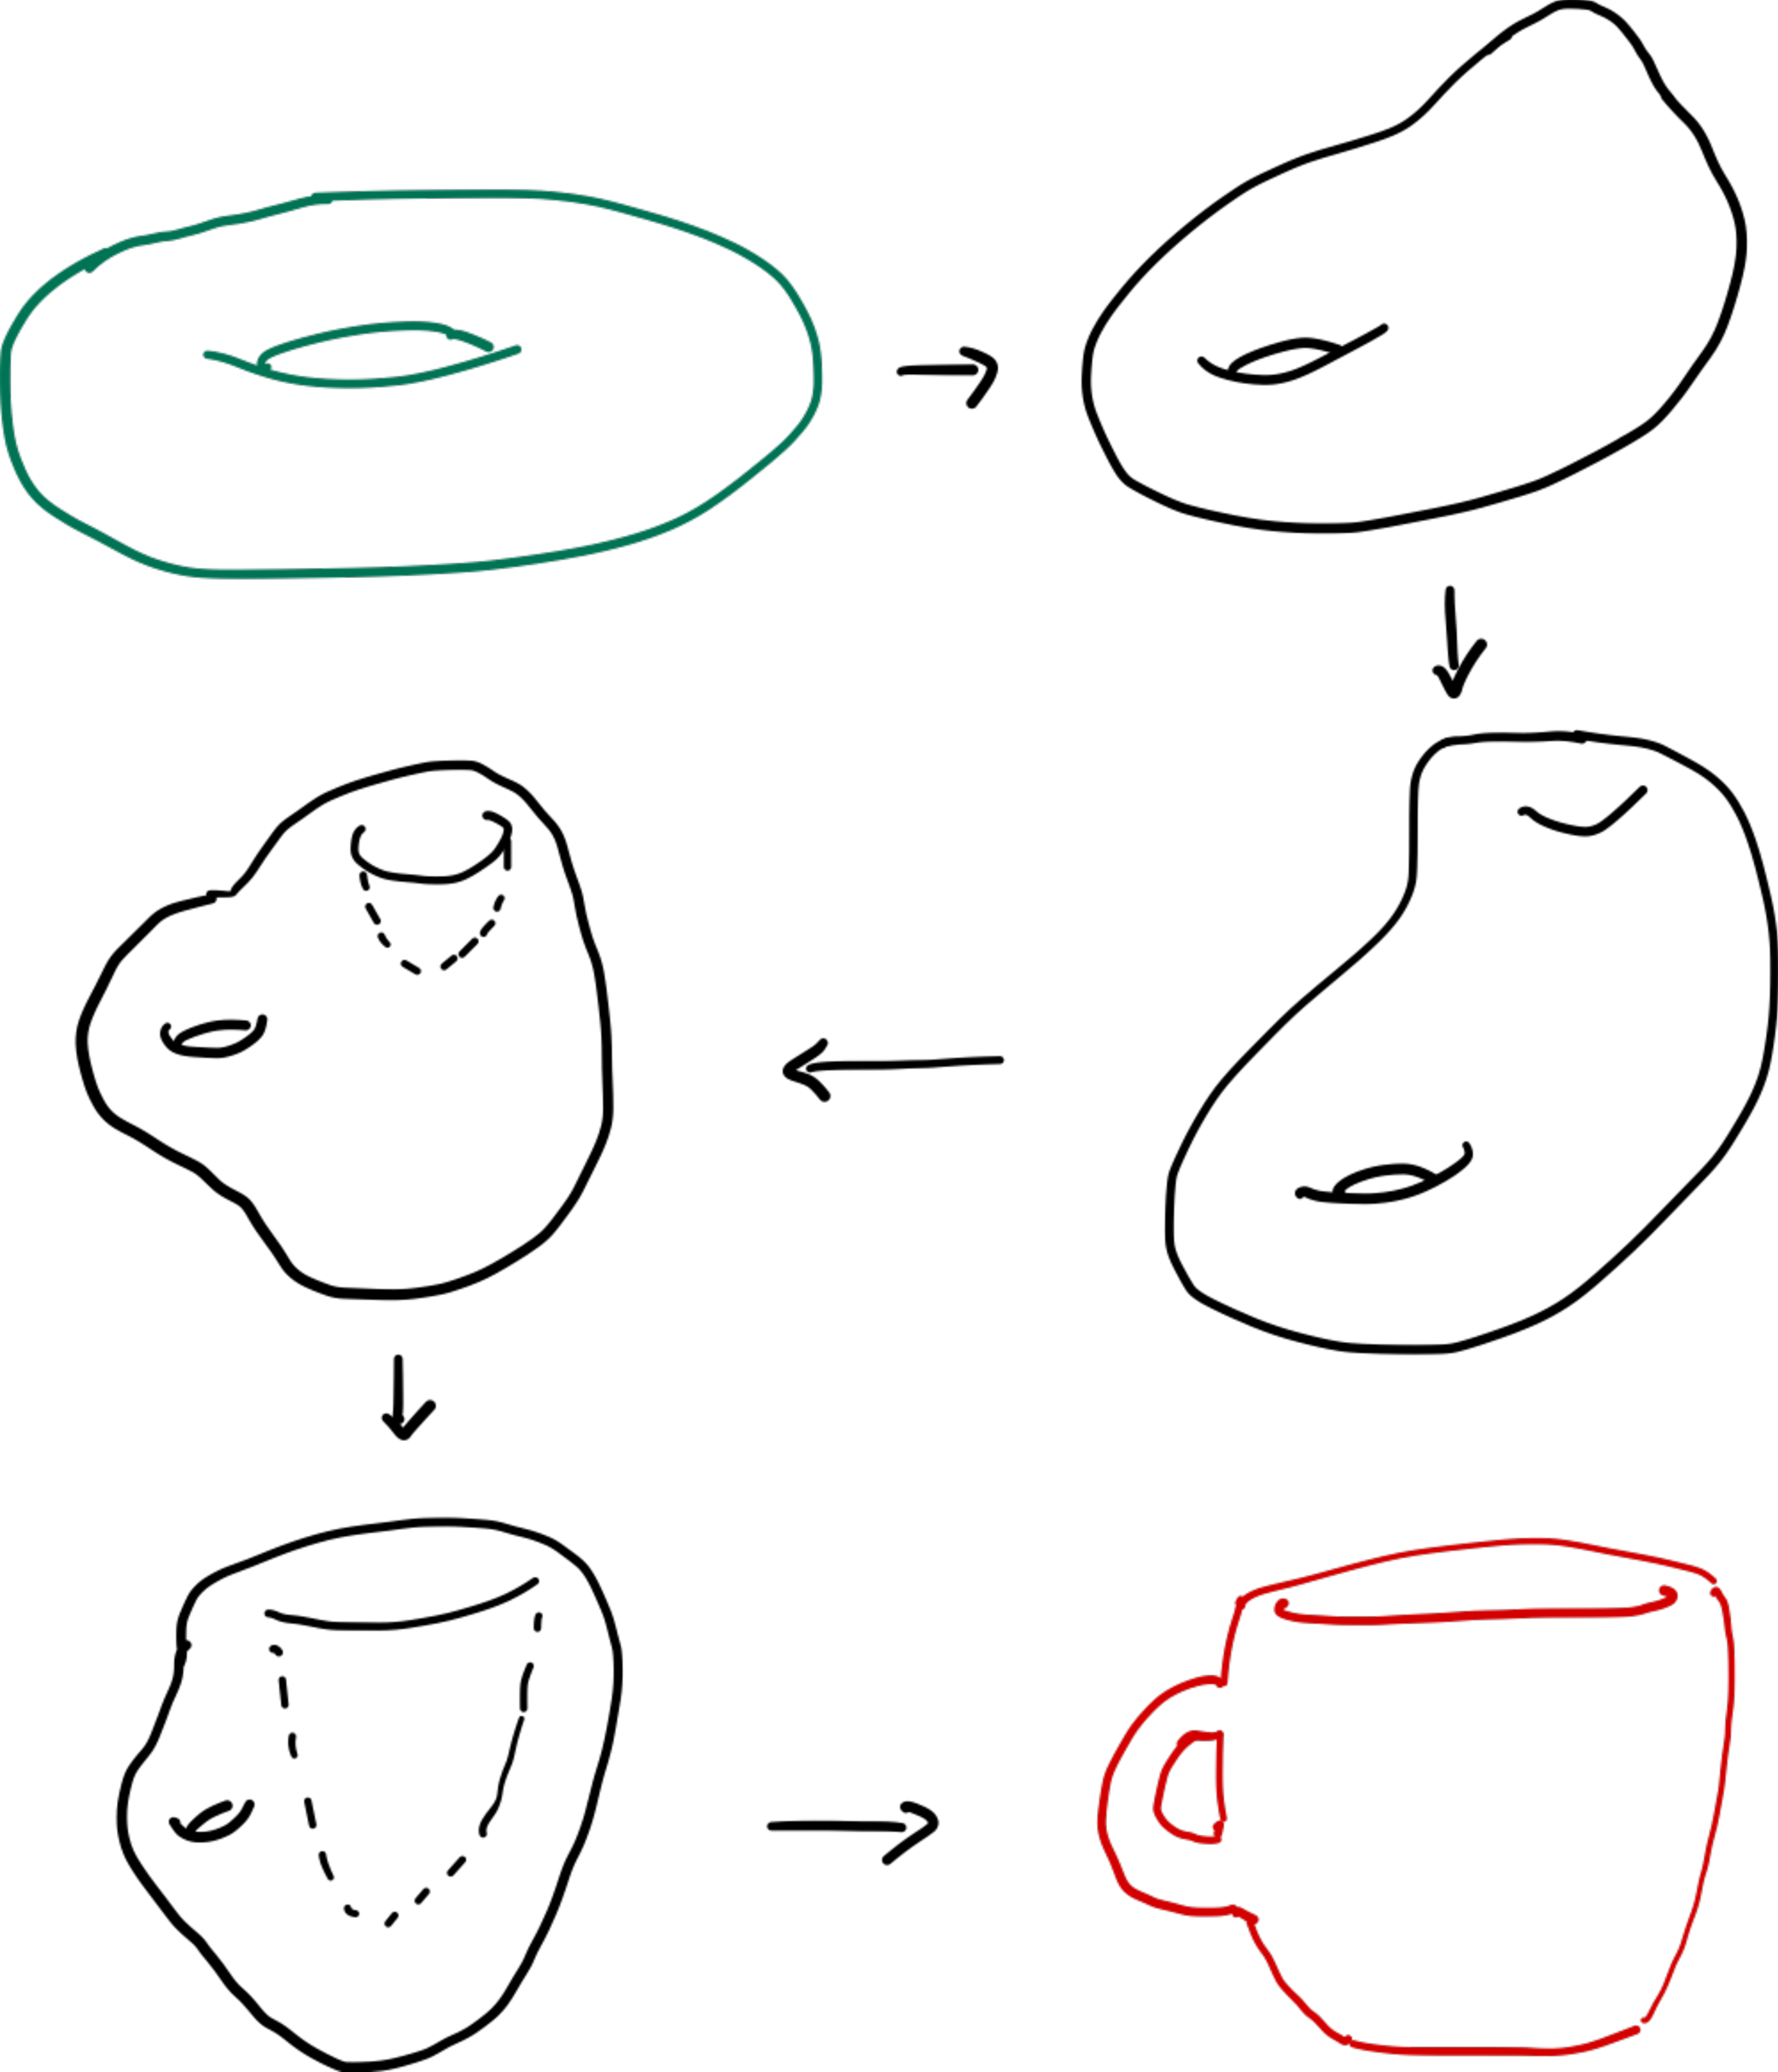
\includegraphics{images/1_1-dount-to-cup.pdf}
  \vspace{5pt}
\end{marginfigure}

\begin{definition}
  A topological space $(X, \cT)$ is \emph{Hausdorff} if every two distinct points admit disjoint open neighbourhoods. That is, for every pair $x\neq y$ of points in $X$, there exist open subsets $U_x, U_y\in\cT$ such that $x\in U_x$, $y\in U_y$ and $U_x \cap U_y = \emptyset$.
\end{definition}

Topological spaces are extremely general, as such they may have very inconvenient---someone may say nasty---properties.
You can see this for yourself with the following exercise.

\begin{exercise}
  \begin{itemize}
    \item Let $X$ be an arbitrary set. Show that $\cT:=\{\emptyset, X\}$ defines a topology on $X$, called the \emph{trivial topology}. Show that on $(X, \cT)$ any sequence in $X$ converges to every point of $X$, and every map from a topological space into $X$ is continuous.
    \item Let $X$ be an arbitrary set. Show that $\cT:=\mathcal{P}(X) := \{ A \mid A\subset X \}$, the powerset of $X$, defines a topology on $X$, called the \emph{discrete topology} in which every map $f : X \to Y$ to some other arbitrary topological space $(Y, \cU)$ is continuous.
  \end{itemize}
\end{exercise}

Hausdorff spaces are still rather general: in particular, any metric space with the metric topology\footnote{Recall that in a metric space $X$ the \emph{metric topology} is defined in the following way: a set $U\subset X$ is called open if for any $x\in U$ there exists $\epsilon>0$ such that $U$ fully contains the ball of radius $\epsilon$ around $x$.} is Hausdorff.

\begin{definition}
  A topological space $(X, \cT)$ is \emph{second countable} if there exists a countable set $\cB\subset\cT$ such that any open set can be written as a union of sets in $\cB$.
  In such case, $\cB$ is called a (countable) basis for the topology $\cT$.
\end{definition}

\begin{exercise}[Euclidean space $\R^n$]\label{exe:rntopsp}
  Let's consider on $\R^n$ the metric topology\footnote{See comment above.} induced by the euclidean metric $d: \R^n \times \R^n \to [0, +\infty)$, $d(x,y) := \sqrt{\sum_{i=1}^n (x^i-y^i)^2}$.
  Show that the topological space defined on $\R^n$ is Hausdorff and second countable.
\end{exercise}

\begin{definition}[Topological manifold]
  A topological space\footnote{From now on, if we say that $X$ is a topological space we are implying that there is a topology $\cT$ defined on $X$.} $M$ is a \emph{topological manifold} of dimension $n$, or topological $n$-manifold, if it has the following properties:
  \marginnote[0.5em]{Note that the finite dimensionality is a somewhat artificial restriction: manifolds can be infinitely dimensional~\cite{book:lang:infinite}. For example, the space of continuous functions between manifolds is a so-called infinite-dimensional Banach manifold.\vspace{1em}}
  \begin{enumerate}[(i)]
    \item $M$ is a Hausdorff space;
    \item $M$ is second countable;
    \item $M$ is \emph{locally euclidean} of dimension $n$, that is\footnote{In words, any point $p\in M$ has a neighbourhood that is homeomorphic to an open subset of $\R^n$.}, for any point $p\in M$ there exist an open subset $U\subset M$ with $p\in U$, and open subset $V\subset\R^n$ and a homeomorphism $\varphi: U\to V$.
  \end{enumerate}
\end{definition}

\begin{notation}
  Reusing the notation of the definition above, we call \emph{(coordinate) chart} the pair $(U, \varphi)$ of a \emph{coordinate neighbourhood} $U$ and an associated \emph{coordinate map}\footnote{Or \emph{coordinate system}.} $\varphi: U\to V$ onto an open subset $V=\varphi(U)\subseteq\R^n$ of $\R^n$.
  Furthermore, we say that a chart is \emph{centred at $p\in U$} if $\varphi(p) = 0$.
\end{notation}

\begin{figure}[htp]
  \centering
  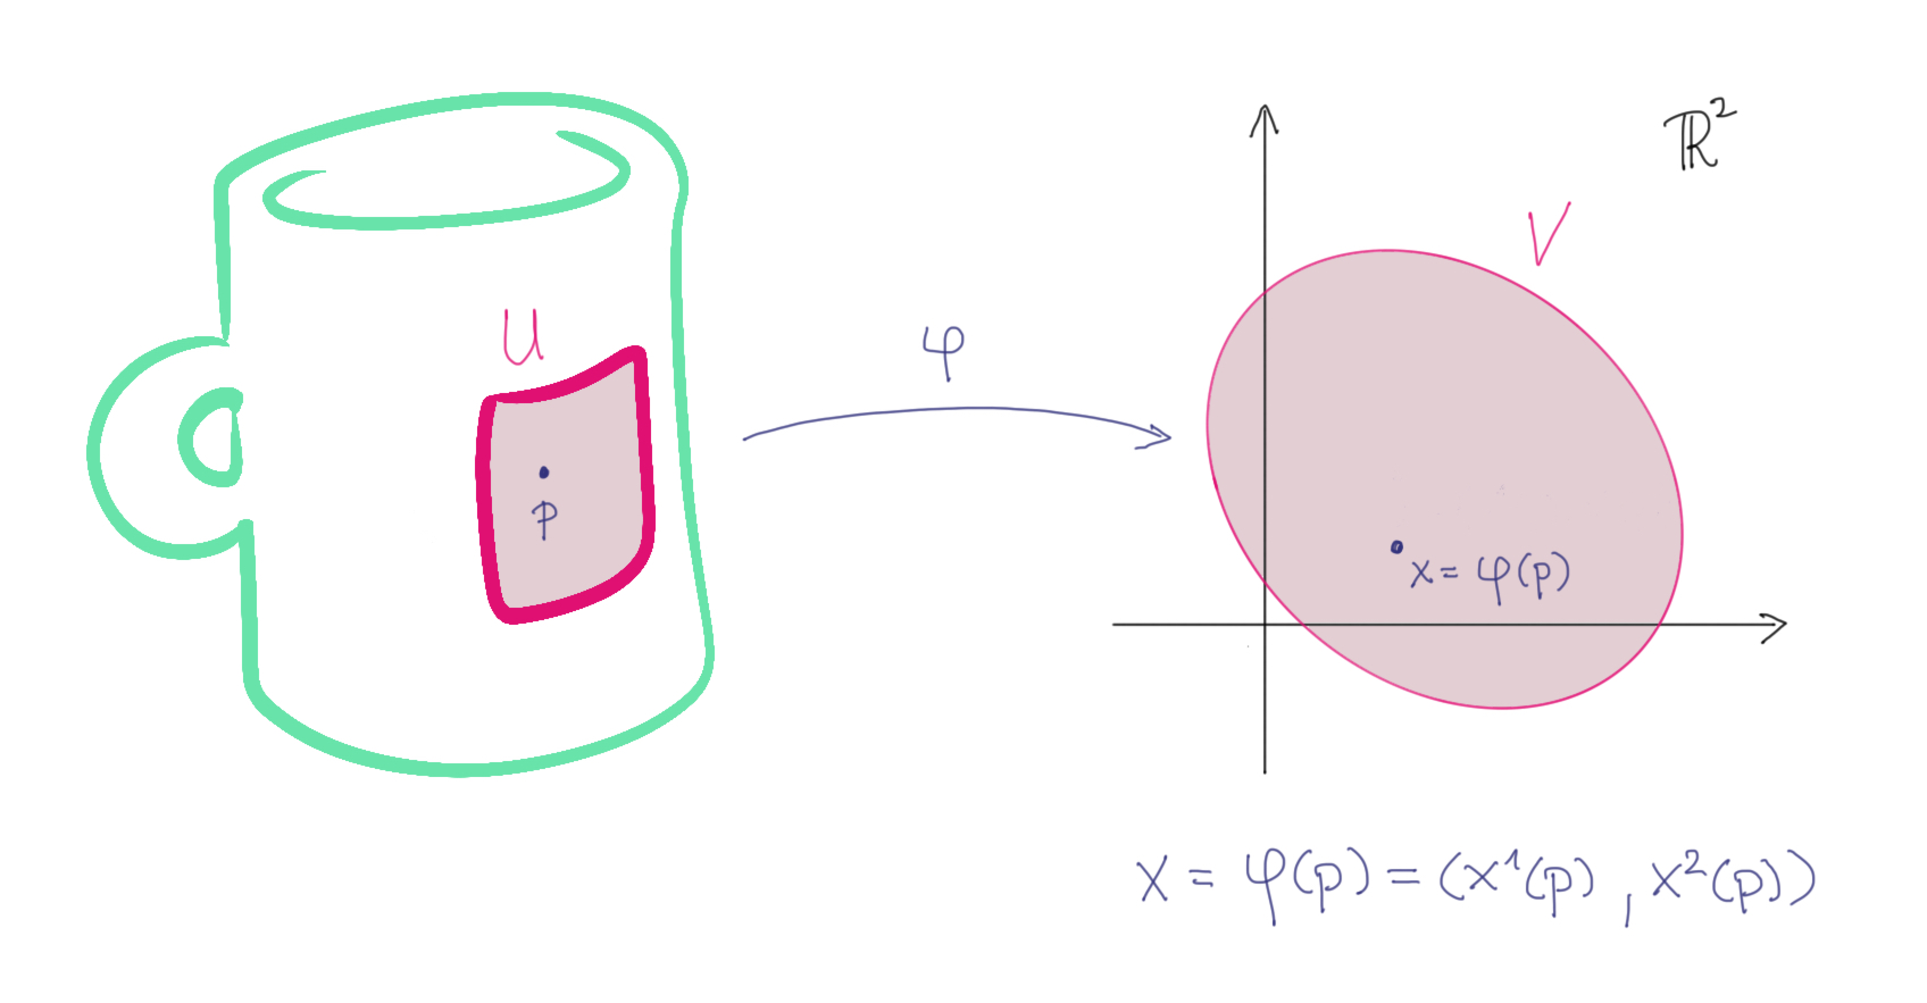
\includegraphics{1_2-charts.pdf}
  \caption{Being locally euclidean allows to define coordinates on the manifold, that is, a mapping between the manifold and the euclidean space.}
  \label{fig:1.2-charts}
\end{figure}

Don't get scared by conditions (i) and (ii) in the definition of topological manifolds: they are only needed to make sure that there are not too few open sets (Hausdorff) and not too many (second countable).

\begin{example}
  With our definition, a countable collections of points with the discrete topology is a $0$-dimensional topological manifold.
  An uncountable collection of points with the discrete topology, however, is not!
\end{example}

\begin{example}
  $\R^n$ is trivially\footnote{Use Exercise~\ref{exe:rntopsp} and the \emph{global} chart $(\R^n, \id_{\R^n})$, where $\id_{\R^n}(x) := x$ is the identity on $\R^n$.} a topological manifold of dimension $n$.
  More generally, any $n$-dimensional vector space\footnote{In fact, any open subset of a $n$-dimensional vector space.} is a topological $n$-manifold.
\end{example}

\begin{exercise}[The line with two origins]
  Even though $\R^n$ with the euclidean topology is Hausdorff, being Hausdorff does not follow from being locally euclidean. A famous counterexample is the following\footnote{See also \cite[Problem 1-1]{book:lee} and \cite[Problem 5.1]{book:tu}.}.
  \begin{marginfigure}
    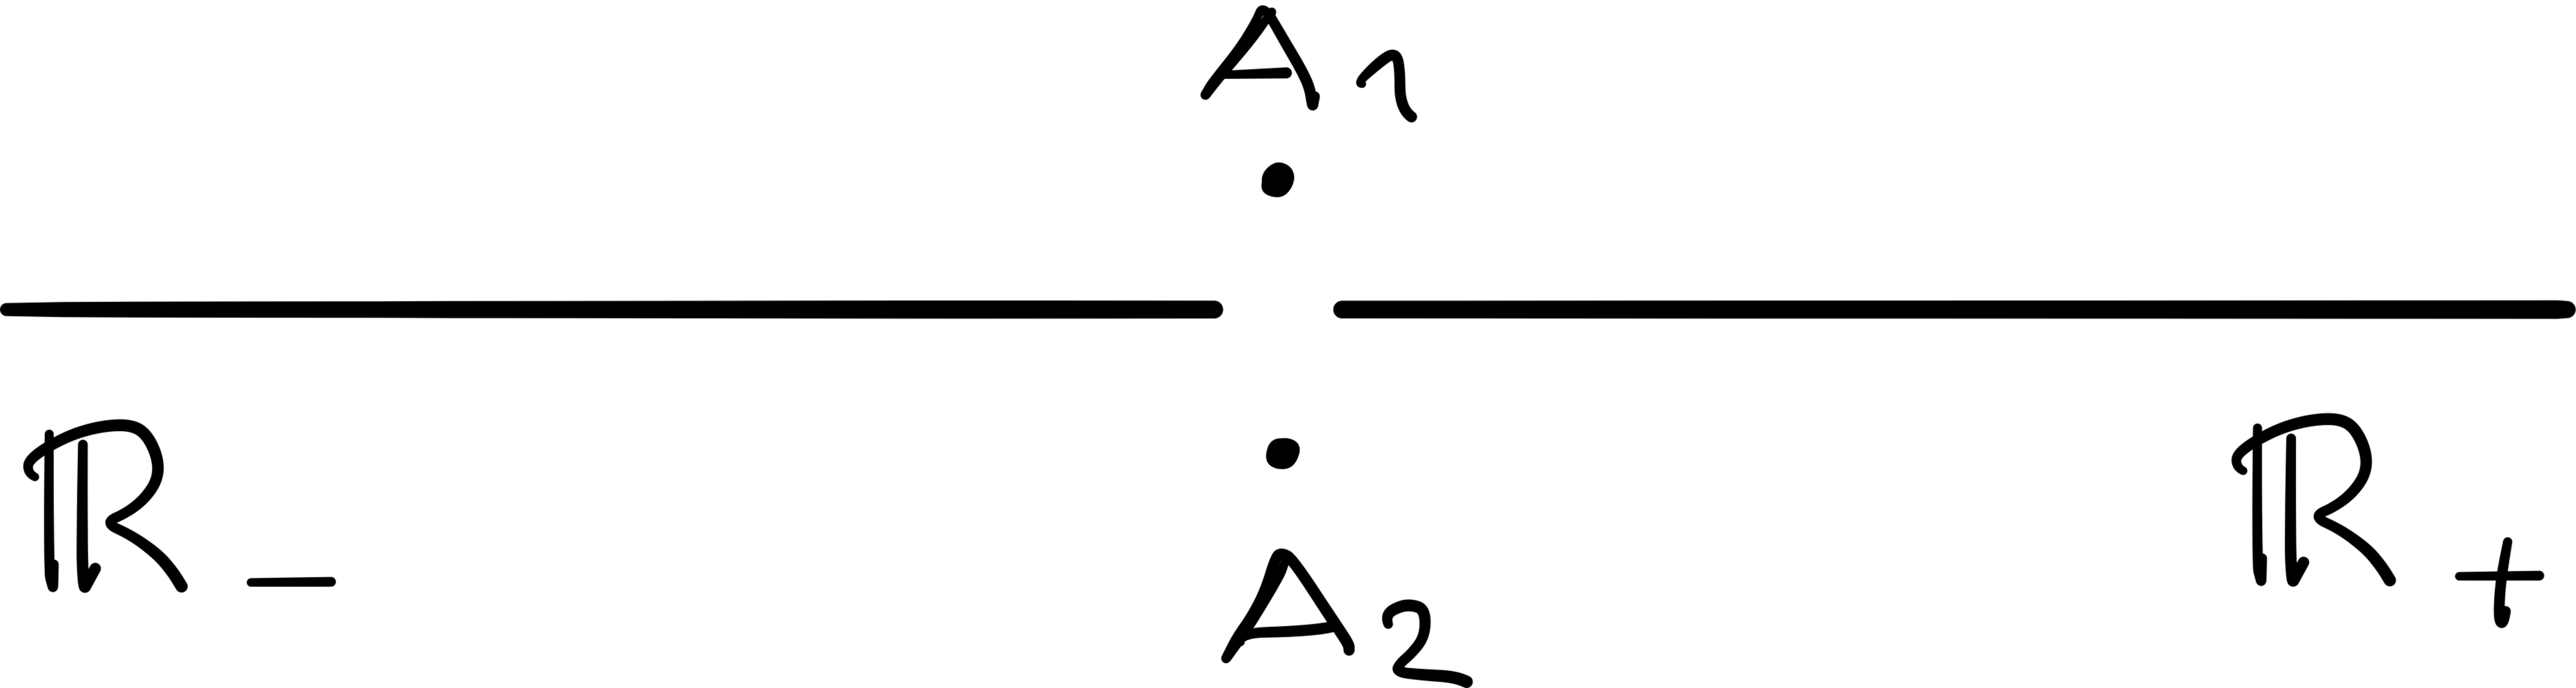
\includegraphics{1_ex_1_0_11.pdf}
    \label{fig:hausdorff-not-locally-euclidean}
    \caption{A locally euclidean space which is not Hausdorff.}
  \end{marginfigure}
  Let $A_1, A_2$ be two points not on the real line $\R$ and define $M:= (\R\setminus\{0\})\cup\{A_1,A_2\}$.
  Induce a topology on $M$ by taking as basis the collection of all open intervals in $\R$ that do not contain $0$, along with all the sets of the form $(-a, 0)\cup\{A_1\}\cup(0,a)$ and $(-a, 0)\cup\{A_2\}\cup(0,a)$, for $a>0$.
  \begin{enumerate}
    \item Check that this forms a basis\footnote{That is, the basis elements cover $M$ and for any $B_1, B_2$ on the basis, for all $x \in I = B_1\cap B_2$, there is an element $B_3$ of the basis such that $x\in B_3$ and $B_3\subset I$.} for a topology on $M$.
    \item Define the two charts
      \begin{equation}
        \varphi_j:(\R\setminus\{0\})\cup\{A_j\} \to \R, \quad
        \varphi_j(x) = \begin{cases} x &\mbox{if } x\neq A_j\\ 0 & \mbox{if } x = A_j \end{cases}, \quad
        j = 1,2.
      \end{equation}
      Show that $\varphi_1$ and $\varphi_2$ are homeomorphisms with respect to the aforementioned topology. 
      %induced by the two charts\footnote{Let $(X, \cT)$ be a topological space and $f: X\to Y$ some map. The induced topology on $Y$ is \begin{equation}\cU_f := \{f^{-1}(U) \;\mid\; U\in\cT\}.\end{equation}}.
    \item Show that $M$ is locally euclidean and second countable but not Hausdorff.
  \end{enumerate}
\end{exercise}

\begin{example}\label{ex:uball}
  The \emph{closed} unit ball $D_1(0)$, where similarly as before
  \begin{equation}
    D_r(x) := \{z\in\R^n \;\mid\; d(z,x) \leq r\},
  \end{equation}
  is \emph{not} a topological manifold of dimension $n$. Can you see why? In fact, this is an example of a more general concept of \emph{manifold with boundary} that we will introduce later in Chapter~\ref{sec:mbnd}.
\end{example}

\begin{example}
  Consider the set $M := \{ x\in\R^2 \;\mid\; |x^1| = |x^2| \}$ with the topology induced by $\R^2$:
  this is \emph{not} a topological manifold.
  Since the number of connected components is invariant under homeomorphisms, open connected neighbourhoods of $(0,0)\in M$ cannot be\footnote{A drawing of $M$ is worth more than a hundred words.} homeomorphically mapped to open connected sets in $\R$.
\end{example}

\newthought{There is still an elephant in the room} in need of a comment.
In our definition of topological manifolds, we are taking for granted that the dimension of the manifold is well--defined, that is, if we have two different charts, $\varphi_1: U \to \R^n$ and $\varphi_2: U \to \R^m$, then necessarily $m=n$. Luckily this is true! The result is called \emph{Invariance Domain Theorem} and, since its proof requires advanced concepts of algebraic topology, we will not pursue it further in the course.
\marginnote[-2em]{There is a caveat, the theorem holds for \emph{connected} components of a manifold. If you consider two distinct connected components, you can indeed have different dimensions for each of them.}

\section{Differentiable manifolds}

Before entering into the details of new definitions, let's recall what will be the most important tools throughout the rest of the course.

\begin{definition}
  A map $f: U \to V$ between open sets $U\subset\R^n$ and $V\subset\R^m$ is in $C^r(U,V)$ or \emph{of class $C^r$}, if it is continuously differentiable $r$-times.
  It is called a $C^r$-\emph{diffeomorphism}\footnote{With this definition a homeomorphism is a $C^0$-diffeomorphism} if it is bijective and of class $C^r$ with inverse of class $C^r$.
  We say that $f$ is \emph{smooth}, or of class $C^\infty$, if it is of class $C^r$ for every $r \geq 1$.
\end{definition}

\begin{theorem}[Chain rule]\label{thm:chainrule}
  Let $U\subset\R^n$ and $V\subset\R^k$ be open sets and $f: U \to \R^k$, $g: V\to\R^m$ two continuously differentiable functions such that $f(U)\subset V$.
  Then, the following holds.
  \begin{enumerate}[(i)]
    \item\label{thm:chainrule1} The function $g\circ f: U\subset\R^n \to\R^m$ is continuously differentiable and its total derivative~\eqref{eq:jacobian} at a point $x\in U$ is given by
      \begin{equation}
        D(g\circ f)(x) = (Dg)(f(x)) \circ Df(x).
      \end{equation}
    \item\label{thm:chainrule2} Denote $x=(x^1, \ldots, x^n)\in\R^n$ and $y=(y^1,\ldots,y^k)\in\R^k$ the coordinates on the respective euclidean spaces and $f=(f^1,\ldots,f^k)$ and $g=(g^1,\ldots,g^m)$ the components of the functions. Then the partial derivatives of $g\circ f$ are given by
      \begin{equation}
        \frac{\partial g^i\circ f}{\partial x^j}(x)
        = \sum_{r=1}^k \frac{\partial g^i}{\partial y^r}(f(x)) \frac{\partial f^r}{\partial x^j}(x),
        \qquad 1\leq i \leq m,\; 1\leq j\leq n.
      \end{equation}
  \end{enumerate}
\end{theorem}
\marginnote[-5em]{Using Einstein's notation, this could be written as \begin{equation}\frac{\partial (g^i\circ f)}{\partial x^j}(x) = \frac{\partial g^i}{\partial y^r}(f(x)) \frac{\partial f^r}{\partial x^j}(x).\end{equation}}

Theorem~\ref{thm:chainrule} has some very deep consequences.
\begin{exercise}
  Under the hypotheses of the previous theorem, prove the following statements.
  \begin{enumerate}
    \item composition preserves the regularity: that is, the composition of functions of class $C^r$ is itself a function of class $C^r$;
    \item if $f:U\subset\R^n\to V\subset\R^m$ is a diffeomorphism, then $n=m$.
  \end{enumerate}
  \textit{\small Hint: is $Df(x)$ an invertible matrix? If so, what is its inverse?} %$D(f^{-1})(f(x))$.
\end{exercise}

Since differentiability is a \emph{local} property and topological manifolds are \emph{locally} like euclidean spaces, it seems reasonable to expect that we can lift the definitions directly from $\R^n$ using the charts to obtain functions between euclidean spaces:
for example, if we are given a continuous map between two topological manifolds, we can locally view it as a continuous map between two euclidean spaces.
Generalizing this further, we could conceivably say that our original map is differentiable if the local map is.

\newthought{As usual, the devil is in the details}: a topological manifold is only homeomorphic to a euclidean space, and a different choice of homeomorphism might affect whether the local map is differentiable or not.
We need to take extra care to ensure that these lifted definitions keep making sense when we use different charts that overlap.

The solution is to introduce a little more structure to the problem.

\begin{definition}\label{def:crcomp}
  We say that two charts $(U_1, \varphi_1)$ and $(U_2, \varphi_2)$ on a topological manifold $M$ are \emph{compatible} if either $U_1 \cap U_2 = \emptyset$ or if the \emph{transition map}\footnote{Both the composition maps $\varphi_1 \circ \varphi_2^{-1}$ and $\varphi_2 \circ \varphi_1^{-1}$ are called transition maps. Both maps are necessarily homeomorphisms since $\varphi_1$ and $\varphi_2$ are.}
  \begin{equation}
    \varphi_1 \circ \varphi_2^{-1} : \varphi_2(U_1\cap U_2) \to \varphi_1(U_1 \cap U_2)
  \end{equation}
  is a smooth diffeomorphism.
\end{definition}

\begin{figure*}[htp]
  \centering
  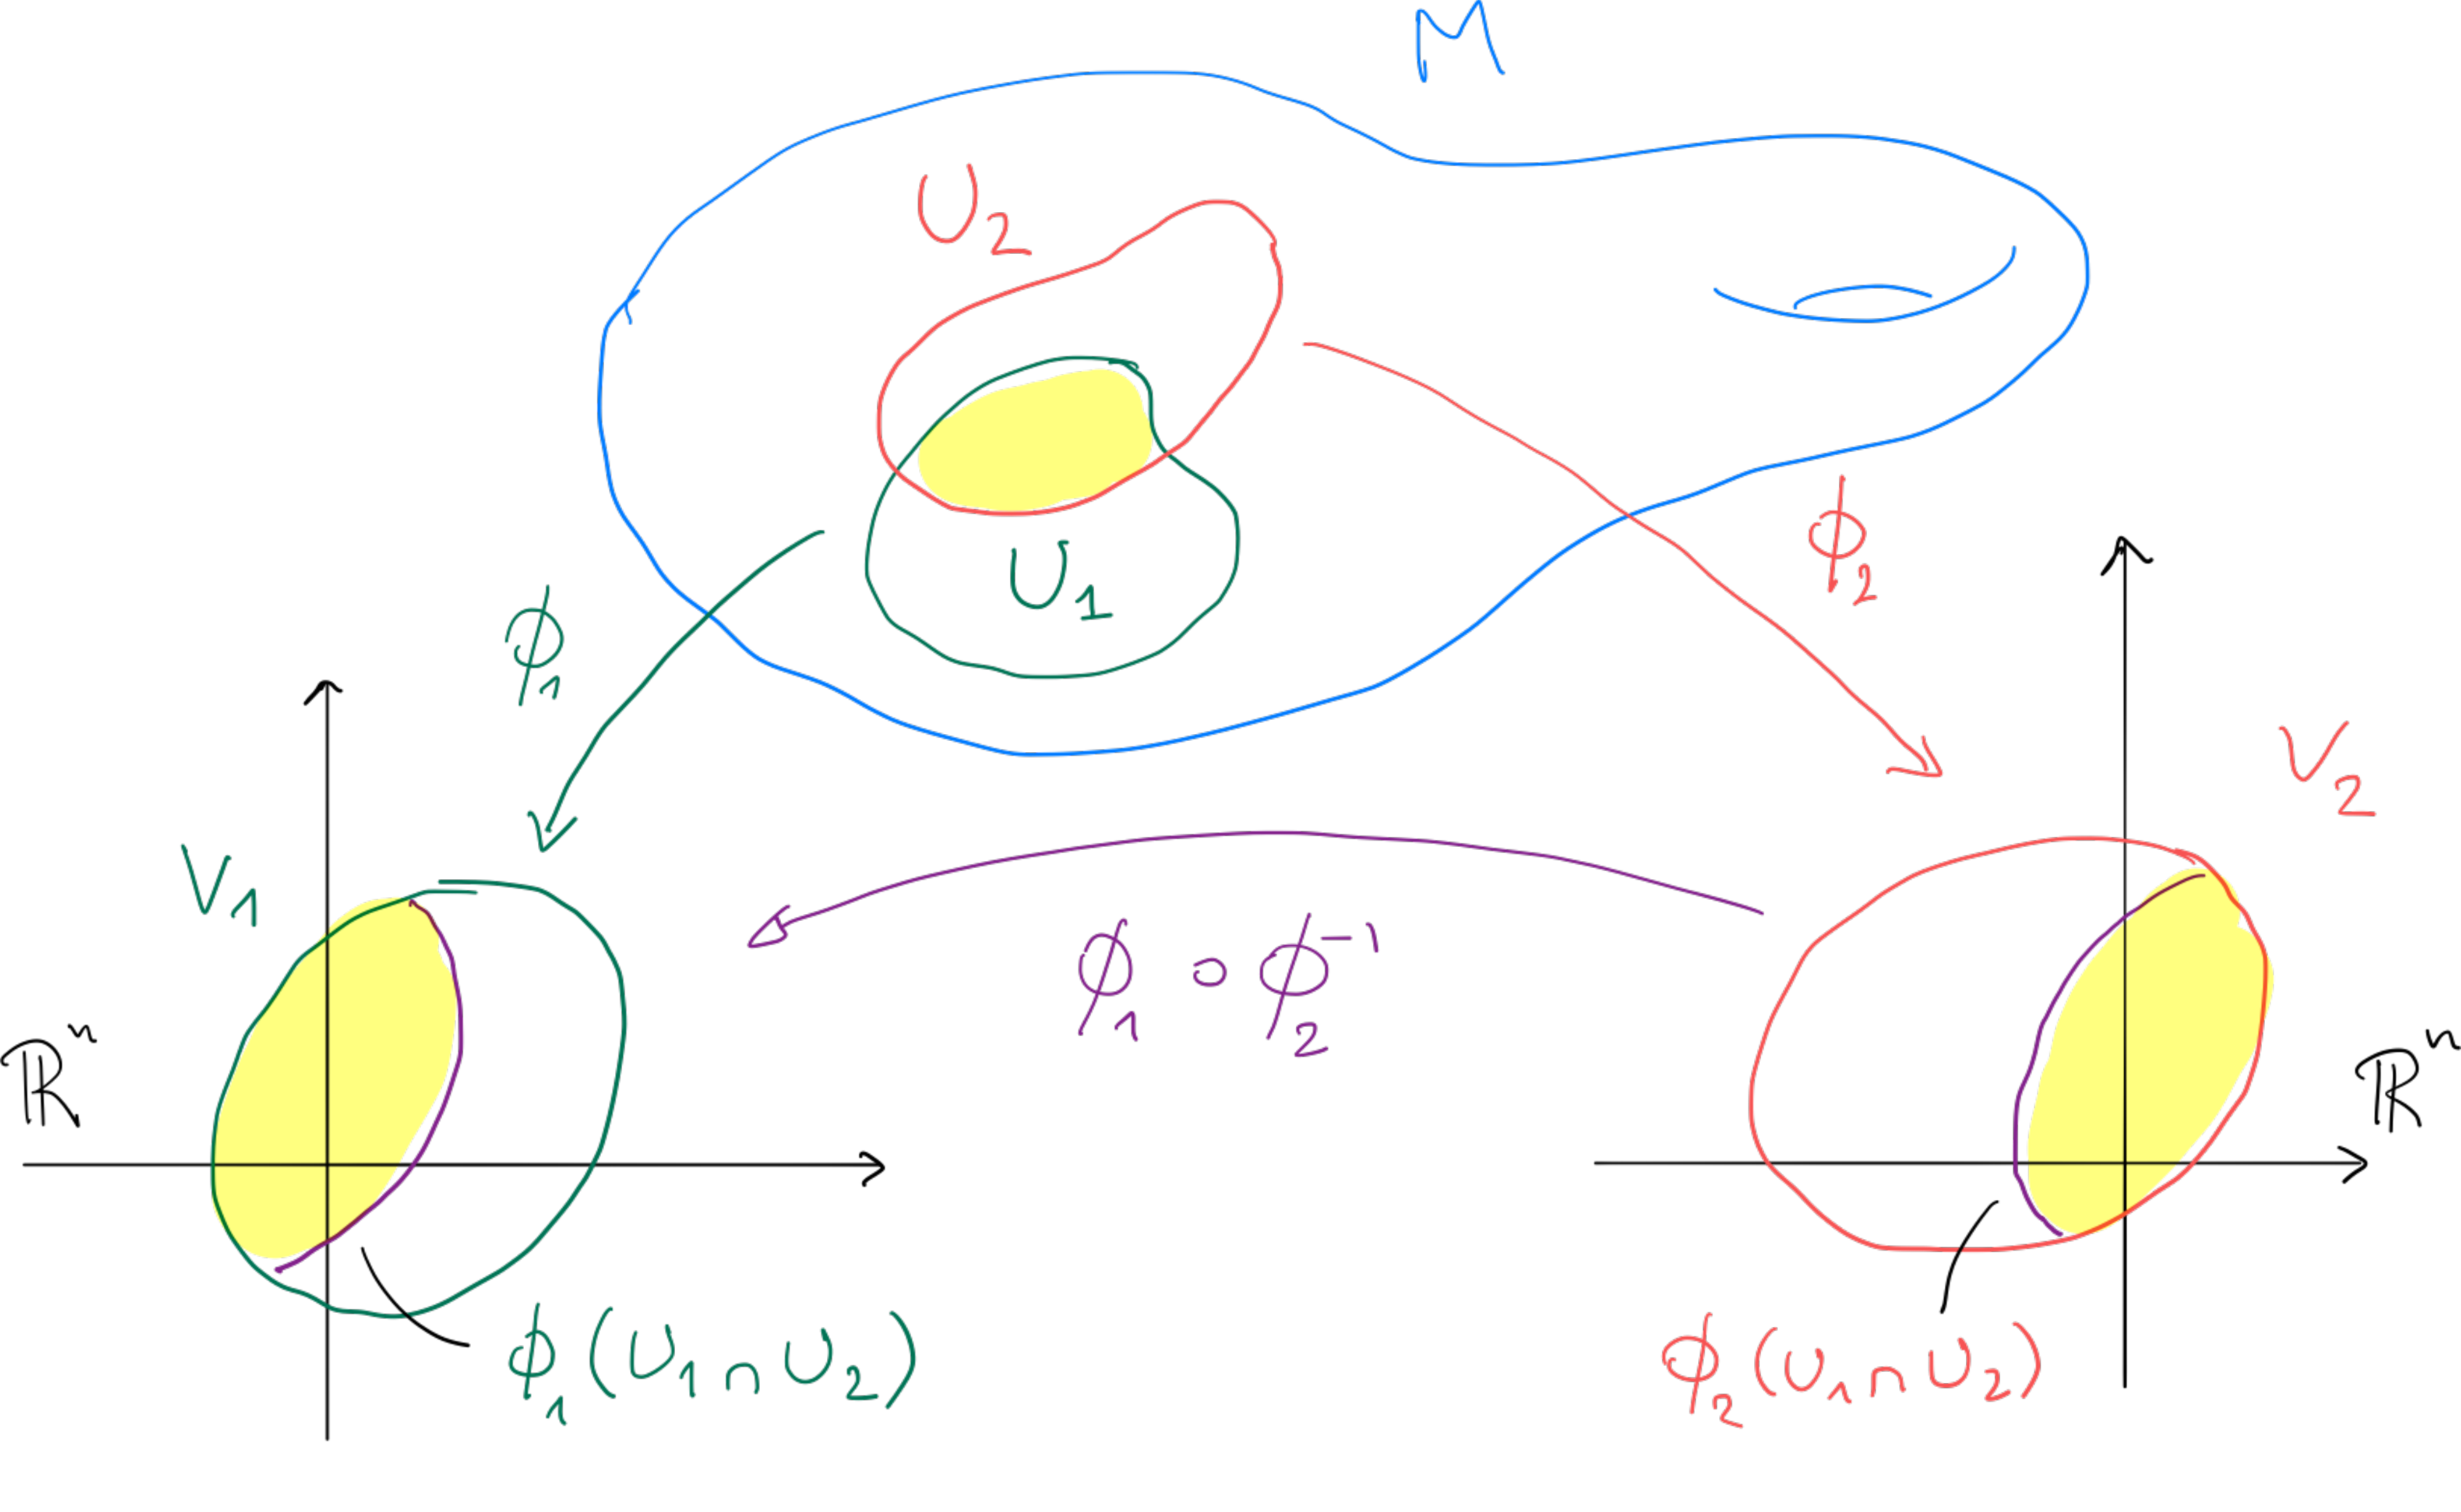
\includegraphics{1_2-compatible-charts.pdf}
  \caption{Charts are compatible if they coincide on the intersections of their coordinate neighbourhoods.}
  \label{fig:1.2-compatible-charts}
\end{figure*}

With these at hand, let's jump into the definition of smooth manifolds.

\begin{definition}\label{def:cratlas}
  A \emph{smooth atlas} is a collection
  \begin{equation}
    \cA = \{\varphi_\alpha: U_\alpha \to V_\alpha \;\mid\; \alpha\in A\}
  \end{equation}
  of pairwise compatible charts that cover\footnote{I.e. such that $M = \cup_{\alpha\in A} U_\alpha$. One calls the set $\{U_\alpha \;\mid\; \alpha\in A\}$, covering $M$ with open sets, an \emph{open cover} of $M$. Here $A$ is some index set, not necessarily countable.} $M$.

  Two smooth atlases are \emph{equivalent} if their union is also a smooth atlas. That is if any two charts in the atlases are compatible.
\end{definition}

\begin{exercise}
  Show that the equivalence of atlases is really an equivalence relation.
\end{exercise}

\begin{definition}\label{def:diffstr}
  \marginnote{The union of all atlases in a differentiable structure is the \emph{unique} \emph{maximal} atlas in the equivalence class.
  There is a one-to-one correspondence between differentiable structures and maximal differentiable atlases \cite[Proposition 1.17]{book:lee}: for convenience and to lighten the notation, from now on, we will always regard a differentiable structure as a differentiable maximal atlas without further comments.}
  A \emph{differentiable structure}, or more precisely a \emph{smooth structure}, on a topological manifold is an equivalence class of smooth atlases.
\end{definition}

\begin{notation}
  By a \emph{chart $(U, \varphi)$ about $p$} in a manifold $M$ we mean a chart in the differentiable structure of $M$ such that $p\in U$.
\end{notation}

\begin{definition}\label{def:diffmanifold}
  A \emph{smooth manifold} of dimension $n$ is a pair $(M, \cA)$ of a topological $n$-manifold $M$ and a smooth structure $\cA$ on $M$.
  \marginnote[1em]{There are no preferred coordinate charts on a manifold: all coordinate systems compatible with the differentiable structure are on equal footing.}
\end{definition}

In colloquial language, a differentiable manifold is just a space covered by charts with differentiable transition maps.
Note that not all topological manifolds can be made into smooth manifolds, but counterexamples are hard to construct and you need at least to go to dimension 4.
A nice and super compact explanation with the relevant reference is in \cite{SE2691140}.

\begin{notation}
  Whenever possible we will omit the differentiable structure $\cA$ from the notation and just write $M$.
  We may write $M^n$ when we want to emphasize that the dimension of $M$ is $n$.
\end{notation}

\begin{exercise}
  Show that on a second countable differentiable manifold it is always possible to find a countable atlas.
\end{exercise}

\begin{exercise}\label{exe:subsetsmanifolds}
  $\R^n$ with the \emph{standard} smooth structure $\cA=\{(\R^n, \id_{\R^n})\}$ is trivially a smooth manifold of dimension $n$.
  %
  In fact, any open subset $U\subset\R^n$ can be made into a smooth manifold in a natural way with the atlas $\cA=(U, \id_{\R^n}|_U)$.

  In the same way, show that any open subset $U$ of a smooth manifold $M$ is a smooth manifold.
  Which atlas would you choose?

  More generally, if $V$ is any $n$-dimensional real vector space, then the standard smooth structure on $V$ is the one induced by the smooth atlas consisting of a single chart $(V, T)$ where $T: V \to \R^n$ is some linear isomorphism.
  Why is this independent of the choice of the isomorphism $T$?

  This fact has a very interesting consequence.
  The space $\mathrm{Mat}(n, \R)$ of real $n\times n$-matrices can be identified with $\R^{n^2}$ by writing the elements of the matrix as a $n^2$-vector.
  This gives to $\mathrm{Mat}(n, \R)$ a structure of differentiable manifold.
  The subset of invertible matrices $GL(n) := GL(n, \R) = \{ A \in \mathrm{Mat}(n, \R) \;\mid\; \det A \neq 0\}$, widely known as the \emph{general linear group}, being an open subset of $\mathrm{Mat}(n, \R)$ (why?) is itself a differentiable manifold.
  Is such manifold connected? Why?
\end{exercise}

\vspace{1em}
\begin{notation}\label{ntn:coords}
  We will stick to the notation of~\cite{book:tu}.
  In the context of manifolds, denote $r^i: \R^n\to\R$, $1\leq i\leq n$, the standard coordinates on $\R^n$.
  With this notation, if $e_i$ denotes the $i$th standard basis vector\footnote{Identified with the \emph{point} $(0,\ldots,0,\LaTeXunderbrace{1}_{i\mbox{th component}},0,\ldots,0) \in\R^n$.} in $\R^n$, then $r^i(e_j) = \delta^i_j$.
  \marginnote{The Kronecker delta $\delta_j^i$ is defined by $\delta_j^i = 1$ if $i=j$ and $\delta_j^i = 0$ otherwise.}

  If $(U, \varphi:U\to\R^n)$ is a chart of a manifold, then $x^i = r^i\circ\varphi$ will denote the $i$-th component of $\varphi$ and denote $\varphi = (x^1, \ldots, x^n)$ and, when convenient, $(U,\varphi) = (U, x^1, \ldots, x^n)$ (see also Figure~\ref{fig:1.2-charts}).

  Thus, for $p\in U$, $(x^1(p), \ldots, x^n(p))$ is a point\footnote{By abuse of notation we sometimes omit the $p$. 
  Thus $(x^1, \ldots, x^n)$ can stand either for local coordinates or a point in $\R^n$: which one it is should be clear from the context.} in $\R^n$.
  The functions $x^1, \ldots, x^n$  are called \emph{(local) coordinates} on $U$.
\end{notation}
\vspace{1em}

An advantage of this new notation is that we can talk about coordinates without the need to explicitly reference charts. In other words, we can say
\begin{quote}
  Let $p\in M$ and choose local coordinates $(x^1, \ldots, x^n)$ about $p$...
\end{quote}
or even
\begin{quote}
  Let $x=(x^1, \ldots, x^n)\in M$ be a point in $M$...
\end{quote}
dropping the distinction between $p$ and $x$, both in place of
\begin{quote}
  Let $p \in M$ and $(U, \varphi)$ a chart defined on a neighbourhood $U$ of $p$.
  Let $x^i = r^i \circ\varphi$ denote the components of $\varphi$ with respect to the standard euclidean coordinates\ldots
\end{quote}

\begin{example}\label{ex:S1emb}
  The unit circle
  \begin{equation}
    \bS^1 := \{x\in\R^2 \;\mid\; \|x\|=1\}\subset\R^2
  \end{equation}
  with the relative topology\footnote{Let $(X,\cT)$ be a topological space and $Y\subset X$. The \emph{relative topology} on $Y$ is \begin{equation}\mathcal{V}:=\{V\subset Y\;\mid\;\exists U\in\cT \mbox{ s.t. } V = U \cap Y\}.\end{equation}} is a $1$-dimensional topological manifold.
  To provide the local homeomorphisms to $\R$ and define a smooth structure for $\bS^1$ it is enough to define the following four charts:
  \begin{equation}
    \begin{aligned}
      &V_1 := \{ x^1 > 0 \},\quad \varphi_1: V_1 \to (-1, 1), \quad \varphi_1(x) := x^2,\\
      &V_2 := \{ x^1 < 0 \},\quad \varphi_2: V_2 \to (-1, 1), \quad \varphi_2(x) := x^2,\\
      &V_3 := \{ x^2 > 0 \},\quad \varphi_3: V_3 \to (-1, 1), \quad \varphi_3(x) := x^1,\\
      &V_4 := \{ x^2 < 0 \},\quad \varphi_4: V_4 \to (-1, 1), \quad \varphi_4(x) := x^1.
    \end{aligned}
  \end{equation}
  What do these charts look like?
\end{example}
\begin{exercise}
  In the previous example, show that the corresponding transition functions are smooth.
\end{exercise}

\begin{exercise}
  Let $\{(U_\alpha, \varphi_\alpha)\}$ be the maximal atlas on a manifold $M$.
  For any open set $U\subseteq M$ and any point $p\in U$, prove the existence of a coordinate open set $U_\alpha$ such that $p\in U_\alpha\subset U$.
\end{exercise}

\begin{exercise}
  Let $f: \R^n \to \R^m$ be a smooth map.
  Show that its graph
  \begin{equation}
    \Gamma_f := \{(x, f(x)) \;\mid\; x\in\R^n\} \subset\R^{n+m}
  \end{equation}
  is a smooth manifold of dimension $n$.
\end{exercise}

\begin{example}
  The definition of smooth manifold does not require $M$ to be embedded into some ambient space as in the examples above.
  In fact, we can define the differentiable manifold $\bS^1$ by equipping the topological quotient space\sidenote[][-11em]{
    There is a standard way to induce a topology on a quotient space.
    Let $M$ be a topological space and $\pi:M\to N$ surjective.
    The \emph{quotient topology} on $N$ is given by defining $U\subset N$ to be open if and only if its preimage $\pi^{-1}(U)\subset M$ is open.
    If $\sim$ is an equivalence relation on $M$, the quotient space $M/\!\sim$ is the set of equivalence classes $[p]:=\{q\in M \mid p\sim q\}$ and the projection $\pi: M\to M/\!\sim$, $\pi(p) = [p]$, is a surjective map. Then $U\in M/\!\sim$ is open if $\cup_{[p]\in U} [p] \subset M$ is open.
    Here $\R/\Z$ denotes the quotient space $\R/\!\sim$ where the equivalence relation is induced by the canonical group action of $\Z$ on $\R$, that is, $x\sim y$ if and only if $x-y\in\Z$.
    This means that $[x] = \{x+k \mid k\in\Z\}$ and each interval $[x_0, x_0+1)$ of length $1$ contains exactly one representative per class.
  Note that we are talking about topological spaces: the quotient, in general, does not preserve the Hausdorff property or second countability.} $\R/\Z$ with the two charts
  \begin{equation}\textstyle
    \varphi_1 : \R/\Z \setminus\{[0]\} \to (0,1)
    \quad\mbox{and}\quad
    \varphi_2 : \R/\Z \setminus\{[\frac12]\} \to (-\frac12,\frac12)
  \end{equation}
  which map $[x]\in\R/\Z$ to its representation in $[0,1)$ or $[-\frac12, \frac12)$ respectively.
  The manifold obtained in this way is diffeomorphic to the one defined in Example~\ref{ex:S1emb}.
\end{example}

\begin{example}[Product manifolds]\label{ex:pm}
  Given two manifolds $(M_1, \cA_1)$ and $(M_2, \cA_2)$, we can define the \emph{product manifold} $M_1 \times M_2$ by equipping $M_1 \times M_2$ with the product topology\footnote{Open sets in the product are products of open sets from the respective topological spaces.} and covering the space with the atlas $\{ (U_1\times U_2, (\varphi_1, \varphi_2)) \;\mid\; (U_1, \varphi_1)\in\cA_1, (U_2, \varphi_2)\in \cA_2\}$.
\end{example}

Note that smooth manifolds do not yet have a metric structure: distances between the points are not defined.
However, they are \emph{metrizable}\footnote{In fact, all the topological manifolds are metrizable. This property is far more general and harder to prove~\cite[Theorem 34.1 and Exercise 1 of Chapter 4.36]{book:munkres:topology} or \cite{nlab:urysohn_metrization_theorem}. Note that not all topological spaces are metrizable, for example a space with more than one point endowed with the discrete topology is not. And even if a topological space is metrizable, the metric will be far from unique: for example, proportional metrics generate the same collection of open sets.}: there exists some metric on the manifold that induces the given topology on it.
This allows to always view manifolds as metric spaces.

Instead of always constructing a topological manifold and then specify a smooth structure, it is often convenient to combine these steps into a single construction.
This is especially useful when the initial set is not equipped with a topology.
In this respect, the following lemma provides a welcome shortcut: in brief it says that given a set with suitable ``charts'' that overlap smoothly, we can use those to define both a topology and a smooth structure on the set.

\begin{lemma}[Smooth manifold lemma]\label{lem:manifold_chart}
  Let $M$ be a set. Assume that we are given a collection $\{U_\alpha\mid \alpha\in A\}$ of subsets of $M$ together with bijections $\varphi_\alpha: U_\alpha\to\varphi(U_\alpha)\subseteq\R^n$, where $\varphi(U_\alpha)$ is an open subset of $\R^n$. Assume in addition that the following hold:
  \begin{enumerate}[(i)]
    \item For each $\alpha, \beta \in A$, the sets $\varphi_\alpha(U_\alpha \cap U_\beta)$ and $\varphi_\beta(U_\alpha \cap U_\beta)$ are open in $\R^n$.
    \item If $U_\alpha \cap U_\beta \neq \emptyset$, the map $\varphi_\beta\circ\varphi_\alpha^{-1}: \varphi_\alpha(U_\alpha \cap U_\beta)\to \varphi_\beta(U_\alpha \cap U_\beta)$ is smooth.
    \item Countably many of the sets $U_\alpha$ cover $M$.
    \item If $p\neq q$ are points in $M$, either there exists $\alpha$ such that $p,q\in U_\alpha$ or there exist $\alpha,\beta$ with $U_\alpha\cap U_\beta=\emptyset$ such that $p\in U_\alpha$ and $q\in U_\beta$.
  \end{enumerate}
  Then $M$ has a unique smooth manifold structure such that each $(U_\alpha,\varphi_\alpha)$ is a smooth chart.
\end{lemma}
\begin{exercise}
  Prove Lemma~\ref{lem:manifold_chart}.\\
  \textit{\small Hint: declare all the $\varphi_\alpha$ to be homeomorphisms and use the hypotheses to check the definition of a smooth manifold.}
\end{exercise}

\begin{example}
  Lemma~\ref{lem:manifold_chart} simplifies life a lot.
  Consider the product manifolds from Example~\ref{ex:pm}.
  Since both $M$ and $N$ are smooth manifolds, the product manifold is a $(m+n)$-dimensional smooth manifold with the atlas introduced in the example.

  The proof of this fact is trivial in the sense that each of the maps in the atlas satisfies all the properties of the lemma by construction, after all they are already part of the differentiable structure of a smooth manifold.
\end{example}

\begin{exercise}
  Prove that the $n$-dimensional torus
  \begin{equation}
    \bT^n := \LaTeXunderbrace{\bS^1\times\cdots\times\bS^1}_{n\mbox{ times}} \subset \R^{2n}
  \end{equation}
  is a smooth manifold of dimension $n$.
\end{exercise}

\subsection{Quotient manifolds}

If $M$ is a topological space and $\sim$ an equivalence relation we have seen that it is sometimes possible to define smooth manifolds.
Since in general the quotient does not behave nicely it is convenient to get a few tricks to check if the manifold structure can be preserved.

In this case it is convenient to have some tools to check continuity of functions.

\begin{proposition}
\marginnote{For a proof refer to \cite[Proposition 7.1]{book:tu} or \cite[Theorem 3.70]{book:lee:topology}.}
  Assume $F:X\to Y$ is a map between topological spaces and $\sim$ is an equivalence relation on $X$.
  Let $F$ be constant on each equivalence class $[p]\in X/\!\sim$, and denote $\widetilde F:X/\!\sim\to Y$, $\widetilde F([p]) := F(p)$ for $p\in X$, the map induced by $F$ on the quotient.

  Then, $\widetilde F$ is continuous if and only if $F$ is continuous.
\end{proposition}

Continuity of the projection $\pi: M \to M/\!\sim$ implies that if $M/\!\sim$ is Hausdorff, then $\pi^{-1}(\pi(s)) = [s]$ is closed in $M$.
If, additionally, $\pi$ is open\footnote{That is, it maps open sets to open sets.} then there is a stronger statement:
\marginnote[4em]{These statements are not hard to prove, but their proofs will be omitted here.
You can refer to~\cite[Chapters 7.1--7.5]{book:tu}.}
\begin{theorem}\label{thm:openproj}
  If $M$ is a topological space and $\sim$ an equivalence relation such that $\pi:M \to M/\!\sim$ is open, then:
  \begin{itemize}
    \item $\pi$ maps a basis for the topology of $M$ into a basis for the topology $M/\!\sim$, thus if $M$ is second countable, then $M/\!\sim$ is second countable;
    \item the quotient space $M/\!\sim$ is Hausdorff if and only if the graph $R$ of $\sim$, i.e., the set
      \begin{equation}
        R := \{(x,y)\in M\times M \mid x\sim y\},
      \end{equation}
      is closed in $M\times M$.
  \end{itemize}
\end{theorem}

In general, however, the class of quotient space is too large to admit a good general theory of smooth manifolds.
Yet, there is a family of manifolds that has undergone lots of research and on which a lot can be said: smooth manifolds with certain smooth Lie group actions.
Treating this will be far too much for the course, but we will provide along the way most of the necessary ingredients for you to be able to explore the topic on your own.
For further reference, you can look at~\cite[Chapter 21]{book:lee}.

Before moving on, below we are going to look at a couple of simpler, notable, examples of quotient manifolds.

\begin{example}
  Let $\RP^n$ denote the $n$-dimensional real projective space, that is, the space of lines in $\R^{n+1}$ passing through the origin.
  This is a notable example of quotient manifold: we are going to show that $\RP^n$ is a smooth manifold of dimension $n$. 

  We can define an equivalence relation on $\R^{n+1}_0:=\R^{n+1}\setminus\{0\}$ by declaring that for any $x,y\in \R^{n+1}_0$
  \begin{equation}
    x\sim y \quad\Longleftrightarrow\quad \exists t\neq 0 \mbox{ such that } y=tx,
  \end{equation}
  that is, two points are equivalent if they lie on the same line passing through the origin.
  Then, the \emph{real projective space} is the quotient space $\RP^n := \R^{n+1}_0/\!\sim$.
  For the sake of the example, let's denote the class of equivalence of a point $x=(x^0,\ldots,x^n)\in\R^{n+1}_0$ by $[x]=[x^0,\ldots,x^n]$ and the projection to the quotient by $\pi:\R^{n+1}_0\to\RP^n$.
  The classes of equivalence $[x]$ are called \emph{homogeneous coordinates} on $\RP^n$.

  \begin{marginfigure}
    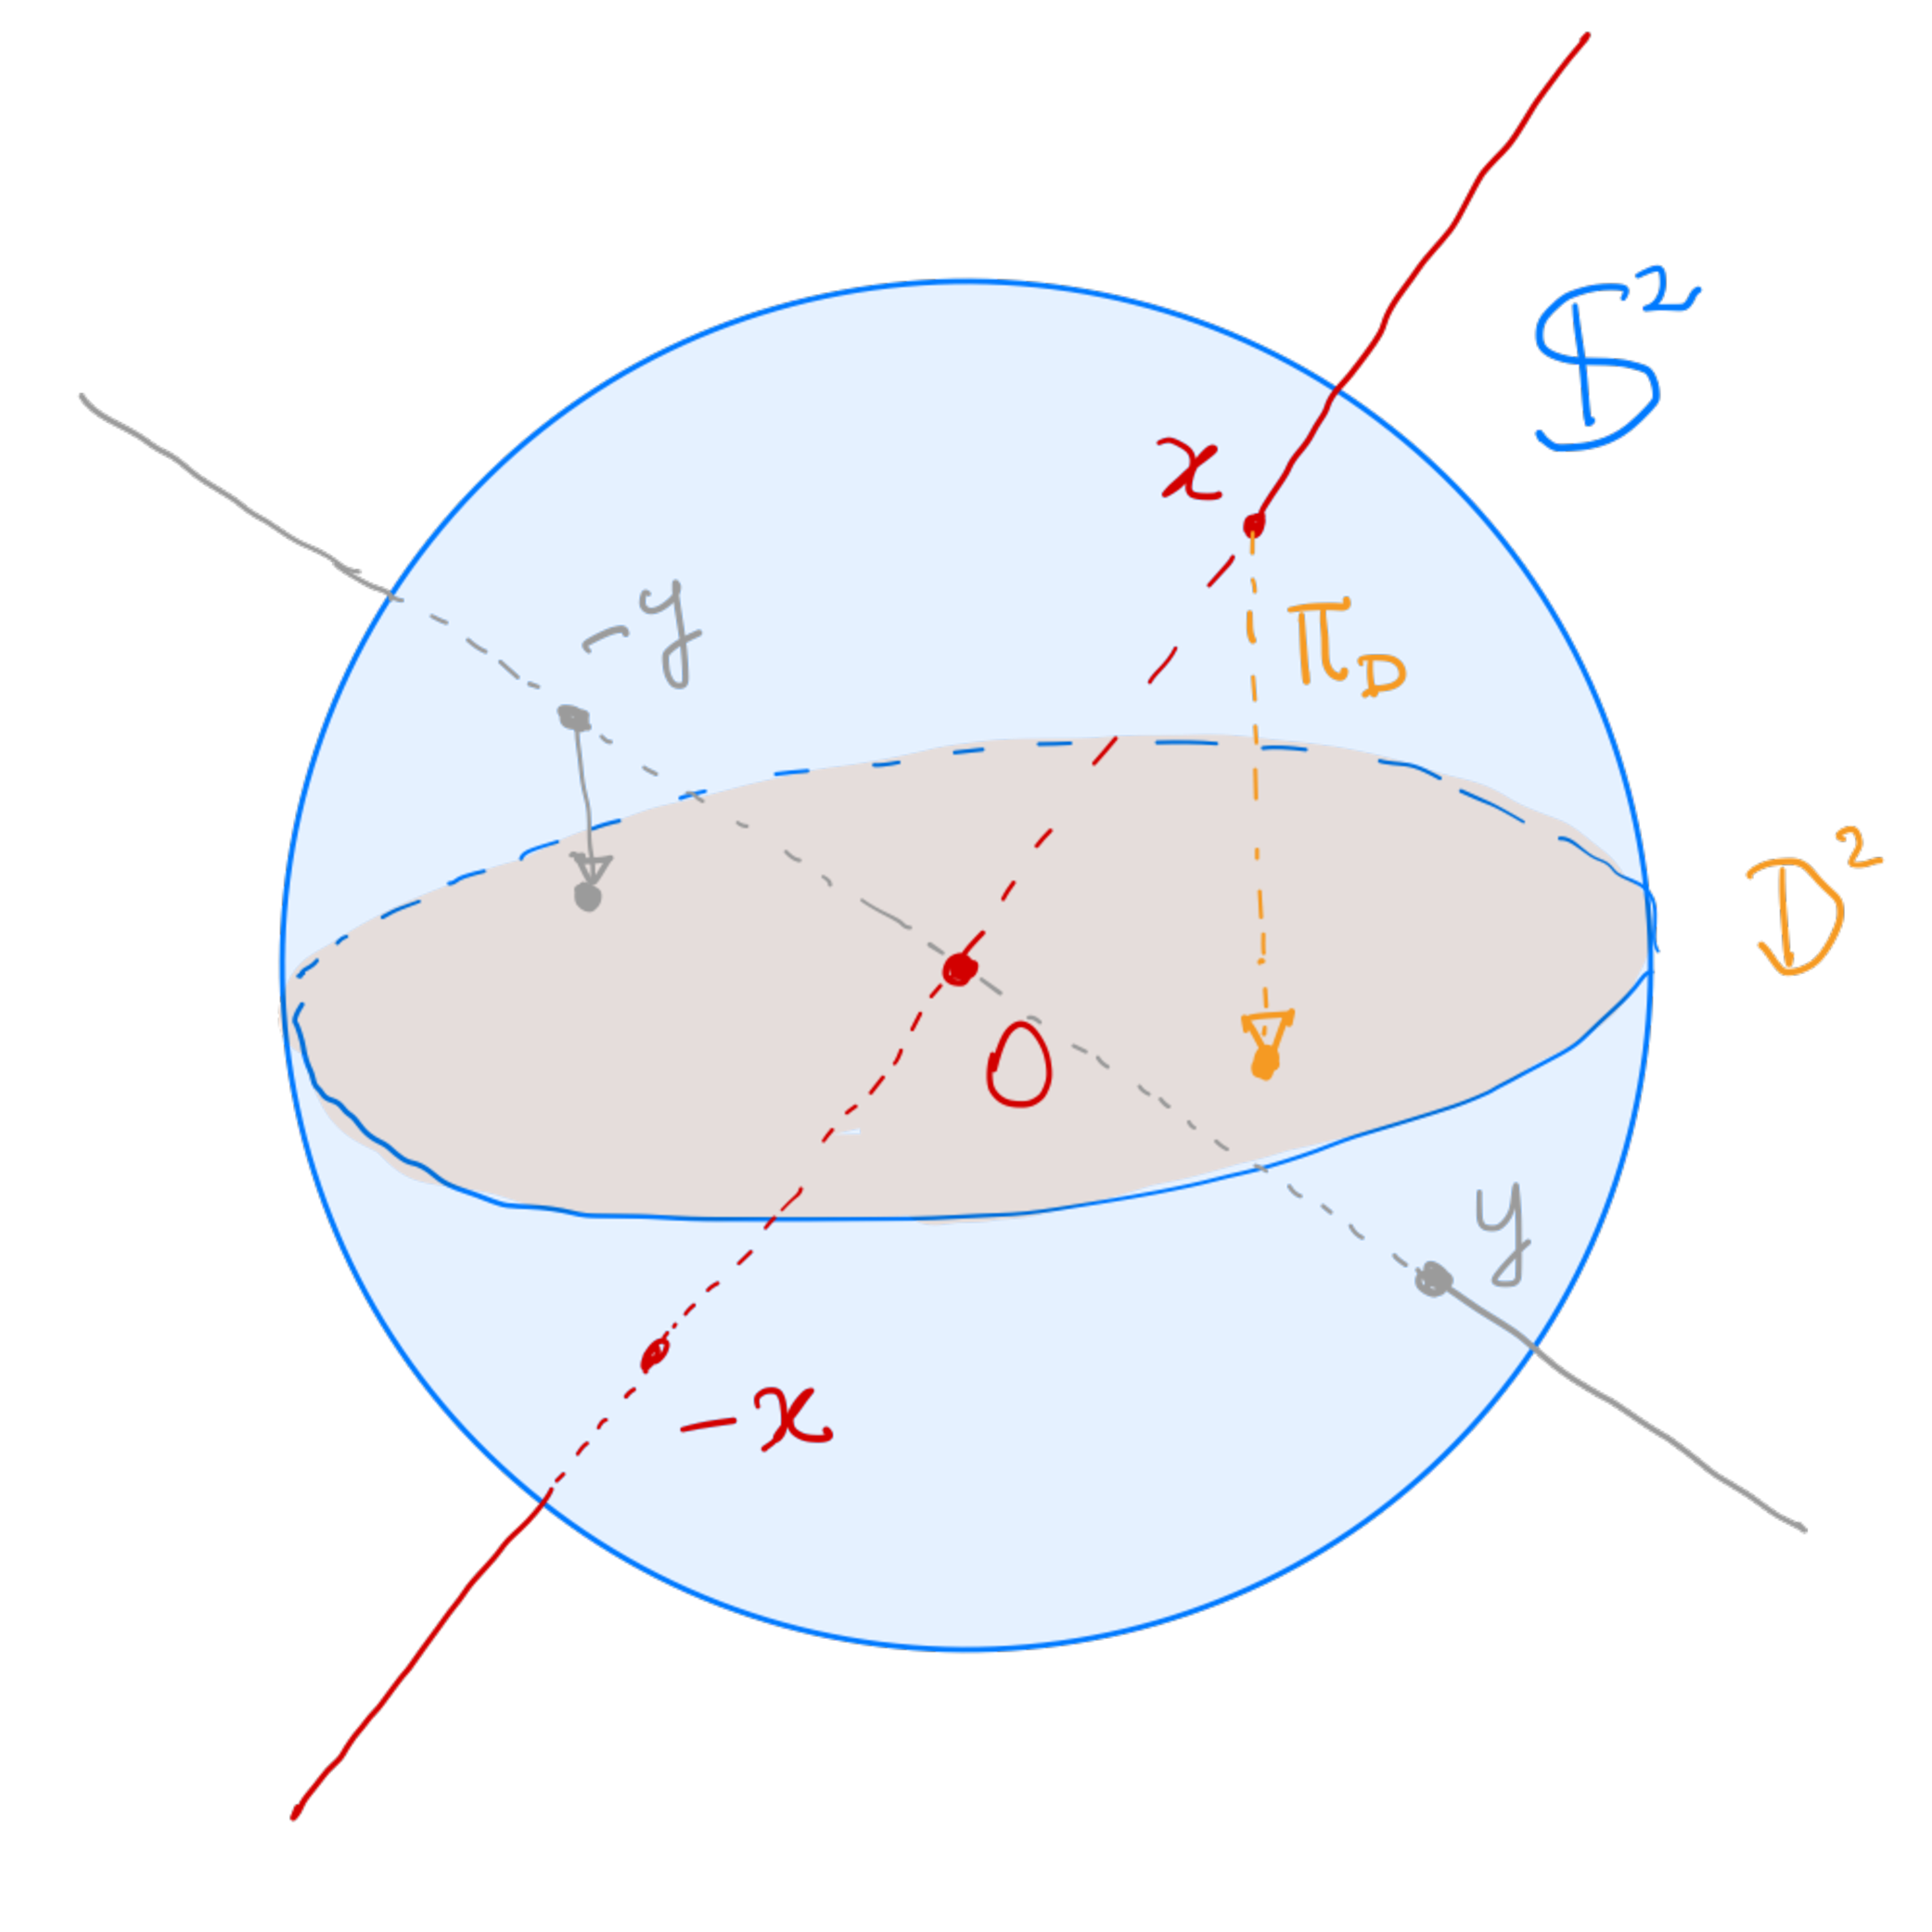
\includegraphics{1_2_25-sphere}
    \caption{The identification $\sim'$ of antipodal points maps the sphere to a disk. Embedding $\bS^n/\!\sim'$ in $\R^{n+1}$, one can define a map $\pi_D$ that projects the representative of $[x]$ in the north hemisphere orthogonally to the disk $D^n = \{x\in\R^{n+1} \mid \|x\|\leq 1, \; x^{n+1}=0\}$ (the equator is mapped to itself). }
  \end{marginfigure}
  There is a nice interpretation of this construction in terms of flattening spheres.
  Observe that a line through the origin always intercepts a sphere $\bS^n$ at two antipodal points and, conversely, each pair of antipodal point determines a unique line through the center.
  So we can define an equivalence relation on the sphere by identifying the antipodal points: given $x,y\in\bS^n$, $x\sim' y$ if and only if $x = \pm y$.
  This leads to the bijection $\RP^n \simeq \bS^n/\!\sim'$.
  Note that by gluing antipodal points, we are identifying the north and south hemispheres, thus essentially flattening the sphere to a disk.

  \begin{exercise}\label{exe:RPSN}
    Show that the map $n: \R^{n+1}_0\to \bS^n$, $n(x) = \frac{x}{\|x\|}$, induces a homeomorphism $\hat n:\RP^n \to \bS^n/\!\sim'$.\\
    \textit{\small Hint: find an inverse map and show that both $\hat n$ and its inverse are continuous.}
  \end{exercise}

  \newthought{Let's first show that $\RP^n$ is a topological $n$-manifold}.
  The structure of topological manifold follows immediately from the Theorem~\ref{thm:openproj} and $\pi$ being open, so let's prove that.

  Let $U\subset\R_0^{n+1}$, since $\pi$ is continuous by construction, $\pi(U)$ is open if $\pi^{-1}(\pi(U))$ is open in $\R^{n+1}_0$.
  By definition
  \begin{equation}
    \pi^{-1}(\pi(U)) = \bigcup_{t\neq 0} tU = \bigcup_{t\neq 0}\{tp \mid p\in U\}.
  \end{equation}
  Since multiplication by $t\neq 0$ is a homeomorphism of $\R_0^{n+1}$, the set $t U$ is open for any $t$, as is their union, $\RP^n$ is both Hausdorff and second-countable.

  For each $i=0,\ldots,n$, define $\widetilde U_i := \{x\in\R^{n+1}_0 \mid x^i\neq0\}$, the set where the $i$-th coordinate is not $0$, and let $U_i = \pi(\widetilde U_i)\subset \RP^n$.
  Since $\widetilde U_i$ is open, $U_i$ is open.
  Define
  \begin{align}
    &\varphi_i:U_i\to\R^n,\\
    &\varphi_i([x^0, \ldots, x^n]):= \left(\frac{x^0}{x^i},\ldots,\frac{x^{i-1}}{x^i},\frac{x^{i+1}}{x^i},\ldots,\frac{x^n}{x^i}\right),
  \end{align}
  e.g. $\varphi_0([x^0, \ldots, x^n]) = (x^1/x_0, \ldots, x^n/x_0)$.
  This map is well--defined because its value is unchanged by multiplying $x$ by a non-zero constant.
  Moreover, $\varphi_i$ is continuous: the inverses can be computed explicitly as
  \begin{equation}
    \varphi_i^{-1}(y^1,\ldots,y^n) = \left[y^1, \ldots, y^{i-1}, 1, y^{i+1}, \ldots, y^n\right].
  \end{equation}
  Since $\{U_0, \ldots, U_n\}$ is an open covering of $\RP^n$, this shows tht $\RP^n$ is locally euclidean of dimension $n$.

  \newthought{Let's equip $\RP^n$ with a smooth structure}.
  We are already half-way through: we are going to show that the coordinate charts $(U_i, \varphi_i)$ defined above are, in fact all smoothly compatible.
  Without loss of generality, let's assume $i>j$.
  Then, a brief computation shows
  \begin{align}
    \varphi_j\circ\varphi_i^{-1}& (y^1, \ldots, y^n) \\
                                &= \left(\frac{y^1}{y^j},\ldots,\frac{y^{j-1}}{y^j},\frac{y^{j+1}}{y^j},\ldots,\frac{y^{i-1}}{y^j},\frac1{y^j},\frac{y^{i+1}}{y^j}, \ldots, \frac{y^n}{y^j}\right),
  \end{align}
  which is a diffeomorphism from $\varphi_i(U_i\cap U_j)$ to $\varphi_j(U_i\cap U_j)$ since $x^j\neq 0$ on $U_j$.
  The atlas defined by the collection $\{(U_i, \varphi_i)\}$ is called \emph{standard atlas} and makes $\RP^n$ a smooth manifold. 
\end{example}

\begin{exercise}
  Show that the real projective space $\RP^n$ is compact.\\
  \textit{\small Hint: use Exercise~\ref{exe:RPSN}.}
\end{exercise}

\begin{exercise}[Stereographic projections]\label{ex:stereo}
  Let $N$ denote the north pole $(0,\ldots,0,1)\in\bS^n\subset\R^{n+1}$ and let $S$ denote the south pole $(0,\ldots,0,-1)$.
  Define the \emph{stereographic projections} $\sigma:\bS^n\setminus\{N\}\to \R^n$ by
  \begin{marginfigure}
    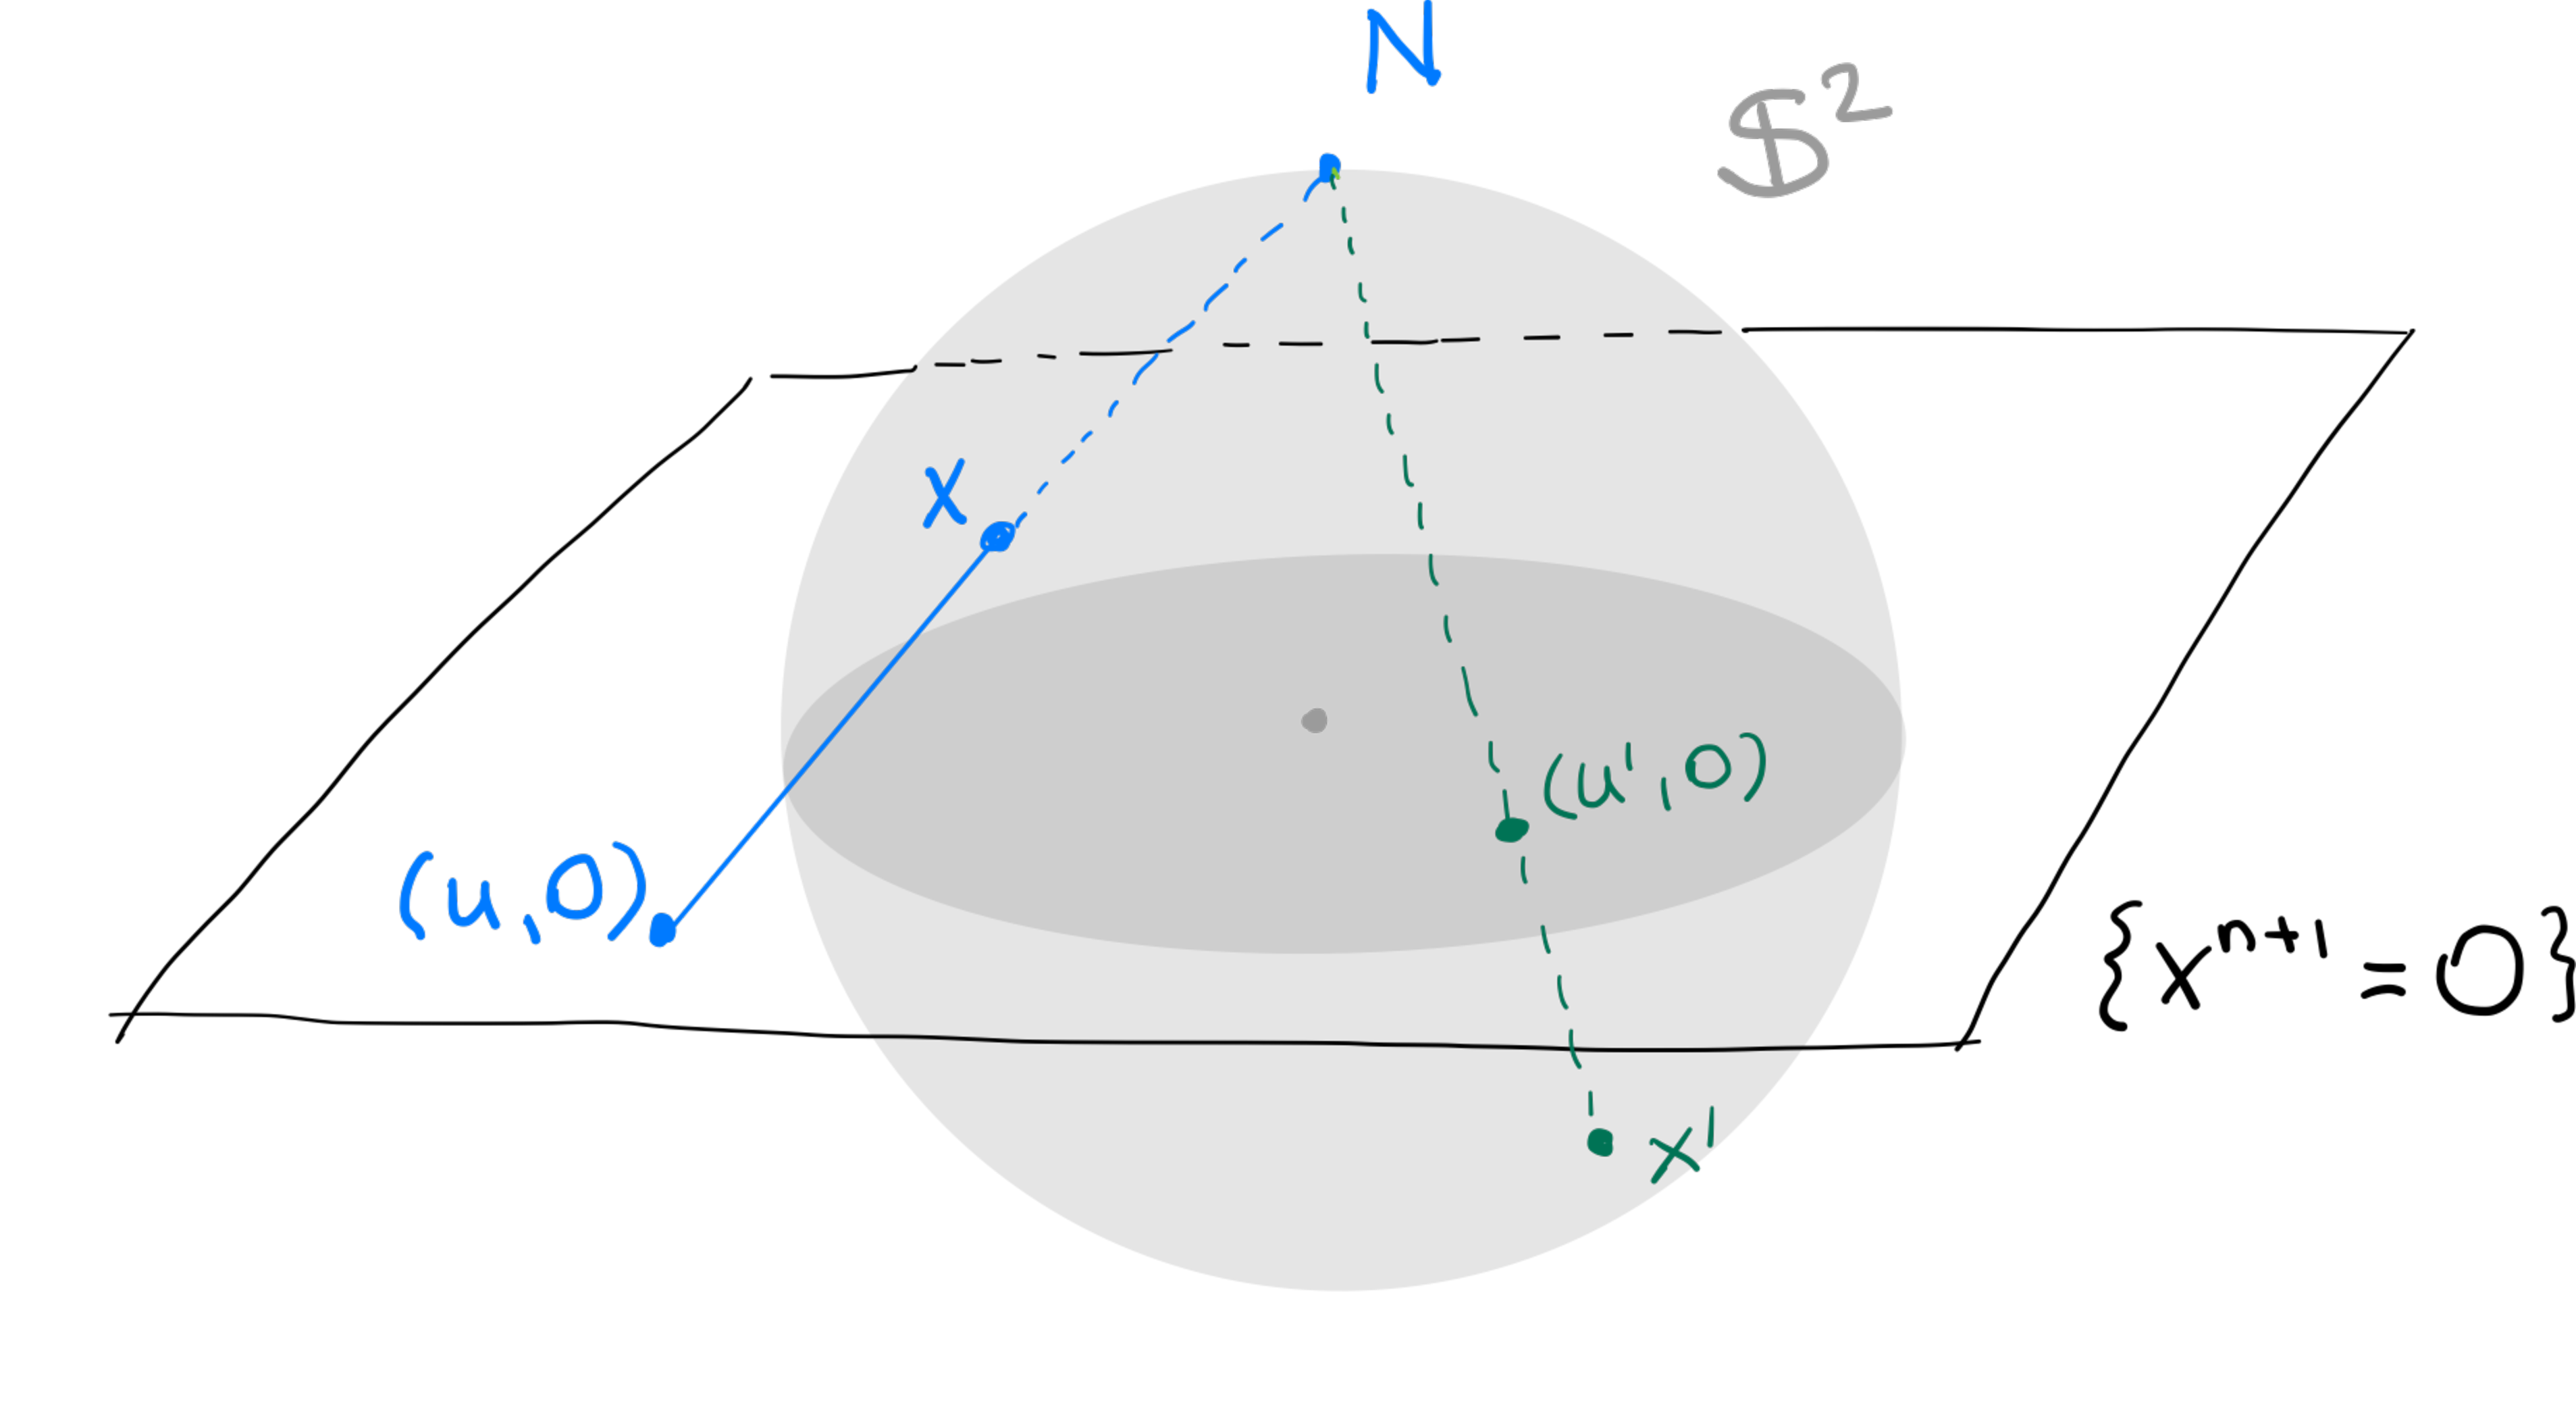
\includegraphics[trim=20pt 20pt 5pt 15pt,clip]{1_5_8-sphere}
  \end{marginfigure}
  \begin{equation}
    \sigma(x^1,\ldots,x^{n+1}) := \left(\frac{x^1}{1-x^{n+1}},\ldots,\frac{x^n}{1-x^{n+1}}\right),
  \end{equation}
  and $\widetilde\sigma:\bS^n\setminus\{S\}\to \R^n$, $\widetilde\sigma(x) := -\sigma(-x)$.
  \begin{enumerate}
    \item For any $x\in\bS^n\setminus\{N\}$, show that $\sigma(x)=u$ where $(u,0)$ is the point of intersection of the line passing through $N$ and $x$ with the hyperplane $\{x^{n+1}=0\}$.
      Similarly, show that $\widetilde\sigma(x)$ is the point where the line through $S$ and $x$ intersects the same hyperplane.
    \item Show that $\sigma$ is bijective and
      \begin{equation}
        \sigma^{-1}(u) = \left(\frac{2 u^1}{\|u\|^2+1}, \ldots,\frac{2 u^n}{\|u\|^2+1},\frac{\|u\|^2-1}{\|u\|^2+1}\right).
      \end{equation}
    \item Compute the transition map $\widetilde\sigma\circ\sigma^{-1}$ and verify that the atlas $\{(\bS^n\setminus\{N\},\sigma),(\bS^n\setminus\{S\},\widetilde\sigma)\}$ defines a smooth structure on $\bS^n$.
    \item Let $n=1$. Show that this smooth structure is the same as the one defined in Example~\ref{ex:S1emb}.
  \end{enumerate}
\end{exercise}

\begin{tcolorbox}
  The general definition of $C^r$-manifolds is mostly a matter of replacing occurrences of ``smooth'' in the text with $C^r$.
  The study of these more general structures is not dissimilar from what we will see in this course, with the exception of analytic and $C^0$-manifolds, but it introduces an unnecessary extra level of verbosity.
  In these notes we will only deal with smooth manifolds.
\end{tcolorbox}

\section{Smooth maps and differentiability}\label{sec:smoothfn}

With a well--defined differentiable structure and the idea of compatible charts, we have all the ingredients to lift the definition of differentiable maps from the euclidean world.

Before considering the general definition of a differentiable map, let's look at the simpler example of differentiable functions $f:M\to\R$ between a smooth manifold $M$ and $\R$.

\begin{marginfigure}
  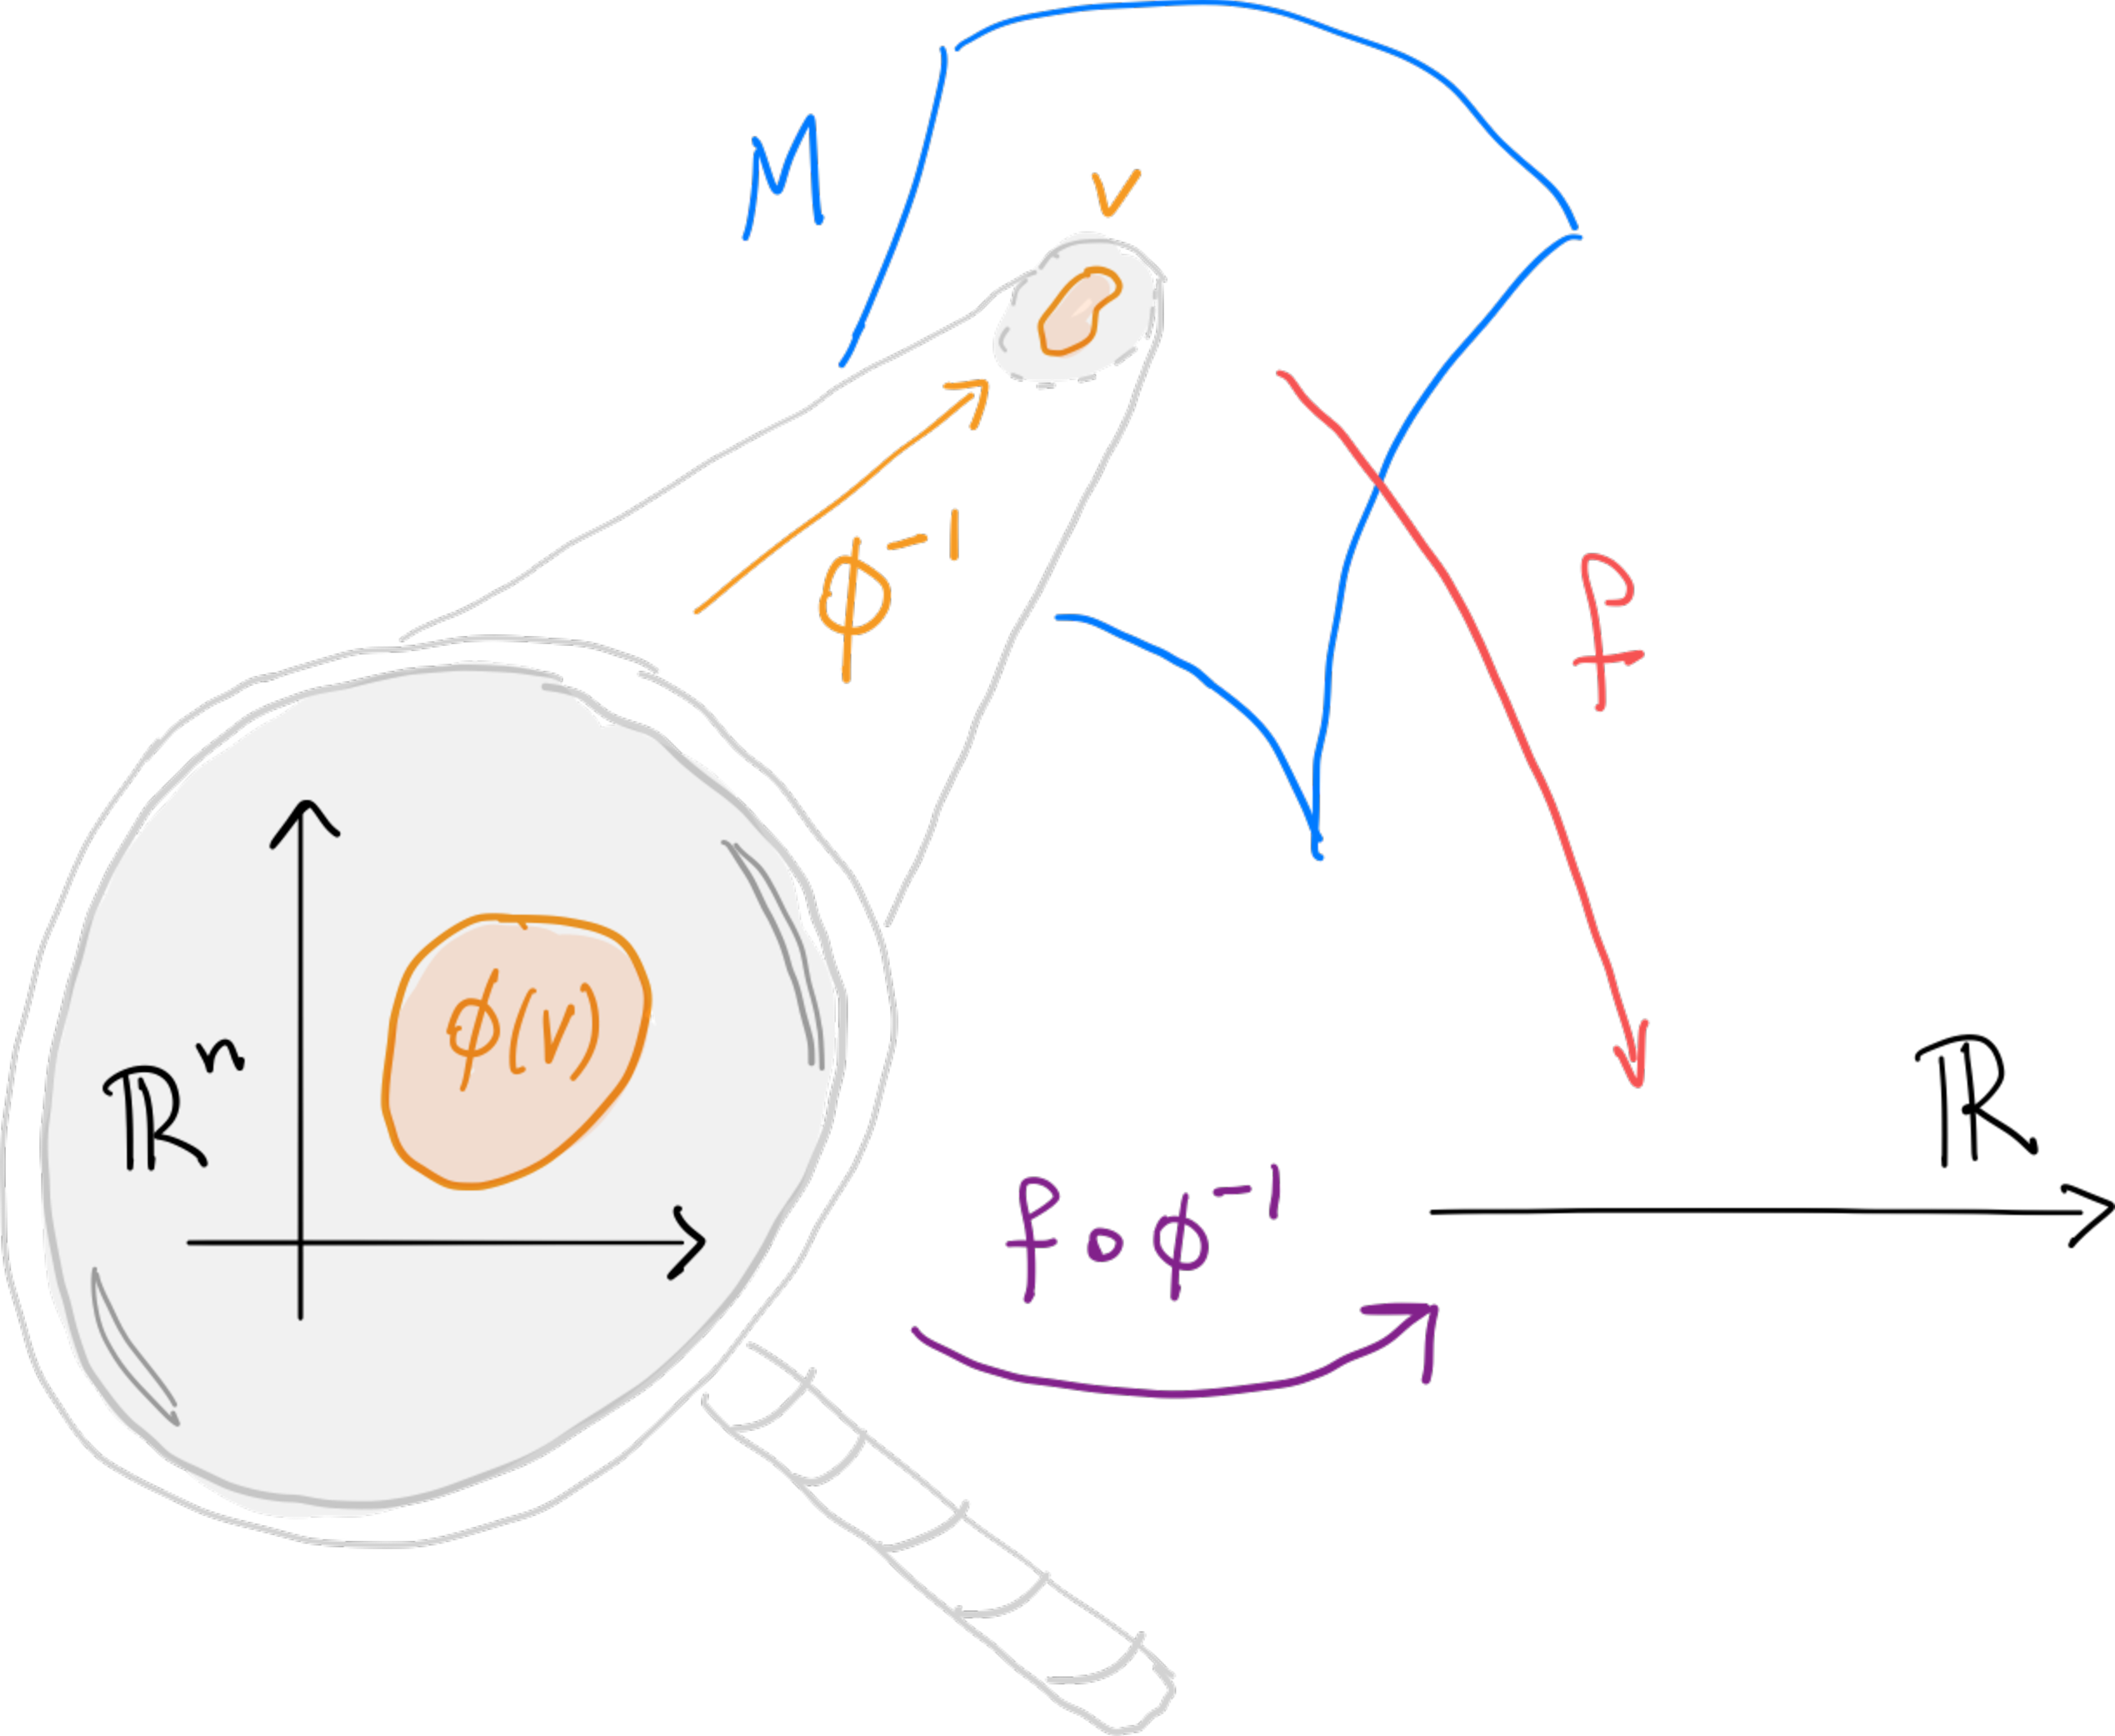
\includegraphics{1_5-diff-fun-v2.pdf}
  \label{fig:diff-fun}
  \caption{A function is differentiable if it is differentiable as a euclidean function through the magnifying lens provided by the charts.}
\end{marginfigure}
\begin{definition}
  A function $f:M\to\R$ from a smooth manifold $M$ of dimension $n$ to $\R$ is \emph{smooth}, or \emph{of class $C^\infty$}, if for any smooth chart $(\varphi, V)$ for $M$ the map $f\circ\varphi^{-1}:\varphi(V)\subset\R^n \to \R$ is smooth as a euclidean function on the open subset $\varphi(V)\subset\R^n$.
  We denote the space of smooth functions by $C^\infty(M)$.
\end{definition}

This, colloquially speaking, means that a function is differentiable if it is differentiable as a euclidean function through the magnifying lens (see Figure~\ref{fig:diff-fun}) provided by the charts.

\begin{exercise}
  Define the following operations on $C^\infty(M)$.
  For any $f,g\in C^\infty(M)$, $c\in\R$,
  \begin{equation}
    (f+g)(x) := f(x) + g(x),\quad
    (fg)(x) := f(x) g(x),\quad
    (cf)(x) := c f(x).
  \end{equation}
  Then, the space $C^\infty(M)$ endowed with the operations above is an \emph{algebra}\footnote{I.e. a vector space where you can also multiply two elements.} over $\R$.
\end{exercise}

The following theorem can be very convenient when you work with smooth functions.

\begin{proposition}
  Let $M$ be a smooth $n$-manifold and $f:M\to\R$ a real-valued function on $M$. Then, the following are equivalent:
  \begin{enumerate}[(i)]
    \item $f\in C^\infty(M)$;
    \item $M$ has an atlas $\cA$ such that for every chart $(U, \varphi)\in\cA$, $f\circ \varphi^{-1} : \R^n\supset\varphi(U)\to \R$ is $C^\infty$;
    \item for every point $p\in M$, there exists a smooth chart $(V,\psi)$ for $M$ such that $p\in V$ and the function $f\circ\psi^{-1} : \R^n\supset\psi(V)\to \R$ is $C^\infty$ on the open subset $\psi(V)\subset\R^n$.
  \end{enumerate}
\end{proposition}

\begin{exercise}
  Prove the proposition.\\
  \textit{\small Hint: go cyclic, for example show $(i)\Rightarrow(ii)$, $(ii)\Rightarrow(iii)$, $(iii)\Rightarrow(i)$.}
\end{exercise}

At this point, the generalization of smooth functions to smooth maps between manifolds should not come as a surprise.

\begin{definition}
  Let $F:M_1\to M_2$ be a continuous map \footnote{Remember: continuity is not a problem since $M_1$ and $M_2$ are topological spaces.} between two smooth manifolds of dimension $n_1$ and $n_2$ respectively.
  We say that $F$ is \emph{smooth}, or \emph{of class $C^\infty$}, if, for any chart $(\varphi_1, V_1)$ of $M_1$ and $(\varphi_2, V_2)$ of $M_2$, the map
  \begin{align}
    \varphi_2 \circ F \circ \varphi_1^{-1}: U_1 \to U_2,\qquad
    \begin{cases}
    U_1 := \varphi_1(V_1 \cap F^{-1}(V_2))\subset\R^{n_1}\\
    U_2 := \varphi_2(V_2)\subset\R^{n_2}
    \end{cases},
  \end{align}
  is smooth as a euclidean function.
  \marginnote[-6em]{Differently from your calculus classes, we are defining differentiability \emph{before} we define what the derivative is. Getting to it will require some amount of work, and will have to wait until the next chapter.}

  We denote by $C^\infty(M_1, M_2)$ the set of all functions $F:M_1\to M_2$ of class $C^\infty$.

  The map $\hat F := \varphi_2 \circ F \circ \varphi_1^{-1}$ is called the \emph{coordinate representation of $F$} with respect to the given coordinates.
\end{definition}

\begin{figure}[htp]
  \centering
  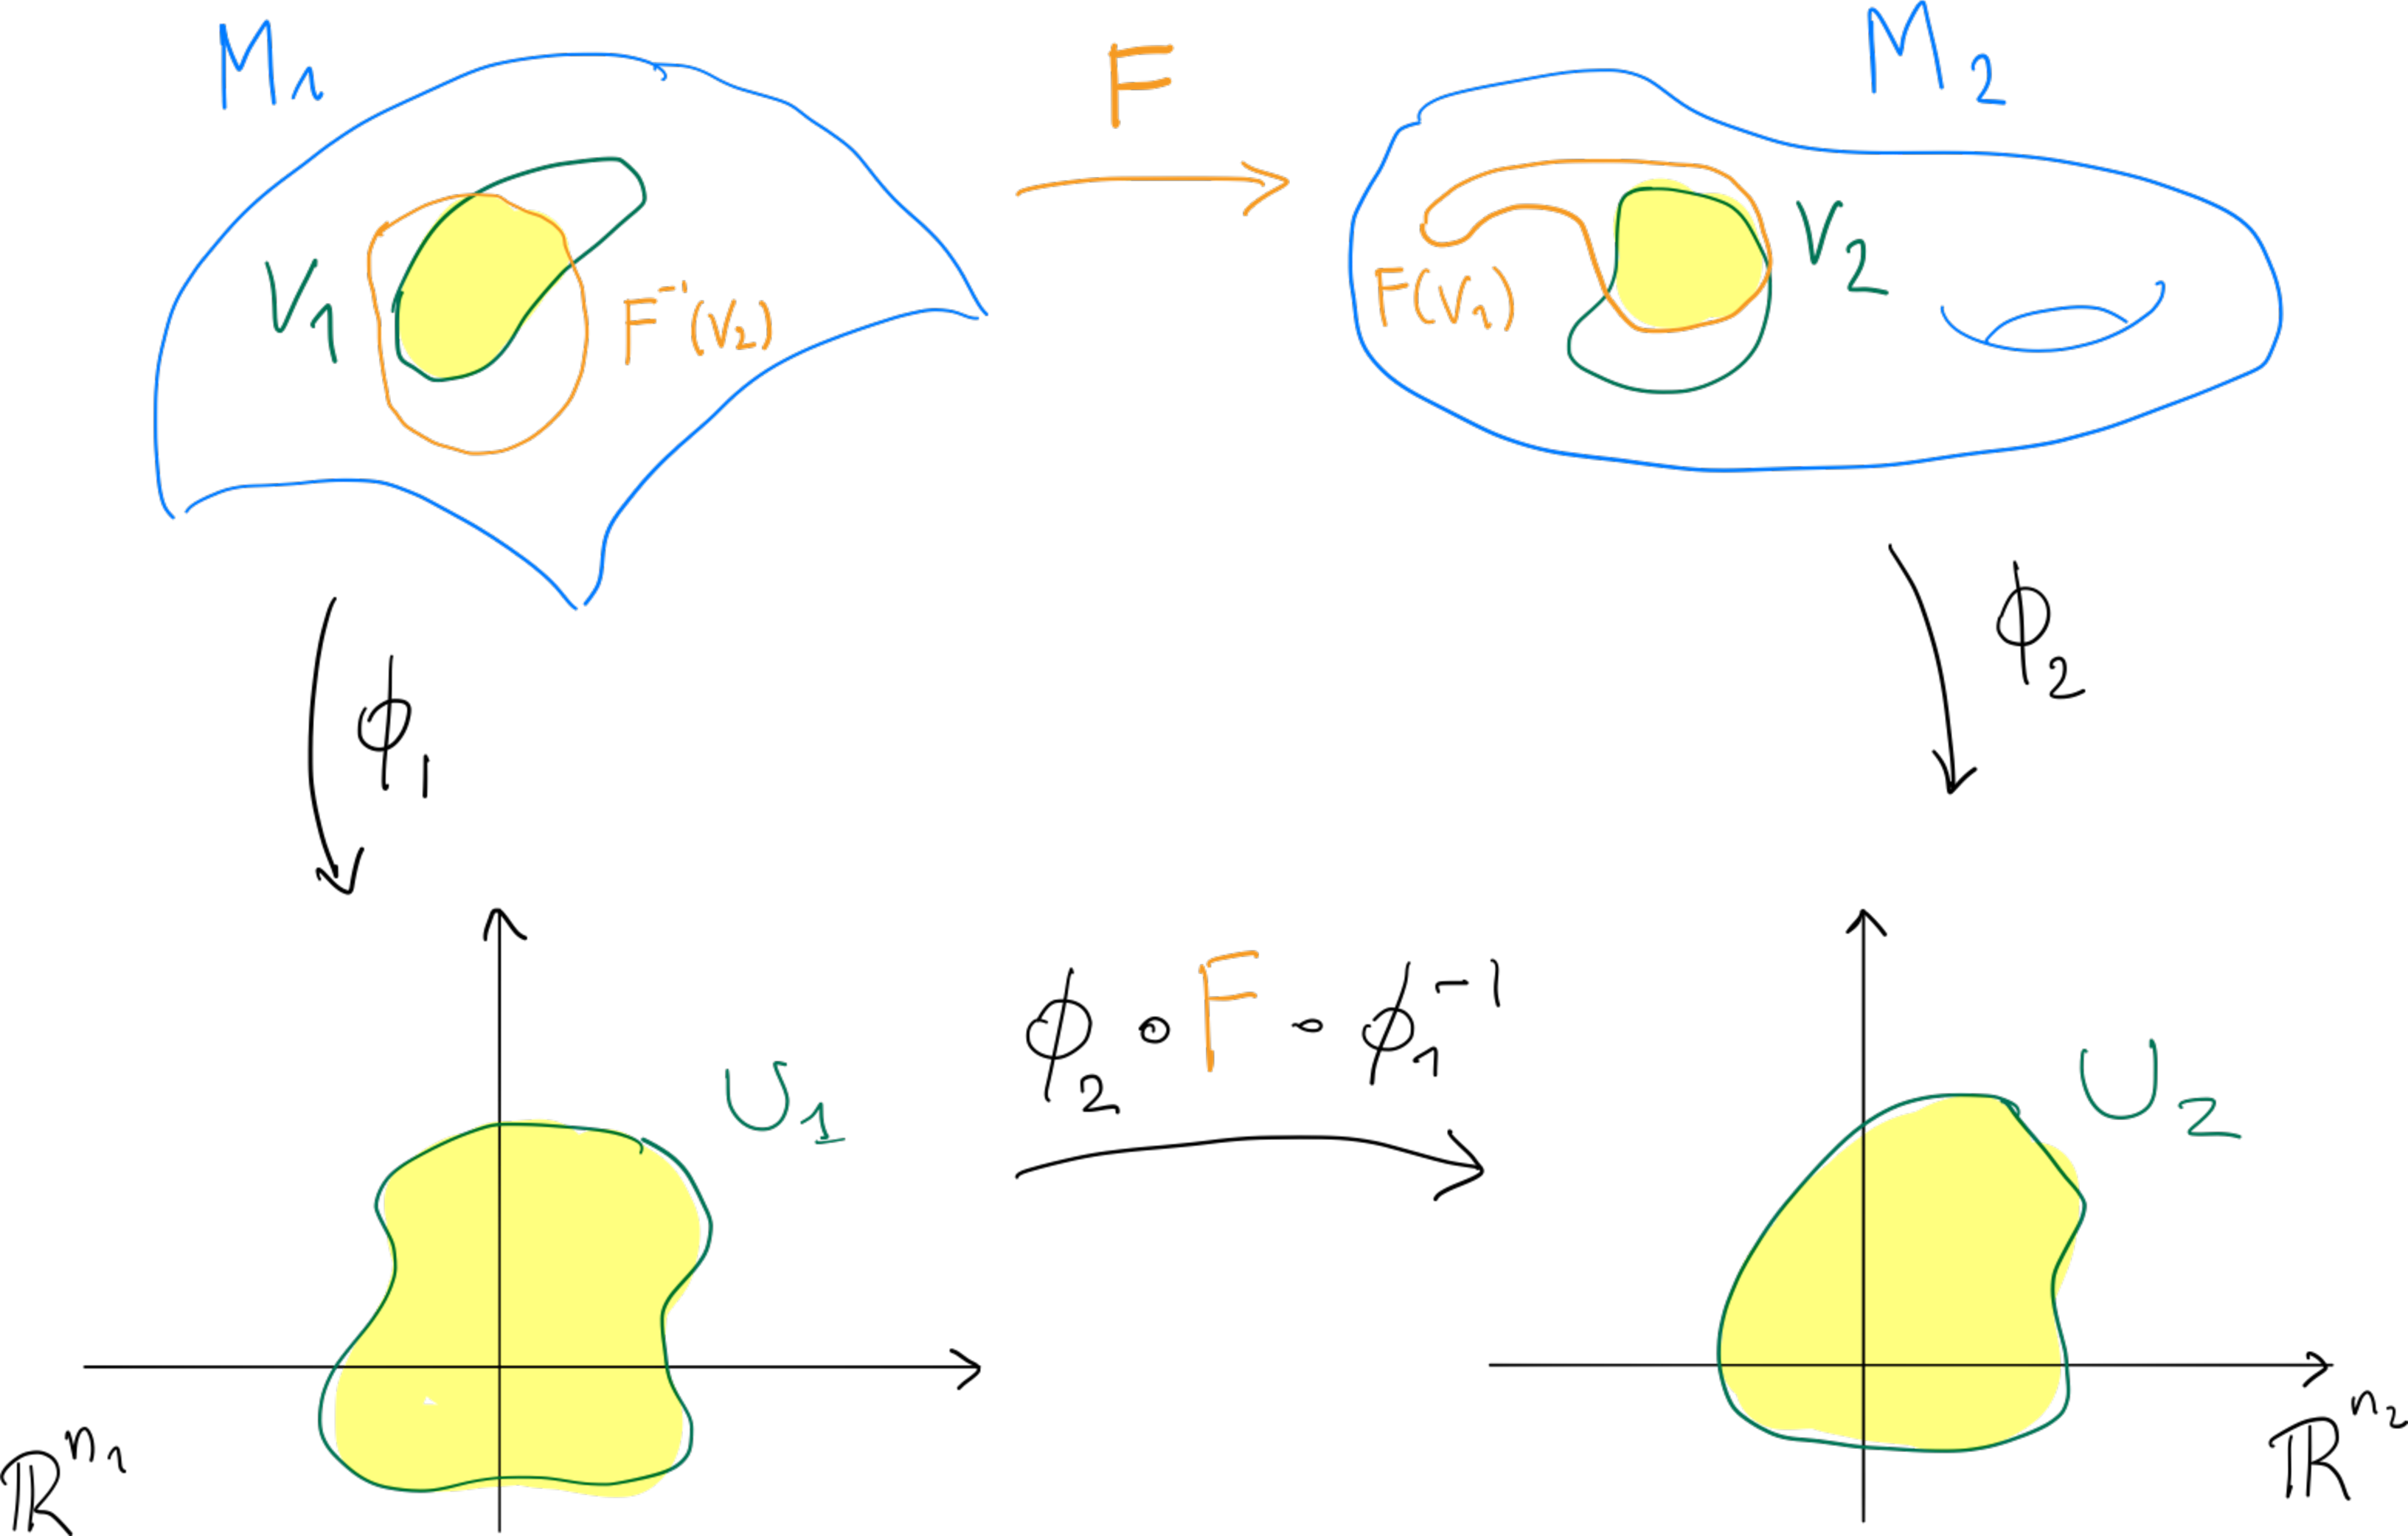
\includegraphics{1_3-diffble_maps.pdf}
  \caption{Maps are differentiable when they are differentiable as maps between euclidean spaces.}
  \label{fig:1.3-differentiable_maps}
\end{figure}

For a very simple and familiar example, consider the real valued function $f(x,y)= x^2+y^2$ defined on $\R^2$.
In polar coordinates on $U=\{(x,y)\in\R^2\mid x>0\}$, $f$ has the coordinate representation $\hat f (\rho, \theta) = \rho^2$.
Very often, where there is no ambiguity, we will simply identify $f$ and $\hat f$ and just write
\begin{quote}
  in the local coordinates $(\rho,\theta)$ on $U$, $f(\rho,\theta) = \rho^2$.
\end{quote}

A first observation about our definition of smooth maps is that, as one would hope, smoothness implies continuity.
%
\begin{exercise}
  Show that every smooth map is continuous.
\end{exercise}
%
\begin{exercise}
  Prove the following propositions, aiding your reasoning by drawing the relevant figures or commutative diagrams.
  \begin{proposition}
    Let $M$ be a smooth manifold of dimension $n$.
    Then $F:M\to\R^m$ is smooth iff for all smooth charts $(U,\varphi)$ of $M$, the function $F\circ\varphi^{-1}:\varphi(U)\to\R^m$ is smooth.
  \end{proposition}
  \begin{proposition}
    Let $M$ be a smooth manifold of dimension $n$.
    Then $F:\R^m\to M$ is smooth iff for all smooth charts $(U,\varphi)$ of $M$, the function $\varphi\circ F:F^{-1}(U)\to\R^n$ is smooth.
  \end{proposition}
  \begin{proposition}
    Let $M, N, P$ be three smooth manifolds, and suppose that $F:M\to N$ and $G:N\to P$ are smooth.
    Then $G\circ F\in C^\infty(M, P)$.
  \end{proposition}

  \begin{proposition}[Smoothness is a local property]\label{prop:smoothlocal}
    Let $F:M\to N$ be a continuous function and let $\{U_i\}_{i\in I}$ be an open cover for $M$. Then $F|_{U_i}:U_i \to N$ is smooth for every $i\in I$ iff $F:M\to N$ is smooth.
  \end{proposition}
\end{exercise}

It can be useful to know that there are alternative ways to characterize smooth functions.
\begin{exercise}[Equivalent definitions of smoothness]\label{prop:eq-def-smooth}
  Let $M_1$ and $M_2$ be smooth manifolds.
  Show that a map $F:M_1\to M_2$ is smooth if and only if either of the following conditions holds:
  \begin{enumerate}
    \item for every $p\in M_1$, there are smooth charts $(V_1,\phi_1)$, $p\in V_1$, and $(V_2,\phi_1)$, $F(p) \in V_2$, such that $F(V_1) \subseteq V_2$ and $\phi_2 \circ F \circ \phi_1^{-1}$ is smooth from $\phi_1(V_1)$ to $\phi_2(V_2)$;
    \item $F$ is continuous and there exists two smooth atlases $\{(V^1_\alpha, \phi^1_\alpha)\}$ and $\{(V^2_\beta, \phi^2_\beta)\}$, respectively for $M_1$ and $M_2$, such that for each $\alpha$ and $\beta$, $\phi^2_\beta \circ F \circ (\phi^1_\alpha)^{-1}$ is a smooth maph from $\phi^1_\alpha(V^1_\alpha \cap F(V_\beta^2))$ to $\phi^2_\beta(V^2_\beta)$.
  \end{enumerate}
\end{exercise}

\begin{definition}
  A \emph{diffeomorphism} $F$ between two smooth manifolds $M_1$ and $M_2$ is a bijective map such that $F\in C^\infty(M_1, M_2)$ and $F^{-1}\in C^\infty(M_2, M_1)$.
  %
  Two smooth manifolds $M_1$ and $M_2$ are called \emph{diffeomorphic} if there exists a diffeomorphism $F:M_1\to M_2$ between them.
\end{definition}

\begin{exercise}
  Any chart $(V, \varphi)$ of a manifold $M$ is a diffeomorphism between the manifolds $V\subset M$ and $\varphi(V)\subset\R^n$.
\end{exercise}

\begin{exercise}
  Prove that $\R^2\setminus\{(0,0)\}$ is a two-dimensional manifold and construct a diffeomorphism from this manifold to the circular cylinder
  \begin{equation}
    C := \{ (x,y,z)\in\R^3 \mid x^2+y^2 = 1\}\subset\R^3.
  \end{equation}
\end{exercise}

The following corollary is just a restatement of Proposition~\ref{prop:smoothlocal}, but provides a useful perspective on the construction of smooth maps.

\begin{proposition}[Gluing lemma for smooth maps]
  Let $M$ and $N$ be two smooth manifolds and let $\{U_\alpha\mid\alpha\in A\}$ be an open cover of $M$.
  Suppose that for each $\alpha\in A$ we are given a smooth map $F_
  \alpha:U_\alpha\to N$ such that the maps agree on the overlaps: $F_\alpha|_{U_\alpha\cap U_\beta} = F_\beta|_{U_\alpha\cap U_\beta}$ for all $\alpha,\beta\in A$. 
  Then there exists a unique smooth map $F:M\to N$ such that $F|_{U_\alpha} = F_\alpha$ for each $\alpha\in A$.
\end{proposition}

In other words, if you can define a map in a neighbourhood of each point in such a way that the locally defined maps all agree where they overlap, then the local definitions piece together to yield a global smooth map.
We will use this construction repeatedly throughout the course.
Sometimes, however, the local definitions are not guaranteed to agree. In this case one usually has to resort to a different tool: partitions of unity.
These allow to surgically patch objects together and make sure that they still have the required properties.
In the next section we will look more deeply into this.

\begin{tcolorbox}
  From now on, when we write manifold, chart, atlas, etc. we always mean smooth manifold, smooth chart, smooth atlas, etc..
\end{tcolorbox}

\begin{example}[A different smooth structure on $\R$]
  Consider the homeomorphism $\psi:\R\to\R$, $\psi(x) = x^3$.
  The atlas consisting of the global chart $(\R, \psi)$ defines a smooth structure on $\R$.
  This chart is not smoothly compatible with the standard smooth structure on $\R$ since $\id_\R \circ \psi^{-1} (y) = y^{1/3}$ is not smooth at $y=0$.
  Therefore, the smooth structure defined on $\R$ by $\psi$ is different from the standard one.
  You can adapt this idea to construct many different smooth structures on topological manifolds provided that they at least have one smooth structure.
\end{example}

\begin{exercise}
  Show that the smooth manifolds $(\R, \{(\R, \id_\R)\})$ and $(\R, \{(\R, \psi)\})$, defined using the smooth structures from the previous example, are diffeomorphic.
\end{exercise}

\begin{exercise}
  For $r>0$, let $\phi_r:\R\to\R$ be the map given by
  \begin{equation}
    \phi_r(t) := \begin{cases}
      t, & \mbox{if } t<0,\\
      rt, & \mbox{if } t\geq0.
    \end{cases}
  \end{equation}
  Let $\cA_r$ denote the maximal atlas on $\R$ containing the chart $(\R, \phi_r)$.
  \begin{enumerate}
    \item Show that the differentiable structures on $\R$ defined by $\cA_r$ and $\cA_s$, $0<r<s$, are different.
      This shows that there are uncountably many families of different differential structures on $\R$.
    \item Let $M_r$ be the manifold $\R$ equipped with the atlas $\cA_r$.
      Show that $M_r$ and $M_s$ are diffeomorphic for $r,s >0$.
  \end{enumerate}
\end{exercise}

\begin{remark}
  There exist examples of topological manifolds without smooth structures.
  It is also known that smooth manifolds of dimension $n < 4$ have exactly one smooth structure (up to diffeomorphisms) while ones of dimension $n > 4$ have finitely many\footnote{A beautiful example of this is the $7$-sphere $\bS^7$ which is known to have 28 non-diffeomorphic smooth structures.}.
  The case $n = 4$ is unknown: if you prove that there is only one smooth structure, you will have shown the smooth Poincar\'e conjecture.
\end{remark}

As a final exercise, we are going to relate smoothness of the maps with the smoothness of their components, which can be extremely useful when working in coordinates.

\begin{exercise}
  Let $F: M^m \to N^n$ be a continuous map between two manifolds. Then the following are equivalent:
  \marginnote{Recall Notation~\ref{ntn:coords}}
  \begin{enumerate}
    \item $F$ is smooth;
    \item $N$ has an atlas $\cA$ such that for all the charts $(V, \psi) = (V, y^1, \ldots, y^n)\in \cA$, the components $y^i \circ F: F^{-1}(V) \to \R$ of $F$ relative to the chart are all smooth;
    \item for every chat $(V, \psi) = (V, y^1, \ldots, y^n)$ on $N$, the components $y^i \circ F: F^{-1}(V) \to \R$ of $F$ relative to the chart are all smooth.
  \end{enumerate}
  Note that this, in particular, holds for $N=\R^n$.
\end{exercise}

\section{Partitions of unity}

\newthought{Cutoff functions} are a class of smooth functions that will be of crucial importance throughout the course, and whose existence cannot be given for granted.
Since their definition and construction does not require more than what we have just seen, let's talk about them now.

First of all, recall that the \emph{support} of a smooth function $f: M \to \R$, denoted by $\supp(f)$, is defined as
\marginnote[2em]{The bar over the set denotes its closure.}
\begin{equation}
  \supp(f) := \overline{\{ p\in M \;\mid\; f(p) \neq 0\}}.
\end{equation}

We will introduce those functions with a proposition, and will spend the rest of this chapter proving it.

\begin{figure}[htp!]
  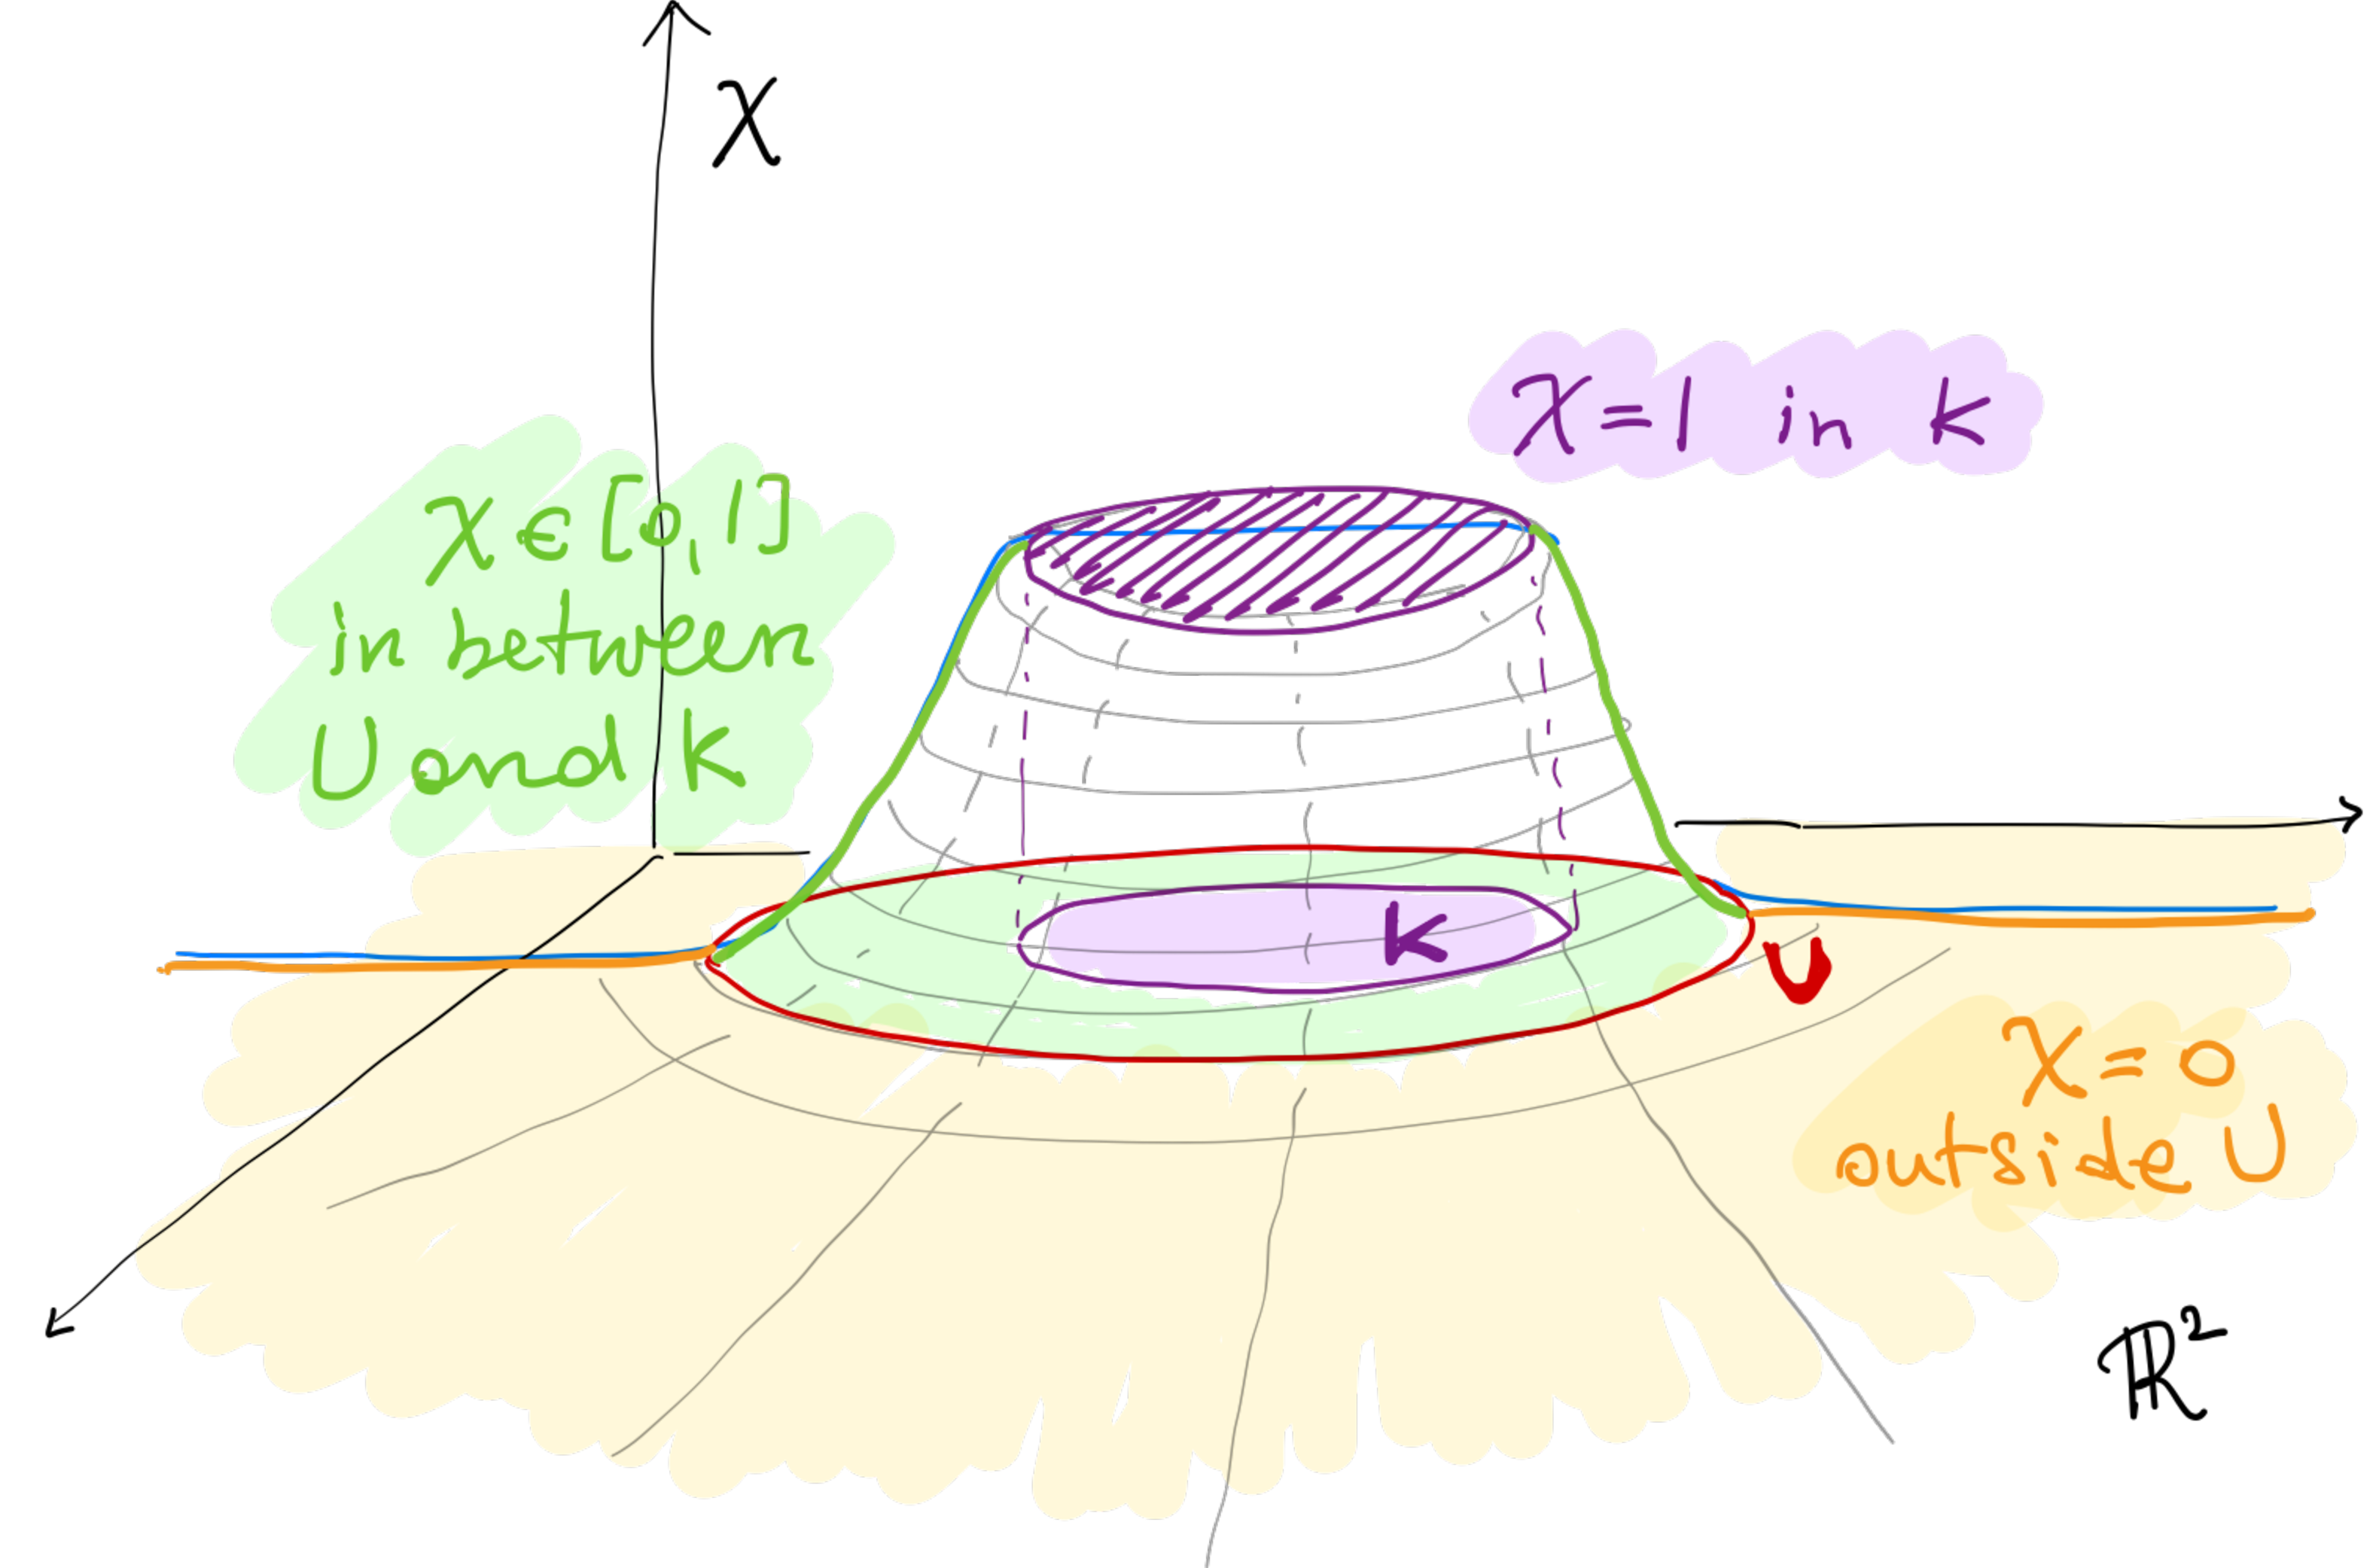
\includegraphics{1_6-cutoffs.pdf}
\end{figure}

\begin{proposition}[Cutoff functions]\label{prop:cutoff}
  Let $M$ be a smooth manifold and $K\subset U\subset M$ two subsets such that $K$ is closed and $U$ is open.
  Then, there exists a smooth function $\chi: M \to\R$, called \emph{cutoff} function, with the following properties
  \begin{enumerate}[(i)]
    \item $0 \leq \chi \leq 1$ for all $p\in M$;
    \item $\supp(\chi)\subset U$;
    \item $\chi(p) = 1$ for all $p\in K$.
  \end{enumerate}
\end{proposition}

The proof of this proposition involves a general result which is quite technical and whose proof will be omitted.
You can refer to~\cite{book:lee, book:tu} if you are curious to see the details.

Instead, we will show a special case of Proposition~\ref{prop:cutoff}. The main reason is that it involves an explicit construction of the cutoff which can be convenient to have at hand later on.

\begin{lemma}[Cutoff functions, compact case]
  Let $M$ be a smooth manifold and $K\subset U\subset M$ two subsets such that $K$ is compact and $U$ is open.
  Then, there exists a smooth function $\chi: M \to\R$ with the following properties
  \begin{enumerate}[(i)]
    \item $0 \leq \chi \leq 1$ for all $p\in M$;
    \item $\supp(\chi)\subset U$;
    \item $\chi(p) = 1$ for all $p\in K$.
  \end{enumerate}
\end{lemma}
\begin{proof}
  \newthought{Part 1}.
  To warm up, let's do some first year analysis.
  For any pair of real numbers $r < R$ there exists a smooth function $f: \R \to [0,1]$ such that $f(t) = 1$ for $t \leq r$, $f(t) = 0$ for $t \geq R$ and $0<f(t)<1$ for $t\in(r,R)$.

  We can construct this explicitly by means of the function
  \begin{equation}
    h:\R\to\R, \quad h(t):= \begin{cases}
      e^{-1/t}, & t>0,\\
      0, & t \leq 0.
    \end{cases}
  \end{equation}

  \begin{exercise}
    Prove by induction that for $t>0$ and $k\geq 0$, the $k$th derivative $h^{(k)}(t)$ is of the form $p_{2k}(1/t)e^{-1/t}$ for some polynomial $p_{2k}(x)$ of degree $2k$ in $x$.
    Use this to show that $h\in C^\infty(\R)$ and that $h^{(k)}(0) = 0$ for all $k\geq 0$.
  \end{exercise}

  The function $f$ that we are seeking is then\footnote{Exercise: check that such function $f$ satisfies all the desired properties.} given by
  \begin{equation}
    f(t) := \frac{h(R-t)}{h(R-t) + h(t-r)}.
  \end{equation}

  \newthought{Part 2}.
  Let's extend $f$ to $\R^n$.
  Denote $B_r \subset \R^n$ the open ball of radius $r$ around the origin.
  Then, for any $0 < r < R$ we seek a function $g:\R^n\to\R$ such that $g(x) = 1$ for all $x\in \overline{B_r}$, $g(x) = 0$ for all $x\in \R^n\setminus B_R$ and $0< g(x)< 1$ for all $x\in B_R\setminus\overline{B_r}$.
  This is immediately achieved by defining $g(x) := f(\|x\|)$, where $f$ is the function defined in the previous step.

  \newthought{Part 3}.
  Let's now pick a point $p\in M$ and an arbitrary neighbourhood $U$ of $p$. Choosing an appropriate chart about $p$, the previous step implies that we can choose a smaller neighbourhood $V\subset U$ of $p$ with $\overline V\subset U$ and such that there exists a smooth function $\chi: M \to [0,1]$ satisfying $\chi(p) = 1$ for all $p\in\overline{V}$ and $\chi(p) = 0$ for all $p\in M\setminus U$.

  \newthought{Part 4}.
  We are ready to complete the proof.
  For each point $p\in K$, choose two neighbourhoods $V_p \subset U_p$ such that $\overline{V_p}\subset K$ and $U_p \subset U$.
  Since $K$ is compact, it admits a finite cover in terms of these sets: i.e. there are finitely many points $p_1, \ldots, p_N \in K$ such that $K \subset \bigcup_{i=1}^N V_{p_i}$.
  For each $i$, choose $\chi_i: M \to [0,1]$ as in the previous step: $\chi_i(p) = 1$ for all $p\in\overline{V_{p_i}}$ and $\chi_i(p) = 0$ for all $p\in M\setminus U_{p_i}$.
  The proof is completed by defining
  \begin{equation}
    \chi := 1 - \prod_{i=1}^N(1 - \chi_i(p)).
  \end{equation}
\end{proof}

We are not there yet. To extend this result to our needs will need a new tool, which will be useful throughout the course and in many courses to come.

\begin{definition}
  Let $M$ be a smooth manifold. A \emph{partition of unity} is a collection $\{\rho_\alpha \mid \alpha\in A\}$ of functions $\rho_\alpha:M\to\R$ such that
  \begin{enumerate}[(i)]
    \item $0 \leq \rho_\alpha \leq 1$ for all $p\in M$ and $\alpha\in A$;
    \item\label{def:pou.2} the collection $\{\rho_\alpha \mid \alpha\in A\}$ is \emph{locally finite}, that is, for any $p\in M$ there are at most finitely many $\alpha\in A$ such that $p\in\supp(\rho_\alpha)$;
    \item for all $p\in M$ one has $\sum_{\alpha\in A} \rho_\alpha(p) = 1$.
      \marginnote{For any $p$, $\sum_{\alpha\in A} \rho_\alpha(p)$ is a finite sum by~\ref{def:pou.2}. Thus, the function defined by the sum $\rho := \sum \rho_\alpha$ is a well define smooth function on $M$. We call such sum a \emph{locally finite} sum.}
  \end{enumerate}
\end{definition}

\begin{remark}
  Note that the existence of a partition of unity is a distinguished feature of differentiable manifolds: stronger structures, like analytic or holomorphic ones, in general fail to have one.
\end{remark}

Throughout the course we will be mostly interested in partitions of unity $\{\rho_\alpha \mid \alpha\in A\}$ which are \emph{subordinate} to an open cover $\{U_\alpha\mid\alpha\in A\}$, that is, such that $\supp_\alpha(\rho_\alpha) \subset U_\alpha$ for each $\alpha\in A$.

\begin{theorem}\label{thm:partitionof1}
  \marginnote[1.5em]{We are going to omit the proof of this theorem, for its details you can refer to~\cite[Proposition 13.6]{book:tu} or~\cite[Theorem 2.23]{book:lee}.}
  Let $M$ be a smooth manifold. For any open cover $\{U_\alpha\mid\alpha\in A\}$ of $M$, there exists a partition of unity $\{\rho_\alpha \mid \alpha\in A\}$ subordinate to $\{U_\alpha\mid\alpha\in A\}$.
\end{theorem}

With this result at hand, Proposition~\ref{prop:cutoff} can be shown very easily.

\begin{proof}[Proof of Proposition~\ref{prop:cutoff}.]
  Consider the open cover of $M$ given by $\cC:=\{M\setminus K, U\}$.
  Then Theorem~\ref{thm:partitionof1} implies that there exists a partition of unity $\{\rho_U, \rho_{M\setminus K}\}$ adapted to $\cC$. The function $\chi := \rho_U$ is our cutoff function.
\end{proof}

\section{Manifolds with boundary}\label{sec:mbnd}

\newthought{The definition of manifolds has a serious limitation}, even though it is perfectly good to describe curves\footnote{E.g. the circle seen in Example~\ref{ex:S1emb}.} and surfaces\footnote{E.g. the $2$-spheres $\bS^2$.}, it fails to describe many natural objects like a \emph{closed} interval $[a,b]\in\R$ or the \emph{closed} disk $D_1(0)$ of Example~\ref{ex:uball}.
Note that in each of these cases, both the interior and the boundary are smooth manifolds and their dimension differ by one\footnote{In the first case the interior $(a,b)$ is a $1$-manifold and the boundary, the set $\partial[a,b] = \{a,b\}$, is a $0$-manifold. In the second case the interior of $D_1(0)$ is the open unit ball, a $2$-manifold, and the boundary $\partial D_1(0)$ is the $1$-manifold $\bS^1$.}.

Let's do a step back and think about topological manifolds: since both the closed interval and the closed disk are closed sets, we have problems to make them locally euclidean in neighbourhoods of their boundaries.
Can we modify our local model to resemble something with a boundary?

Of course this is a rhetorical question.
We can generalize our definition by considering the \emph{closed upper half-spaces}
\begin{marginfigure}[2em]
  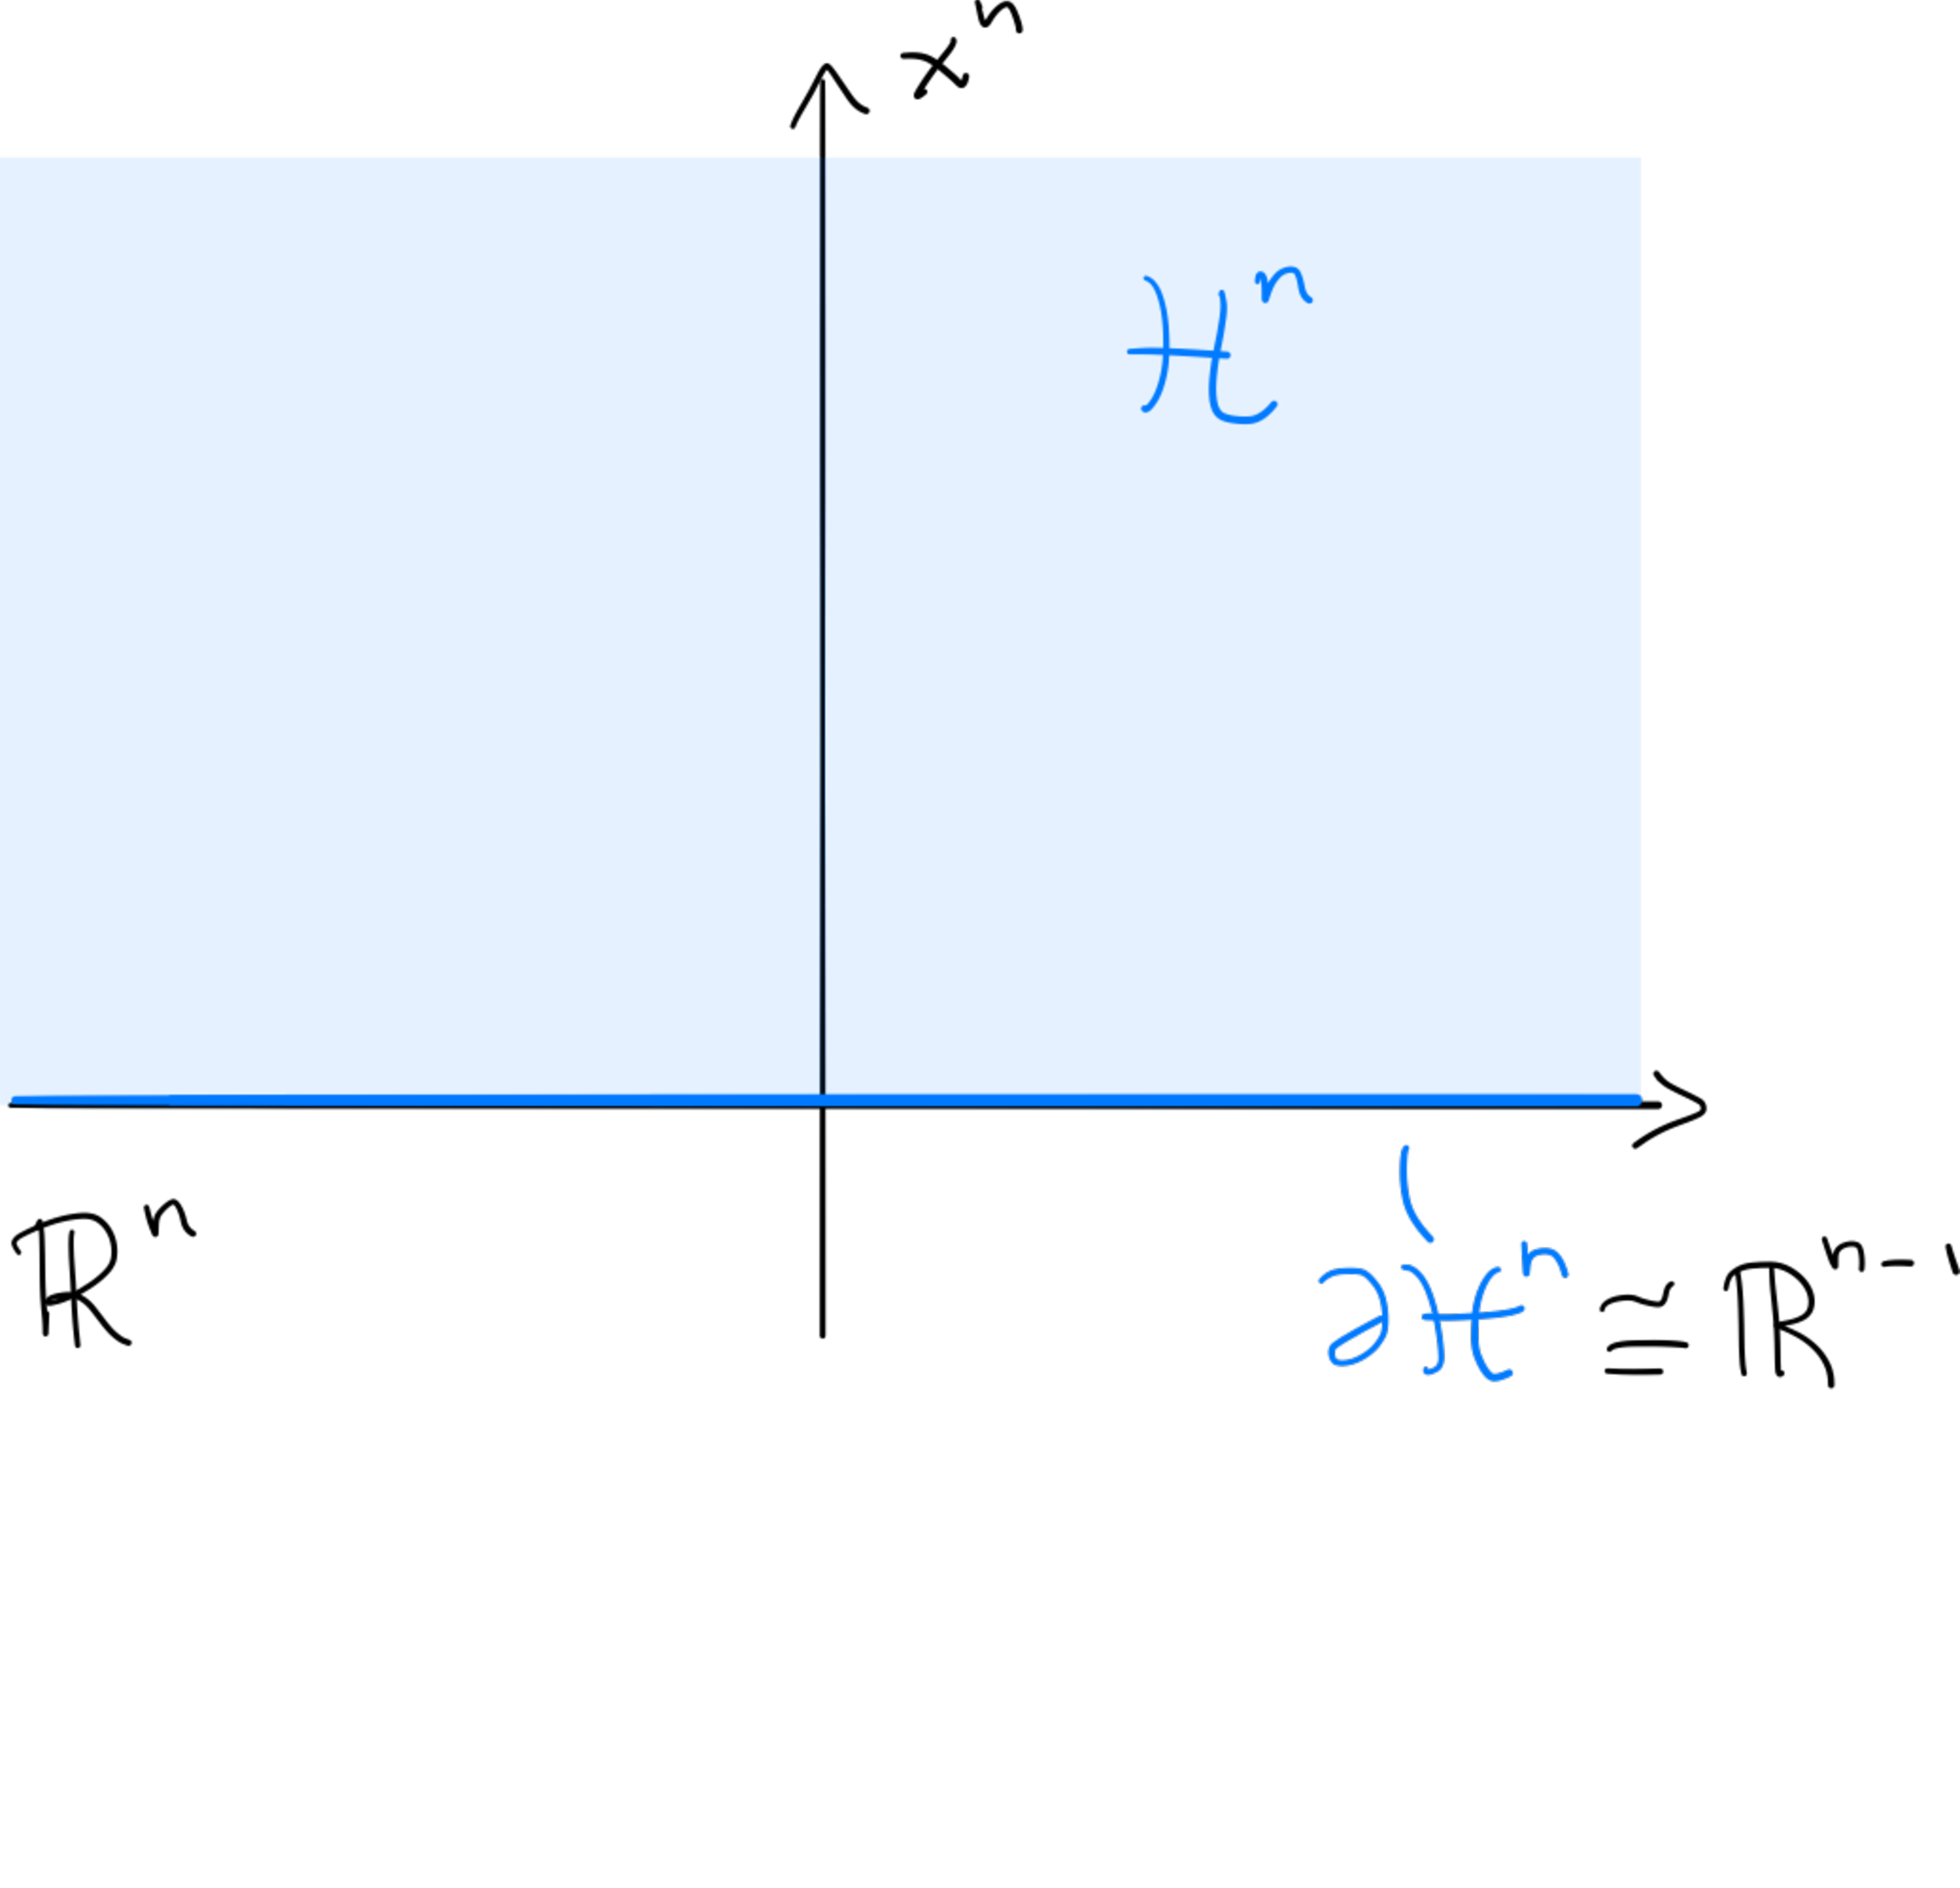
\includegraphics{1_4-upper_space.pdf}
\end{marginfigure}
\begin{equation}
  \cH^n = \{x=(x^1, \ldots, x^n)\in\R^n\mid x^n \geq 0\},
\end{equation}
with its $(n-1)$-dimensional boundary
\begin{equation}
  \partial\cH^n = \{x=(x^1, \ldots, x^n)\in\R^n\mid x^n = 0\}
\end{equation}
and the topology inherited by $\R^n$, as a replacement for our local model $\R^n$.

\begin{definition}
  A topological space $M$ is a \emph{topological manifold with boundary} of dimension $n$, or topological $n$-manifold with boundary, if it has the following properties
  \begin{enumerate}[(i)]
    \item $M$ is a Hausdorff space;
    \item $M$ is second countable;
    \item $M$ is \emph{locally homeomorphic to $\cH^n$}, any point $x\in M$ has a neighbourhood that is homeomorphic to a (relatively) open\footnote{Recall that $U\subset\cH^n$ is relatively open, that is open with respect to the relative topology, if there exist an open set $\widetilde U\subset\R^n$ such that $U = \widetilde U \cap \cH^n$.} subset of $\cH^n$.
  \end{enumerate}

  A \emph{chart} on $M$ is a pair $(U, \varphi)$ consisting of an open set $U\subset M$ and a homeomorphism $\varphi: U \to \varphi(U)\subset \cH^n$.
\end{definition}

\begin{figure}
  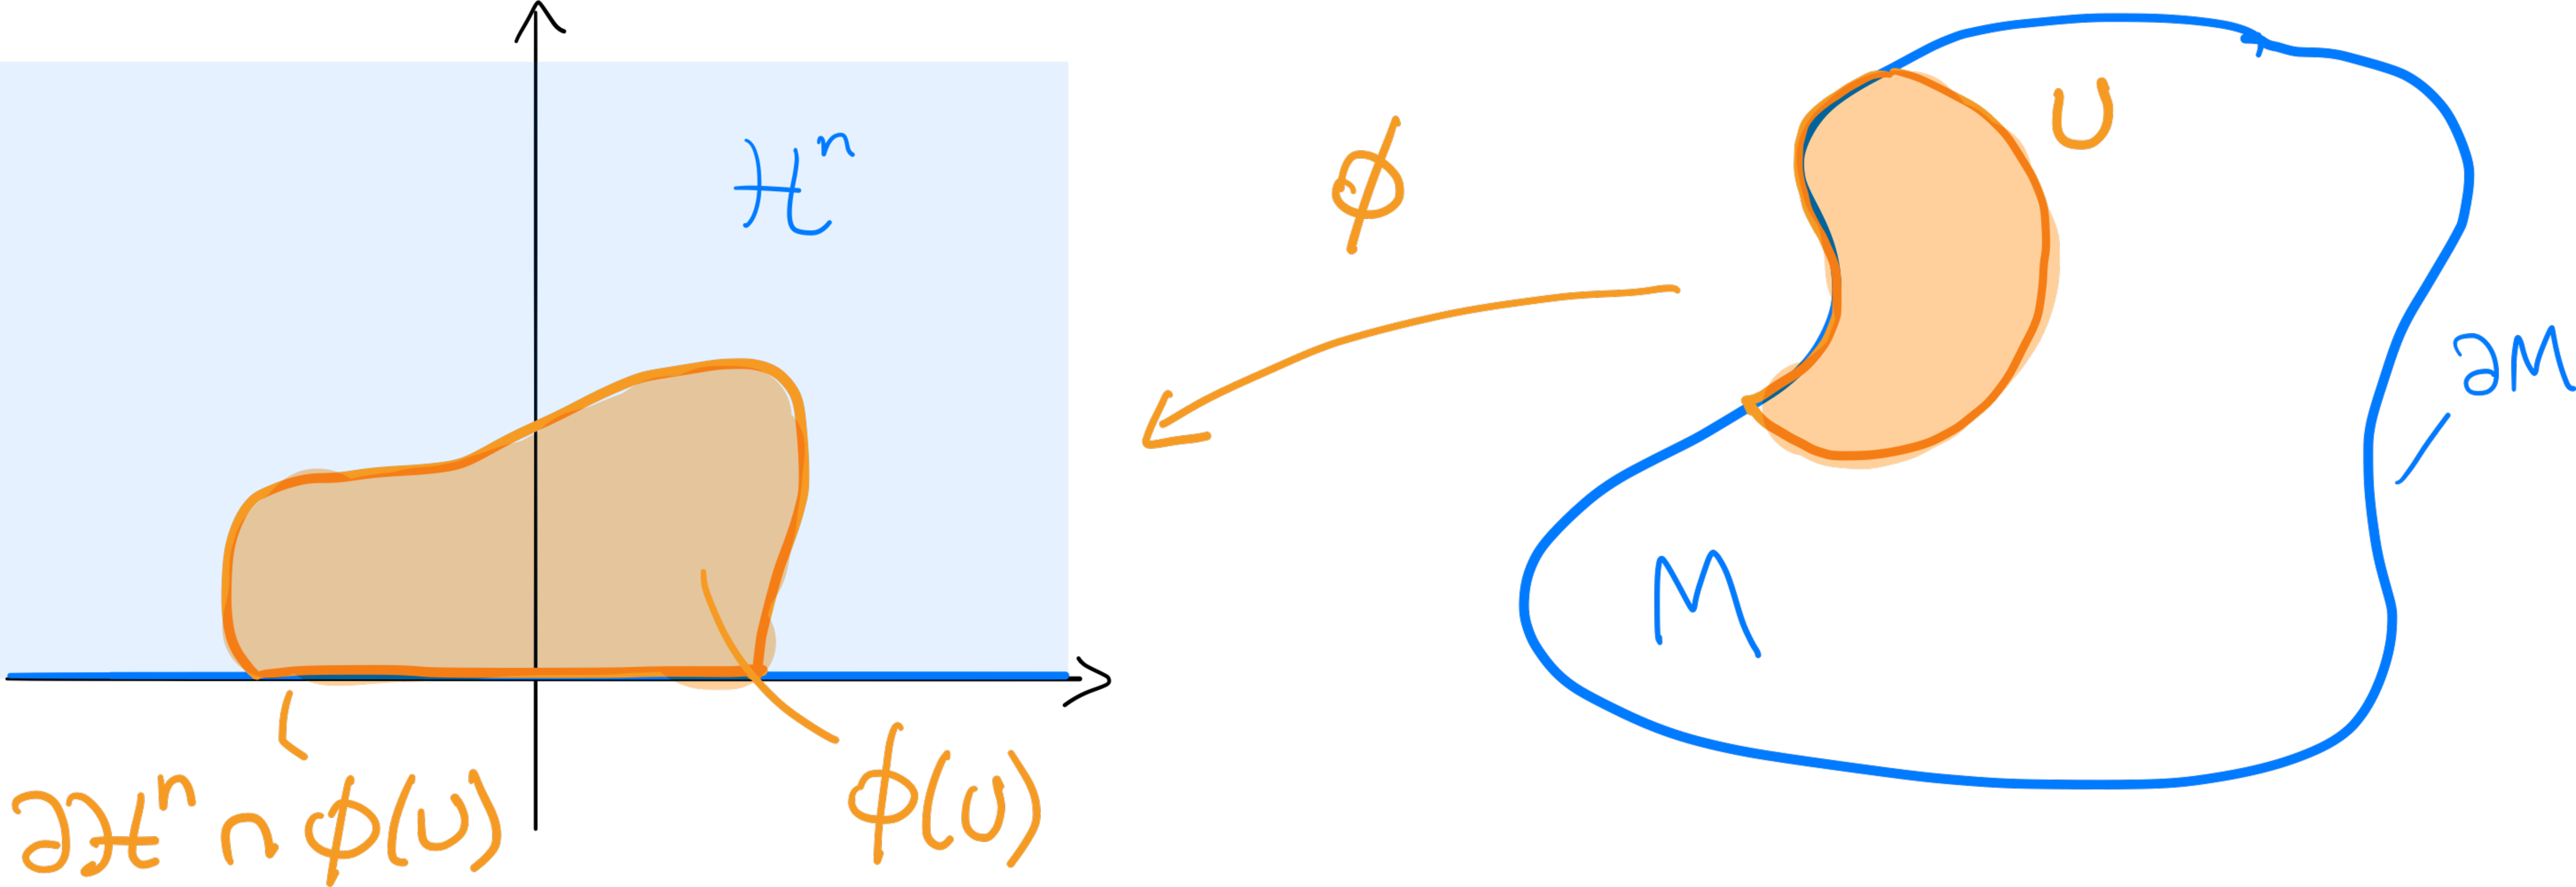
\includegraphics{1_4-mfld-w-bdry.pdf}
\end{figure}

\begin{example}\label{ex:mobius}
  A M\"obius strip $M$ is a connected $2$-manifold with boundary.
  As a topological space it is the quotient\footnote{Think of a strip of paper whose ends have been glued with a twist.} $\R\times[0,1]$ via the identification $(x,y)\sim(x+1, 1-y)$.
  The projection $\pi: [(x,y)] \mapsto (\cos(2\pi x), \sin(2\pi x))$ is a continuous surjective map to $\bS^1$.
  Given $x_0\in\R$, we can choose charts $[(x,y)]\mapsto (e^x\cos(\pi y), e^x\sin(\pi y))$ for $x\in(x_0 - \epsilon, x_0 + \epsilon)$ and any $\epsilon < 1/2$.
  \marginnote{Note that $\partial M$ is diffeomorphic to $\bS^1$. In fact, this is actually an example of a non-trivial fiber bundle, something that will make sense only a few chapters from now.
  In this case, $M$ is a bundle of intervals over a circle.}
\end{example}

We saw in Proposition~\ref{prop:uniqdiffeoinclusion} that differentiability is a local property, which means that is a property defined on open sets.
To clarify what it means to have differentiable structures on manifolds with boundary, we will thus need to clarify what it means for a function defined on $\cH^n$ to be differentiable at points on $\partial\cH^n$.
As it turns out, this is a minor modification of our previous definition that stems directly from the definition of the induced topology.

\begin{definition}
  Let $U\subset\cH^n$ be a relatively open set. A map $f: U\to\R^m$ is \emph{$r$-times continuously differentiable}, or of class $C^r$, if there exists an open set $\widetilde U\in\R^n$ and a map $\widetilde f\in C^r(\widetilde U, \R^m)$ such that $U\subset\widetilde U$ and $\widetilde f|_U = f$.
  The function $f$ is said to be \emph{smooth}, or of class $C^\infty$, if $f$ is $r$-times continuously differentiable for all $r\geq 1$.
\end{definition}

With such definition at hand, one can define compatibility, smooth atlases and differentiable structures as in Definition~\ref{def:crcomp}, Definition~\ref{def:cratlas} and Definition~\ref{def:diffstr} by considering charts taking value in $\cH^n$.

\begin{exercise}
  Explicitly state the definitions above in the case of manifolds with boundary.
\end{exercise}

\begin{definition}\label{def:diffmanifoldwb}
  \marginnote{Remember that the differentiable structure is an equivalence class of smooth atlases.}
  A \emph{smooth manifold with boundary} of dimension $n$ is a pair $(M, \cA)$ of a topological $n$-manifold with boundary $M$ and a smooth differentiable structure $\cA = \{(U_\alpha, \varphi_\alpha) \mid \alpha\in A\}$ on $M$.

  \marginnote{The boundary $\partial M$ as defined by~\eqref{def:bdry} can differ from its topological boundary as a subset of another topological space. For example the boundary $\partial\bS^1$ of the circle as a manifold is empty, but the boundary of the circle $\bS^1$ as a subset of $\R^2$ is $\bS^1$ itself.}
  The \emph{boundary} of $M$ is defined as
  \begin{equation}\label{def:bdry}
    \partial M := \bigcup_{\alpha\in A} \varphi_\alpha^{-1}\left(\varphi_\alpha(V_\alpha)\cap \partial\cH^n\right).
  \end{equation}
\end{definition}

\begin{proposition}\label{prop:bdwelldef}
  The boundary $\partial M$ is well--defined\footnote{In the sense that smooth charts send boundary pieces to boundary pieces. Note that the definition of the boundary holds for topological manifolds as well, but showing that it is well--defined is much more complicated and will be omitted.}.
\end{proposition}
\begin{proof}
  The statement follows if we show that the transition maps send boundary pieces to boundary pieces.
  It turns out that this fact is more general: for any diffeomorphism $f:U \to V$, where $U,V \subset\cH^n$ are relatively open, it holds that $x\in U\cap\partial\cH^n$ if and only if $f(x)\in V\cap\partial\cH^n$.

  Indeed, let $x\in U\cap(\cH^n\setminus\partial\cH^n)$ be a point in the interior of $U$. Expanding $f$ in Taylor series up to the first order, we have
  \begin{equation}
    f(x+h) = f(x) + Df|_x h + O(\|h\|).
  \end{equation}
  Since the total derivative $D f$ at $x$ is an isomorphism, there exist an open neighbourhood $\cO$ of $x$ such that $f(\cO)$ is open in $\R^n$ and thus $f(x)\in V\cap(\cH^n\setminus\partial\cH^n)$.
\end{proof}

\begin{remark}
  The definition of smooth maps and the propositions proven in Section~\ref{sec:smoothfn} all hold also in the case of smooth manifolds with boundary. 
\end{remark}

\begin{example}\label{ex:mfldbdryinterval}
  Let's go back to the closed interval $M=[a,b]\subset\R$. 
  With the atlas
  \begin{equation}
    \cA=\big\{
      \big([a,b), \; x\mapsto x-a\big),
      \big((a,b], \; x\mapsto b-x\big)
    \big\}
  \end{equation}
  it is a differentiable $1$-manifold with boundary $\partial M = \{a\} \cup \{b\} = \{a, b\}$.
\end{example}

Let's go back to our observation at the beginning of this section.
We started by observing that some objects seemed to be the ``sum'' of a boundary manifold and an interior manifold.
Can we make sense of such observation using our newly introduced definition?

\begin{proposition}
  Let $M$ be a differentiable $n$-manifold with boundary.
  Then $\mathring M := M\setminus\partial M$ and $\partial M$ inherit the structure of manifolds (without boundary) of dimensions $\dim(\mathring M)=n$ and $\dim(\partial M) = n-1$.
\end{proposition}
\begin{proof}
  Let $\cA = \{(U_\alpha,\varphi_\alpha) \mid \alpha\in A\}$ be an atlas for $M$. 
  Then
  \begin{equation}
    \cA_\circ := \left\{
      \left(
        U_\alpha \cap \mathring M,
        \varphi_\alpha|_{U_\alpha \cap \mathring M}
      \right) \mid \alpha\in A
    \right\}
  \end{equation}
  is an atlas for $\mathring M$ where none of the charts contain points in $\partial\cH^n$.

  In a similar vein, an atlas for $\partial M$ is given by
  \begin{equation}
    \cA_\partial := \left\{
      \left(
        U_\alpha \cap \partial M,
        \varphi_\alpha|_{U_\alpha \cap \partial M}
      \right) \mid \alpha\in A
    \right\},
  \end{equation}
  where
  \begin{equation}
    \varphi_\alpha|_{U_\alpha \cap \partial M} : (U_\alpha \cap \partial M) \to \partial\cH^n\simeq\R^{n-1}
  \end{equation}
  by the proof of Proposition~\ref{prop:bdwelldef}.
\end{proof}

\begin{example}
  Consider the cone
  \begin{equation}
    \cC = \{p=(p^1,p^2,p^3)\in\R^3 \mid (p^1)^2 + (p^2)^2 = (p^3)^2, \quad 0< p^3\leq 1\},
  \end{equation}
  with boundary $\partial\cC = \{p\in\cC \mid p^3 = 1\}$.
  \begin{marginfigure}
    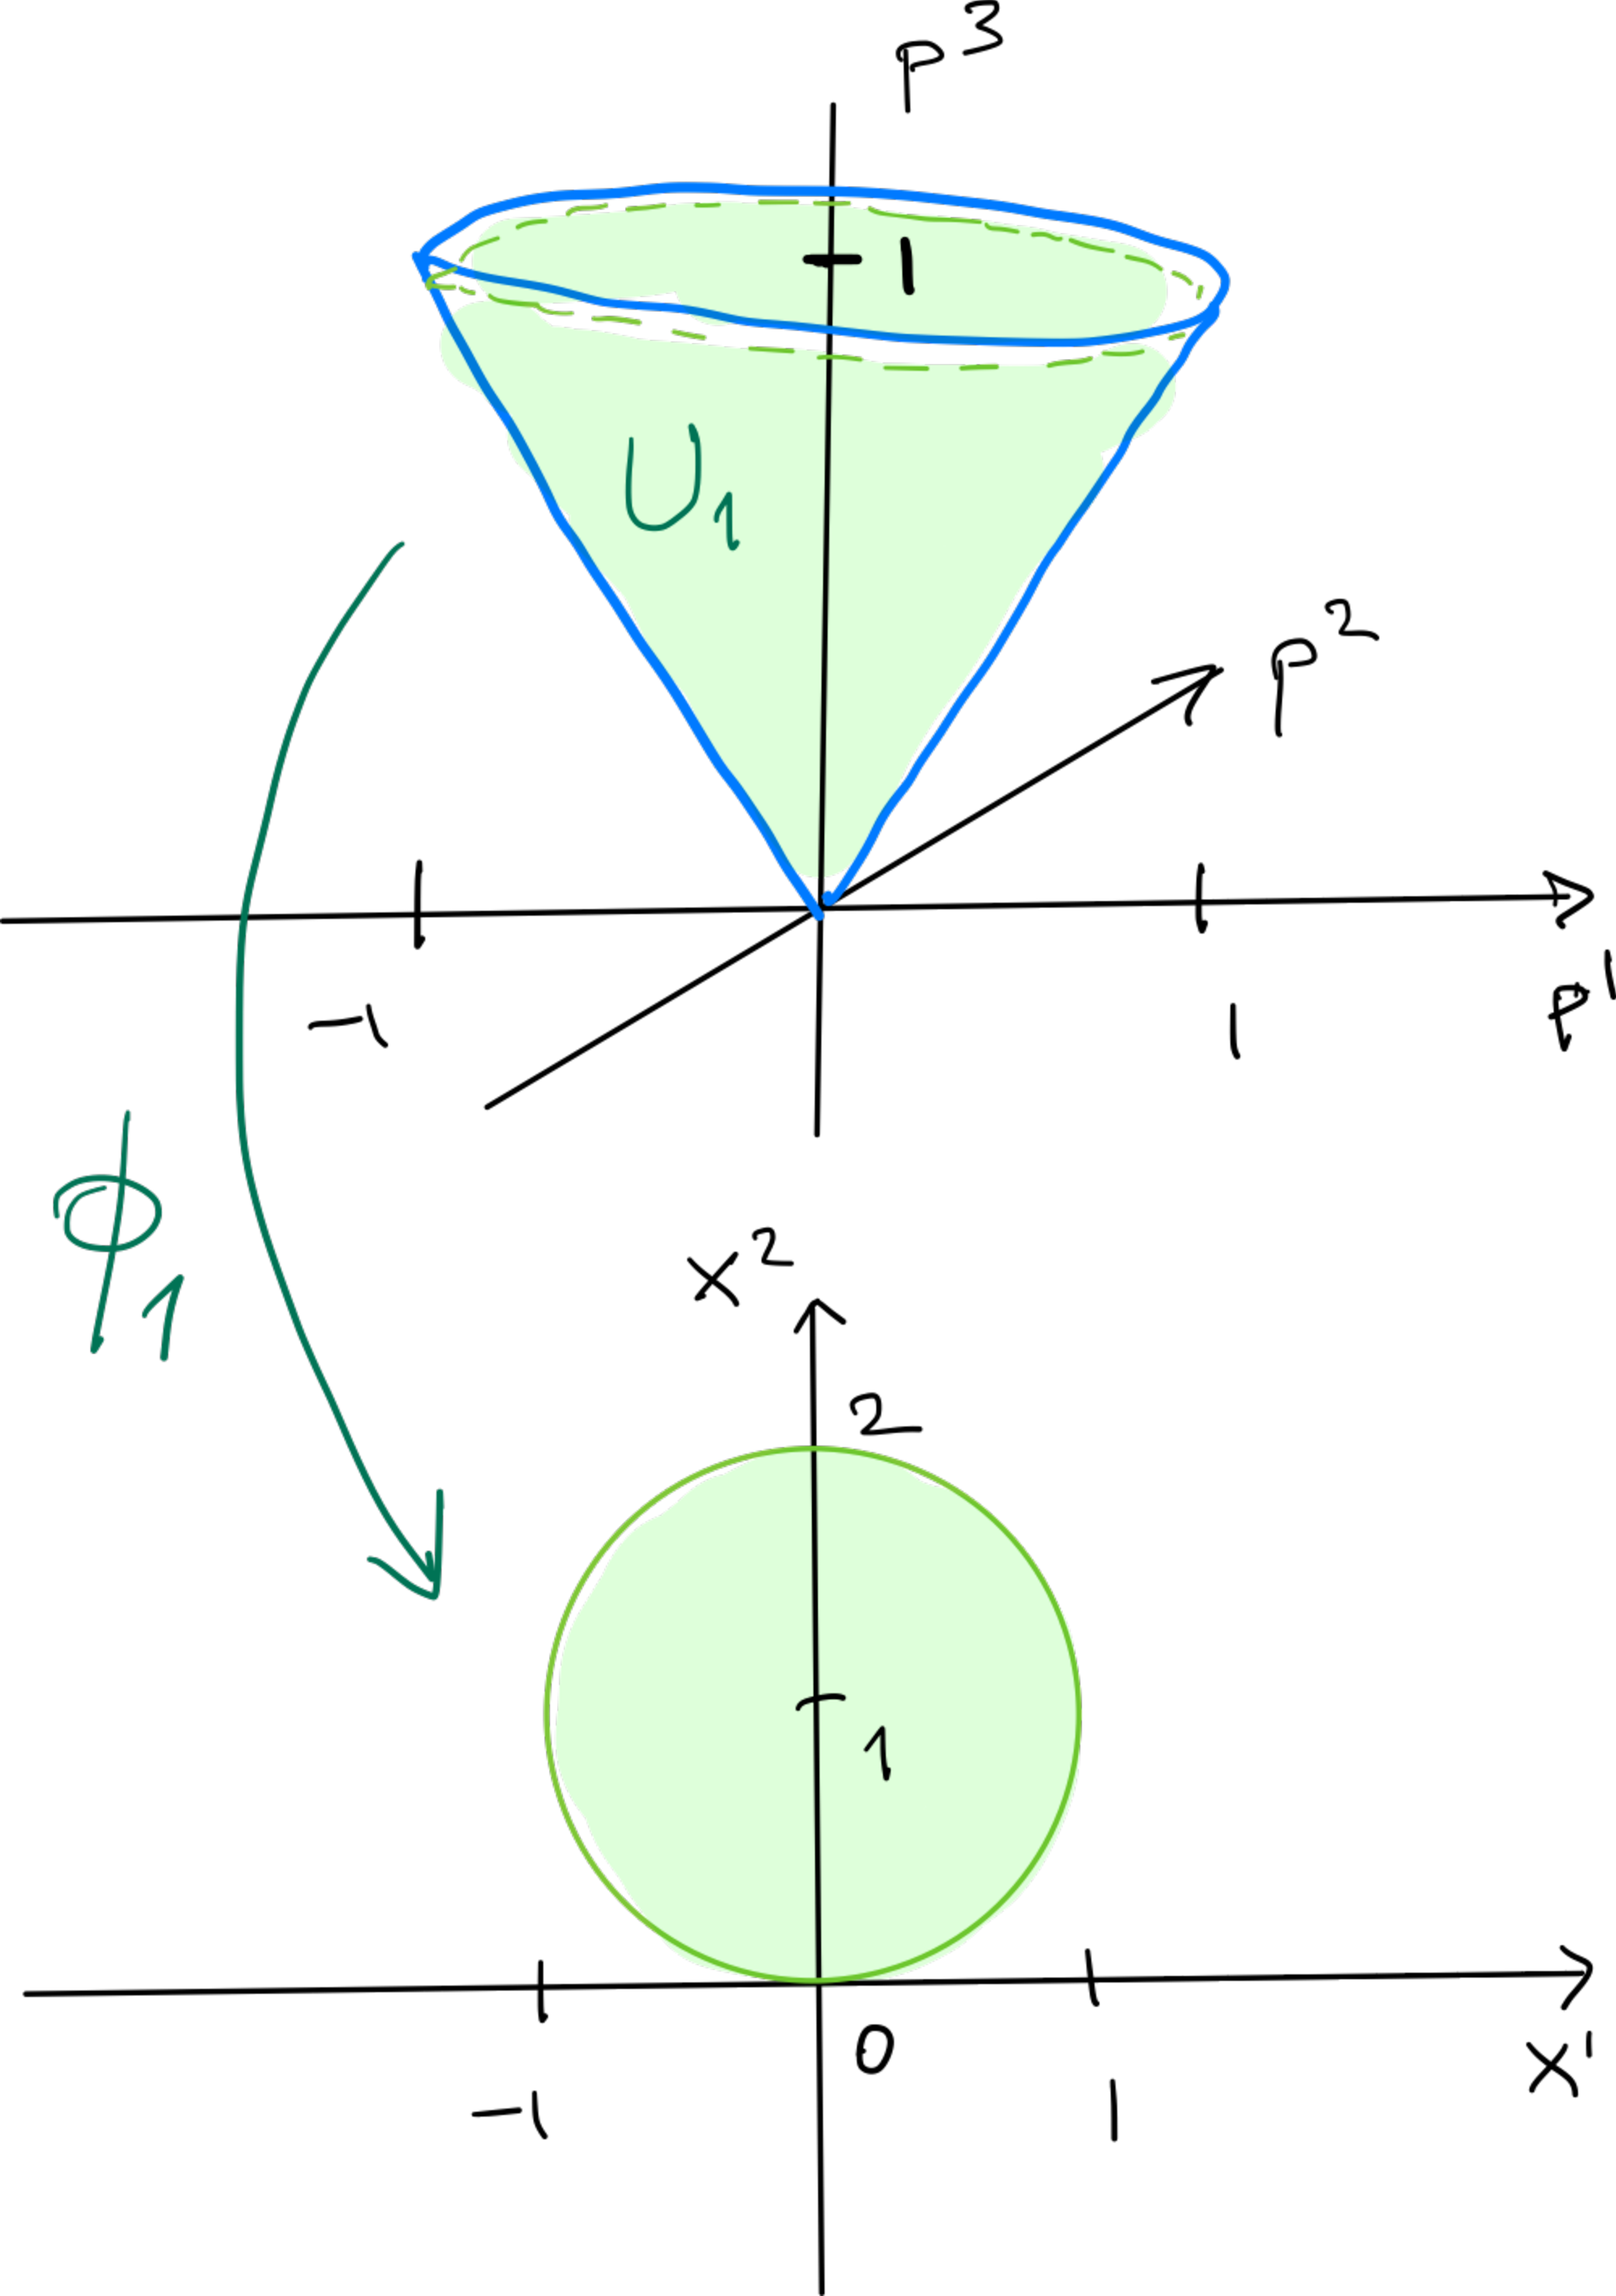
\includegraphics{1_5_9-cyl1}
  \end{marginfigure}
  We can describe the cone with the following atlas $\cA = \{(U_i,\varphi_i)\mid i=1,2,3\}$:
  \begin{itemize}
    \item $U_1 := \{p\in\cC\mid p^3 < 1\}$ with $x = (x^1, x^2) = \varphi_1(p) = (p^1,p^2+1)$, thus
      \begin{equation}
        \varphi_1^{-1}(x) = \left(x^1, x^2-1, \sqrt{(x^1)^2 + (x^2-1)^2}\right).
      \end{equation}
    \item $U_2 = \{p\in\cC\mid 1/2 < p^3 \leq 1, \; (p^1, p^2) \neq (0, p^3)\}$ with $\varphi_2$ defined as follows. Let
      \begin{equation}
        q = \psi(p) = \left(\frac{p^1}{p^3}, \frac{p^2}{p^3}, p^3\right)
        \quad\mbox{and}\quad
        \sigma(q) = \left(\frac{2q^1}{1-q^2}, 1-q^3\right),
      \end{equation}
      then $x = \varphi_2(p) = (\sigma\circ\psi)(p)$ and $\varphi_2(U_2) = \R\times[0,1/2) \subset\cH^2$.
    \item $U_3 = \{p\in\cC\mid 1/2 < p^3 \leq 1, \; (p^1, p^2) \neq (0, -p^3) \}$ and $\varphi_3$ defined similarly as in the previous point.
  \end{itemize}
  \begin{marginfigure}
    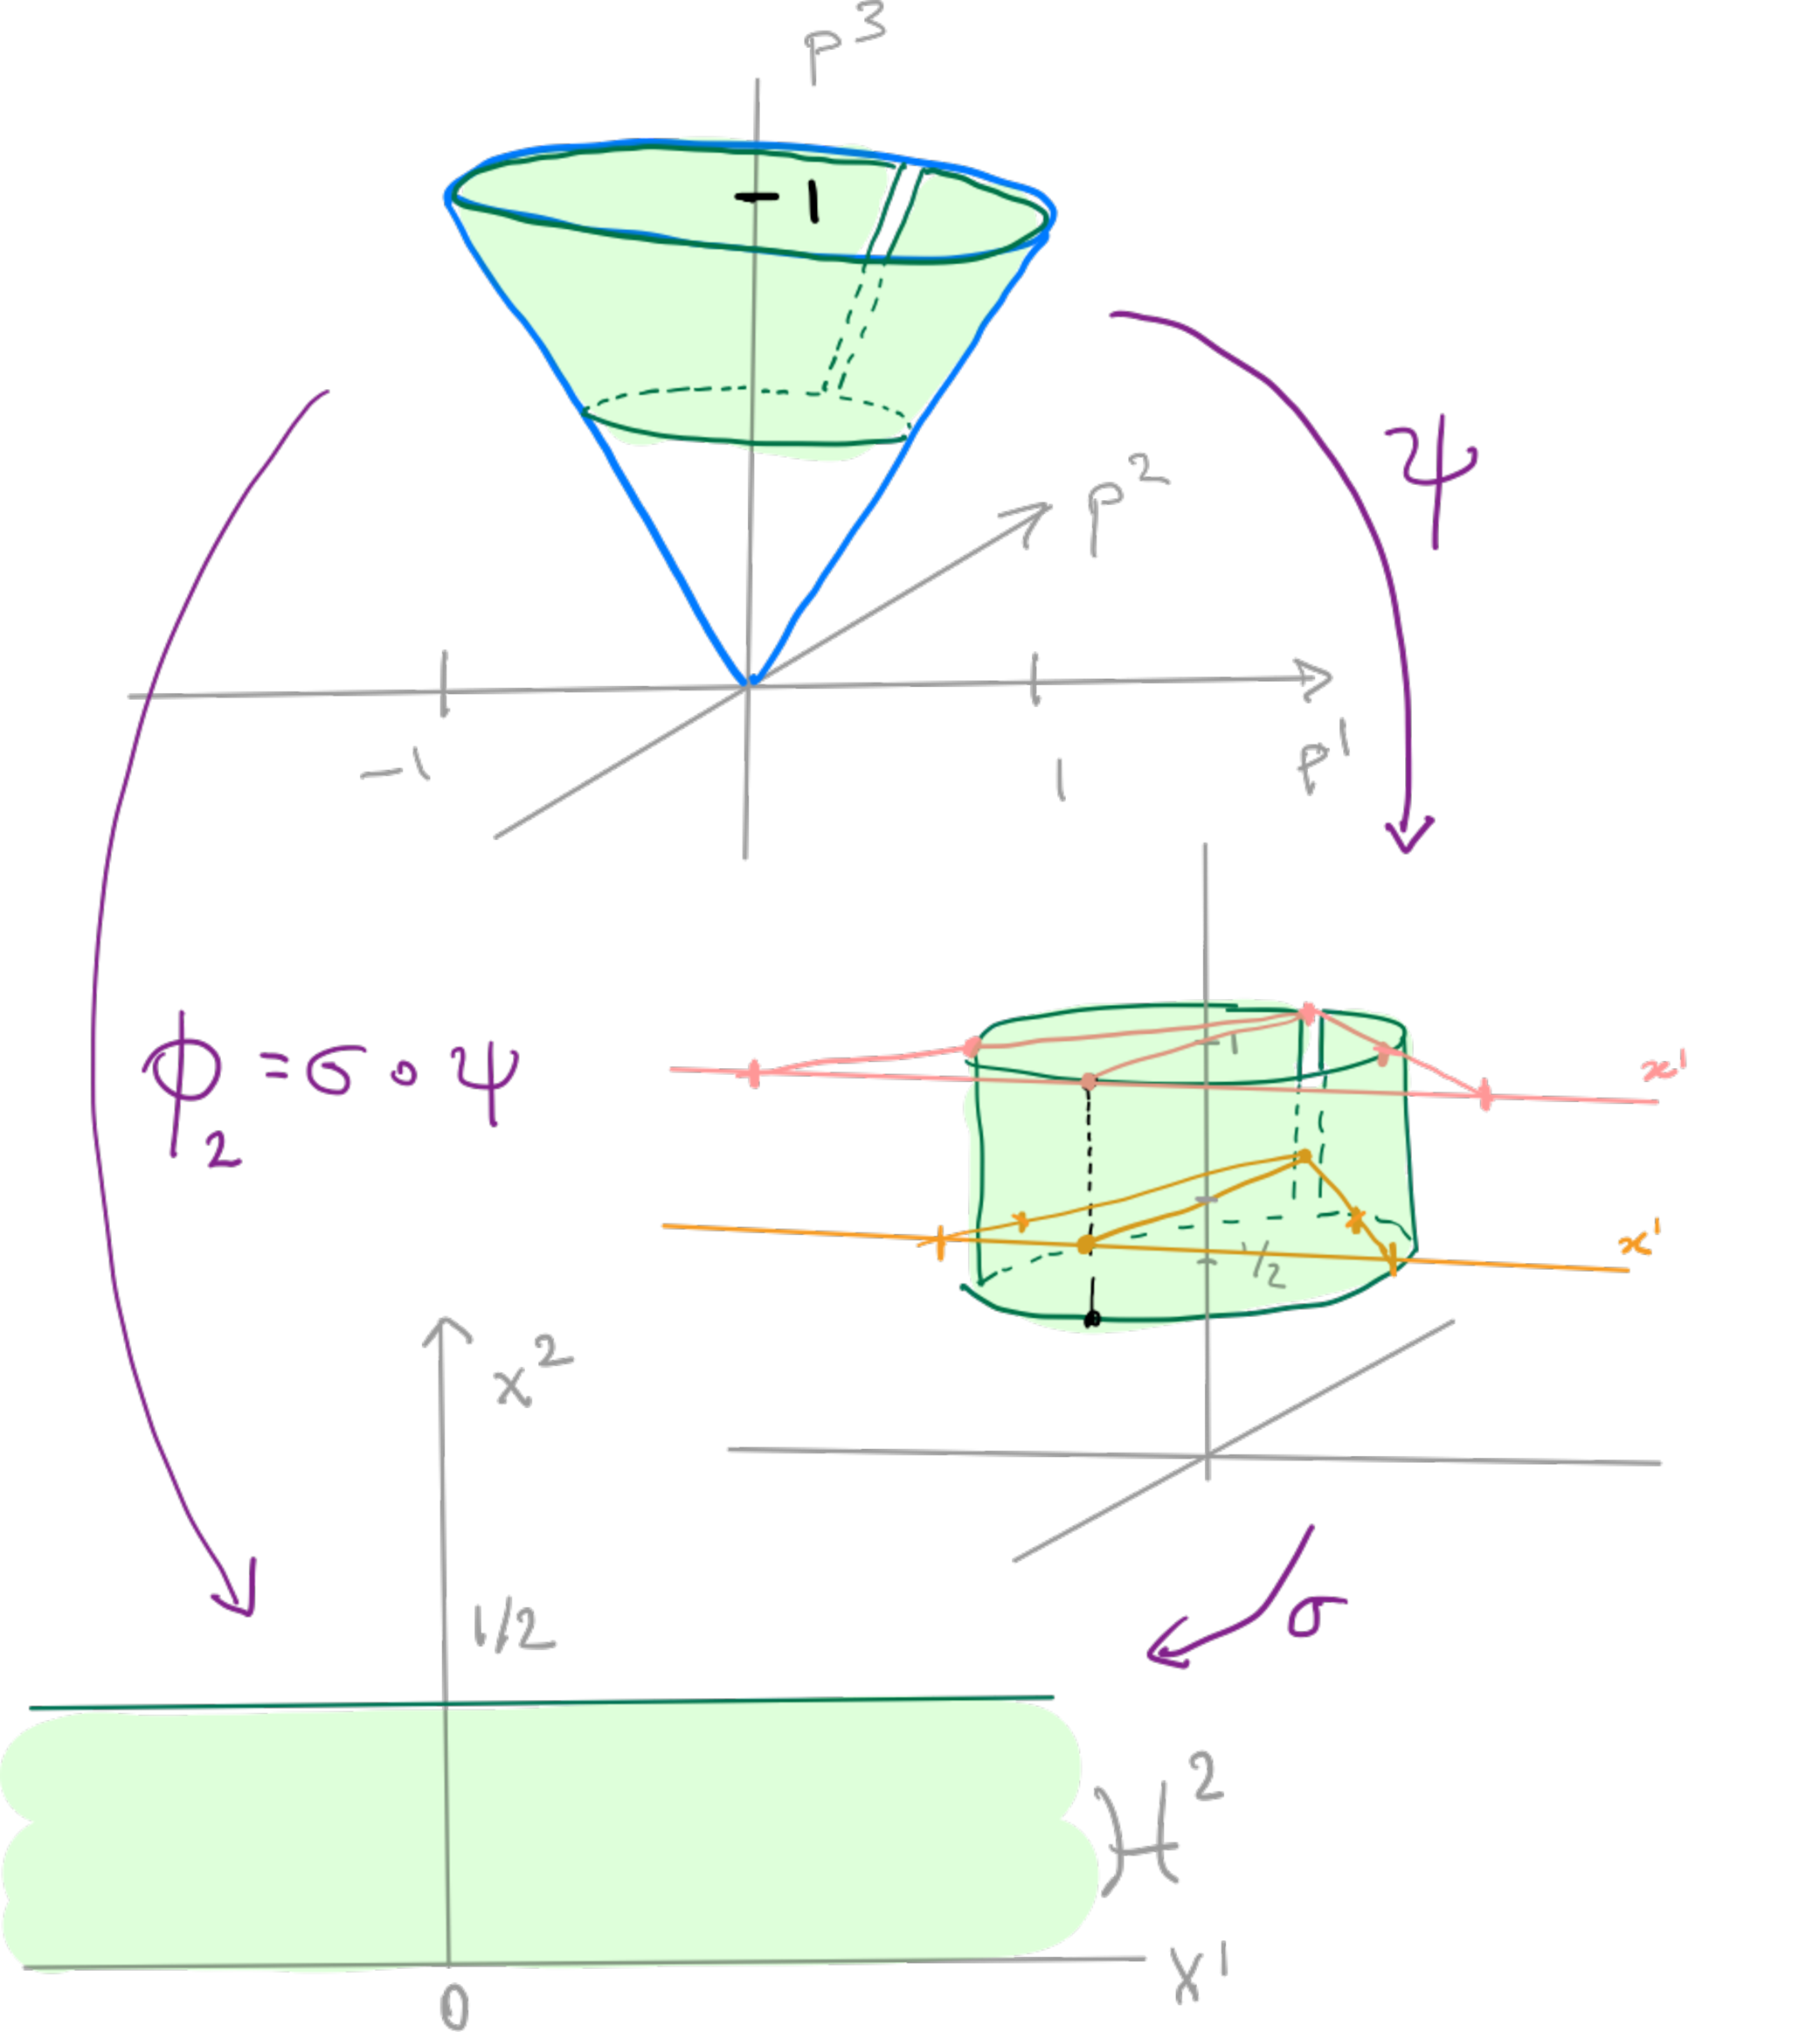
\includegraphics{1_5_9-cyl2}
    \caption{Compare $\varphi$ with the stereographic projections from Exercise~\ref{ex:stereo}. Do you notice any similarity?}
  \end{marginfigure}
  The boundary is given by $\partial\cC = \varphi_2^{-1}(\R\times\{0\}) \cup \varphi_3^{-1}(\R\times\{0\})$.
\end{example}

\begin{exercise}
  Explicitly define $\varphi_3$ from the previous example.
  Why is $\varphi_1$ not appearing in $\partial \cC$?
\end{exercise}

\begin{exercise}
  Let $M = D_1\subset \R^n$ be the $n$-dimensional closed unit ball from Example~\ref{ex:uball}.
  \begin{enumerate}
    \item Show that $M$ is a topological manifold with boundary in which each point of $\partial M = \bS^{n-1}$ is a boundary point and each point in $\mathring M = \{x\in\R^n\mid\|x\|<1\}$ is an interior point.
    \item Give a smooth structure to $M$ such that every smooth interior chart is a smooth chart for the standard smooth structure on $\mathring M$.\\
      \textit{\small Hint: consider the map $\pi\circ\sigma^{-1}:\R^n\to\R^n$ where $\sigma:\bS^n\to\R^n$ is the stereographic projection from Exercise~\ref{ex:stereo} and $\pi:\R^{n+1}\to\R^n$ is a projection that omits one of the first $n$ coordinates.}
  \end{enumerate}
\end{exercise}

\begin{tcolorbox}
  Differentiable manifolds without boundary (cf. Definition~\ref{def:diffmanifold}) can be thought as a special case of differentiable manifolds with boundary (cf. Definition~\ref{def:diffmanifoldwb}) where the boundary happens to be empty.
  Therefore, with the exception of the beginning of Chapter~\ref{ch:2}, we will no-longer distinguish the two concepts: from now on, a manifold may have or may not have a boundary.
\end{tcolorbox}


\chapter{Tangent bundle}\label{ch:2}
\section{Let the fun begin!}
\newthought{We are left to define derivatives} of functions between manifolds.
And, since we saw that euclidean spaces are manifolds, we better find a definition that coincides with the one you saw in your analysis courses.

\begin{marginfigure}[7em]
  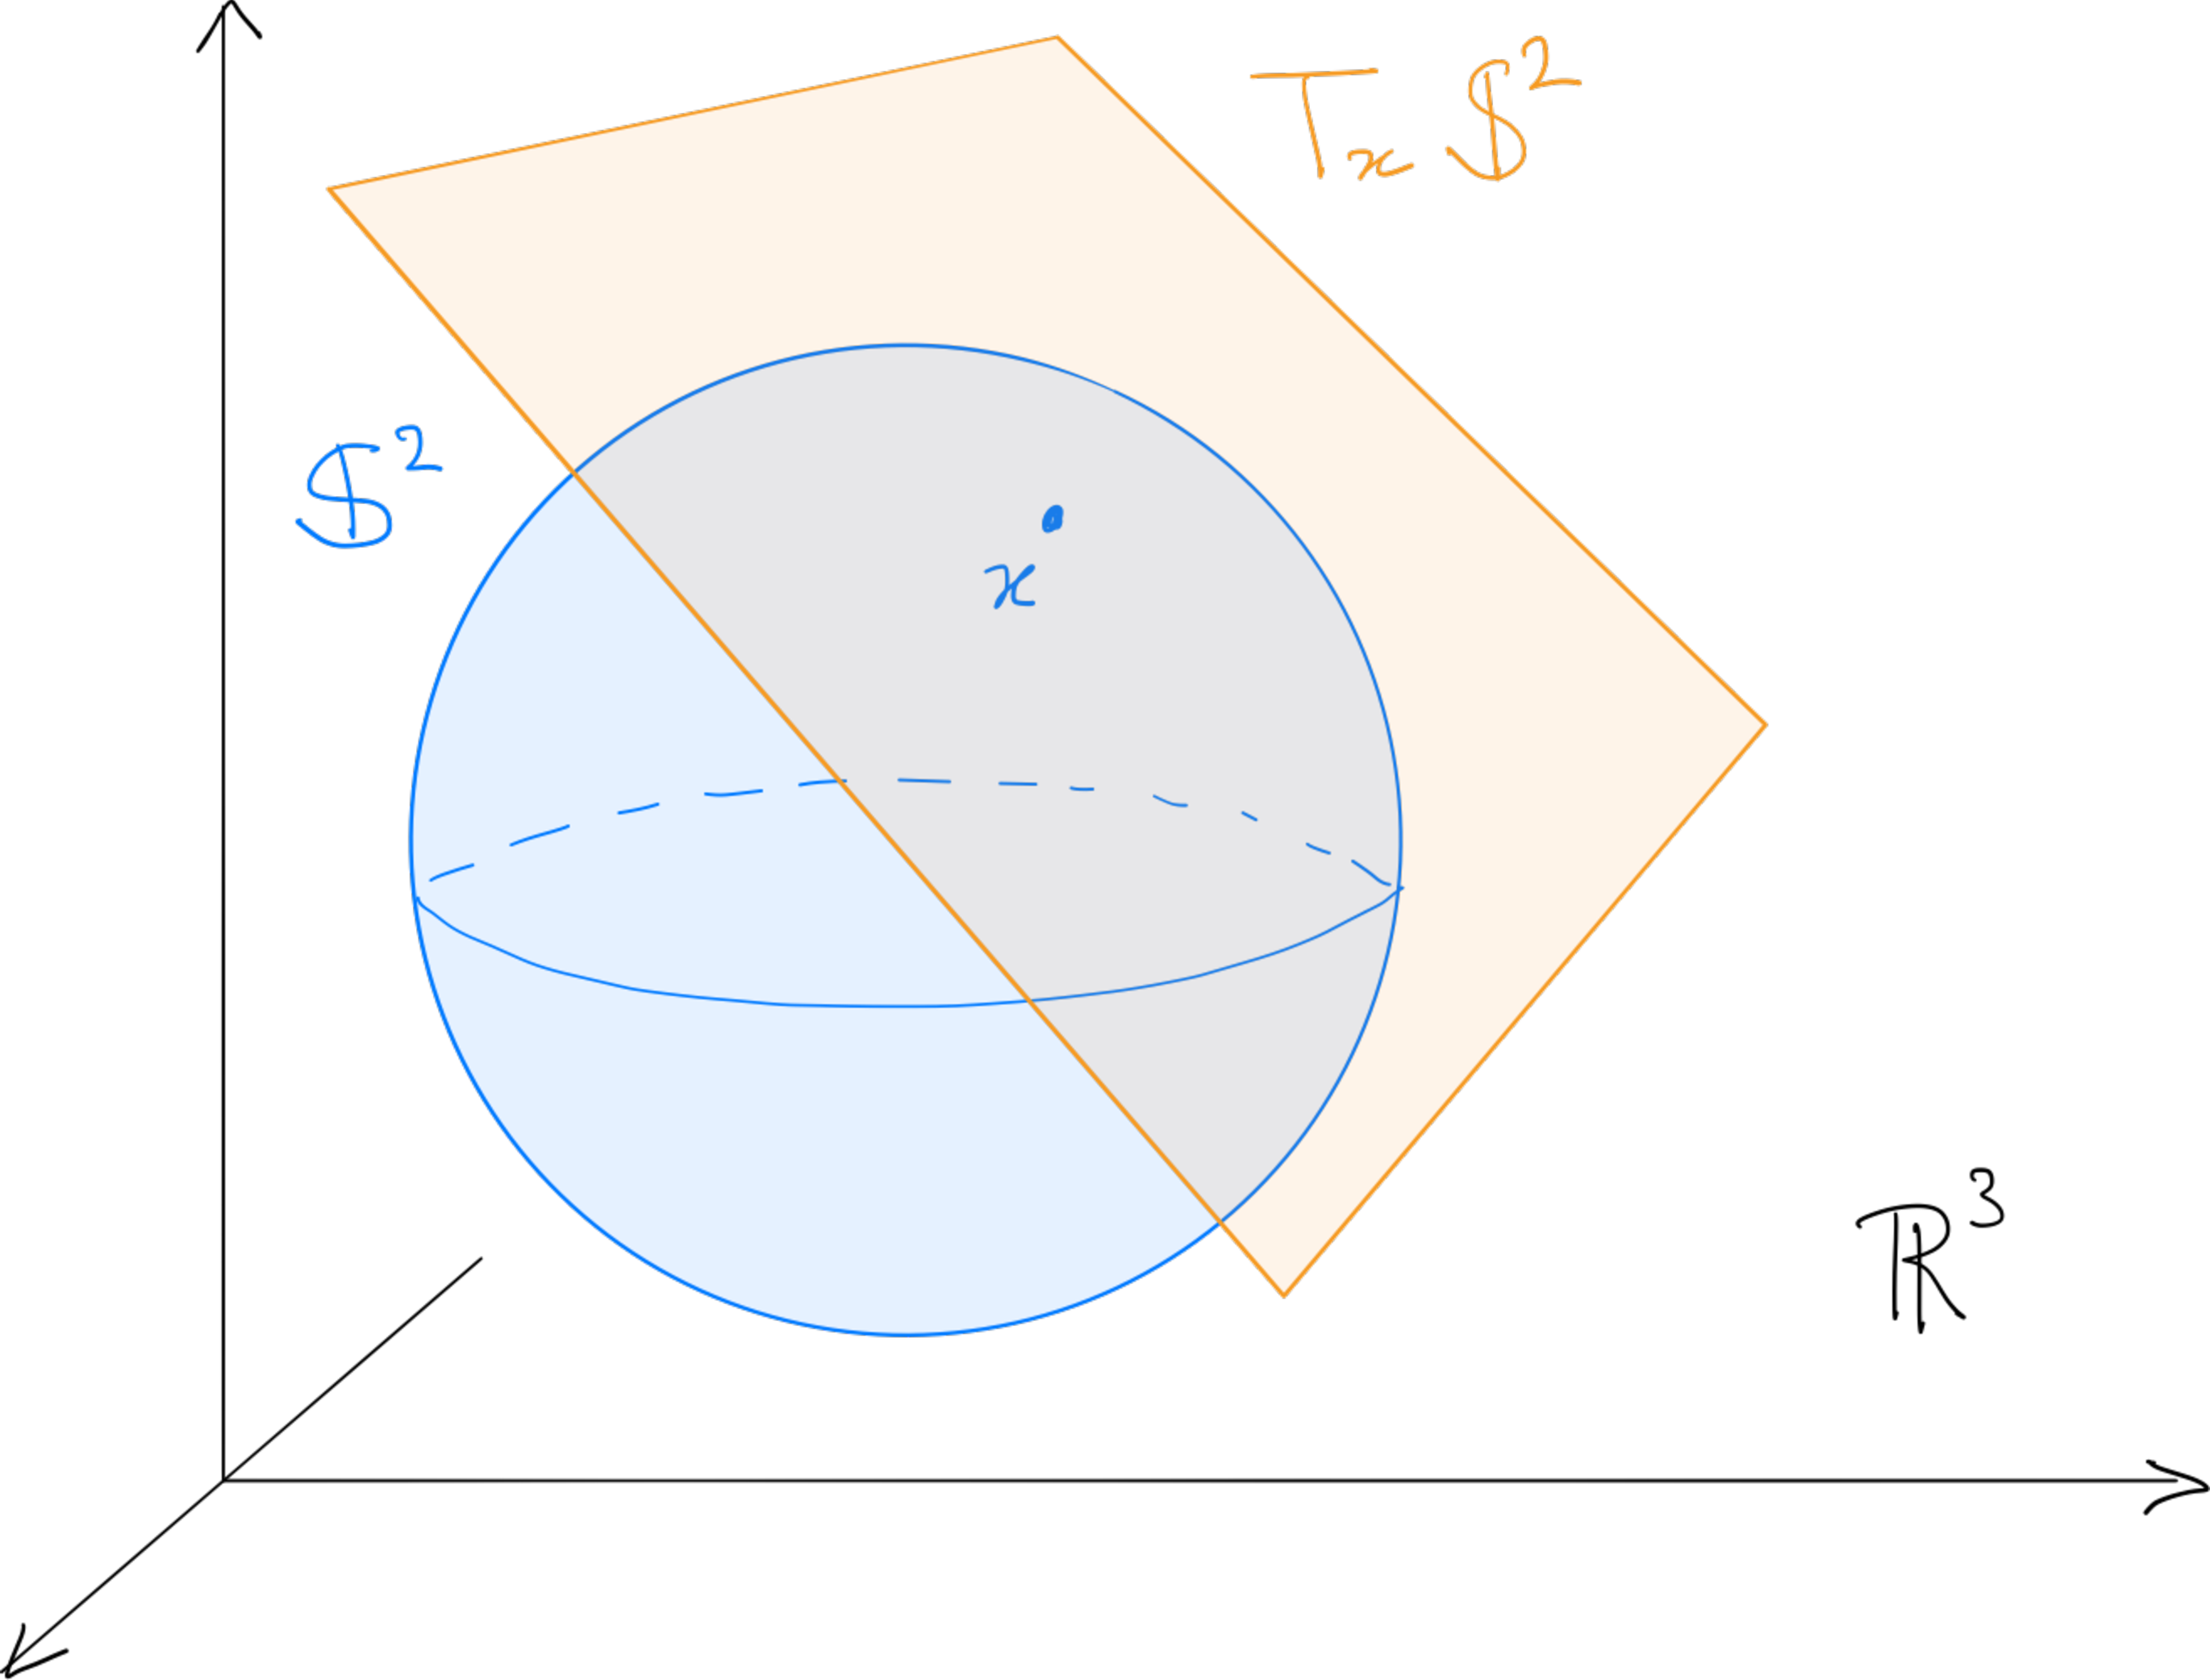
\includegraphics{2_1-embedded-sphere-tangent.pdf}
  \label{fig:tan-embedded-sphere}
  \caption{Tangent space to a point of a sphere $\bS^2$ embedded into the ambient space $\R^3$.}
\end{marginfigure}
In this chapter we will see how to associate to an $n$-dimensional smooth manifold $M$ an $n$-dimensional vector space, denoted by $T_x M$, to each point $x\in M$.
Such vector space is called \emph{tangent space to $M$ at $x$} and, for a manifold embedded into a euclidean ambient space, it will coincide with the intuitive understanding of a tangent hyperplane to the point on the manifold, see also Figure~\ref{fig:tan-embedded-sphere}.
As we will see, there are various different definition of tangent space but, in the end, they all turn out to be equivalent.

Due to a certain amount of freedom in terms of different ``perspectives'' leading to different but equivalent definitions, there is no unique way of introducing tangent spaces.
Just to give you an idea, all the following approaches lead to equivalent definitions (see also~\cite{book:lee}):
\begin{itemize}
  \item equivalence classes of curves through a point;
  \item transformation laws of the components of vectors with respect to different charts;
  \item generalization of linear approximation into the idea of an abstract derivation;
  \item derivations in the category of germs of functions;
\end{itemize}

It is also possible to ``flip'' the whole construction around, constructing differentials and cotangent spaces and using them to introduce the tangent spaces.
This is the approach taken by~\cite{lectures:hitchin} and it is at least worth of a look if you want to see a different perspective.

To avoid diverging from~\cite{book:tu} too much\footnote{Since it used to be the compulsory reading material in the previous years.}, we will stick to derivations on the space of germs, which emphasizes the locality of derivations to an extreme.
The equivalence between our approach and the one based on charts will be left as homework, while we will look into the equivalence with the speed of curves and with derivations together.

\section{Directional derivatives in euclidean spaces}\label{sec:dd}

Suppose that $f: U\subset\R^n\to\R^k$ is a smooth map defined on an open subset $U\subset \R^n$.
In multivariable calculus you have seen that if $x\in U$ and $v\in\R^n$, then the vector $Df(x) v$ can be interpreted as the directional derivative\footnote{Sometimes this is denoted $D_v f(x)$ instead.} of $f$:
\begin{equation}
  Df(x) v = \lim_{t\to0}\frac{f(x+tv) - f(x)}{t}.
\end{equation}
Then, the partial derivative is obtained as the particular case
\begin{equation}
  D_jf(x) := Df(x) e_j = \lim_{t\to0} \frac{f(x+te_j) - f(x)}{t}.
\end{equation}
Of course, we can also look at the derivative by using the standard euclidean coordinates $r^1, \ldots, r^n$, in that case we would be deriving $r^i \circ f : \R^n \to \R$.

\newthought{Let's take it slow}, and compare all these various derivatives next to each other.
For $f:U\subset\R^n\to\R^k$ and $x\in U$, we have
\begin{marginfigure}[3.5cm]
  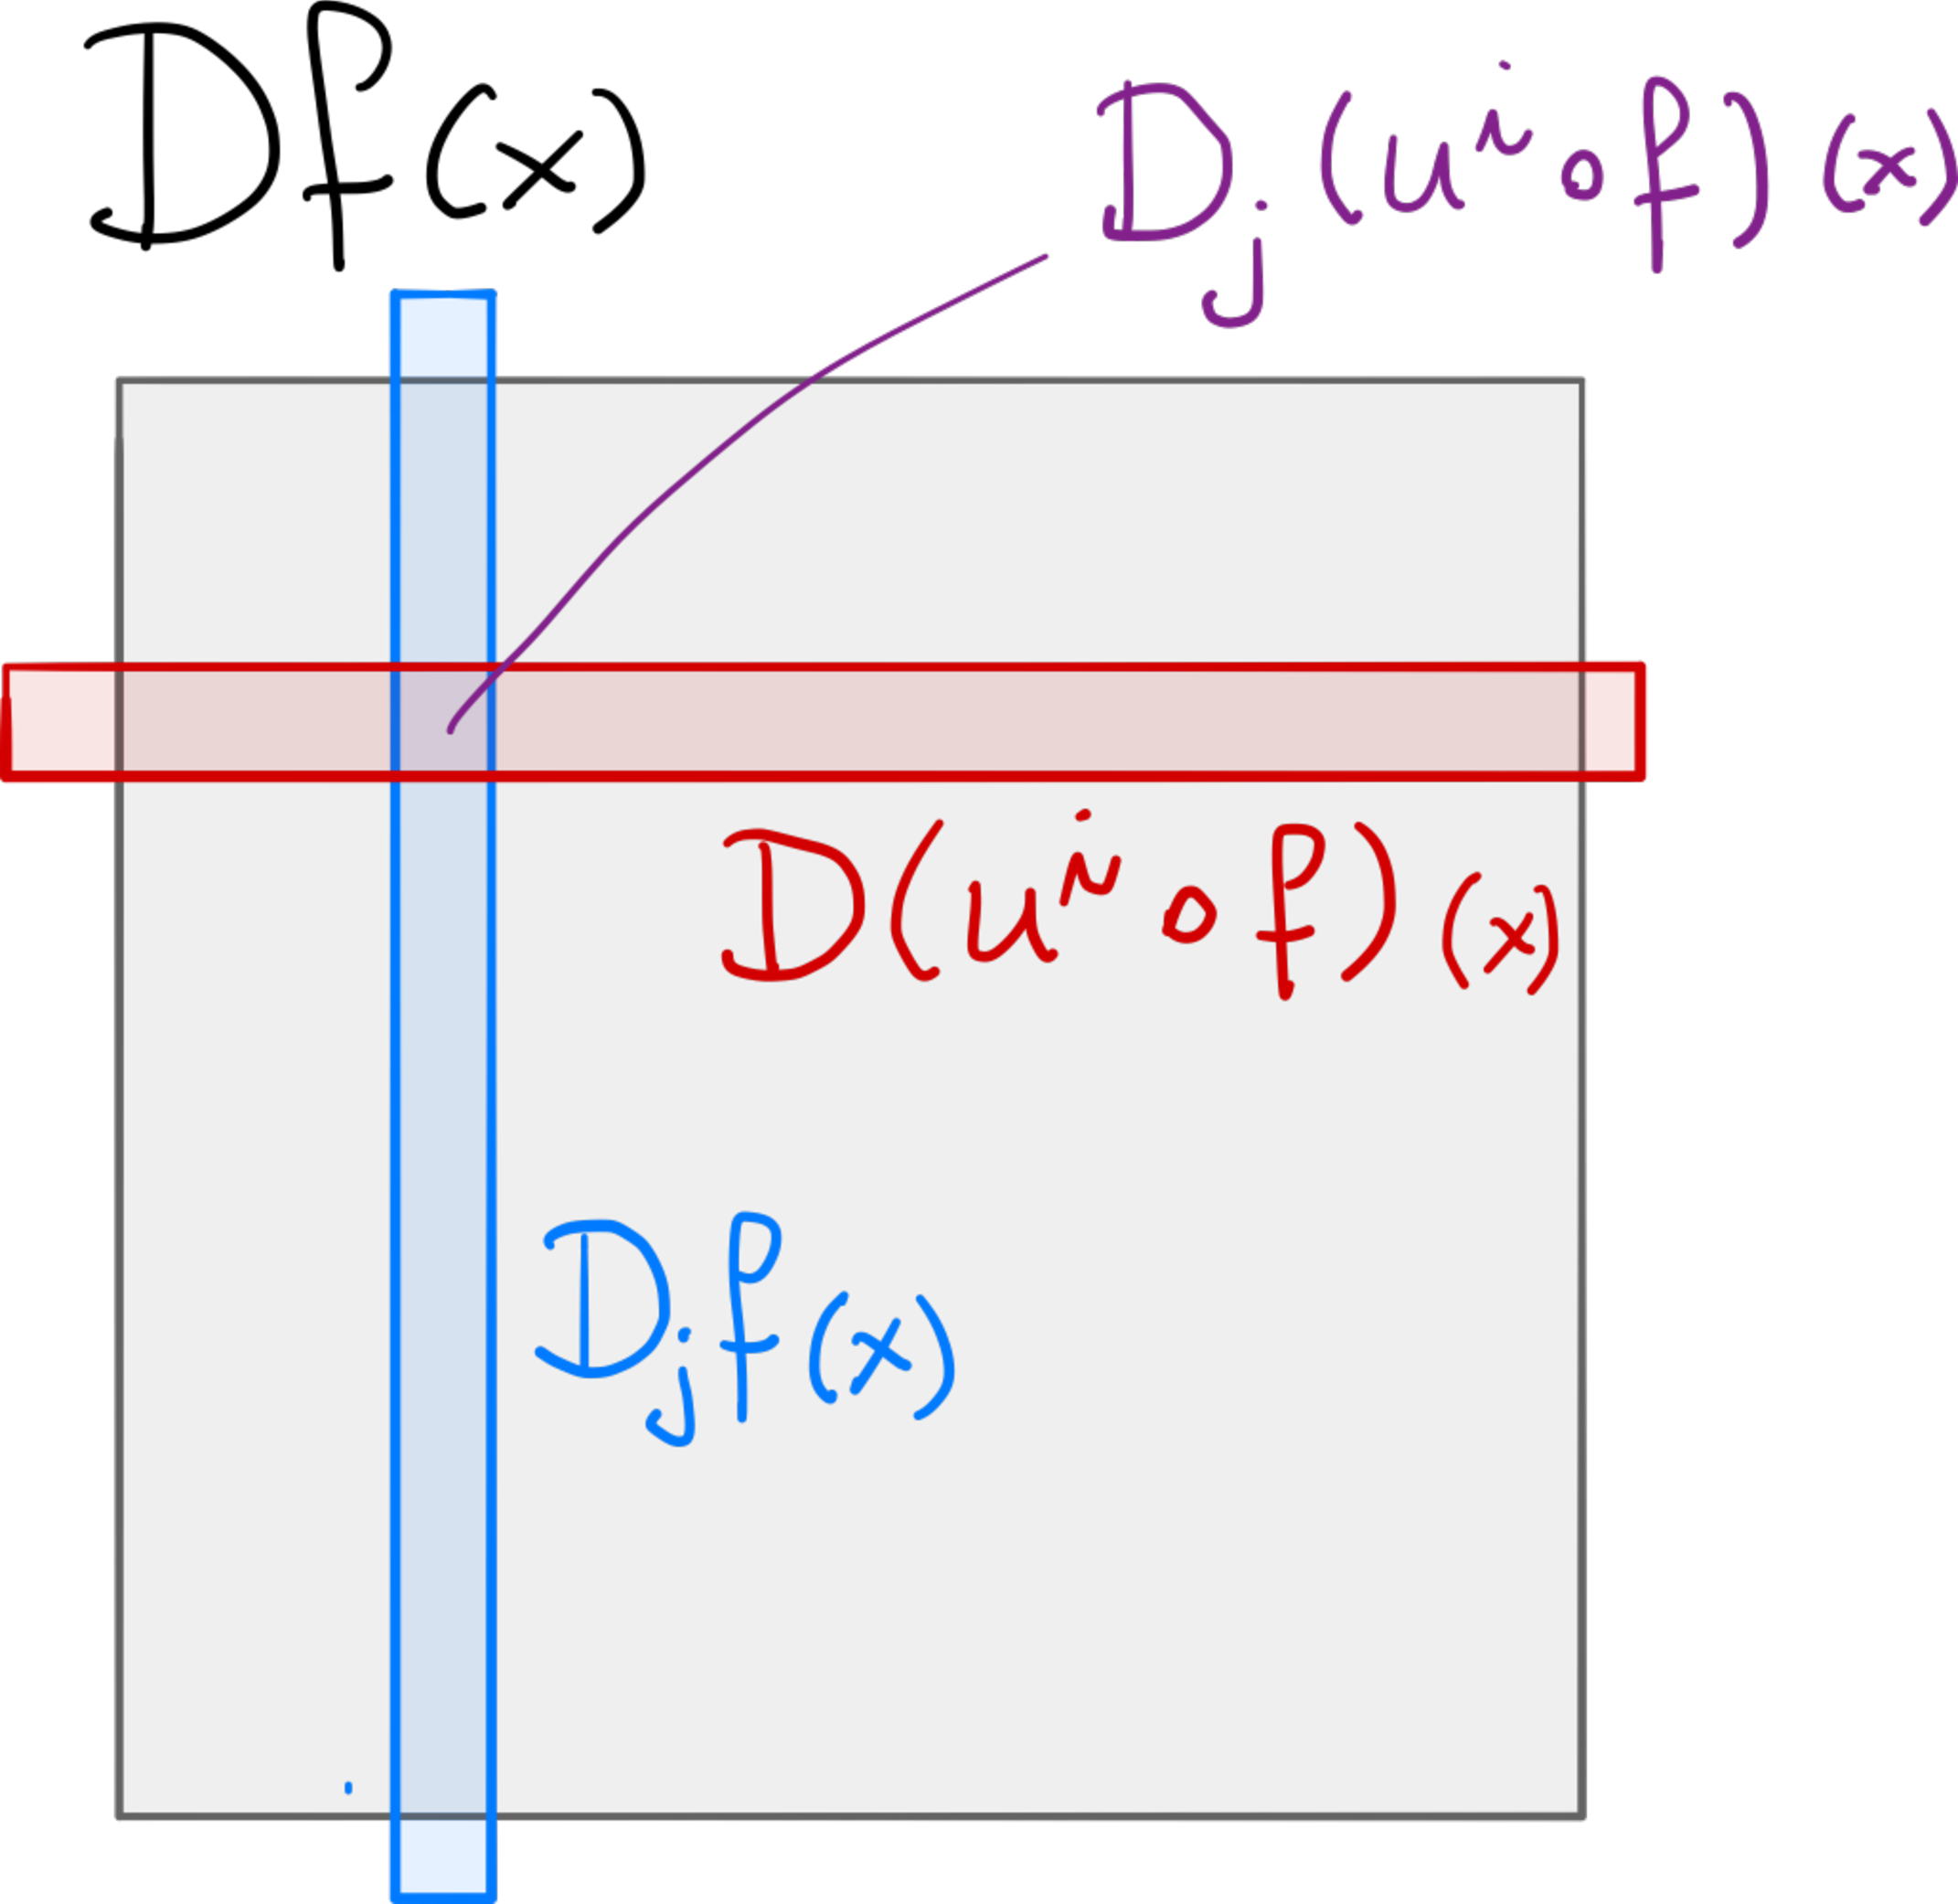
\includegraphics{2_3-ederivs.pdf}
\end{marginfigure}
\begin{itemize}
  \item $Df(x)$, the Jacobian matrix, which is a $k\times n$ matrix;
  \item $D_j f(x)$, the $j$th column of the matrix $Df(x)$, which is an element of $\R^k$;
  \item $D(r^i\circ f)(x)$, a linear function from $\R^n \to \R$, which one can think as the $i$th row of the matrix $Df(x)$;
  \item $D_j(r^i\circ f)(x) = \frac{\partial f^i}{\partial x^j}(x)$, a number in $\R$, which corresponds to the $(i,j)$th element $(Df(x))_j^i$ of the matrix $Df(x)$.
\end{itemize}

This notation using $D$ instead of spelling out the partial derivatives, comes with an important advantage.
Let's use it to rewrite the chain rule form Proposition~\ref{thm:chainrule}(\ref{thm:chainrule2}):
\begin{equation}
  D_j(r^i\circ g \circ f) (x) = \sum_{l=1}^k D_l(r^i\circ g)(f(x))\; D_j(r^l \circ f)(x),
\end{equation}
\marginnote[-4em]{Using Einstein notation, since $l$ is the only index that appears both in lower and upper position, $D_j(r^i\circ g \circ f) (x) = D_l(r^i\circ g)(f(x))\; D_j(r^l \circ f)(x)$.}
where $1\leq i\leq m, 1\leq j \leq n$.
As you can see, we do not need to explicitly spell out the derivatives in local coordinates on $\R^n$ or $\R^k$ in this new formula.
This will prove extremely convenient for the development of the theory.

\section{Germs and derivations}

\newthought{To reach our goal of defining derivations on manifolds}, a direct extension of partial derivatives is not enough: we will need to introduce some more levels of abstraction.

\begin{definition}
  Let $M$ be a smooth manifold.
  For some point $p\in M$, let $U,V\subset M$ be two neighbourhoods of $p$.
  We say that two functions $f\in C^\infty(U)$ and $g\in C^\infty(V)$ have the same \emph{germ} at $p$ if there exists a neighbourhood $W\subset U\cap V$ of $p$ such that $f|_W \equiv g|_W$.
\end{definition}

Germs define an equivalence relation on the set of smooth functions defined on a neighbourhood of a point $p$: $(U, f) \sim_p (V, g)$ if they have the same germ at $p$. Then, a germ $[f]_p$, where $(U, f)$ is one representative for $[f]_p$, is an equivalence class in the quotient space 
\begin{equation}
  C_p^\infty(M) := C^\infty(M)/\!\sim_p.
\end{equation} 

\begin{exercise}
  Show that $\sim_p$ defined above is an equivalence relation in $C^\infty(M)$.
\end{exercise}

For $c\in\R$ and $[f]_p, [g]_p$ germs with representatives $(U, f), (V, g)$, we have
\begin{itemize}
  \item $[f]_p + [g]_p$ is the germ with representative $(U\cap V, f+g)$;
  \item $[f]_p [g]_p$ is the germ with representative $(U\cap V, f g)$;
  \item $c[f]_p$ is the germ with representative $(U, cf)$.
\end{itemize}
Therefore, $C_p^\infty(M)$ is also an algebra over $\R$.

\begin{exercise}
  Check that the operations above are well--defined.
\end{exercise}

Germs are the apotheosis of locality: a germ at $p$ has a well--defined value at $p$ and nowhere else.
This results in a map,
\begin{equation}
  \eval_p: C_p^\infty(M) \to \R, \quad
  \eval_p([f]_p) := f(p),
\end{equation}
where $(V,f)$ is any representative of $[f]_p$.
\begin{exercise}
  Check that the $\eval_p$ map is well--defined.
\end{exercise}

We can now go back to our discussion of euclidean derivations to motivate our definition of tangent vectors.

\begin{example}\label{ex:euclideanD}
  Let $U\subset\R^n$ open\footnote{In what follows, we will think at $U$ both as an open subset of $\R^n$ and a smooth manifold depending on what is most convenient for us.} and $f\in C^\infty(U)$.
  For $x\in U$ and $v\in\R^n$ we have seen that $Df(x)$ can be interpreted as a matrix that consumes the vector $v$ to produce a number $D(f)v$.
  In such interpretation $f$ is fixed and only $x$ and $v$ vary, however there is no reason for this restriction.

  Indeed, an alternative interpretation lets also $f$ vary and consider the action of differentiation as a map
  \begin{equation}
    U \times \R^n \times C^\infty(U) \to \R,\quad
    (x,v,f) \mapsto Df(x) v.
  \end{equation}
  And since we are flipping around all the ideas, let us consider $x$ and $v$ fixed and instead only let $f$ vary:
  \begin{equation}\label{eq:mapxvtoD}
    (x,v):C^\infty(U) \to\R, \quad (x,v)(f) := Df(x)v.
  \end{equation}
  By the definition~\eqref{eq:diff} of the euclidean differential, we know that it is a local property: the value $Df(x)$ only depends on the germ of $f$ at $x$.
  Thus we can rephrase~\eqref{eq:mapxvtoD} by saying that $v$ defines a \emph{linear} map
  \begin{equation}
    v : C_x^\infty(U) \to \R, \quad
    v([f]_x) := Df(x) v.
  \end{equation}
  In fact, this is not just a linear map, it also satisfies a \emph{derivation} property, in the sense that
  \begin{equation}
    v([f]_x [g]_x) =
      \eval_x([f]_x)v([g]_x)
      + \eval_x([g]_x)v([f]_x).
  \end{equation}
  Which, rewritten in a more familiar form, is just a way to rewrite the \emph{Leibniz rule}:
  \begin{equation}
    D(fg)(x) v = f(x)Dg(x)v + g(x) Df(x)v.
  \end{equation}

  Note that we have now two different interpretations for $v$: it is both a vector in $\R^n$ and a linear map $C_x^\infty(U) \to \R$ satisfying the derivation property.
\end{example}

Motivated by Example~\ref{ex:euclideanD}, we will define a tangent vector as a derivation on the space of germs.

\begin{definition}
  Let $M$ a smooth manifold of dimension $n$ and let $p\in M$.
  A \emph{tangent vector at $p$} is a linear map
  \marginnote{Keep always in mind that the value $v([f]_p)$ only depends on the value of $f$ around the point $p$.}
  \begin{equation}\label{def:tangentvector}
    v: C_p^\infty(M)\to\R
  \end{equation}
  which is also a derivation, i.e.
  \begin{equation}
    v([f]_p [g]_p) =
      \eval_p([f]_p)v([g]_p)
      + \eval_p([g]_p)v([f]_p).
  \end{equation}

  Since a tangent vector is a linear map from the vector space $C_p^\infty(M)$ to $\R$, the set of all tangent vectors at a point $p$ is itself a vector space\footnote{Exercise: why is this true?} which we denote by $T_p M$.
\end{definition}

Let's check that these vectors, at least satisfy the most elementary properties of derivations: one would expect the derivative of constant functions to be zero, is that the case?

\begin{lemma}\label{lem:f'0is0forconst}
  Let $M$ be a smooth manifold, let $U\subset M$ be an open set containing $p$ and let $v\in T_p M$.
  Denote by $[c]_p$ the germ of a constant function $(U, p \mapsto c)$.
  Then $v([c]_p) = 0$.
\end{lemma}
\begin{proof}
  Since $[c]_p = c [1]_p$, by linearity we have $v([c]_p) = c v([1]_p)$.
  Thus, it will be enough to show that $v([1]_p) = 0$.
  Since $v$ is a derivation, using the algebra properties of the space of germs we get
  \marginnote{Keep this simple trick in mind, it will be useful in the future.}
  \begin{equation}
    v([1]_p) = v([1]_p [1]_p) = 2 \eval_p([1]_p)v([1]_p) = 2 v([1]_p).
  \end{equation}
  Thus, $v([1]_p) = 0$, concluding the proof.
\end{proof}

As you can see, working with equivalence classes is doable but unnecessarily cumbersome.
As we did with atlases, we would like to get it over with.

\begin{definition}
  Let $M$ be a smooth manifold and $p\in M$.
  Let $W\subseteq M$ be any neighbourhoods of $p$.
  \marginnote{We are still talking about derivations of functsion at specific points, not to be confused with the derivations of the algebra $C^\infty(W)$ which we will introdce later and will be maps of the kind $C^\infty(W)\to C^\infty(W)$.}
  A map $w:C^\infty(W)\to\R$ is called a \emph{derivation of $C^\infty(W)$ at $p$} if it is linear over $\R$ and satisfies Leibniz rule
  \begin{equation}
    w(fg) = f(p)w(g) + g(p)w(f).
  \end{equation}
\end{definition}

If $v\in T_p M$, then we already saw that $v$ naturally defines a derivation $w$ of $C^\infty(W)$ for any open neighbourhood $W$ of $p$.
In this case
\begin{equation}\label{eq:derivfromtg}
  w(f) := v([f]_p).
\end{equation}
Showing that the opposite is also true will require a bit of work.

\begin{proposition}
  Let $M$ be a smooth manifold, $p\in M$ and $W$ any neighbourhood of $p$.
  Then there is a linear isomorphism between $T_p M$ and the space of derivations of $C^\infty(W)$ at $p$.
\end{proposition}
\begin{proof}
  To prove the theorem we need to invert~\eqref{eq:derivfromtg} and define a tangent vector in terms of of a derivation of $C^\infty(W)$ at $p$.
  We will proceed in three steps

  \newthought{Step I}. Let $w:C^\infty(W) \to\R$ be a derivation at $p$ and suppose that $f\in C^\infty(W)$ is identically zero on a neighbourhood $W_0\subset W$ of $p$. We are going to show that $w(f)=0$.

  By Proposition~\ref{prop:cutoff}, we can find a cutoff function $\rho:M\to\R$ such that $\rho(p)=1$ inside $W_0$ and $\supp(\rho) \subset W_0$. Consider now $g = \rho f : W \to \R$. Then $g$ is identically zero in the whole $W$, and thus\footnote{Follows by linearity, exactly as in Lemma~\ref{lem:f'0is0forconst}} $w(g) = 0$. Using Leibniz rule, the fact that $\rho(p)=1$ and $f(p) = 0$, we get
  \begin{equation}
    0 = w(g) = w(\rho f) = \rho(p) w(f) + f(p)w(\rho) = w(f).
  \end{equation}

  \newthought{Step II}.
  Let $[f]_p\in C_p^\infty(M)$.
  We want to show that it is always possible to find a representative for $[f]_p$ with domain $W$, that is, there exists $g\in C^\infty(W)\to\R$ such that $[g]_p = [f]_p$.
  Let $(V, f)$ be any representative of $[f]_p$.
  Since germs are local, if necessary, we can shrink $V$ so that $V\subset W$.
  Here comes the tricky bit: we need to extend $f$ to a function $g$ defined on $W$ which coincides with $f$ in some neighbourhood of $p$!
  To this end, choose\footnote{We can do this because topological manifolds are locally compact Hausdorff spaces, which implies that every point has a neighbourhood with compact closure. You can take it for granted or have a look at e.g.~\cite[Lemma 4.65]{book:lee:topology} or~\cite{book:munkres:topology}.} a smaller neighbourhood $U$ of $p$ such that $\overline{U}\subset V\subset W$.
  Again, Proposition~\ref{prop:cutoff} comes to the rescue. Apply it with $K=\overline{U}$ and ``$U$'' equal to $V$, and consider
  \begin{equation}
    g:W\to\R, \quad
    g(q) := \begin{cases}
      \rho(q)f(q), & q\in V,\\
      0, & q \in W\setminus V.
    \end{cases}
  \end{equation}
  Since $g|_U = f$, we have $[g]_p = [f]_p$, proving the claim.

  \newthought{Step III}. We can now complete the proof.
  Let $w:C^\infty(W) \to\R$ be a derivation at $p$.
  A tangent vector is a linear map $v:C_p^\infty(M)\to\R$, see~\eqref{def:tangentvector}, and a derivation.
  We would like to define one in terms of $w$.
  Given any $[f]_p\in C_p^\infty(W)$, the previous step guarantees that there exists a representative $(W,f)$ for it, so we can define
  \begin{equation}
    v([f]_p) := w(f), \quad\mbox{where $(W,f)$ is any representative of $[f]_p$}.
  \end{equation}
  Such $v$ is a derivation by construction, so if it is well-defined, we are done.
  To this end, assume that there exists a different representative $(W, g)$ for $[f]_p$.
  Then, by definition, there exists a neighbourhood $V\subset W$ of $p$ such that $f|_p = g|_p$.
  By linearity, $w(f) - w(g) = w(f-g)$ and by the first step in the proof, $w(f-g) = 0$.
  
  The assignment $w\mapsto v$ inverts~\eqref{eq:derivfromtg}, completing the proof.
\end{proof}

This seemingly innocent proposition, has some very important consequences.

First of all, from now on we are free to interpret tangent vectors in $T_p M$ as derivations of $C^\infty(W)$ at $p$ for \emph{any}\footnote{In particular, it is often convenient to have $W$ coincide with the domain of a chart or with the whole manifold $M$.} open $W$ containing $p$.
This enables us to give our first example of tangent vector.

\begin{example}\label{ex:partialderivative}
  Let $M$ be a smooth manifold of dimension $n$ and $\varphi: U \to V\subset\R^n$ a chart on $U\subset M$.
  As already mentioned, we write $x^i = r^i \circ \varphi$ for the local coordinates\footnote{See Notation~\ref{ntn:coords}.} of $\varphi$.
  For any $p\in U$, we can define a derivation of $C^\infty(U)$ at $p$ as
  \begin{equation}
    \frac{\partial}{\partial x^i}\Big|_p : C^\infty(U) \to \R, \quad
    \frac{\partial}{\partial x^i}\Big|_p (f) := \frac{\partial f}{\partial x^i}(p) := D_i(f\circ\varphi^{-1})(\varphi(p)).
  \end{equation}
  From now on, it will get more and more convenient to draw commutative diagrams to see ``how things are moving around'':
  \begin{equation}
    \begin{tikzcd}[column sep = huge, row sep = huge]
      M\supset U \arrow[r, "\varphi" description] \arrow[d, "f" description] & V \subset\R^n \arrow [dl, "f\circ\varphi^{-1}" description]\\
      \R &
    \end{tikzcd}
  \end{equation}
  We will soon see that $\left\{\frac{\partial}{\partial x^i}\Big|_p \mid 1\leq i\leq n\right\}$ forms a basis for $T_p M$.
\end{example}

Secondly, it provides us some very useful corollaries.

\begin{corollary}\label{cor:tgsubspace}
  Let $M$ be a smooth manifold and let $W\subset M$ be a non-empty open set considered as a smooth manifold.
  Then, for any $p\in W$ there is a canonical identification $T_pW = T_p M$.
\end{corollary}

\begin{corollary}\label{cor:derzero}
  Let $M$ be a smooth manifold and $p\in M$.
  Let $W\subseteq M$ be an open neighbourhood of $p$.
  If $f\in C^\infty(W)$ is constant in a neighbourhood of $p$, then $v(f) = 0$ for all $v\in T_p M$.
\end{corollary}

With these new tools at hand, we are ready to state and prove an important result on the size of the tangent spaces.
As it turns out, $T_pM$ is a finite dimensional vector space, naturally isomorphic to $\R^n$.

\begin{theorem}\label{thm:dimensionTpM}
  Let $M$ be a smooth manifold of dimension $n$ and $p\in M$.
  Then $T_pM$ is a vector space of dimension $n$.
\end{theorem}

The theorem will follow immediately once we construct a basis for $T_pM$.
To that end, we need a preliminary result from multivariable analysis.

\begin{lemma}\label{lem:Taylor}
  Let $U\subset\R^n$, $0\in U$, be a star-shaped\footnote{An open set $U\subset\R^n$ containing the origin, $0\in U$, is called \emph{star-shaped} if $U$ also contains the line segment from $0$ to $x$ for any $x\in U$.} open set and $h\in C^\infty(U)$.
  Then, there exists $n$ smooth functions $g_i: U \to \R$, $1\leq i \leq n$, such that $g_i(0) = D_i h(0)$ and
  \begin{equation}
    h = h(0) + r^i g_i
  \end{equation}
  \marginnote[-1.8em]{$\leftarrow$ This is our first use of Einstein notation, this equation should be read as $h(x) = h(0) + \sum_{i=1}^n r^i(x) g_i(x)$.
  Using the global euclidean chart, $x^i = r^i(x)$ and $h(x) = h(0) + \sum_{i=1}^n x^i g_i(x)$, which you may recognize as the first iteration of the usual Taylor-MacLaurin formula.}
  where $r^i$ are the coordinates introduced in Notation~\ref{ntn:coords}.
\end{lemma}
\begin{proof}
  Fix a point $x = (x^1, \ldots, x^n) \in U$.
  Let $\gamma_x:[0,1]\to U$ denote the line segment from $0$ to $x$, parametrized as $\gamma_x(t) = tx$.

  By the chain rule,
  \begin{equation}
    \frac{d}{dt}(h \circ \gamma_x) (t) = \left(D_i h(t x)\right) \cdot \frac{d}{dt} (t x^i) = x^i D_i h(t x).
  \end{equation}
  \marginnote[-2.5em]{$\leftarrow$ Again, due to Einstein notation, the right hand side should be read as $\sum_{i=1}^n x^i D_i h(t x)$.}
  The fundamental theorem of calculus then implies
  \begin{align}
    h(x) - h(0) &= (h \circ \gamma_x)(1) - (h \circ \gamma_x)(0) \\
    &= \int_0^1 \frac{d}{dt}(h \circ \gamma_x)(t)\;dt = x^i \int_0^1 D_i h(tx)\; dt.
  \end{align}
  \marginnote[-2.3em]{$\leftarrow$ For one last time, due to Einstein notation, the right hand side should be read as $\sum_{i=1}^n x^i \int_0^1 D_i h(t x)\; dt$.}

  Since $x^i = r^i(x)$ by definition, the theorem follows by defining
  \begin{equation}
    g_i(x) := \int_0^1 D_i h(tx)\; dt.
  \end{equation}
\end{proof}

Theorem~\ref{thm:dimensionTpM} now follows from the next statement.

\begin{proposition}\label{prop:basis_TpM}
  Let $M$ be a smooth manifold of dimension $n$ and $p\in M$.
  Let $\varphi: U \to V$ be a chart on $M$ around $p$, i.e. $p\in U$.
  Then any tangent vector $v\in T_p M$ can be uniquely written as a linear combination
  \begin{equation}
    v = v^i \frac{\partial}{\partial x^i}\Big|_p, \quad v_i = v(x^i).
  \end{equation}
  \marginnote[-3em]{$\leftarrow$ Since we consider upper indices in the denominator as lower indices, the equation should be read as $v = \sum_{i=1}^n v^i \frac{\partial}{\partial x^i}\Big|_p$. If $M=\R^n$, what we are saying here is that $v(f) = v\cdot\nabla f = Df\; v$, that is, $v$ acts as the directional derivative in its direction.}
  Thus, $\left\{\frac{\partial}{\partial x^i}\Big|_p\;\mid\; 1\leq i\leq n\right\}$ is a basis of $T_p M$.
\end{proposition}
\begin{proof}
  We may assume without loss of generality that $\varphi(p) = 0$ and, thanks to Corollary~\ref{cor:tgsubspace}, that $U$ is star-shaped.
  Let $f\in C^\infty(U)$.
  By Lemma~\ref{lem:Taylor} with $h = f \circ \varphi^{-1}$ we get
  \begin{equation}
    f = f(p) + x^i (g_i \circ \varphi),
    \quad g_i(0) = D_i (f \circ \varphi^{-1})(0) = \frac{\partial}{\partial x_i}\Big|_p(f).
  \end{equation}
  \marginnote{If we are careful with the meaning of our notation, we could write more succintly $\frac{\partial f}{\partial x_i}(p)$ in place of $\frac{\partial}{\partial x_i}\big|_p(f)$ in the same fashion as in Example~\ref{ex:partialderivative}.}
  Thus, for any derivation $v$, we obtain
  \begin{equation}
    v(f) = v(f(p)) + v(x^i)g_i(0) + x^i(p) v(g_i\circ\varphi) = v(x^i)  \frac{\partial}{\partial x_i}\Big|_p(f).
  \end{equation}
  The right hand side is obtained observing that $\varphi(p) = 0$, and thus the components $x^i(p) = 0$ are all zero, and applying Corollary~\ref{cor:derzero} to the constant $f(p)$, which implies $v(f(p)) = 0$.
  
  It follows that the set $\left\{\frac{\partial}{\partial x^i}\Big|_p\;\mid\; 1\leq i\leq n\right\}$ spans $T_p M$.
  We now need to show that its elements are linearly independent.
  Observe that
  \begin{align}
    \frac{\partial}{\partial x_i}\Big|_p (x^j) &= 
    \frac{\partial}{\partial x_i}\Big|_p (r^j \circ \varphi)\\
    &= D_i (r^j \circ \varphi \circ \varphi^{-1}) (\varphi(p))\\
    &= D_i r^j(\varphi(p)) = \delta^j_i.
  \end{align}
  Thus, if
  \begin{equation}
    v = a^i \frac{\partial}{\partial x_i}\Big|_p = 0,
  \end{equation}
  by letting $v$ act on $x^j$, $j\leq 1\leq n$, we obtain $(a^1, \ldots, a^n) = 0$, proving the linear independence.
\end{proof}

\begin{remark}[Change of coordinates]\label{rmk:chg_coords}
  Suppose $\varphi$ and $\psi$ are two different charts about $p$, with corresponding coordinates $x^i := r^i \circ \varphi$ and $y^i := r^i \circ \psi$.
  Taking $v = \frac{\partial}{\partial y^j}\Big|_p$ in the previous proposition implies that
  \begin{equation}
    \frac{\partial}{\partial y^j}\Big|_p = 
    \frac{\partial}{\partial y^j}\Big|_p (x^i) \frac{\partial}{\partial x^i}\Big|_p.
  \end{equation}
  \marginnote[-3em]{If we start getting used to think of these vectors as actual derivatives and hide the dependence on $p$, then the equation on the left can be rewritten as $\frac{\partial}{\partial y^j} = 
  \frac{\partial x^i}{\partial y^j} \frac{\partial}{\partial x^i}$.}
  %
  Expanding the definitions, we get
  \begin{equation}
    \frac{\partial}{\partial y^j}\Big|_p (x^i) =
    D_j(x^i\circ\psi^{-1})(\psi(p)) =
    D_j(r^i \circ \varphi \circ \psi^{-1})(\psi(p)),
  \end{equation}
  which is the $(i,j)$th entry in the matrix $D(\varphi\circ\psi^{-1})(\psi(p))$ as discussed at the beginning of Section~\ref{sec:dd}.
  In other words, $D(\varphi\circ\psi^{-1})(\psi(p))$ is the transition matrix from the basis $\left\{\frac{\partial}{\partial y^i}\Big|_p\;\mid\; 1\leq i\leq n\right\}$ to the basis $\left\{\frac{\partial}{\partial x^i}\Big|_p\;\mid\; 1\leq i\leq n\right\}$.
\end{remark}

\begin{example}
  The transition map between the standard euclidean coordinates and the polar coordinates on appropriate open sets in $\R^2$ is given by $(x,y) = (\rho\cos(\theta), \rho\sin(\theta))$. Let $p\in\R^2$ denote the point with coordinates $(\rho, \theta) = (3, \pi)$ and $v\in T_p\R^2$ the tangent vector with polar coordinate representation
  \begin{equation}
    v = 5\frac{\partial}{\partial \rho}\Big|_p - \frac{\partial}{\partial \theta}\Big|_p.
  \end{equation}
  Applying the equations in Remark~\ref{rmk:chg_coords}, we get
  \begin{align}
    \frac{\partial}{\partial \rho}\Big|_p
    &= \cos(\pi)\frac{\partial}{\partial x}\Big|_p + \sin(\pi)\frac{\partial}{\partial y}\Big|_p = - \frac{\partial}{\partial x}\Big|_p \\
    \frac{\partial}{\partial \theta}\Big|_p
    &= -3\sin(\pi)\frac{\partial}{\partial x}\Big|_p + 3\cos(\pi)\frac{\partial}{\partial y}\Big|_p = -3 \frac{\partial}{\partial y}\Big|_p,
  \end{align}
  and thus, the vector $v$ in standard coordinates is represented by
  \begin{equation}
    v = - 5 \frac{\partial}{\partial x}\Big|_p + 3 \frac{\partial}{\partial y}\Big|_p.
  \end{equation}
\end{example}

\begin{exercise}
  Let $(x,y)$ denote the standard coordinates on $\R^2$.
  \begin{enumerate}
    \item Show that $(\widetilde{x}, \widetilde{y})$, where 
    \begin{equation}
      \widetilde{x} = x
      \quad\mbox{and}\quad
      \widetilde{y} = y + x^3,
    \end{equation}
    are global smooth coordinates in $\R^2$.
    \item Let $p=(1,0)\in\R^2$ in standard coordinates.
    Show that $\frac{\partial}{\partial x}\Big|_p \neq \frac{\partial}{\partial \widetilde x}\Big|_p$ even though the respective coordinate functions are identically equal.
  \end{enumerate}
  This shows that the coordinate vectors in the tangent space depend on the whole coordinate system and not just on the single coordinate function they are associated to.
\end{exercise}

\newthought{We already mentioned} that there are multiple equivalent definition of the tangent space. In the following exercise you will provide one in terms of charts and euclidean derivatives.
Soon, we will see yet another definition.

\begin{exercise}\label{exe:vsstruct}
  Let $\{V_\alpha \mid \alpha\in A\}$ be a family of vector spaces indexed by a set $A$, let $W$ be a fixed set and let $T_\alpha: V_\alpha\to W$ be a bijection for all $\alpha\in A$.
  Assume that for any $\alpha, \beta \in A$, the composition $T_\beta^{-1}\circ T_\alpha : V_\alpha \to V_\beta$ is a linear isomorphism.
  Show that there is a unique vector space structure on $W$ such that each $T_\alpha$ is a linear isomorphism.
\end{exercise}

\begin{exercise}[Tangent vectors as equivalence classes of charts and vectors]
Let $M$ be a smooth $m$-manifolds with maximal smooth atlas $\Sigma$.
For $p\in M$, let $\Sigma_p \subset \Sigma$ denote the set of charts $\varphi\in\Sigma$ such that $p$ lies in the image of $\varphi$.
\begin{enumerate}
  \item Show that
  \begin{equation}
    (v,\varphi) \sim (w, \psi)
    \quad\Longleftrightarrow\quad
    D(\psi \circ \varphi^{-1})(\varphi(p))v = w.
  \end{equation}
  defines an equivalence relation on $\R^m\times\Sigma_p$.
  \item Let $\cT_p$ denote the set of equivalence classes $[(v,\varphi)]\in \R^m\times\Sigma_p/\!\sim$. For $\varphi\in\Sigma_p$, show that the map $T_\varphi:\R^m\to\cT_p$ given by $T_\varphi v := [(v,\varphi)]$ is a bijection.
  Deduce\footnote{Hint: use the previous exercise!} that $\cT_p$ admits a unique vector space structure such that each $T_\varphi$ is a linear isomorphism.
  \item Let $\varphi$ be a chart defined on a neighbourhood of $p$ with local coordinates $x^i = r^i \circ \varphi$ and let $\hat T_\varphi :\R^m \to T_pM$ denote\footnote{As it turns out, this is the same as $T_x$ defined in~\eqref{def:lin_iso_Tp}, however in this exercise we use a different notation to emphasize the dependence on the chart.} the linear isomorphism defined by $\hat T_\varphi e_i = \frac{\partial}{\partial x^i}\big|_p$.
  Show that there exists a linear isomorphism $\mathcal{S}_p:\cT_p\to T_pM$ which in addition satisfies $\mathcal{S}_p \circ T_\varphi = \hat T_\varphi$ for every chart $\varphi$ about $p$.
\end{enumerate}
\end{exercise}

\section{The differential of a smooth map}\label{sec:diffsmooth}

\newthought{In the case of a smooth map between Euclidean spaces}, the total derivative of the map at a point (represented by its Jacobian matrix) is a linear map that represents the best linear approximation to the map near the given point.
In the manifold case there is a similar linear map but, as we discussed, it makes no sense to talk about a linear map between manifolds: we need to find a suitable linear map between tangent spaces.

It should not come a surprise that with the constructions developed so-far not only we have one such map, but we can directly relate it to a derivative.

\begin{definition}\label{def:differentialMap}
  Let $F: M \to N$ be a smooth map between the smooth manifolds $M$ and $N$.
  Let $p\in M$. The \emph{differential $d F_p$ of $F$ at $p$} is the map\footnote{In the differential geometry literature, the differential has many names: you can find it called \emph{tangent map}, \emph{total derivative} or \emph{derivative} of $F$. Since it ``pushes'' tangent vectors forward from the domain manifold to the codomain, it is also called the \emph{pushforward}. If that was not enough, different authors use different notations for it: besides $dF_p(v)$, you can find $F_* v_p$, $F'(p)$, $T_pF$, $DF(p)[v]$ or variations thereof.}
  \begin{equation}
    d F_p : T_p M \to T_{F(p)} N, \qquad d F_p (v) (f) := v(f\circ F), \quad \forall f\in C^\infty(N).
  \end{equation}  
\end{definition}

Indeed, $v \mapsto d F_p (v)$ is a linear map (why?) defining a derivation at $F(p)$ acting on functions in $C^\infty(N)$ (why?) and, as such, is also a tangent vector in $T_F(p)N$.

\begin{exercise}
  Answer the two \emph{(why?)} above.
\end{exercise}

\begin{theorem}[The chain rule on manifolds]\label{thm:chainrule_mfld}
  Let $M, N, P$ be smooth manifolds and $F: M \to N$, $G: N\to P$ be two smooth maps. Then
  \marginnote{The alternative $D$ notation, in this case, makes the relation to the usual chain rule even more evident: $D(G\circ F)(p) = DG(F(p))\circ DF(p)$.}
  \begin{equation}
    d(G\circ F)_p = dG_{F(p)} \circ dF_p.
  \end{equation}
\end{theorem}
\begin{proof}
  Since $dF_p : T_p M \to T_{F(p)}N$ and $dG_{F(p)}: T_{F(p)}N \to T_{G(F(p))}P$, the map $d(G\circ F)_p: T_p M \to T_{G(F(p))}P$ has the right domain and codomain.
  Take now $v\in T_p M$ and $f\in C^\infty(P)$. We get
  \begin{align}
    d(G\circ F)_p(v)(f) &= v(f\circ G \circ F)
    = dF_p (v)(f\circ G) \\
    &\stackrel{(\bigstar)}{=} dG_{F(p)}(dF_p (v))(f)
    = dG_{F(p)} \circ dF_p (v)(f),
  \end{align}
  where in $(\bigstar)$ we used the fact that $dF_p (v)\in T_{F(p)}N$.
\end{proof}

\begin{remark}
  The differential of the identity map $\id_M:M\to M$ at any point $p\in M$ is the identity map
  \begin{equation}
    \id_{T_pM}: T_pM \to T_pM.
  \end{equation}
  Indeed, $d (\id_M)_p(v)(f) = v(f\circ\id_M) = v(f)$ for any $v\in T_pM$ and any $f\in C^\infty(M)$.
\end{remark}

The definition we gave seems quite abstract, let's see what it looks like in coordinates.

\begin{proposition}\label{prop:DiffCoords}
  Let $F:M^m\to N^n$ be a smooth map between smooth manifolds.
  Let $p\in M$, and let $\varphi : U \to \varphi(U)$ be a chart on $M$ about $p$ and $\psi: V \to \psi(V)$ be a chart on $N$ about $F(p)$.
  If $(x^i)$ denotes the local coordinates of $\varphi$ and $(y^i)$ the ones of $\psi$, the matrix of $dF_p$ with respect to the bases $\left\{\frac{\partial}{\partial x^j}\big|_p \;\mid\; j=1,\ldots,m\right\}$ of $T_pM$ and $\left\{\frac{\partial}{\partial y^j}\big|_{F(p)} \;\mid\; j=1,\ldots,n\right\}$ of $T_{F(p)}N$ is given by the Jacobian matrix $D(\psi\circ F \circ\varphi^{-1})(\varphi(p))$.
\end{proposition}
\begin{proof}
  The proof follows from the following direct computation after observing that the number $D_j(r^i \circ \psi \circ F \circ \varphi^{-1})(\varphi(p))$ is the $(i,j)$ entry of the Jacobian matrix $D(\psi\circ F \circ\varphi^{-1})(\varphi(p))$. For any $j=1,\ldots,m$,
  \begin{align}
    dF_p \left(\frac{\partial}{\partial x^j}\Big|_p\right)
    &= %\sum_{i=1}^n 
      dF_p \left(\frac{\partial}{\partial x^j}\Big|_p\right) (y^i) \frac{\partial}{\partial y^i}\Big|_{F(p)} \\
    &= %\sum_{i=1}^n 
      \frac{\partial}{\partial x^j}\Big|_p (y^i \circ F) \frac{\partial}{\partial y^i}\Big|_{F(p)} \\
    &=%\sum_{i=1}^n 
      D_j(r^i \circ \psi \circ F \circ \varphi^{-1})(\varphi(p)) \frac{\partial}{\partial y^i}\Big|_{F(p)}.
  \end{align}
\end{proof}

\begin{exercise}
  Show that the matrix of $d F_p$ in terms of the coordinate bases is 
  \begin{equation}
    \begin{pmatrix}
      \frac{\partial F^1}{\partial x^1} (p) & \cdot & \frac{\partial F^1}{\partial x^n} (p) \\
      \vdots & \ddots & \vdots \\
      \frac{\partial F^m}{\partial x^1} (p) & \cdot & \frac{\partial F^m}{\partial x^n} (p)
    \end{pmatrix}
  \end{equation}
  without using the Proposition above. Here $\frac{\partial F^i}{\partial x^j} (p) = \frac{\partial}{\partial x^j}\big|_p (F^i)$, where $F^i$ is the $i$th component of $F$ with respect to the chart with coordinates $y^j$.\\
  \textit{\small Hint: show that $d F_p \left(\frac{\partial}{\partial x^i}\big|_p\right) (f) = \left(\frac{\partial F^j}{\partial x^i} (p) \frac{\partial}{\partial y^j}\big|_{F(p)}\right) (f)$.}
\end{exercise}

\newthought{A particularly important consequence} of this theorem is that if we set $M=\R^m$ and $N=\R^n$ our definition coincides with the euclidean notion.
This is easily checked by taking $\varphi = \id_{\R^m}$ and $\psi=\id_{\R^n}$.
Then the coordinates $(x^1,\ldots,x^m)$ are the standard euclidean coordinates for $\R^m$ and the coordinates $(y^1,\ldots,y^n)$ the ones for $\R^n$.

Let $f:U\subset\R^m\to\R^n$ be a smooth function and define the linear isomorphisms
\begin{equation}\label{def:lin_iso_Tp}
  \begin{split}
  &T_x : \R^m \to T_x\R^m,\quad T_x e_i = \frac{\partial}{\partial x^i}\Big|_x\\
  &T_y : \R^n \to T_y\R^n,\quad T_y e_i' = \frac{\partial}{\partial y^i}\Big|_y
  \end{split},
\end{equation}
where $\{e_1,\ldots,e_m\}$ denotes the standard basis of $\R^m$ and $\{e_1',\ldots,e_m'\}$ denotes the standard basis of $\R^n$.

On the one hand, we have the total derivative $Df(x):\R^m\to\R^n$ from multivariable calculus: a linear map, the Jacobian matrix of partial derivatives.
On the other, we have the differential $df_x : T_x \R^m \to T_{f(x)}\R^m$ defined above: also a linear map, related to the Jacobian matrix of partial derivatives by Proposition~\ref{prop:DiffCoords}.
In fact we know more, since Proposition~\ref{prop:DiffCoords} tells us that the following diagram commutes:
\begin{equation}
  \begin{tikzcd}[row sep=huge, column sep=huge]
    \R^m \arrow[r, "Df(x)"] \arrow[d, "T_x"]
    & \R^n \arrow[d, "T_{f(x)}"] \\
    T_x\R^m \arrow[r, "df_x"]
    & T_{f(x)}\R^n
  \end{tikzcd}.
\end{equation}

More generally, the same kind of reasoning shows the following fact. For any smooth map $F:M^m \to N^n$ between smooth manifolds, if $\varphi$ is a chart about $p\in M$ with coordinates $(x^i)$ and $\psi$ is a chart about $F(p)\in N$ with coordinates $(y^i)$, the following diagram commutes:
\marginnote{Recall that the following commutes: \begin{equation}
  \begin{tikzcd}[row sep=huge, column sep=huge, ampersand replacement=\&]
    M \arrow[r, "F"] \arrow[d, "\varphi"] \& N \arrow[d, "\psi"]\\
    \R^m \arrow[r, "\psi \circ F \circ \varphi^{-1}"]
    \& \R^n
  \end{tikzcd}.
\end{equation}}
\begin{equation}
  \begin{tikzcd}[row sep=huge, column sep=huge]
    \R^m \arrow[r, "D(\psi \circ F \circ \varphi^{-1})(\varphi(x))"] \arrow[d, "T_x"]
    & \R^n \arrow[d, "T_{F(x)}"] \\
    T_xM \arrow[r, "dF_x"]
    & T_{F(x)}N
  \end{tikzcd},
\end{equation}
where $T_p$ and $T_{F(x)}$ are defined as above.

\newthought{An aspect of the construction above is particularly disturbing}: it forced us to fix a basis on the spaces; if this was truly necessary it would defeat the purpose of this whole chapter.
Fortunately for us, the following exercise shows that, at any given point, the tangent space to a vector space is \emph{canonically}\footnote{That is, independently of the choice of basis.} identified with the vector space itself.

\begin{exercise}[\textit{[homework 2]}]\label{ex:tg_curve_iso}
  Let $V$ and $W$ be finite-dimensional vector spaces, endowed with their standard smooth structure (see Exercise~\ref{exe:subsetsmanifolds}).
  \begin{enumerate}
    \item Fix $a\in V$. For any vector $v\in V$ define a map $\cT_a(v) : C^\infty(V) \to \R$ by
    \begin{equation}
      \cT_a(v) f = \frac{d}{dt}\Big|_{t=0} f(a + tv).
    \end{equation}
    Show that the map $v\mapsto \cT_a(v) : V \to T_aV$ is an isomorphism of vector spaces.
    \item Let $L:V\to W$ be a linear map. Show for any $a\in V$ that the following diagram commutes:
    \begin{equation}
    \begin{tikzcd}[row sep=huge, column sep=huge]
      V \arrow[r, "L"] \arrow[d, "\cT_a"]
      & W \arrow[d, "\cT_{La}"] \\
      T_aV \arrow[r, "dL_a"]
      & T_{La}W
    \end{tikzcd}.
  \end{equation}
  \end{enumerate}
\end{exercise}

An important consequence of what we have seen so-far is that we can routinely \emph{identify} tangent vectors to a finite-dimensional vector space with elements of the space itself.
More generally, if $M$ is an open submanifold of a vector space $V$, we can combine the identifications $T_p M \simeq T_p V \simeq V$ to obtain a canonical identification of each tangent space to $M$ with $V$.
For example, since $GL_n(\R)$ is an open submanifolds of the vector space $M_n(\R)$, we can identify its tangent space at each point $X\in GL_n(\R)$ with the full space of matrices $M_n(\R)$.

\begin{exercise}[Tangent space of a product manifold]
  Let $M_1, \ldots, M_k$ be smooth manifolds (without boundary\sidenote[][-8em]{The statement is true also if one (only one!) of the $M_i$ spaces is a smooth manifold with boundary. If there is more than one manifold with boundary, the product space will have ``corners'' that cannot be mapped to half spaces and thus is not a smooth manifold, as a simple example you can consider the closed square $[0,1]\times [0,1]$.}), and for each $j$ let $\pi_j:M_1\times\cdots\times M_k \to M_j$ be the projection onto the $M_j$ factor.
  For any point $p=(p_1,\ldots,p_k)\in M_1\times\cdots\times M_k$, the map
  \begin{align}
    \sigma &: T_p(M_1\times\cdots\times M_k) \to T_p M_1\times\cdots\times T_p M_k\\
    \sigma &: v \mapsto \left(d(\pi_1)_p(v), \ldots, d(\pi_k)_p(v)\right)
  \end{align}
  is an isomorphism.
\end{exercise}

\begin{remark}
  When $M$ is a smooth manifold with boundary and $p$ is an interior point, all the discussions above apply verbatim. In particular, the tangent space at a boundary point of an $n$-dimensional manifold with boundary is also an $n$-dimensional real vector space that can be identified (non-uniquely) with $\R^n$ using a chart containing that point.

  For $p\in\partial M$ the only change that needs to be made is to substitute $\cH^n$ for $\R^n$, with the understanding that the notation $\frac{\partial}{\partial x^i}\big|_{\varphi(p)}$ can be used interchangeably to denote either an element of $T_{\varphi(p)}\R^n$ or of $T_{\varphi(p)}\cH^n$. In the latter case, the $n$th coordinate vector $\frac{\partial}{\partial x^n}\big|_{p}$ should be interpreted as a one-sided derivative.
\end{remark}

In the next section we will give yet an alternative way of defining tangent vectors: less elegant but easier to compute.


\section{Tangent vectors as tangents to curves}

Exercise~\ref{ex:tg_curve_iso} may have left some thoughts hanging in the air...
From the look of it, it seems that there is a relation between tangent spaces and the velocity of a body moving with constant speed.
In this section we will further explore these thoughts.

\begin{definition}
  If $M$ is a manifold with or without boundary, we define a \emph{(parametrized) curve in M} to be a smooth\footnote{Continuously differentiable would be enough, but assuming it smooth simplifies the exposition.} map $\gamma : I \to M$, where $I=(a,b)\subseteq\R$ is an interval.
  \marginnote{Conventionally, $b=-a=\epsilon>0$ (the reason will be clear in a second) and we denote the coordinate on $\R$ by $t$ and the derivative of $\gamma$ at a point $t$ by $\gamma'(t)$. We say that a curve \emph{starts at $p\in M$} If $0\in I$ and $\gamma(0) = p$.}
\end{definition}
\begin{marginfigure}
  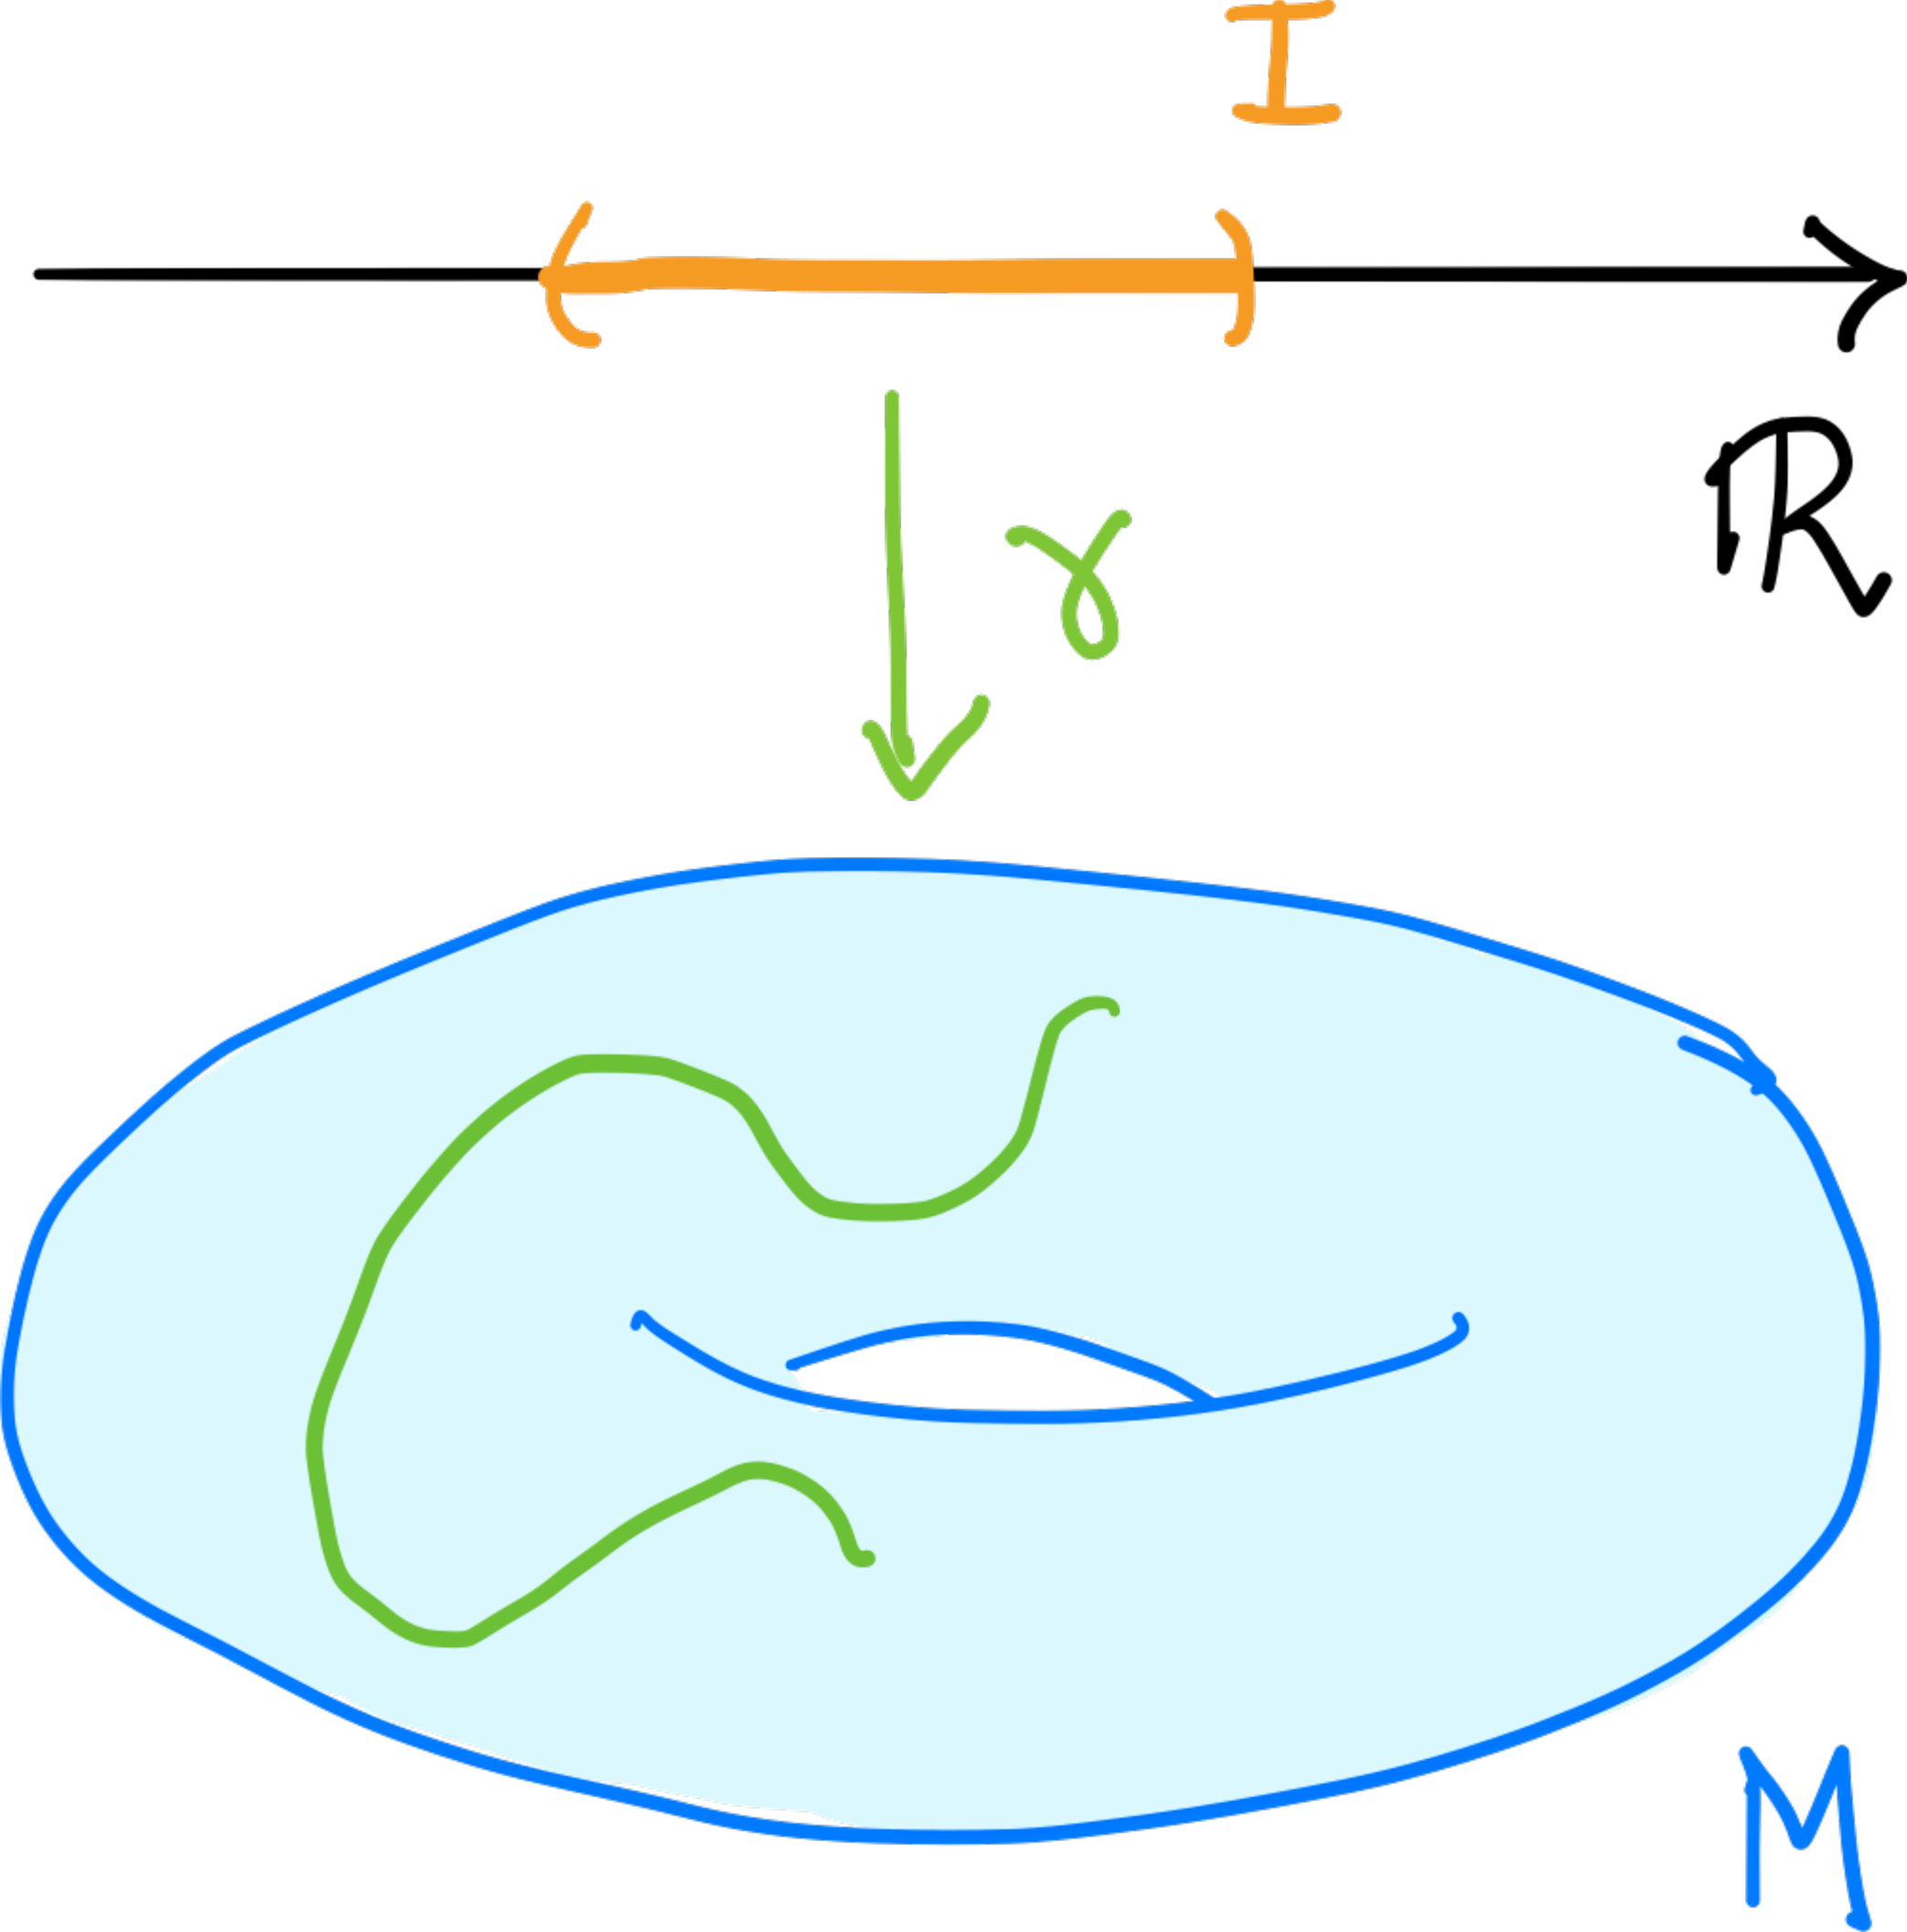
\includegraphics{2_2-curve-on-M.pdf}
\end{marginfigure}

Fix $t\in(a,b)$. 
A priori we have two different ways to define the \emph{velocity vector of $\gamma$ at a time $t$}, that is, an element $\gamma'(t) \in T_{\gamma(t)}M$:
\begin{enumerate}[(i)]
  \item We can define a derivation on $C^\infty(M)$ at $\gamma(t)$ by setting
  \begin{equation}\label{eq:tg_curve_der}
    \gamma'(t) (f) := (f\circ\gamma)'(t), \quad f\in C^\infty(M).
  \end{equation}
  \begin{exercise}
    Show that this is indeed a derivation on $C^\infty(M)$.
  \end{exercise}
  \item If we think of $\gamma$ as a smooth map between manifolds, we can define the tangent vector via the differential $d\gamma_t$:
  \begin{equation}\label{eq:tg_curve_diff}
    \gamma'(t):= d\gamma_t\left(\frac{\partial}{\partial t}\Big|_t\right) \in T_{\gamma(t)}M.
  \end{equation}
\end{enumerate}

Do these definition agree?
One way to check is to pick a chart $\varphi: U \to \varphi(U)$ in a neighbourhood of $\gamma(t)$, and compare the expressions in local coordinates. Let $(x^i)$ denote the coordinates of $\varphi$ and define the curves $\gamma^i := x^i \circ \gamma : I\to\R$.
Let's focus on~\eqref{eq:tg_curve_der}. By definition, $\gamma'(t)(x^i) = (x^i\circ\gamma)'(t) = (\gamma^i)'(t)$, therefore by Proposition~\ref{prop:basis_TpM} we get
\begin{equation}\label{eq:tg_curve_vec}
  \gamma'(t) = %\sum_{i=1}^m
    \gamma'(t)(x^i) \frac{\partial}{\partial x^i}\Big|_{\gamma(t)}.
\end{equation}
\begin{exercise}
  Show that applying Proposition~\ref{prop:DiffCoords} to~\eqref{eq:tg_curve_diff} leads to the same formula as~\eqref{eq:tg_curve_vec}.
\end{exercise}

\begin{figure*}[htp]
  \centering
  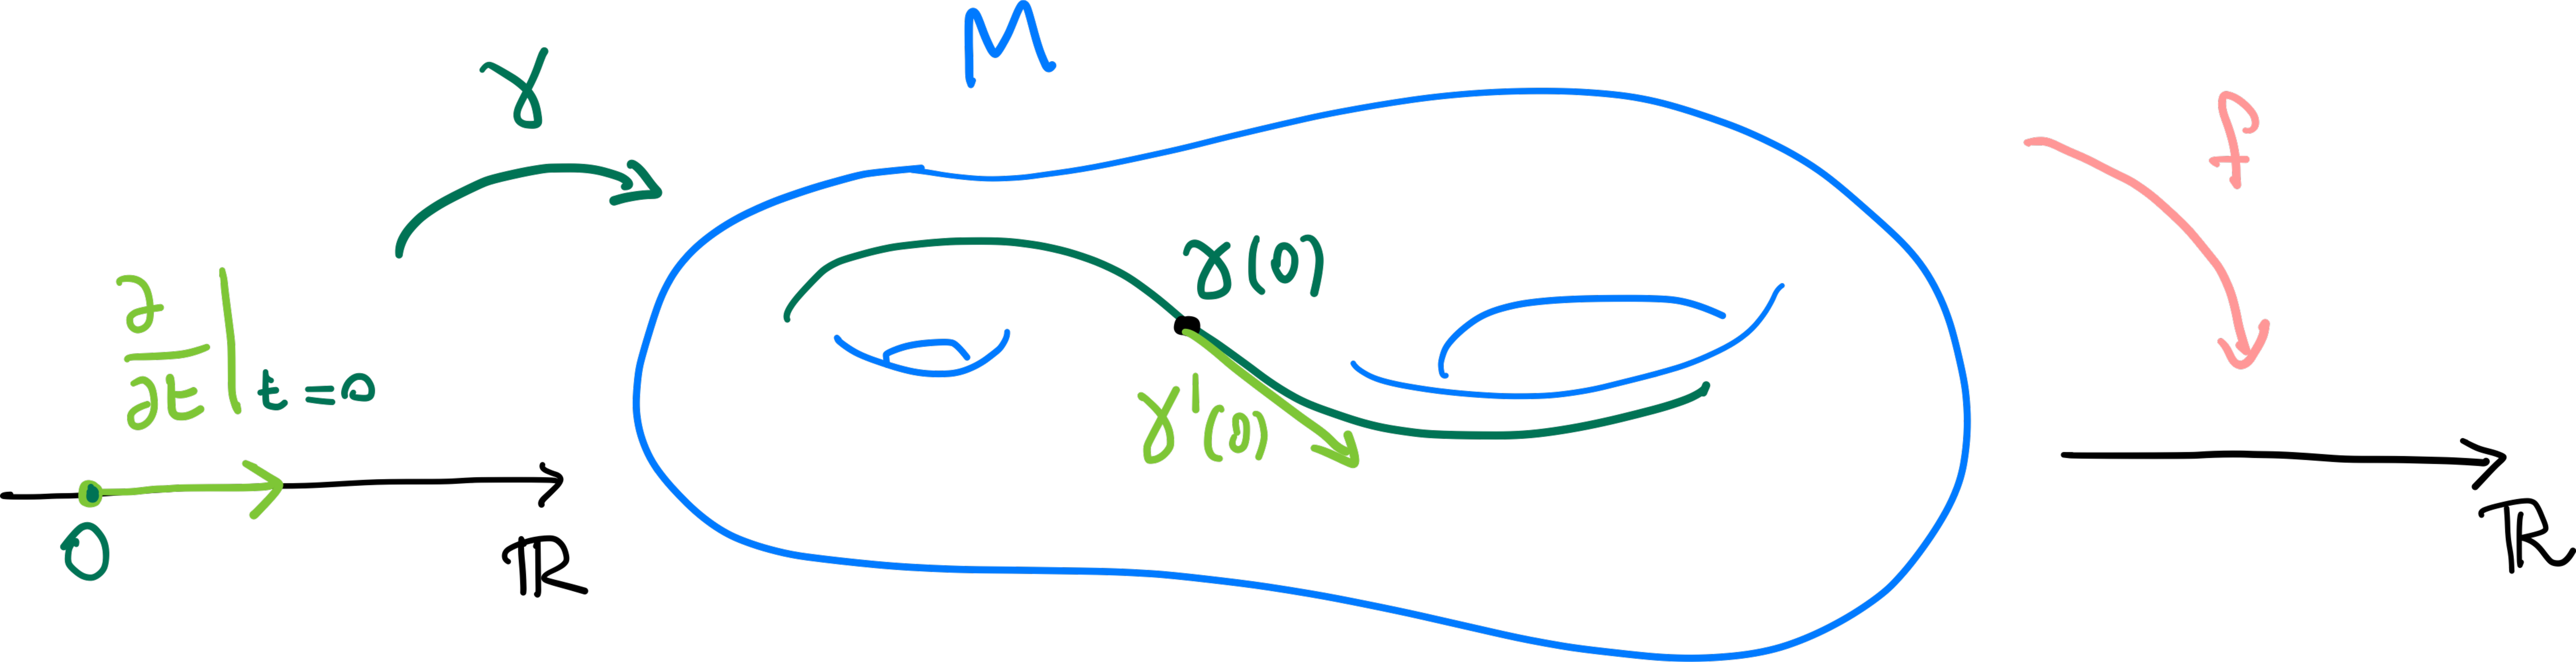
\includegraphics{2_5-v_cur_full.pdf}
  \caption{The velocity of a curve}
  \label{fig:2_5-v_cur_full}
\end{figure*}

But how can this mapping between curves and tangent vector be well--defined?
Surely, there must be multiple curves with the same speed at a point which differ outside a neighbourhood of the point.

\begin{lemma}\label{lem:equiv_tg_curves}
  Let $M$ be a smooth manifolds and $\gamma, \delta : (-\epsilon, \epsilon) \to M$ two smooth curves with $\gamma(0) = \delta(0)$. Then, $\gamma'(0) = \delta'(0)$ as elements of $T_{\gamma(0)}M$ if and only if for some (and thus any) chart $\varphi:U\to\varphi(U)$, $\gamma(0)\in U$, we have $(\varphi\circ \gamma)'(0) = (\varphi\circ\delta)'(0)$.
\end{lemma}
\begin{proof}
  Let $(x^i)$ denote the coordinates of $\varphi$. The condition $(\varphi\circ \gamma)'(0) = (\varphi\circ\delta)'(0)$ is equivalent as stating that $(\gamma^i)'(0) = (\delta^i)'(0)$, where $\gamma^i = x^i\circ\gamma$ and $\delta^i=x^i\circ\delta$. Then, the claim follows from~\eqref{eq:tg_curve_vec} and the fact that $\left\{\frac{\partial}{\partial x^i}\big|_{\gamma(0)}\right\}$ is a basis of $T_{\gamma(0)}M$.
\end{proof}

This seems to follow a pattern: until now, all the definitions of tangent vectors where in terms of classes of equivalence.
And it would seem reasonable to identify curves that that have the same tangent vector at $0$.
There is still a potential problem, though: we don't yet know if \emph{every} tangent vector can be written as the velocity vector of a curve.

\begin{theorem}
  Let $M$ be a smooth $n$-manifold, let $p\in M$ and let $v\in T_pM$.
  There exists a smooth curve $\gamma: (-\epsilon,\epsilon) \to M$ such that $\gamma'(0) = v$.
\end{theorem}
\begin{proof}
  Let $\varphi:U\to\varphi(U)$ be a chart about $p$ such that $\varphi(p)=0$.
  Let $(x^i)$ denote the coordinates of $\varphi$, as usual, and assume that
  \begin{equation}
    v = \sum_{i=1}^n a^i \frac{\partial}{\partial x^i}\Big|_p, \qquad a^i \in\R.
  \end{equation}
  For $\epsilon$ small enough, by continuity the vector $(ta^1, \ldots, ta^n) \in \varphi(U)$ for all $|t|<\epsilon$. Therefore, the curve
  \begin{equation}
    \gamma: (-\epsilon, \epsilon) \to M, \quad \gamma(t):=\varphi^{-1}(ta^1, \ldots, ta^n),
  \end{equation}
  is well-defined, smooth, satisfies $\gamma(0) = p$ and, by~\eqref{eq:tg_curve_vec}, $\gamma'(0) = v$.
\end{proof}

\begin{marginfigure}
  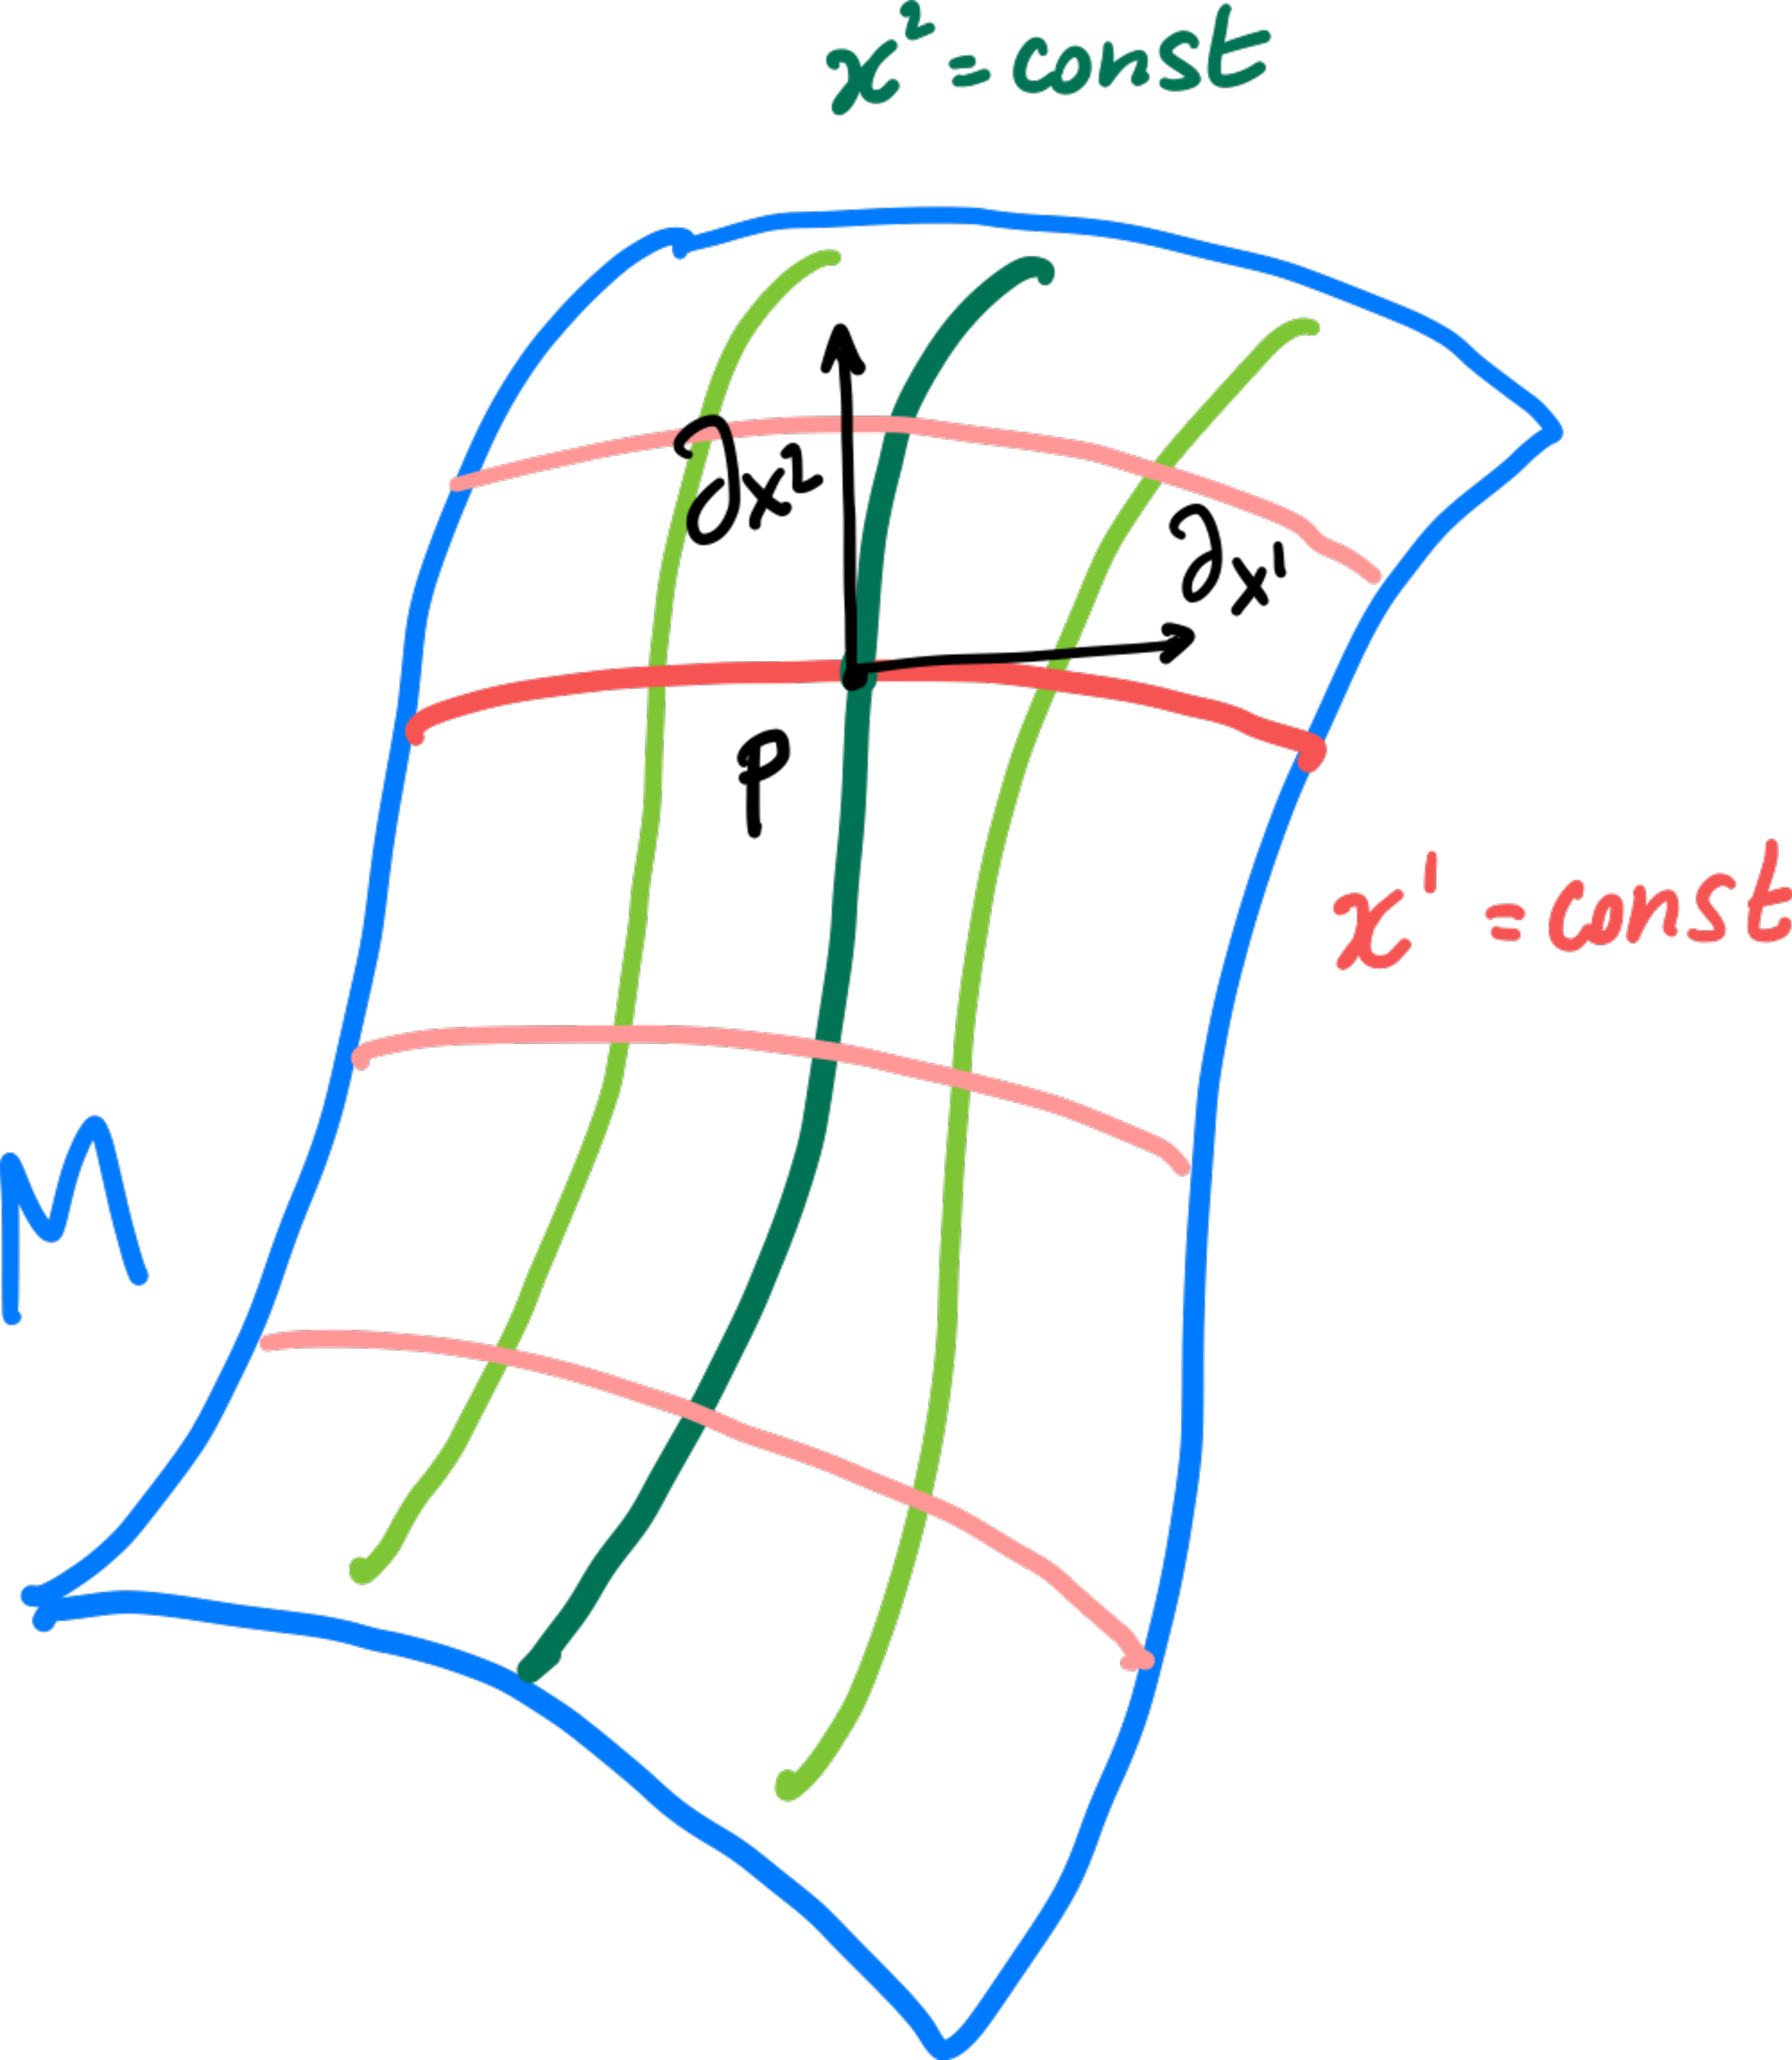
\includegraphics{2_4-v_cur.pdf}
  \caption{With this definition, the coordinate tangent vectors $\partial_{x^i}\in T_p M$ become the tangent vectors defined by the curve \[t \mapsto \varphi^{-1}(x^1(p), \ldots, {x^i(p) + t}, \ldots, x^n(p)).\]}
  \label{fig:2_4-v_cur}
\end{marginfigure}
This means that we can actually give an alternative definition of $T_xM$ in terms of tangents to curves:
\begin{definition}\label{def:tg:ascurvespeed}
  A tangent vector at $p\in M$ is an equivalence class of smooth curves $\gamma:(-\epsilon, \epsilon)\to M$ such that $\gamma(0)=p$, where $\gamma\sim\delta$ if and only if $(\varphi\circ \gamma)'(0) = (\varphi\circ\delta)'(0)$ for some chart $\varphi$ centred about $p$ (see Lemma~\ref{lem:equiv_tg_curves}).
\end{definition}

In fact, it is possible to start the whole tangent space discussion with the above definition. In that case, you would first need to prove Exercise~\ref{exe:vsstruct} and endow $T_pM$ with a vector space structure\footnote{To get the analogue result as Proposition~\ref{prop:basis_TpM}}.

To conclude this part, the next proposition shows that velocity vectors behave well under composition with smooth maps and give us a direct, explicit and effective way to compute differentials.

\begin{proposition}\label{prop:curves_deriv}
  Let $F:M\to N$ b a smooth map between smooth manifolds and $\gamma:I\to M$ a smooth curve in $M$.
  Then
  \begin{equation}
    d F_{\gamma(t)} (\gamma'(t)) = (F\circ\gamma)'(t).
  \end{equation}
\end{proposition}
\begin{proof}
  We are going to use~\eqref{eq:tg_curve_diff} as definition of $\gamma'(t)$.
  Applying the chain rule we obtain:
  \begin{align}
    d F_{\gamma(t)} (\gamma'(t))
    &= d F_{\gamma(t)} \circ d\gamma_t\left(\frac{\partial}{\partial t}\Big|_t\right) \\
    &= d (F\circ\gamma)_t \left(\frac{\partial}{\partial t}\Big|_t\right) \\
    &= (F\circ\gamma)'(t).
  \end{align}
\end{proof}

\begin{exercise}
  Give an alternative proof of Proposition~\ref{prop:curves_deriv} using~\eqref{eq:tg_curve_der} as definition for $\gamma'(t)$.\\
 \textit{\small Hint: use the definitions to rewrite the formula in different ways.}
\end{exercise}

\section{The tangent bundle}\label{sec:tangentbundle}

Instead of working separately with the various tangent spaces, we can ``glue'' them together into a big manifold.

\begin{marginfigure}
  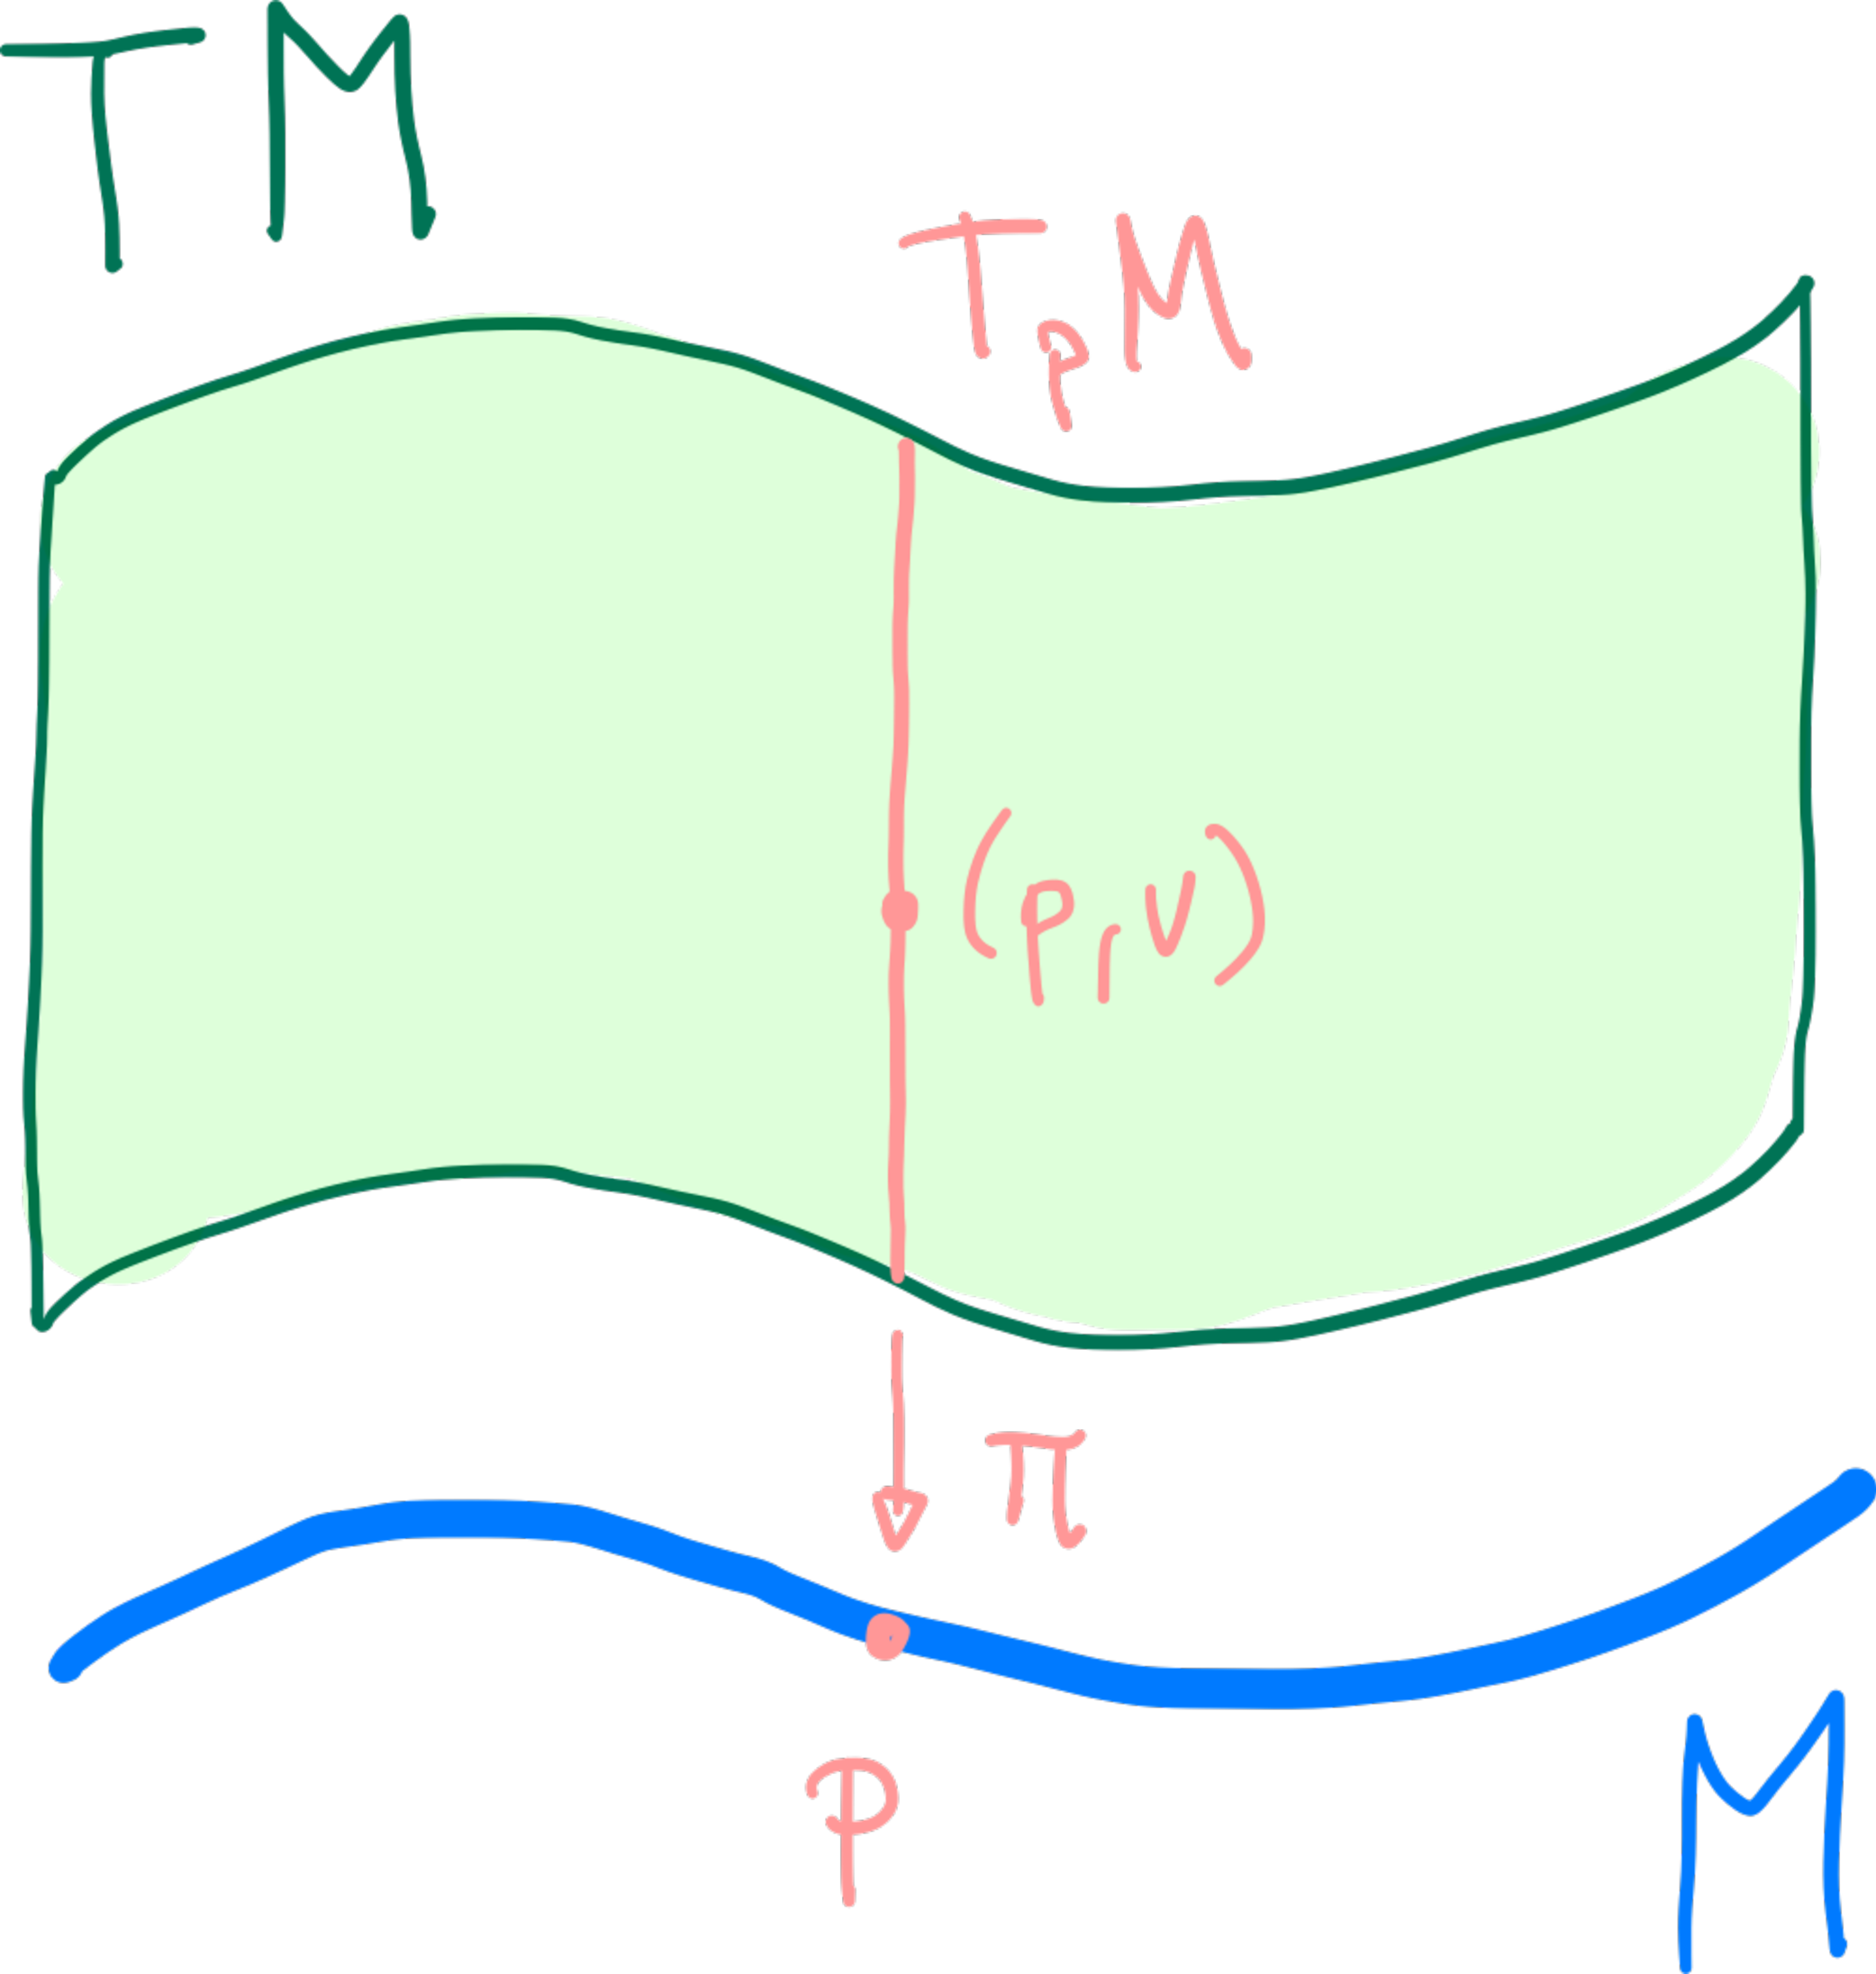
\includegraphics{2_6-tg_bdl_proj.pdf}
\end{marginfigure}
\begin{definition}
  The \emph{tangent bundle} $TM$ of $M$ is the disjoint union of the tangent spaces
  \begin{equation}
    TM := \bigsqcup_{p\in M}\left(\{p\}\times T_pM\right)
       = \{(p,v) \;\mid\; p\in M,\, v\in T_pM\}.
  \end{equation}  
\end{definition}

Elements in $TM$ are pairs\footnote{We will often abuse notation and identify $T_pM$ with with its image under the canonical injection $v\mapsto(p,v)$ and use interchangeably any of the notations $v$, $v_p$ or $(p,v)$ for a vector in $T_pM$ (depending on how much emphasis we need to put on the base point).} $(p,v)$ of a \emph{base point} $p\in M$ and a \emph{tangent vector} $v\in T_pM$.

To the tangent bundle we associate a surjective map $\pi:TM \to M$, the \emph{projection (onto the base)}, which sends each vector in a tangent space to the point at which it is tangent, that is, $\pi(p,v) = p$.
The second component of the pre-image $\pi^{-1}(\{p\}) = \{p\}\times T_pM$, that is $T_pM$ itself, is called the \emph{fibre} over $p\in M$.
We will come back to this later on once we talk about vector bundles.

\begin{example}
  Let $M\subset \R^n$ be an an open set.
  We can identify $TM$ in a natural way with $M\times\R^n$.
  Since $M\times\R^n \subset \R^{2n}$ and thus is a manifold, we can equip the tangent bundle $TM$ with the structure of a manifold induced by this identification.
\end{example}

As it turns out, this is a particular instance of a more general fact.

\begin{theorem}\label{thm:tgbdlsmoothmfld}
  Let $M$ be a smooth $n$-manifold.
  The smooth structure on $M$ naturally\footnote{In the sense that its definition does not require to make any arbitrary choices.} induces a smooth structure on $TM$, making $TM$ into a smooth manifold of dimension $2n$.
  Moreover, the map $\pi: TM \to M$ is smooth.
\end{theorem}
\begin{proof}
  \marginnote[1em]{In this proof you can see instances of a typical abuse of notation: in the expressions $\widetilde x^i(x)$ we think of the $\widetilde x^i$ as coordinate functions but we think of the $x$ as representing a point in $\varphi(U\cap V)$.}
  \newthought{Step 1: extending charts from $M$ to $TM$.}
  Given a chart $(U,\varphi)$ about $p\in M$, the preimage $\pi^{-1}(U) \subset TM$ is the set of all tangent vectors to $M$ at points of $U$.
  If $(x^i)$ denotes the coordinate functions of $\varphi$, we can define a map $\widetilde\varphi : \pi^{-1}(U) \to \varphi(U)\times\R^n \subset \R^{2n}$ by
  \marginnote{Keep in mind that \begin{equation}\nonumber
    \pi^{-1}(U)= TU = \bigsqcup T_p U \subset \bigsqcup T_p M=TM.
  \end{equation}}
  \begin{align}\label{eq:nat_coords}
    \widetilde\varphi\left(v^i \frac{\partial}{\partial x^i}\Big|_p\right) := \left(x^1(p), \ldots, x^n(p), v^1, \ldots, v^n\right).
  \end{align}
  Since $\widetilde\varphi$ can be explicitly inverted as $\widetilde\varphi^{-1}\left(x^1, \ldots, x^n, v^1, \ldots, v^n\right) = v^i \frac{\partial}{\partial x^i}\Big|_{\varphi^{-1}(x)}$, it defines a bijection onto its image.

  \newthought{Step2: compatibility of the extended charts.}
  Suppose we have two smooth charts $(U,\varphi)$, $(V,\psi)$ for $M$ with the respective local coordinates $(x^i)$ and $(y^i)$.
  Let $(\pi^{-1}(U),\widetilde\varphi)$, $(\pi^{-1}(V),\widetilde\psi)$ be their extension\footnote{These are called \emph{bundle charts}.} to $TM$ as in the previous step.
  By construction\footnote{They are both homeomorphisms.}, both $\widetilde\varphi(\pi^{-1}(U)\cap\pi^{-1}(V)) = \varphi(U\cap V)\times\R^n$ and $\widetilde\psi(\pi^{-1}(U)\cap\pi^{-1}(V)) = \psi(U\cap V)\times\R^n$ are open in $\R^{2n}$.
  Moreover, we can take advantage of Remark~\ref{rmk:chg_coords} to write explicitly the transition map  $\widetilde\psi\circ\widetilde\varphi^{-1}: \varphi(U\cap V)\times\R^n \to \psi(U\cap V)\times\R^n$ as
  \begin{align}
    \widetilde\psi\circ&\widetilde\varphi^{-1}\left(x^1, \ldots, x^n, v^1, \ldots, v^n\right) \\
    &=\left(y^1(p),\ldots, y^n(p), \frac{\partial y^1}{\partial x^j}(p) v^j, \ldots, \frac{\partial y^n}{\partial x^j}(p) v^j\right),
  \end{align}
  where $p = \phi^{-1}(x)$, which is clearly smooth.
  
  \begin{figure*}[htp]
    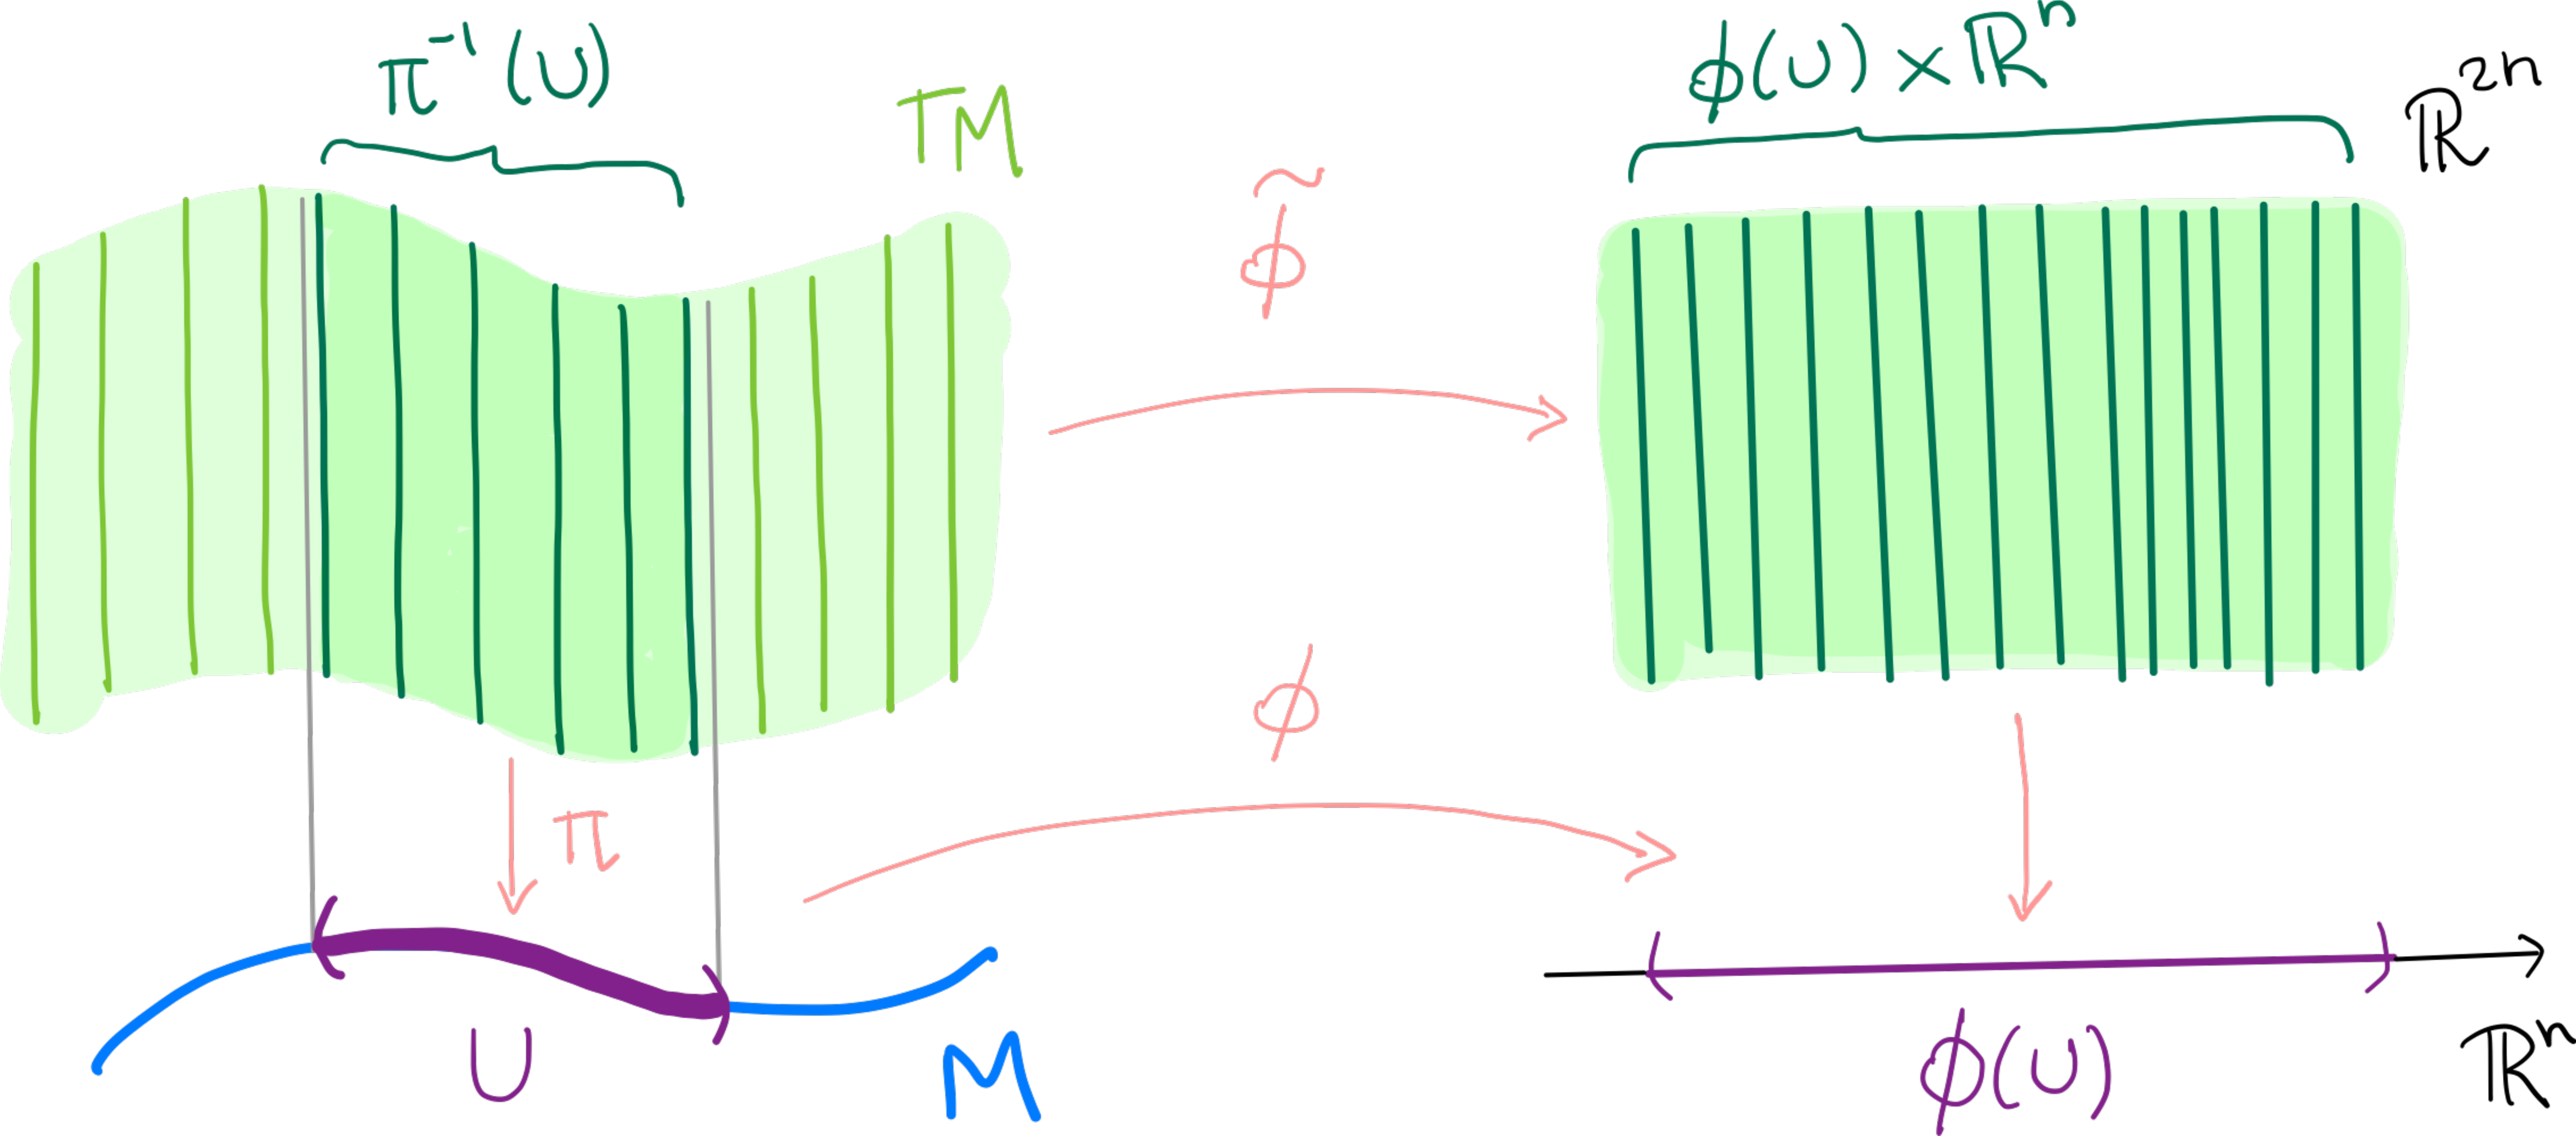
\includegraphics{2_7-tg_bdl_coord.pdf}
    \caption{Coordinates for the tangent bundle}
  \end{figure*}
  
  \newthought{Step3: $TM$ is a manifold.}
  With the procedure delineated above, a countable smooth atlas $\{(U_i, \varphi_i)\}$ of $M$ induces a countable atlas $\{(\pi^{-1}(U_i), \widetilde\varphi_i)\}$ of $TM$.
  First of all, $\{(\pi^{-1}(U_i)\}$ provides a countable covering of $TM$.
  We need to show that the topology induced by those charts is Hausdorff and second countable.
  
  Let $(p_1, v_1), (p_2, v_2) \in TM$ be different points: either $p_1\neq p_2$, or $p_1 = p_2$ and $v_1 \neq v_2$.
  \begin{itemize}
    \item In the first case, there are disjoint open sets $V_1, V_2 \subset U_i$ (for some $i$) containing respectively $p_1$ and $p_2$.
    Then $\widetilde\varphi_i^{-1}(\varphi_i(V_1)\times\R^n)$ and $\widetilde\varphi_i^{-1}(\varphi_i(V_2)\times\R^n)$ are disjoint open sets containing respectively $(p_1, v_1)$ and $(p_2, v_2)$.
    \item In the second case, $p=p_1=p_2$ but there are disjoint open sets $V_1,V_2\subset \R^n$ containing $v_1$ and $v_2$ respectively;
    again, the preimages $\widetilde\varphi_i^{-1}(\varphi_i(U_i)\times V_1)$ and $\widetilde\varphi_i^{-1}(\varphi_i(U_2)\times V_2)$ (for some $i$ such that $p\in U_i$) are disjoint open sets containing respectively $(p_1, v_1)$ and $(p_2, v_2)$.
  \end{itemize}

  The countable basis $\{U_j\}$ is a countable basis for the topology of $M$ (which is second countable), taking a countable basis $\{W_k\}$ for the topology of $\R^n$, we can define a countable basis for $TM$ as $\{\widetilde\varphi^{-1}((U_i\cap U_j)\times W_k)\}$.
  The charts defined above make $TM$ automatically euclidean of dimension $2n$.

  \begin{exercise}
    This part of the proof seems unnecessarily detailed.
    Can you simplify it using Lemma~\ref{lem:manifold_chart}?
  \end{exercise}

  \newthought{Step4: $\pi$ is smooth.} With respect to the charts $(U,\varphi)$ for $M$ and $(\pi^{-1}(U), \widetilde\varphi)$ for $TM$, the coordinate representation of $\pi$ is $\pi(x,v) = x$.
\end{proof}

The coordinates $(x^i, v^i)$ defined by~\eqref{eq:nat_coords} are called \emph{natural (or canonical) coordinates}.

\begin{exercise}
  Let $f:M\to N$ be a smooth map between smooth manifolds.
  Show that its differential $df: TM \to TN$ is a smooth map between smooth manifolds (the respective tangent bundles).\\
  \textit{\small Hint: use the natural differentiable structure on the tangent bundle described above and the definition of smooth map.}
\end{exercise}

\begin{remark}
  In classical mechanics, the configuration space is usually a manifold $M$.
  The tangent bundle $TM$ corresponds to the state space, that is, the space of configurations and velocities. In symbols $x=(q,v)$ is a pair of a configuration $q = \pi(x)$ and a velocity $v\in T_q M$.
  It turns out that the Lagrangian is a smooth function on $TM$.
\end{remark}

\section{Vector bundles}\label{sec:vectorbundle}

What we have seen here is our first example of vector bundle, which is just a way to call a vector space depending continuously (or smoothly) on some parameters, for example points on a manifold.

\begin{definition}\label{def:vector_bundle}
  A \emph{vector bundle of rank $r$} on a manifold $M$ is a manifold $E$ together with a smooth surjective map $\pi : E \to M$ such that, for all $p\in M$, the following properties hold:
  \begin{enumerate}[(i)]
    \item the \emph{fibre over $p$}, $E_p := \pi^{-1}(p)$, has the structure of vector space of dimension $r$;
    \item there is a neighbourhood $U\subset M$ of $p$ and a diffeomorphism $\varphi: \pi^{-1}(U) \to U \times \R^r$ such that
    \begin{enumerate}
      \item $\pi_1 \circ \varphi = \pi$ where $\pi_1: U\times\R^r\to U$ is the projection on the first factor,
      \item for all $q\in U$, $\varphi\big|_{E_q} : E_q \to \{q\}\times \R^r$ is an isomorphism of vector spaces.
    \end{enumerate}
  \end{enumerate}

  The space $E$ is called the \emph{total space}, the manifold $M$ is the \emph{base space}, $\pi$ its projection and each of the maps $\varphi$ is called \emph{local trivialisation}.

  If there exists a trivialisation defined on the whole manifold, that is a map $\varphi: M \to M\times \R^r$, such map is called \emph{global trivialisation} and the vector bundle is said to be \emph{trivialisable}.
\end{definition}

\begin{example}
  \begin{itemize}
    \item A simple example of vector bundle of rank $r$ over a manifold $M$ is the product space $E = M\times \R^r$ itself with the projection on the first component $\pi_1: E\to M$.
    In this case the bundle is clearly trivialisable.
    \item The tangent bundle $TM$ with its projection to the base $\pi:TM\to M$ is a vector bundle.
    In this case the fibres are the tangent spaces $\pi^{-1}(p) = T_pM$. 
    If the tangent bundle of a manifold is trivalisable, then its base manifold is said to be \emph{parallelisable}.
    \item If $\pi_i: E_i\to M_i$, $i=1,2$, are vector bundles, then $\pi = (\pi_1, \pi_2): E_1\times E_2 \to M_1\times M_2$ is another vector bundle whose fibres are the product of the fibres of the two original bundles.
    A particular example of this is the tangent bundle $T(M_1\times M_2)$, which is diffeomorphic to $TM_1 \times TM_2$.
    \item Other examples will appear throughout the course.
  \end{itemize}
\end{example}

\begin{exercise}
  Show that $\dim(E) = \dim(M) + r$.
\end{exercise}

\begin{exercise}
  Show that if $\pi:E\to M$ is a vector bundle and $U\subset M$ is an open set, then $\pi\big|_{\pi^{-1}(U)}: \pi^{-1}(U) \to U$ is a vector bundle of the same rank.
\end{exercise}

\begin{example}
  Let $\pi:E \to M$ be a vector bundle of rank $r$.
  Assume that $E$ itself is the base space of another vector bundle $\pi_1: E_1\to E$ of rank $s$.
  Then $\pi\circ\pi_1: E_1 \to M$ is a vector bundle of rank $r+s$ called the \emph{composite bundle}. Indeed, if $\varphi:\pi^{-1}(U)\to U\times\R^r$ is a bundle diffeomorphism for $E$ over $U\subset M$ and $\varphi_1:\pi_1^{-1}(U_1)\to U_1\times\R^s$ is a bundle diffeomorphism for $E_1$ over $U_1\subset E$ such that $V := \pi(U_1)\cap U\neq \emptyset$, then
  \begin{equation}
    \Psi:=(\varphi\circ\pi_1, \varphi_1): (\pi\circ\pi_1)^{-1}(V)\to (U\times\R^r)\times (U_1\times\R^s)
  \end{equation}
  is a bundle diffeomorphism for $\pi\circ\pi_1$ over $W$.

  A particular example of this is the tangent bundle of the tangent bundle: if $M$ is a $n$-manifold, its tangent bundle $TM$ is a $2n$-manifold, and its tangent bundle $T(TM)$ is a vector bundle over $M$ of rank $3n$.
\end{example}

To compare vector bundles is useful to define the following concept.
\begin{definition}
  A \emph{isomorphims} between two vector bundles $\pi_i: E_i \to M$, $i=1,2$, over the same base space $M$ is a homeomorphism $h:E_1 \to E_2$ which maps every fiber $\pi_1^{-1}(p)$ to the corresponding fiber $\pi_2^{-1}(p)$ by a linear isomorphism.
\end{definition}

Since an isomorphism preserves all the structure of a vector bundle, isomorphic bundles are often regarded as the same.

\begin{marginfigure}[-30em]
  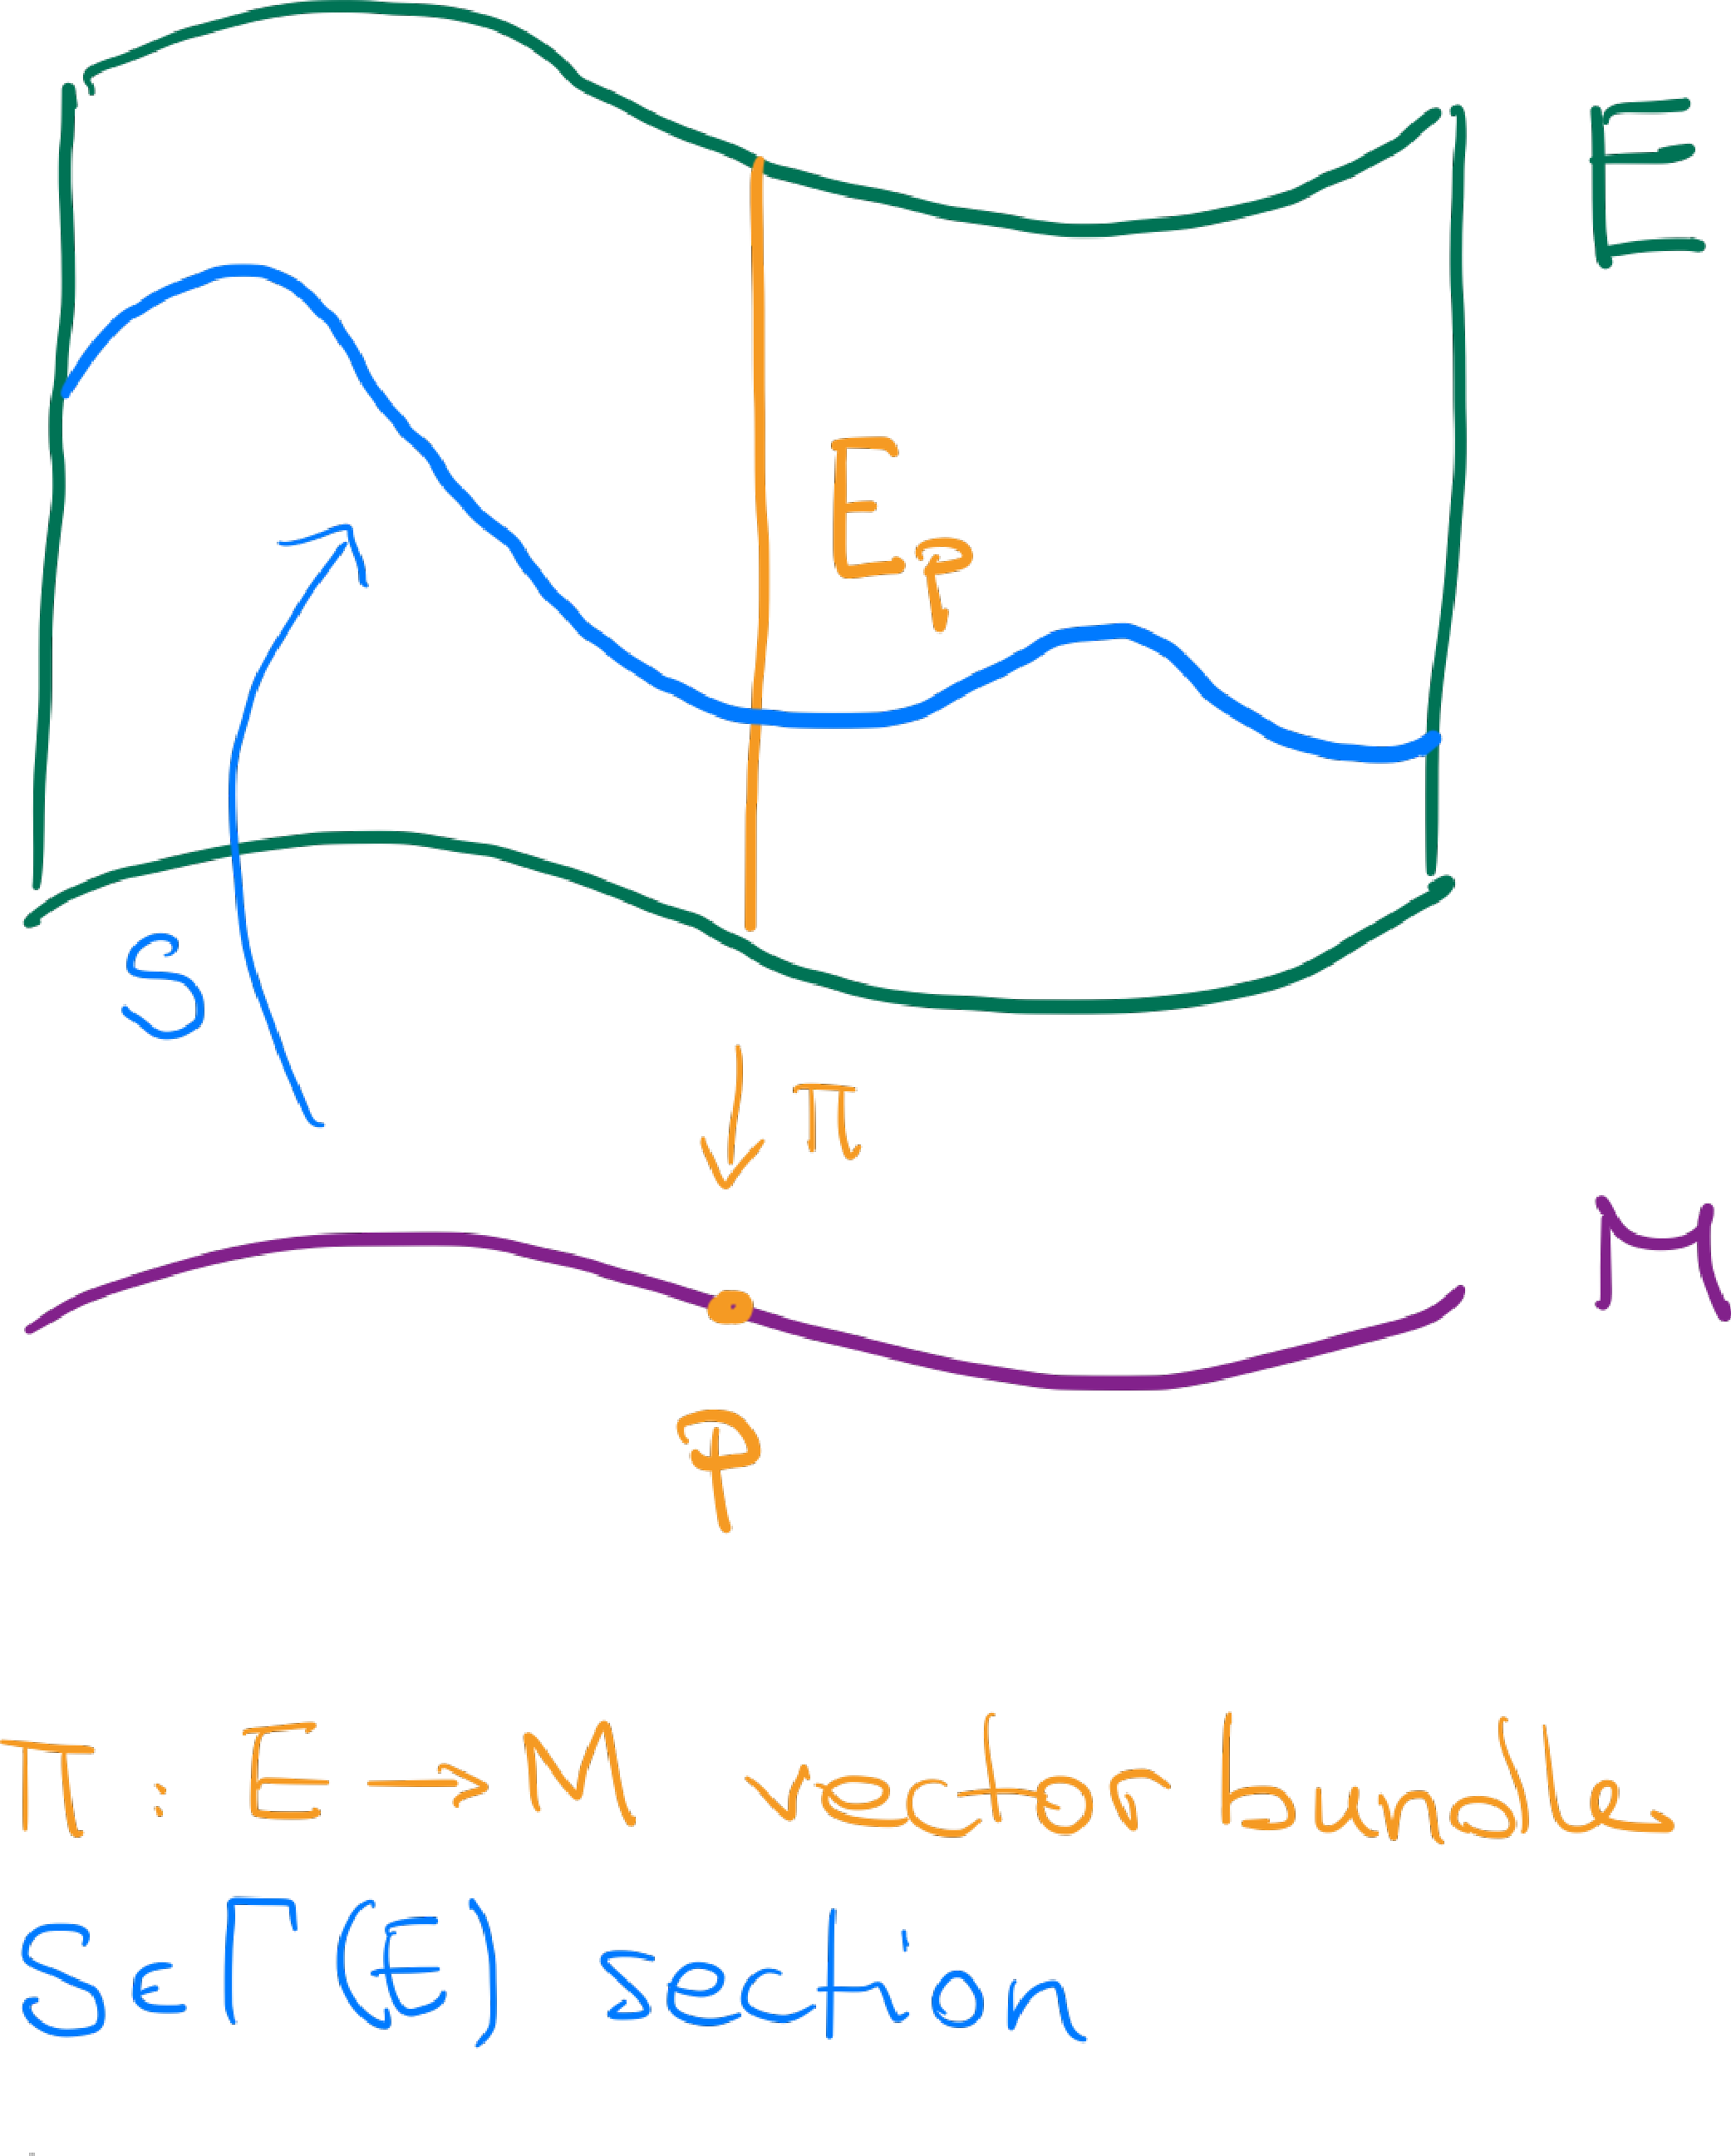
\includegraphics{2_7-bdl_section.pdf}
  \caption{A useful mnemonic to remember what is a section, is to imagine it as a cross-section of the bundle.}
\end{marginfigure}

\begin{definition}
  A \emph{section} of a vector bundle $\pi:E \to M$ is a smooth map $S:M \to E$ such that $\pi\circ S = \id_M$. We denote the set of all sections of $E$ by $\Gamma(E)$.
  
  If, in the definition, $M$ is replaced by $U\subset M$, the section is called \emph{local section}. The set of local sections on $U\subset M$ is denoted $\Gamma(E|_U)$.
\end{definition}

\begin{example}
  If $E = M\times \R^r$, $M\subset\R^n$, then for any smooth map $F: M\to\R^r$ we have a section $S\in\Gamma(E)$ defined by $S(p) = (p, F(p))$. This is a classical euclidean vector field: a map that associates vectors to points.
  \begin{marginfigure}
    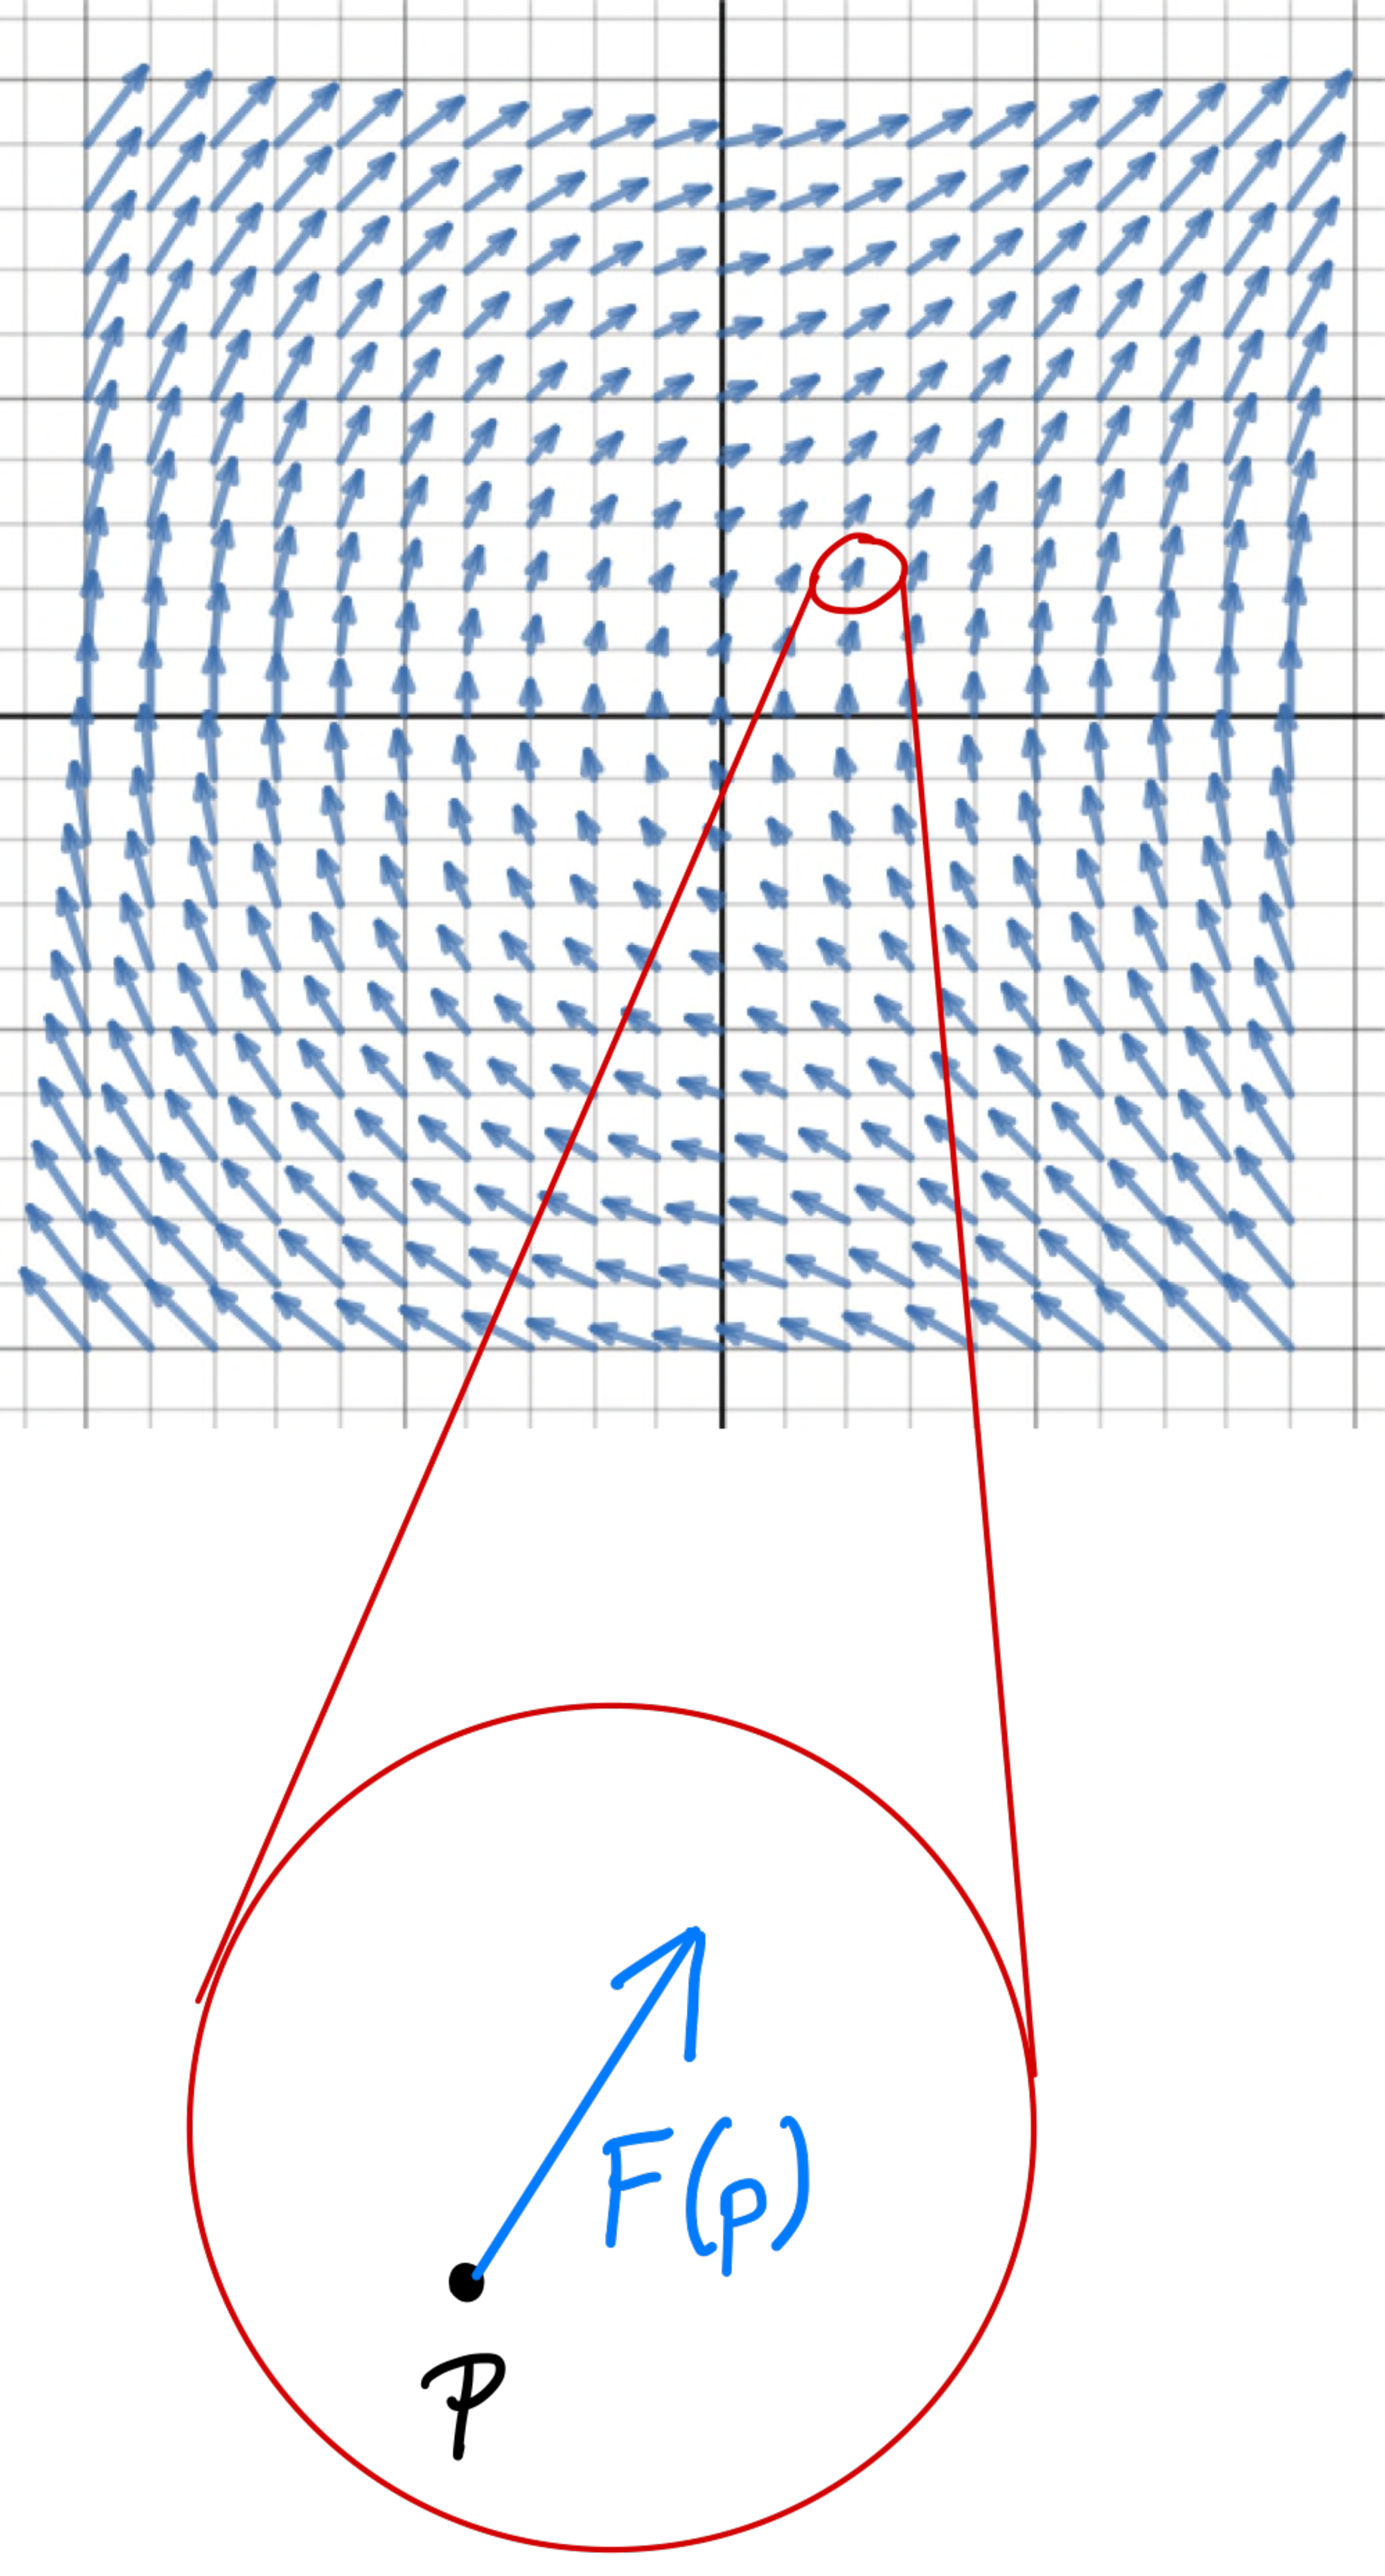
\includegraphics{2_9-vfield.pdf}
    \caption{A vector field ``attaches'' vectors to points.}
  \end{marginfigure}
  \noindent Notice, in particular, that functions $f\in C^\infty(M)$ are sections of the trivial bundle $M\times\R$.
\end{example}

One can sometimes distinguish non--isomorphic bundles by looking at the complement of their zero section: since any vector bundle isomorphism $h:E_1\to E_2$ must map the zero section of $E_1$ onto the zero section of $E_2$, the complements of the zero sections in $E_1$ and $E_2$ must be homeomorphic.

If the bundles are differentiable manifolds, then the definition of isomorphism nicely generalizes: they are \emph{diffeomorphic} if fibres are mapped to fibres diffeomorphically.

Even though, as we have seen, \emph{locally} $TM$ is diffeomorphic to $M\times\R^n$, this is not true in general with one exception.
\begin{exercise}\label{ex:trivialisable}
  Let $M$ be a smooth $n$-manifold that can be covered by a single smooth chart.
  Show that $TM$ is diffeomorphic to $M\times\R^n$ (without applying Proposition~\ref{prop:trivialisable}).
\end{exercise}

\begin{definition}
  A \emph{local frame} of a bundle $\pi:E\to M$ of rank $r$ is a family of $r$ local sections $(S_1, \ldots, S_r)\in\Gamma(E|_U)$ such that $(S_1(p), \ldots, S_r(p))$ is a basis for $E_p$ for all $p\in U$.
  If $U=M$ then $(S_1, \ldots, S_r)$ is called \emph{global frame}.
  Sometimes, the sections $S_j$ are called \emph{basis sections}.
\end{definition}

\begin{example}
  A chart on a $n$-manifold $M$ with local coordinates $(x^i)$ yields a local frame $\left\{\frac{\partial}{\partial x^1}, \ldots, \frac{\partial}{\partial x^n}\right\}$ of the tangent bundle $TM$.
\end{example}

In the spirit of what we have seen about the previous example, we have the following proposition.

\begin{proposition}
  Let $\pi:E \to M$ be a smooth vector bundle and $X:M\to E$ a section.
  If $(S_i)$ is a smooth local frame for $E$ over an open subset $U\subseteq M$, then $X$ is smooth on $U$ if an only if its component functions with respect to $(S_i)$ are smooth.
\end{proposition}
\begin{proof}
   Let $\varphi:\pi^{-1}(U) \to U\times\R^k$ be the local trivialization associated with the local frame $(S_i)$. Since $\varphi$ is a diffeomorphism, $X$ is smooth on $U$ if and only if $\varphi\circ X$ is smooth on $U$. If $(X^i)$ denote the component functions of $X$ with respect to $S_i$, then $\varphi\circ X (p) = (p, (X^1(p), \ldots, X^k(p)))$, so $\varphi\circ X$ is smooth if and only if the component functions $(X^i)$ are smooth.
\end{proof}

That is, given a local frame $\{S_1, \ldots, S_r\}\subset\Gamma(E|_U)$ of a vector bundle $\pi: E \to M$ we can express any section $X\in\Gamma(E)$ as a linear combination of elements of the frame:
\begin{equation}
  X = X^i S_i \quad\mbox{on }U,
\end{equation}
where $X^i\in C^\infty(U)$, $i=1,\ldots,r$.
Which was to be expected: after all, for each $p\in U\subset M$, the local frame is a basis for $E_p$.

\begin{proposition}\label{prop:trivialisable}
  A vector bundle $\pi: E\to M$ is trivialisable if and only if it admits a global frame.
\end{proposition}
\begin{proof}
  Let $\varphi: E \to M\times\R^r$ be a global trivialisation and $(e_1, \ldots, e_r)$ the canonical basis for $\R^r$.
  For $q\in M\times\R^r$, $(S_1(q), \ldots, S_r(q)) := \left(\varphi^{-1}\big|_q(e_1), \ldots, \varphi^{-1}\big|_q(e_r) \right)$ is a global frame for $E$ (why?).

  Conversely, let $(S_1, \ldots, S_r)$ be a global frame for $E$. Then
  \begin{equation}
    \varphi: E \to M\times\R^r, \quad
    \left(p, v^i S_i(p)\right) \mapsto \left(p, (v^1, \ldots, v^r)\right),
  \end{equation}
  is a global trivialisation for $E$.
\end{proof}

\begin{example}
  The cylinder $E = \bS^1\times\R$ is a trivialisable vector bundle with $\pi:E\to \bS^1$.
  Incidentally, the cylinder is isomorphic to $TS^1$ (why?).
\end{example}

A useful generalization of vector bundles, which we will not discuss in the course, is the locally trivial fiber bundle, where $\R$ is replaced by a more general manifold.

\section{Submanifolds}

With differentials of smooth functions at hand, we are ready to discuss submanifolds: smaller manifolds sitting inside larger ones.

\begin{definition}
  Let $M^m$ and $N^n$ be differentiable manifolds and $F:M\to N$ a $C^1$ function.
  \begin{itemize}
    \item $F$ is an \emph{immersion} if $dF_p$ is injective for all $p\in M$ ($\Rightarrow\; m\leq n$);
    \item $F$ is a \emph{submersion} if $dF_p$ is surjective for all $p\in M$ ($\Rightarrow\; m\geq n$);
    \item $F$ is an \emph{embedding} if $F$ is an injective immersion that is also a homeomorphism onto its range $F(M)\subset N$.
  \end{itemize}
\end{definition}
\begin{marginfigure}
  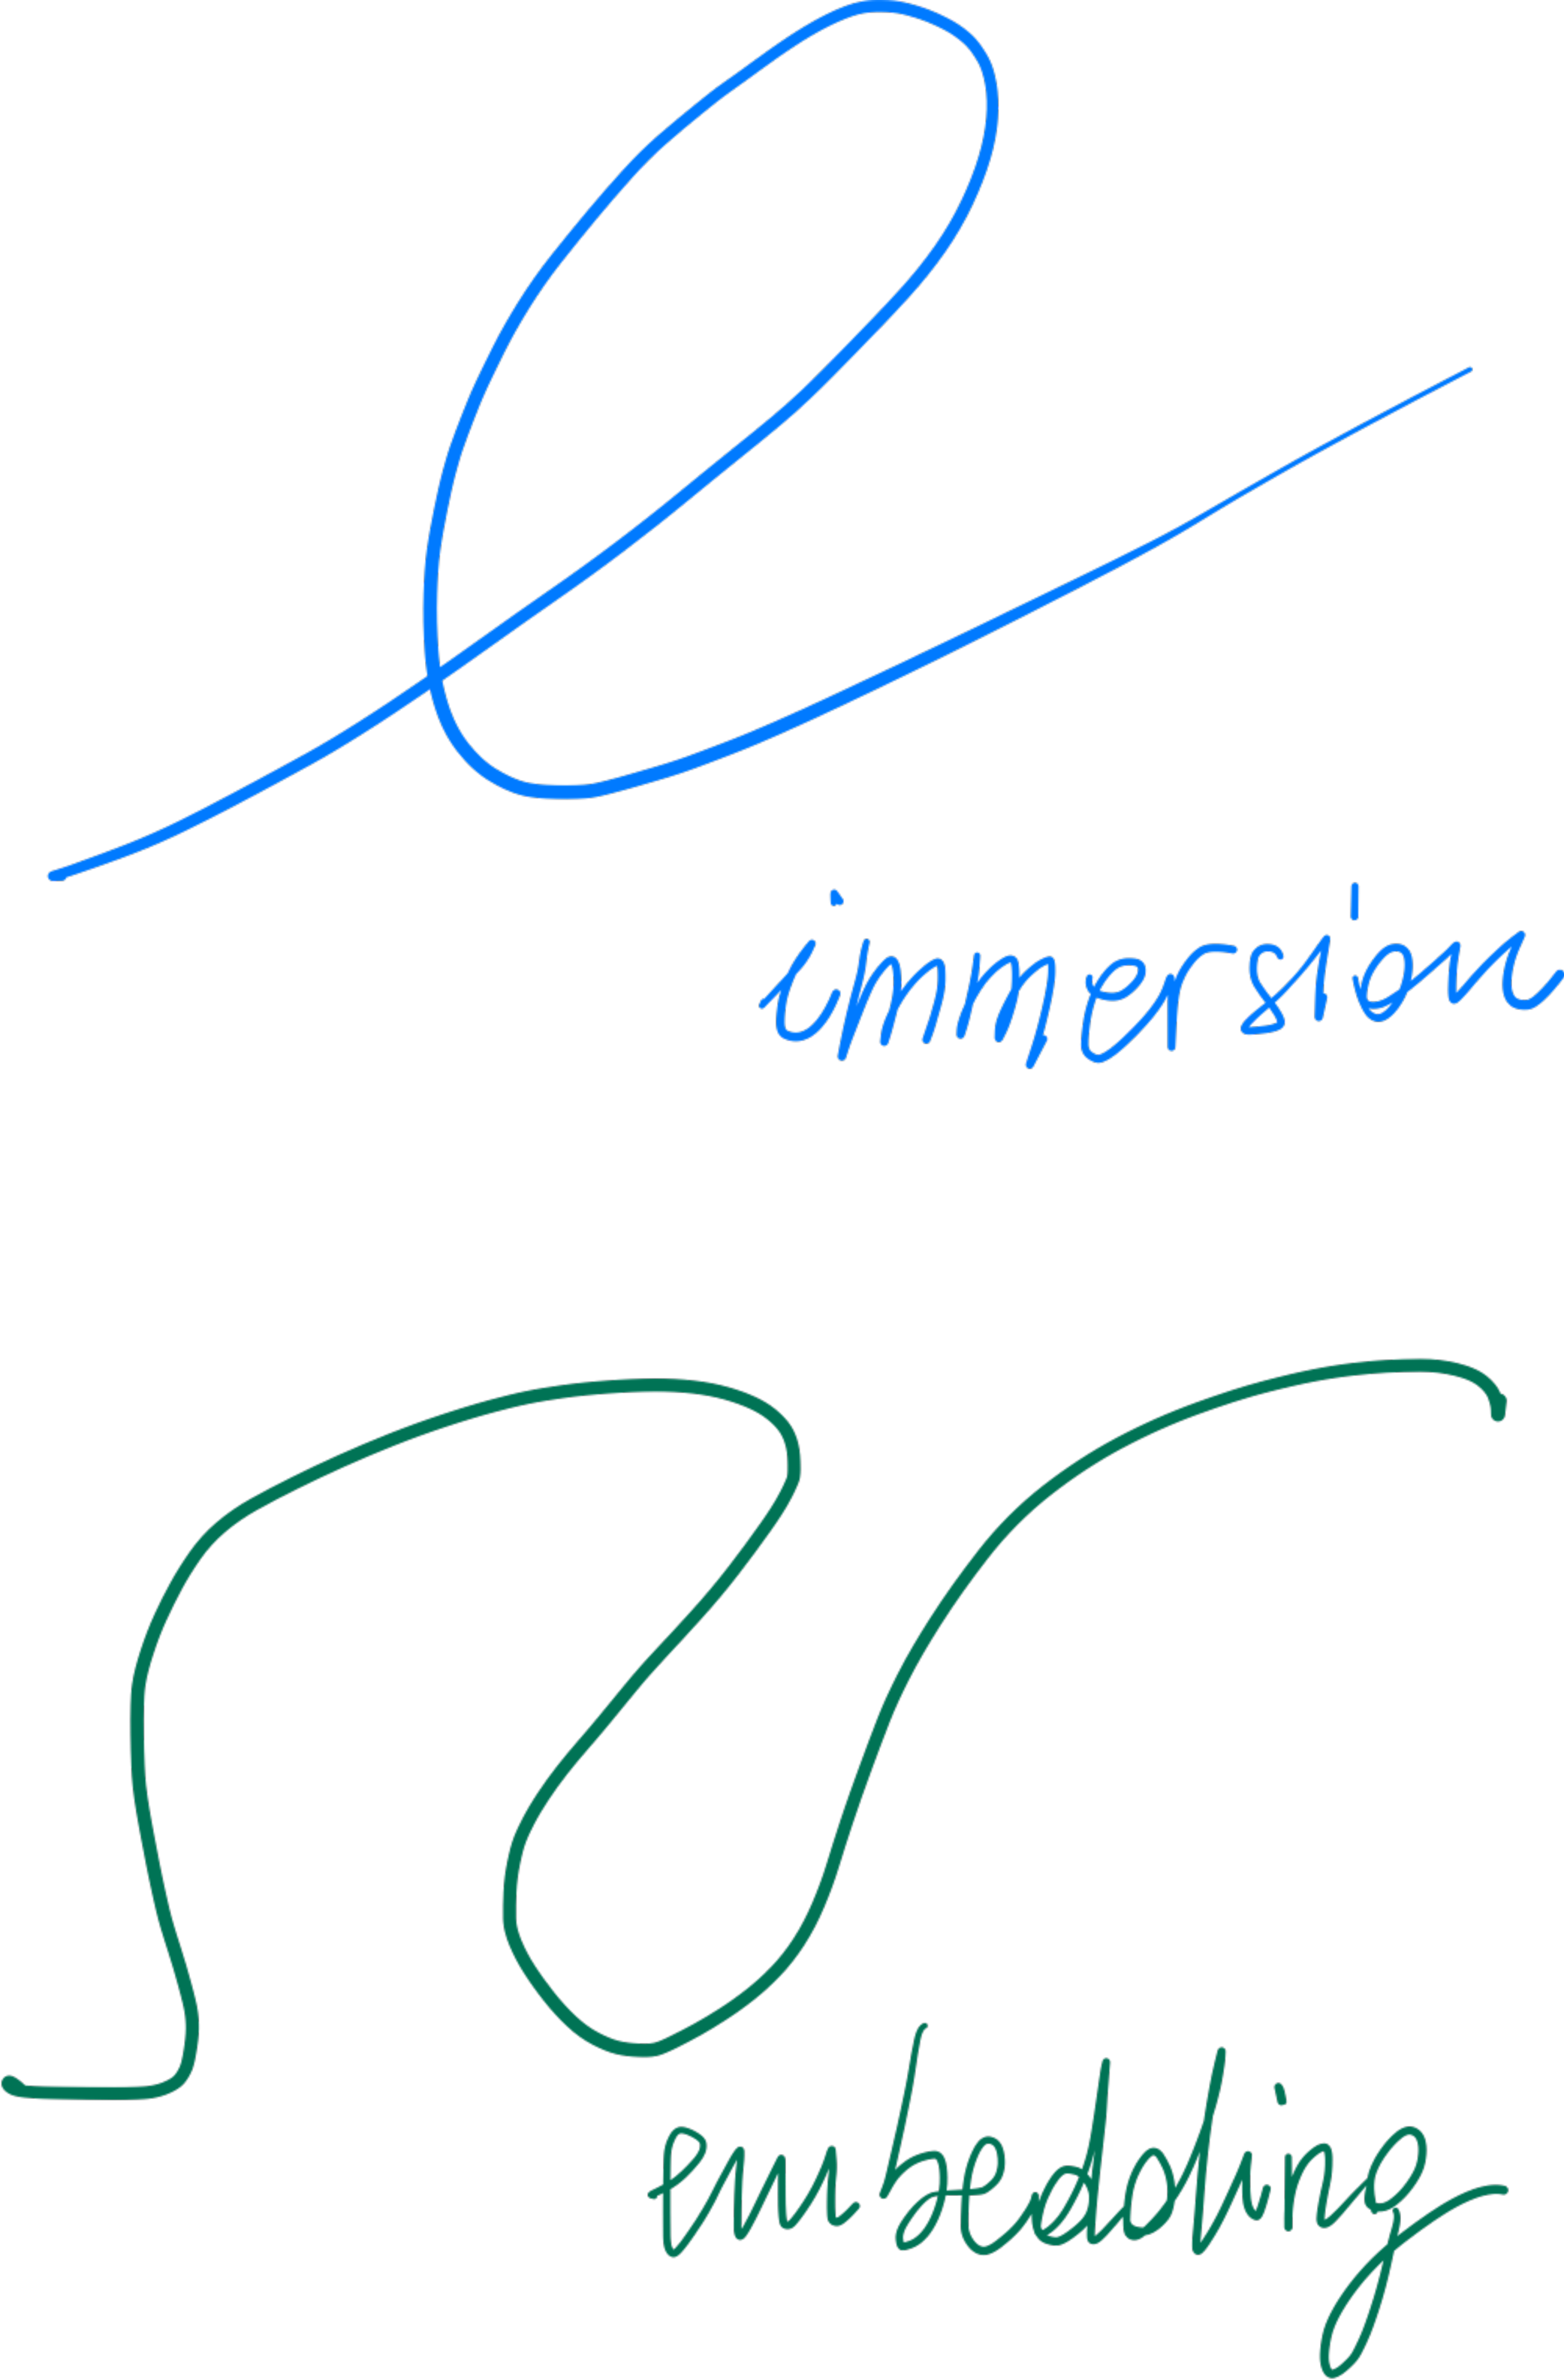
\includegraphics{2_8_1-immersion-embedding}
\end{marginfigure}

\begin{example}
  \begin{enumerate}
    \item The prototype of an immersion is the inclusion of $\R^m$ in a higher-dimensional $\R^n$:
    \begin{align}
      i &: \R^m \hookrightarrow \R^n,\\
      i &: \left(x^1, \ldots, x^m\right) \mapsto \left(x^1, \ldots, x^m, \LaTeXunderbrace{0, \ldots, 0}_{n-m}\right).
    \end{align}
    
    Indeed, the $n\times m$ matrix
    \begin{equation}
      di_x = Di(x)
       = \begin{pmatrix}
        1 & 0 & \cdots & 0 \\
        0 & 1 & \cdots & 0 \\
        \vdots & & \ddots & \vdots \\
        0 & \cdots & \cdots & 1 \\
        0 & \cdots & \cdots & 0 \\
        \vdots & & & \vdots \\
        0 & \cdots & \cdots & 0
       \end{pmatrix}
    \end{equation}
    has full rank (equal to $m$) and is therefore injective.
    Moreover, the map $i$ is injective and continuously invertible on its range, so it is also an embedding.

    \item The prototype for a submersion is the projection of $\R^m$ onto a lower-dimensional $\R^n$: $\pi\left(x^1,\ldots,x^n,x^{n+1},\ldots,x^m\right) = \left(x^1,\ldots,x^n\right)$.
    
    Indeed, the $n\times m$ matrix
    \begin{equation}
      d\pi_x = D\pi(x)
       = \begin{pmatrix}
        1 & 0 & \cdots & 0 & 0 & \cdots & 0 \\
        0 & 1 & \cdots & 0 & \vdots & & \vdots \\
        \vdots & & \ddots & \vdots & \vdots & & \vdots \\
        0 & \cdots & \cdots & 1 & 0 & \cdots & 0
       \end{pmatrix}
    \end{equation}
    has full rank (equal to $n$) and is therefore surjective.
    Hence, $i$ is a submersion.

    \item Let $n=1$, $m > 1$ and $\gamma:\R\to\R^m$ a smooth curve.
    The map $\gamma$ is an immersion if and only if its velocity vector satisfies $\gamma'(t)\neq0$ for all $t\in\R$.
    If the curve intersects itself, e.g $f(t_1) = f(t_2)$ for some $t_1\neq t_2$, then $f$ is not an embedding.
  \end{enumerate}
\end{example}

\begin{remark}
  Surjectivity of submersions or injectivity of immersions are properties of the differentials, not of the maps themselves.
  %
  For example, if $U\subset M$ open, the inclusion $i: U \to M$ is both an immersion and a submersion.
\end{remark}

\begin{definition}
  Let $M$ an $N$ smooth manifolds such that $M\subset N$ as a set.
  We say that $M$ is an \emph{embedded submanifold} of $N$ if the inclusion $M\hookrightarrow N$ is an embedding. If the inclusion is just an immersion, we say that $M$ is an \emph{immersed submanifold}.
\end{definition}

Before moving on, it is useful to recall some results from multivariable analysis.
A function $f:\R^m \to \R^n$ between euclidean spaces has rank $k$ at $x\in\R^m$ if its ($n\times m$) Jacobian matrix $Df(x)$ has rank $k$.
The function has \emph{maximal rank} at $x$ if $k = \min(n,m)$.
When $n=m$, $f$ has maximal rank at $x$ if and only if the square matrix $DF(x)$ is an invertible matrix.

As for many local properties, this definition carries over to manifolds rather ``smoothly''.

\begin{definition}
  A smooth map $F:M\to N$ has \emph{rank $k$} at a point $p$ if the linear subspace $dF_p(T_pM)$ has dimension $k$ inside $T_{F(p)}N$.
\end{definition}

And the same is true for the inverse function theorem:
compare the following statements.

\begin{theorem}[Inverse function theorem]\label{thm:ift}
  Let $U\subset\R^m$ open and $f:U \to \R^n$ be a smooth map.
  Assume that $f$ has maximal rank at some $x\in U$, then there exists a neighbourhood $\Omega\subset U$ of $x$ such that  $f\big|_\Omega : \Omega \to f(\Omega)$ is a diffeomorphism.
\end{theorem}

\begin{theorem}[Inverse function theorem for manifolds]\label{thm:iftm}
  Let $F:M\to N$ be a smooth function between manifolds of the same dimension $n$.
  Let $p\in M$ and assume that $F$ has maximal rank (i.e. rank $n$) at $p$.
  Then there exists a neighbourhood $V$ of $p$ such that the restriction $F:V\to F(V)$ is a diffeomorphism.
\end{theorem}
% \begin{proof}
%   This is a purely local statement.
%   Let $(U,\varphi)$ be a chart about $p\in M$ and let $(V, \psi)$ be a chart about $F(p)\in N$.
%   Since both $\varphi$ and $\psi$ are diffeomorphisms (and thus have maximal rank), the derivative of
%   \begin{equation}
%     \psi \circ F \circ \varphi^{-1}: \varphi(U\cap F^{-1}(V)) \to \psi(F(U)\cap V)
%   \end{equation}
%   has rank $n$ at $\varphi(p)$.
%   Thus the inverse function theorem, Theorem~\ref{thm:ift}, there exists $\Omega \subset \varphi(U\cap F^{-1}(V))$ such that $\psi \circ F \circ \varphi^{-1}\big|_{\Omega}$ is a diffeomorphism.
%   Therefore, once again since both $\varphi$ and $\psi$ are diffeomorphisms, $F\big|_W : W \to F(W)$ is also a diffeomorphism for $W := \varphi^{-1}(\Omega)$.
% \end{proof}
\begin{exercise}
  Use the euclidean inverse function theorem\footnote{Theorem~\ref{thm:ift}.} on $\R^n$ to prove Theorem~\ref{thm:iftm}.
\end{exercise}


In fact, also analogues of the implicit functions theorem carry over.
We will state them without going into the details of the proofs.

\begin{marginfigure}
  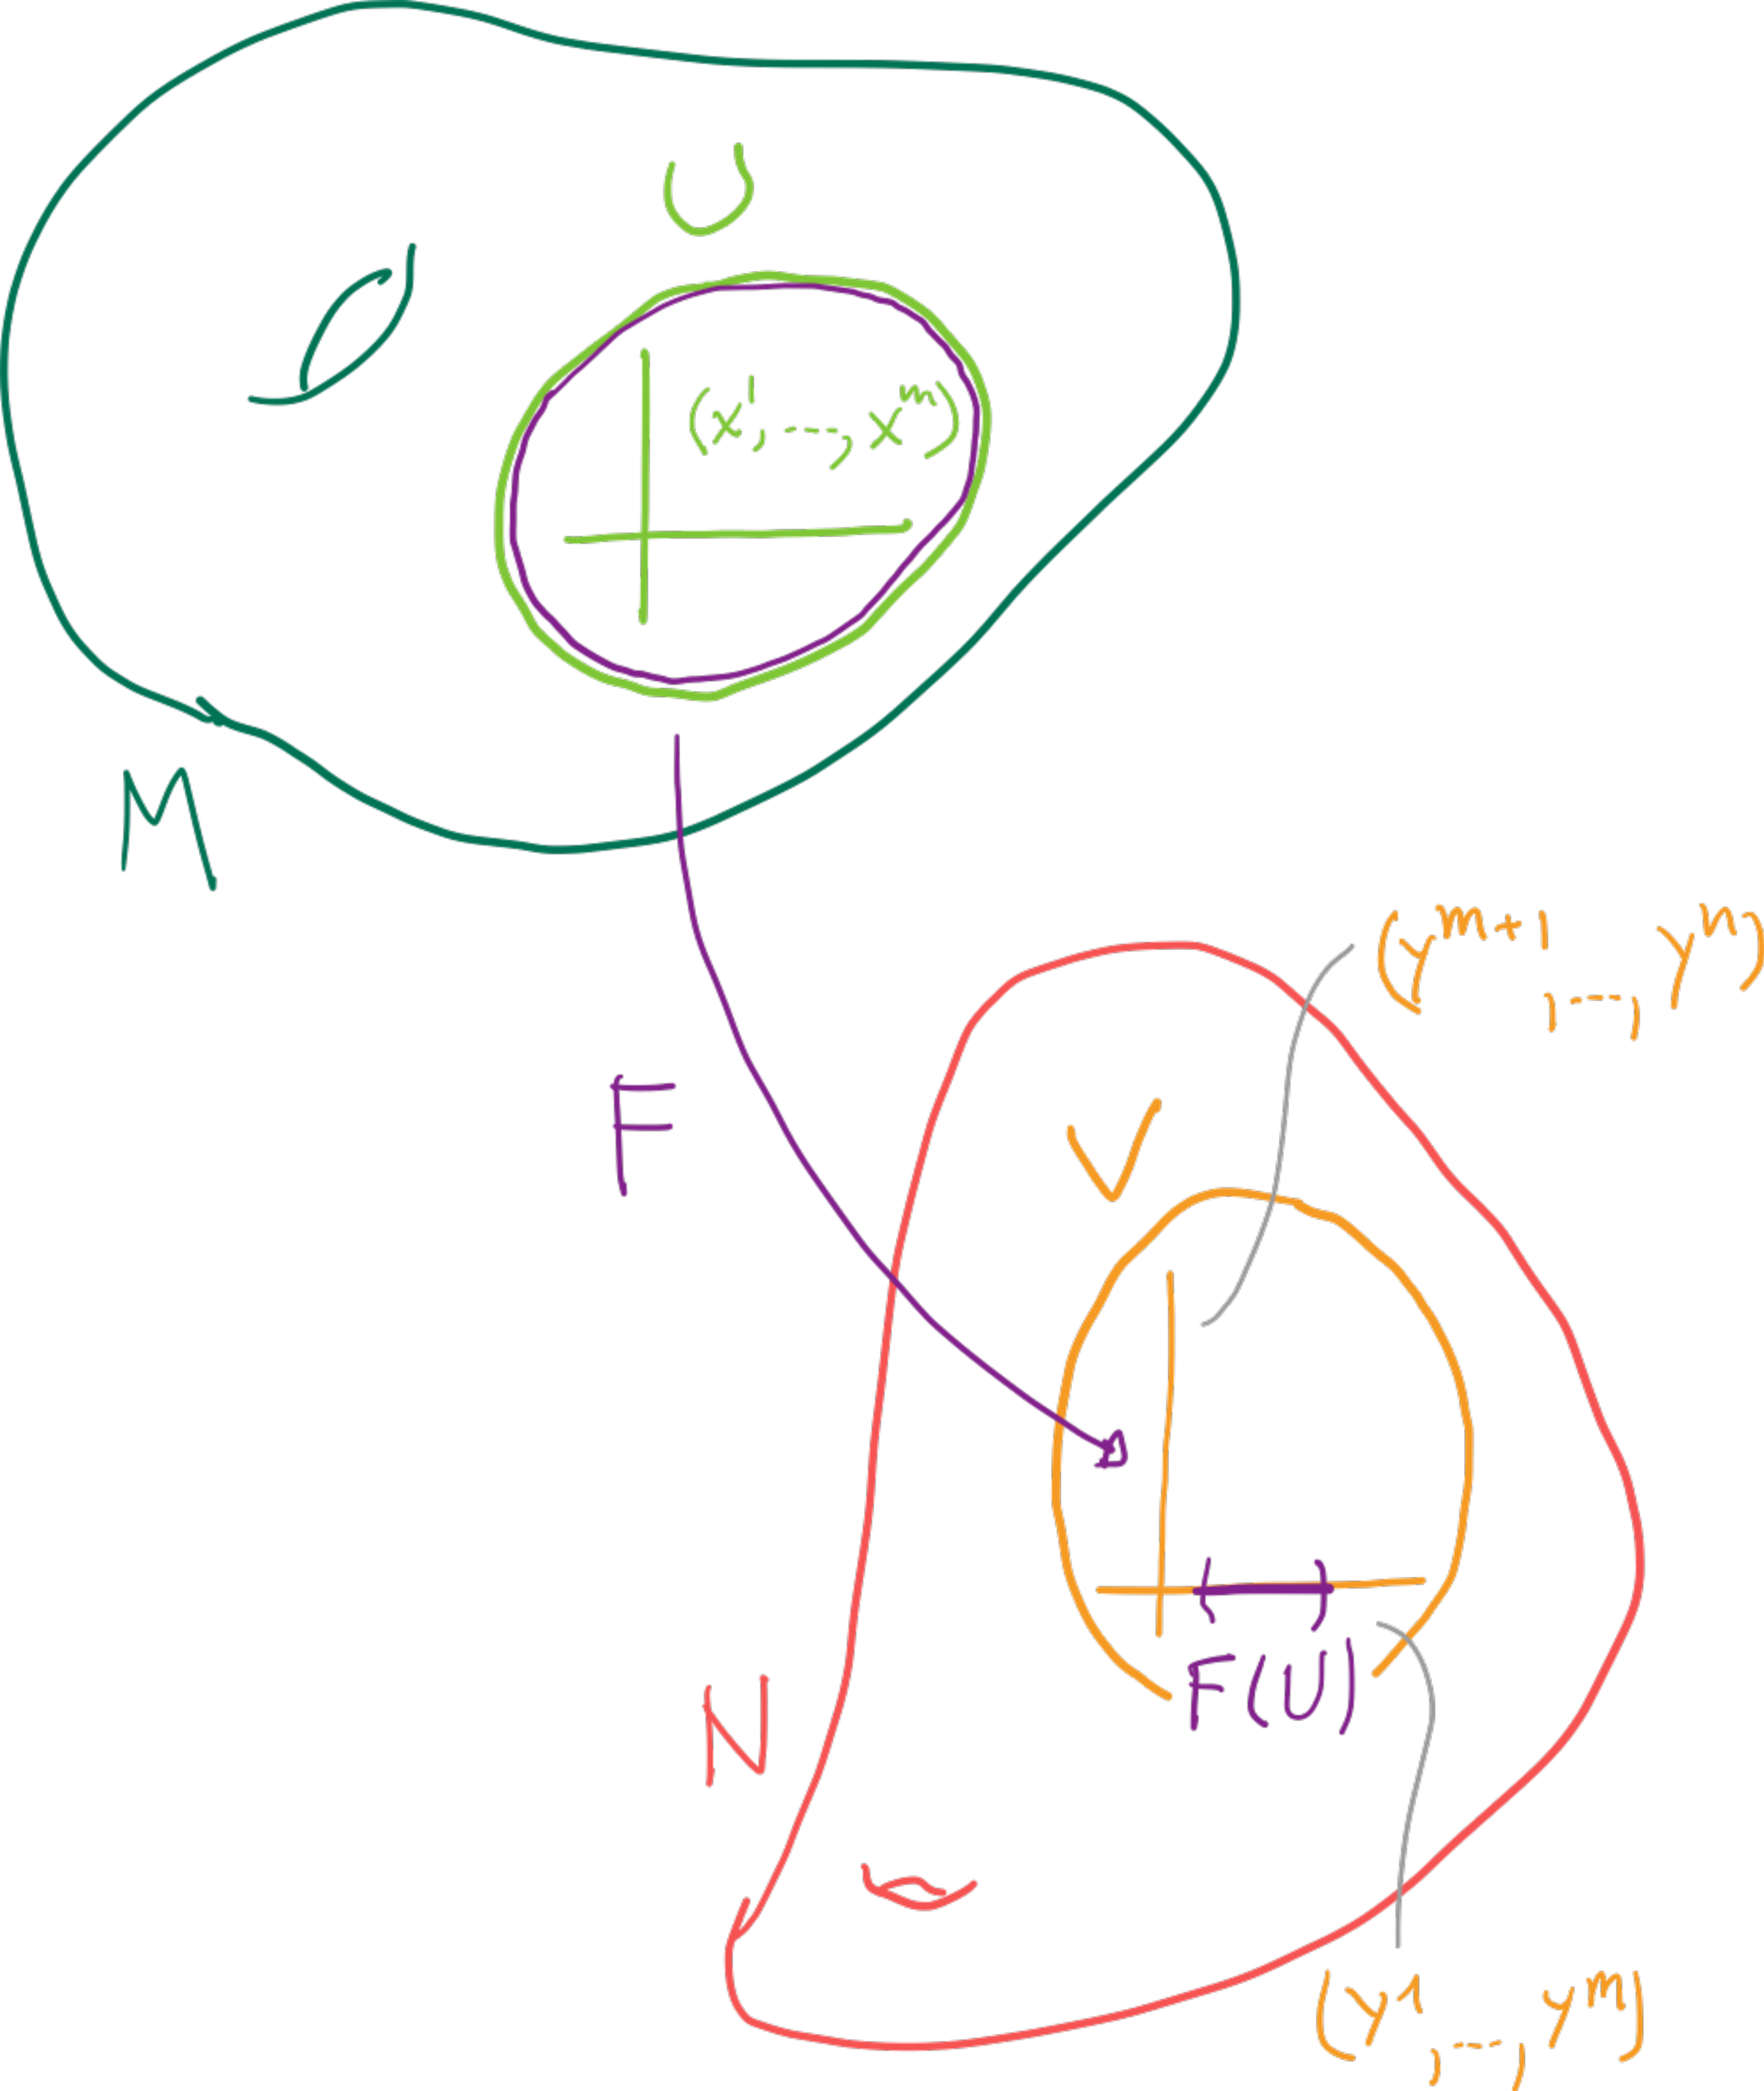
\includegraphics{2_8_9-mapping.pdf}
\end{marginfigure}
\begin{proposition}\label{prop:slice_chart}
  Let $F:M^m\to N^n$ be an immersion.
  Then for any $p\in M$, there exists a neighbourhood $U$ of $p$ and a chart $(V,\psi)$ about $F(p)\in N$ such that
  \begin{enumerate}[(i)]
    \item If $y^i = r^i\circ \psi$ are the local coordinates of $\psi$ then
    \begin{equation}\label{eq:slice_chart}
      F(U)\cap V = \left\{ q \in V \;\mid\; y^{m+1}(q)=\cdots=y^n(q)=0\right\};
    \end{equation}
    \item $F\big|_U$ is an embedding.
  \end{enumerate}
 \end{proposition}

If $F$ is an embedding, and this $M$ is an embedded submanifold, then the set $F(U)$ above can be written as $F(U) = F(M)\cap W$ for some open set $W\subset N$.
By replacing $V$ in~\eqref{eq:slice_chart} with $V\cap W$, one gets 
\begin{equation}
  F(M)\cap V = \left\{ q \in V \;\mid\; y^{m+1}(q)=\cdots=y^n(q)=0\right\}.
\end{equation}
In particular, this means that a $m$-dimensional submanifold is also a $m$-dimensional manifold whose charts are the ones above after we drop the final $n-m$ components.

The proposition above shows that an immersion is always a local embedding.
\begin{exercise}
  \begin{enumerate}
    \item If $M$ is compact, an injective immersion $F:M\to N$ is always an embedding.
    \item This is not necessarily the case in the non-compact case, give a counterexample.
  \end{enumerate}
\end{exercise}

\begin{lemma}
  With the notation of Proposition~\ref{prop:slice_chart}, assume that around any point $p\in M$ there is a chart of the form
  \begin{equation}
    M\cap V = \left\{ q \in V \;\mid\; y^{m+1}(q)=\cdots=y^n(q)=0\right\} \subset N.
  \end{equation}
  Then, if we endow $M$ with the subspace topology on $N$, $M$ is a topological manifold of dimension $m$.
  Furthermore, it has a smooth structure that makes it into an embedded submanifold of $N$.
\end{lemma}
\begin{proof}[Sketch]
  Let $\pi: \R^n\to\R^m$ be the projection as in the examples above.
  Let $p\in M$ and let $(V,\psi)$ be a chart with coordinates $(y^i)$ of the form above.
  If we endow $M$ with the subspace topology, then $\sigma:= \pi \circ \psi\big|_{M\cap V}$ is a homeomorphism.
  Repeating this at any point we end up with a collection of maps satisfying the hypotheses of Lemma~\ref{lem:manifold_chart}.
  Thus $M$ is a smooth manifold of dimension $n$ and its topology coincides with the subspace topology.

  Finally, with the inclusion $i:M\hookrightarrow N$ one has that $\psi \circ i\circ \sigma^{-1} (p^1,\ldots,p^n) = (p^1,\ldots,p^n,0,\ldots,0)$ which is smooth.
\end{proof}

A non-trivial consequence of the previous lemma is the following proposition\footnote{Refer to \cite[Proposition 5.8 and Proposition 5.31]{book:lee}.}.

\marginnote[1em]{In Proposition~\ref{prop:uniqdiffeoinclusion} it is not enough to ask that $\iota$ is smooth! As counterexample consider the two manifolds $(\R, \cA_1)$ with $\cA_1 := \{(\R, \id_\R)\}$ and $(\R, \cA_2)$ with $\cA_2 := \{(\R, x\mapsto x^3)\}$. The inclusion of open sets in $\R$ is smooth in both cases but is a diffeomorphism only in one.}
\begin{proposition}\label{prop:uniqdiffeoinclusion}
  Let $M$ be a manifold and $U\subset M$ an open set.
  Then $U$ has a unique differentiable structure such that the inclusion $\iota:U\hookrightarrow M$ is a diffeomorphism.
\end{proposition}

Up to this point, the first manifold had the same dimension or was smaller than the second one.
What if it is larger?

\begin{definition}
  Let $F:M^m \to N^n$ be a smooth map between smooth manifolds.
  A point $p\in M$ is said to be a \emph{regular point} of $F$ if $F$ has rank $n$ at $p$ (which implies that $m\geq n$), while it is called a \emph{critical point} if it is not.

  Similarly, a point $q\in N$ is called a \emph{regular value} if every point in $F^{-1}(q)$ is a regular point, and \emph{critical value} otherwise. If $q\not\in F(M)$, then $q$ is considered a regular value (in the sense that there is nothing to check in its preimage by $F$).
  Cf. Figure~\ref{fig:2_8-crit_pts}.
\end{definition}
\begin{marginfigure}[12em]
  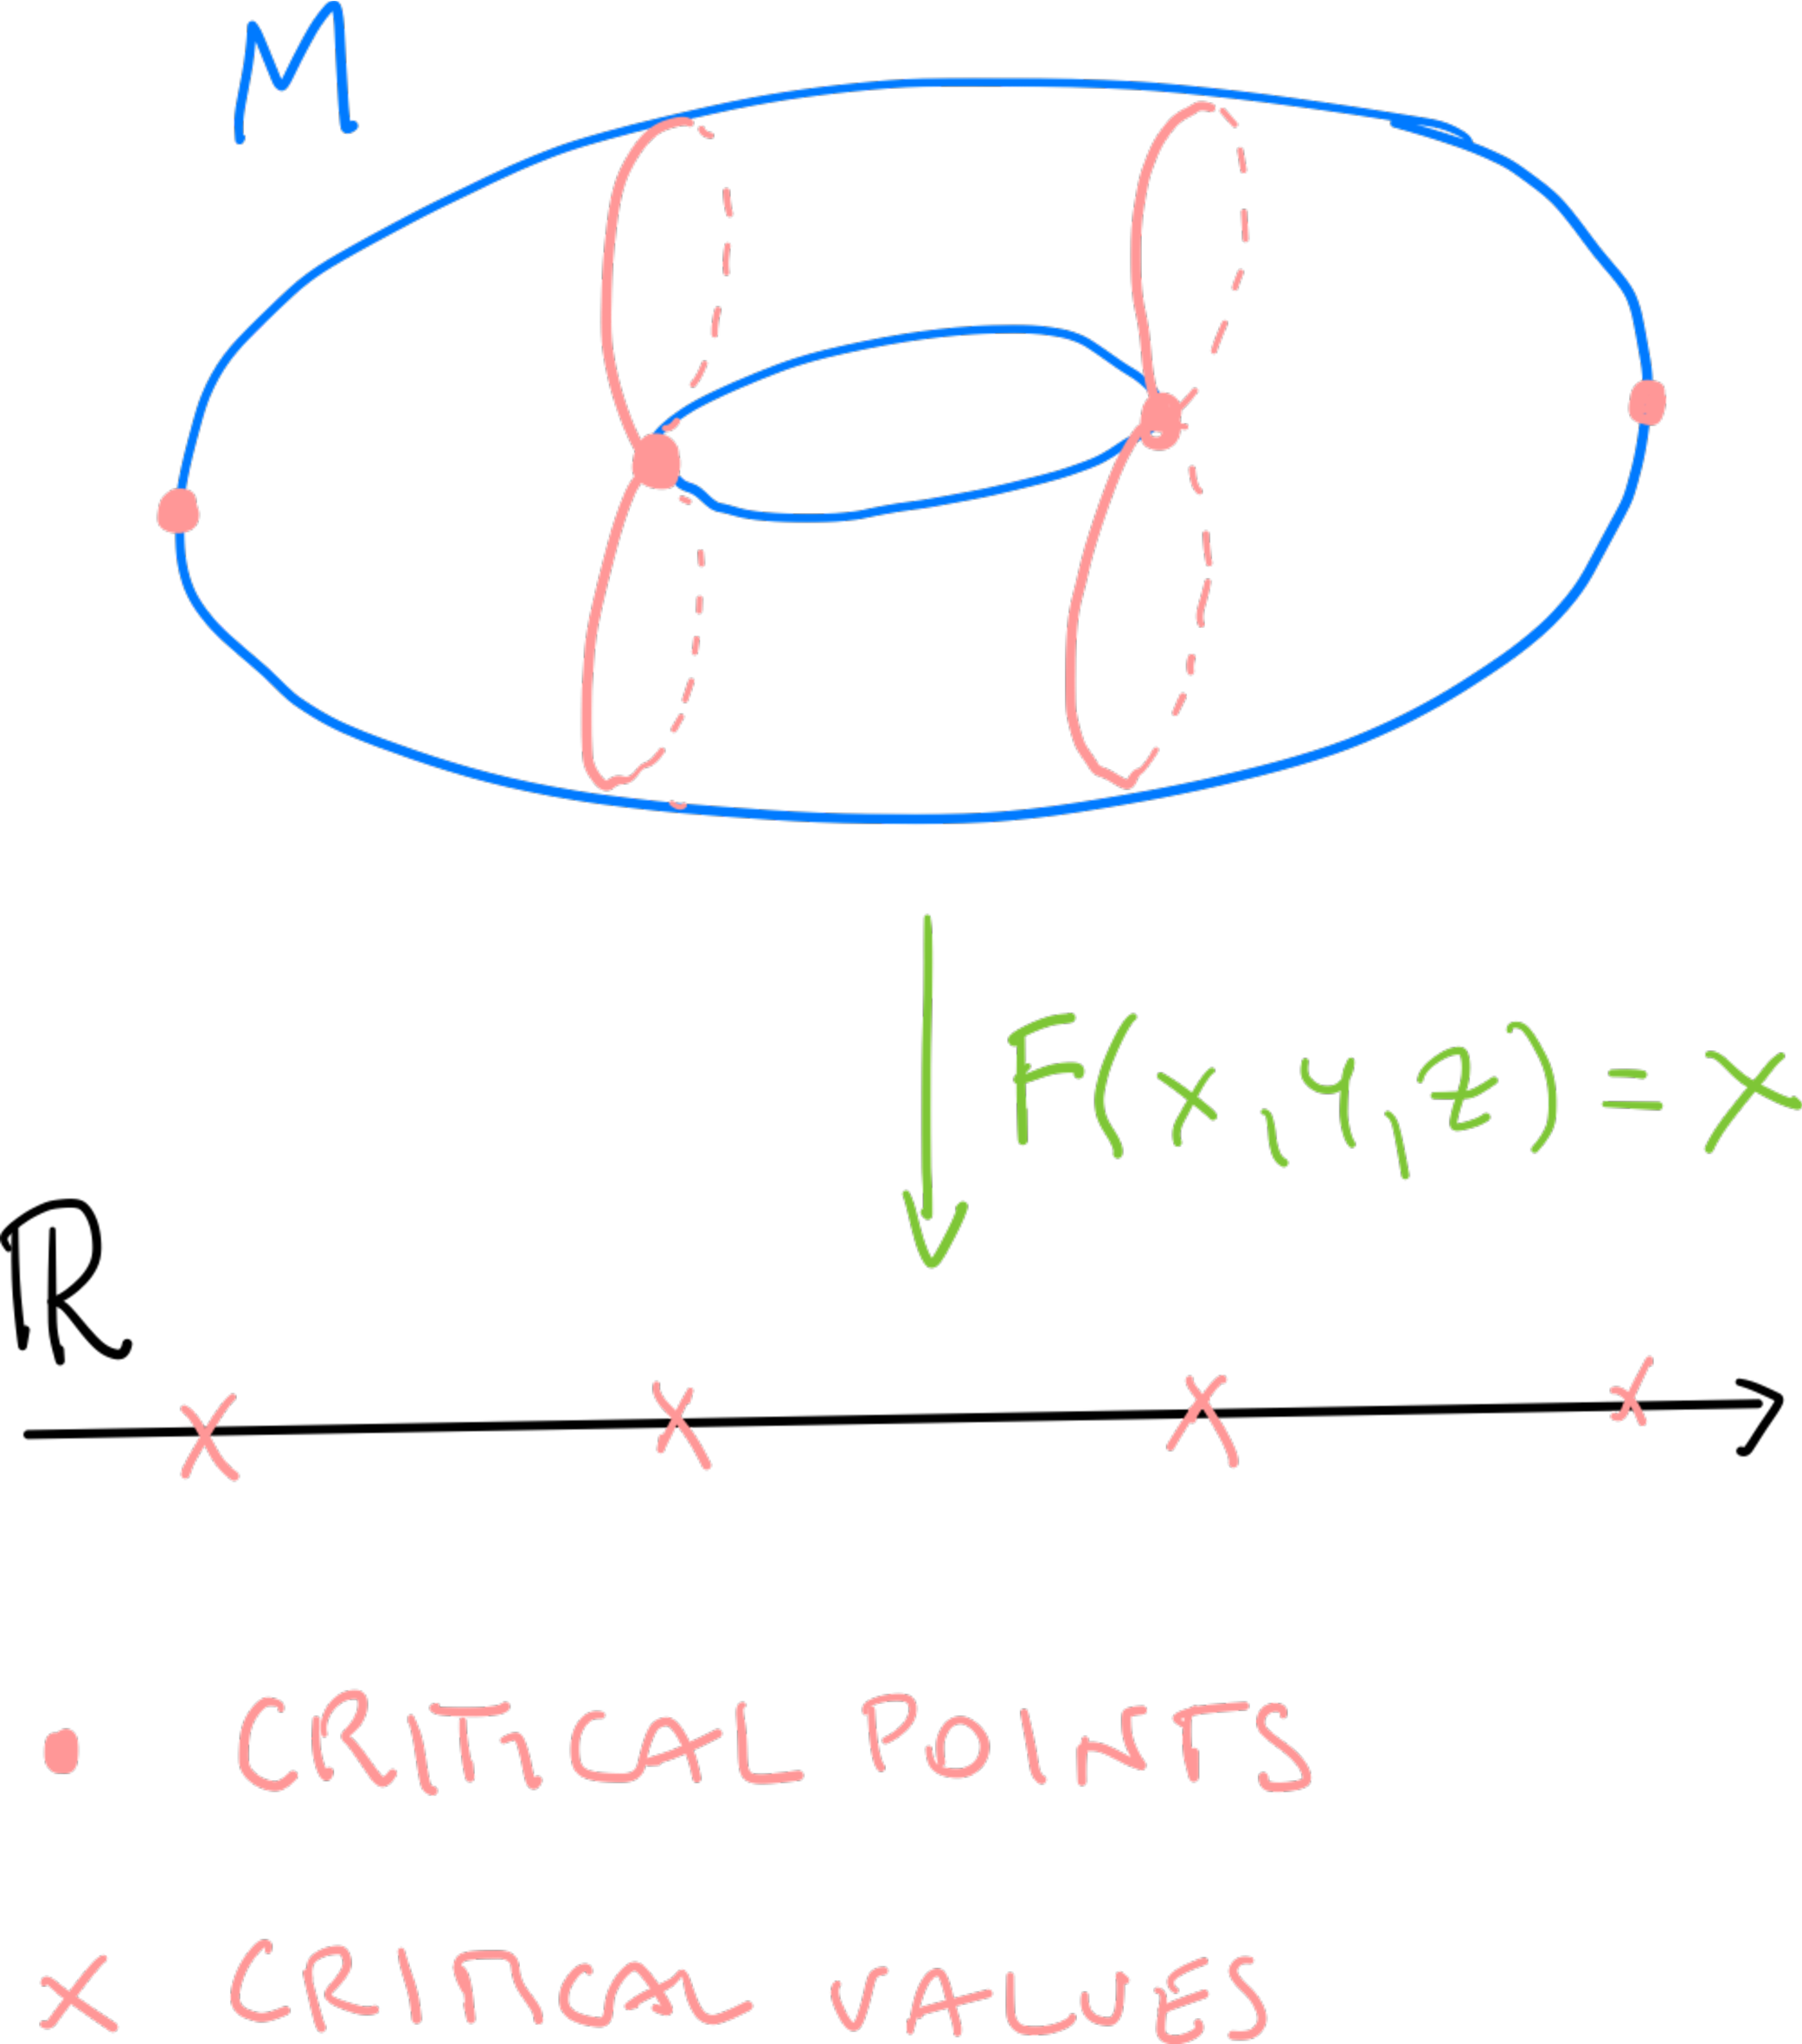
\includegraphics{2_8-crit_pts.pdf}
  \caption{Beware of the subtleties here. The map $F=\pi_x\circ i$ for the inclusion $i:\bT^2\hookrightarrow\R^3$ and the projection $\pi_x(x,y,z)=x$.
  So $dF_p = d (\pi_x)_{i(p)} \circ d i_p$. The latter is zero if $d i_p: T_p\bT^2\hookrightarrow T_p\R^3$ is, which happens when the image of $T_p\bT^2$ is contained in the $yz$-plane (the reason will be clear by the end of the chapter): the critical points depicted here are exactly those points for which the tangent plane is the $yz$-plane.}
  \label{fig:2_8-crit_pts}
\end{marginfigure}

With this definition at hand, we are ready to state one of the most important theorems in this lecture. Differently from most previous ones, the statement is not local.

\begin{theorem}[Implicit function theorem for manifolds]\label{thm:impl_fun}
  Let $m\geq n$ and let $F: M^m \to N^n$ be a smooth map between smooth manifolds.
  If $q\in N$ is a regular value of $F$ and $P := F^{-1}(q)$ is not empty, then $P$ is a topological manifold of dimension $n-k$. 
  Moreover, there exists a smooth structure on $P$ which makes it into a smooth embedded submanifold of $M$.
\end{theorem}

\begin{remark}
  If $F:M\to N$ is a submersion, Theorem~\ref{thm:impl_fun} implies that any $p\in M$ belongs to the $(n-k)$-dimensional embedded submanifold $F^{-1}(F(p))$.
\end{remark}

From this observation follows another interesting proposition, again consequence of the inverse and the implicit function theorems, of which we will also omit the proof.

\begin{proposition}\label{prop:submanifolds_and_R}
  The following assertions are equivalent.
  \begin{enumerate}[(i)]
    \item $M^k\subset N^n$ is a $k$-dimensional submanifold.
    \item $M$ is locally the image of an embedding of a subset of $\R^k$.
    That is, for every $p\in M$ there exists $V\subset M$ open neighbourhood of $p$, an open set $U\subset\R^k$ and an embedding
    \begin{equation}
      \varphi : U \to N \quad\mbox{such that}\quad \varphi(U)=V.
    \end{equation}
    \item $M$ is locally a level set of a submersion into $\R^{n-k}$.
    That is, for every $p\in M$ there exists $V\subset M$ open neighbourhood of $p$ and a submersion $\varphi: V \to\R^{n-k}$ such that
    \begin{equation}
      M\cap V = \{q\in V \;\mid\; \varphi(q) = 0\}.
    \end{equation}
  \end{enumerate}
\end{proposition}

\begin{remark}\label{rmk:WhitneyET}
  Whitney Embedding Theorem states that any smooth $n$-dimensional manifold can be smoothly embedded into $\R^{2n}$.
  Thus any abstract manifold is diffeomorphic to a submanifold of $\R^m$ (for some $m$).
\end{remark}

\begin{example}\label{ex:s2}
  The sphere $\bS^2 = \{x\in\R^3 \mid \|x\| = 1\}$ is a $2$-dimensional submanifold of $\R^3$.
  This is immediate using the third condition in the Proposition~\ref{prop:submanifolds_and_R}: let $\varphi(x) = \|x\|^2 -1 : \R^3 \to \R$, then $\varphi$ is smooth, $\bS^2 = \{F(x)=0\}$ and $dF_x(v)= 2x\cdot v \neq 0$ for $x\in\bS^2$.
\end{example}

\begin{example}
  Let $N = \R^2$ and $M = \{ x\in M \;\mid\; x^2 = |x^1| \}$.
  Then $M$ is \emph{not} a submanifold, but it can be equipped with a manifold structure.
  For example with the global atlas $\{(M,\; (x^1,x^2)\mapsto x^1)\}$, $M$ is a manifold diffeomorphic to $\R$.
\end{example}

\begin{exercise}
  A real-valued function $f:M\to\R$ on a manifold has a local maximum at $p\in M$ if there is a neighbourhood $U\subset M$ of $p$ such that $f(p) \geq f(q)$ for all $q\in U$.
  \begin{enumerate}
    \item Show that if a differentiable function $f:(a,b)\to\R$, has a local maximum at $x\in (a,b)$, then $f'(x) = 0$.
    \item Prove that a local maximum of a function $f\in C^\infty(M)$ is a critical point of $f$.\\
    \textit{\small Hint: choose $X_p\in T_pM$ and let $\gamma(t)$ be a curve in $M$ starting at $p$ with initial velocity $X_p$. The $f\circ \gamma$ is a real-valued function with local maximum at $0$...}
  \end{enumerate}
\end{exercise}

Of course, we can also define subbundles.
\begin{definition}
  Let $\pi:E \to M$ be a rank-$n$ vector bundle and $F\subset E$ a submanifold.
  If for all $p\in M$, the intersection $F_p := F\cap E_p$ is a $k$-dimensional subspace of the vector space $E_p$ and $\pi|_F : F \to M$ defines a rank-$k$ vector bundle, then $\pi|F: F \to M$ is called a \emph{subbundle} of $E$.
\end{definition}

\begin{exercise}[\textit{[homework 2]}]
  Let $M$ be a smooth $m$-manifold and $N$ a smooth $n$-manifold.
  Let $F:M\to N$ be an embedding and denote $\widetilde M = F(M)\subset N$.
  \begin{enumerate}[(a)]
    \item Show that the tangent bundle of $M$ in $N$, given by $T\widetilde M := dF(TM) \subset TN\Big|_{\widetilde M}$, is a subbundle of $TN\Big|_{\widetilde M}$ by providing explicit local trivialisations in terms of the charts $(U, \varphi)$ for $M$.
    \item Assume that there exist a smooth function $\Phi:N\to\R^{n-k}$ such that $\widetilde M := \{p\in N \mid \Phi(p) = 0\}$ and $d\Phi_p$ has full rank for all $p\in\widetilde M$. Prove that
    \begin{equation}
      T\widetilde{M} = \{(p,v)\in TN|_{\widetilde{M}} \mid v\in\ker(d\Phi_p)\}.
    \end{equation}
  \end{enumerate}
\end{exercise}

We still have a question pending since the beginning of the chapter.
Is the tangent space to a sphere the one that we naively imagine (see Figure~\ref{fig:tan-embedded-sphere})?
To finally answer the question, we will prove one last proposition.

\begin{proposition}
  Let $F:M^m\to N^n$ be a smooth map between manifolds.
  Let $q\in N$ be a regular value of $F$ such that $P:=F^{-1}(q)\neq\emptyset$ and let $i:P\hookrightarrow M$ denote the inclusion.
  Then, for all $p\in P$, one has
  \begin{equation}
    d i_p(T_p P) = \ker dF_p.
  \end{equation}
\end{proposition}
\begin{proof}
  Both $d i_p(T_p P)\subset T_p M$ and $\ker dF_p \subset T_p M$ are linear subspaces of the same dimension $n-k$, therefore we only need to show that one contains the other, e.g. $d i_p(T_p P) \subset \ker dF_p$.

  Take $f\in C^\infty(N)$ and $v\in T_p P$. By the chain rule\footnote{Proposition~\ref{thm:chainrule_mfld}} we get
  \begin{equation}
    (d F_p \circ d i_p)(v)(f) = d(F\circ i)_p(v)(f) = v(f\circ F\circ i).
  \end{equation}
  Since $F\circ i\big|_{P} \equiv q$ constant, $f\circ F\circ i\in C^\infty(P)$ is the constant function $p \mapsto f(q)$ and by Corollary~\ref{cor:derzero} we have $v(f\circ F\circ i)=0$.
\end{proof}

\begin{example}
  We have seen in Example~\ref{ex:s2} that $\bS^2 = F^{-1}(0)$ is a smooth manifold of dimension $2$.
  Denoting the inclusion by $i:\bS^2 \hookrightarrow\R^3$, one has
  \begin{equation}\label{ex:tan_sph}
    di_x(T_x\bS^2) = \cT_p(p^\perp)
  \end{equation}
  where $\cT_p:\R^3\to T_p\R^3$ is the map defined in Exercise~\ref{ex:tg_curve_iso} and
  \begin{equation}
    p^\perp := \big\{q\in\R^3 \;\mid\; \left\langle p, q\right\rangle = 0\big\},
  \end{equation}
  where $\left\langle\cdot,\cdot\right\rangle$ is the usual Euclidean dot product.
  Take a long deep breath and unfold the definitions in~\eqref{ex:tan_sph}, here it may be useful to draw a picture\footnote{Which is generally always the case in geometry and topology, and most other mathematical fields.}. 
  Equation~\eqref{ex:tan_sph} implies that the tangent space to $\bS^2$ at a point $x$  is the plane tangent to $\bS^2$ at $p$, as claimed in Figure~\ref{fig:tan-embedded-sphere}.
\end{example}

\begin{exercise}
  Show that the above reasoning holds verbatim for $\bS^n\subset\R^{n+1}$.
\end{exercise}

\begin{exercise}
  Let $U\subset\R^n$ open and $f:U\to\R$ smooth.
  Define $g:U\to\R^{n+1}$ by
  \begin{equation}
    g(x) = (x, f(x)).
  \end{equation} 
  Show that $g$ is a smooth embedding and, therefore, that $g(U)$ is a smooth embedded $n$-dimensional submanifold\footnote{$g(U)$ is the the \emph{graph} of $f$!} of $\R^{n+1}$.
\end{exercise}

\begin{exercise}[\textit{[homework 2]}]\label{exe:onsubmanifold}
  Show that the orthogonal matrices $O(n) := \{ Q\in GL(n) \mid Q^TQ=\id \}$ form a $n(n-1)/2$-dimensional submanifold of the $n^2$-manifold $\mathrm{Mat}(n)$ of $n\times n$-matrices.

  Show also that
  \begin{equation}
    T_Q O(n) = \left\lbrace B \in \mathrm{Mat}(n) \mid (Q^{-1} B)^T = -Q^{-1}B \right\rbrace,
  \end{equation}
  and, thus, that $T_{\id} O(n)$ is the space of skew-symmetric matrices
  \begin{equation}
    T_{\id} O(n) = \left\{ B \in \mathrm{Mat}(n) \mid B^T = -B \right\}.
  \end{equation}
  \textit{\small Hint: Find a suitable map $F: \mathrm{Mat}(n) \to \mathrm{Sym}(n)$ such that $F^{-1}(\{p\}) = O(n)$ for some point $p$ in the image, e.g. $0$ or $\id_n$.
  Here $\mathrm{Sym}(n)$ denotes the space of symmetric matrices.}
\end{exercise}


\chapter{Cotangent bundle}

\chapter{Vector fields}

\chapter{Tensor products}

\chapter{Differential Forms}

\subsection{de Rahm cohomology}

\chapter{Integration of forms}
\subsection{Orientation}

\subsection{Stokes' Theorem}

\begin{appendices}
  \chapter{Solution to selected exercises}
  \section{Chapter \ref{ch:manifolds}}
  
  \newthought{Exercise \ref{exe:rntopsp}.}
  \begin{enumerate}
    \item[] Hausdorff. For $x\neq y\in\R^n$, let $\epsilon = d(x,y)/3$.
    Then the two balls $B_x(\epsilon) := \{z\in X \;\mid\; d(z,x)<\epsilon\}$ and $B_y(\epsilon)$ are disjoint open sets containing $x$ and $y$ respectively.
    \item[] Second countable. As countable basis for the topology we can take the open balls $B_\epsilon(x)$ with rational radii $\epsilon\in\Q$ and centers $x\in\Q^n$.
  \end{enumerate}
  
\end{appendices}

\bibliographystyle{plainnat}
\bibliography{aom}
\addcontentsline{toc}{chapter}{Bibliography}
\end{document}